\documentclass[letterpaper, 12pt, oneside]{book}
\usepackage[top=1in, left=0.9in, right=1.25in, bottom=1in]{geometry}
\usepackage{bachelorstitlepageUNAM}
\usepackage{titlesec} % Quita palabra «Capítulo» de \chapter
\titleformat{\chapter} % Config titlesec
	{\Large\bfseries}	%
	{\huge \thechapter}	%
	{20pt}				%
	{\huge}				%
\usepackage[utf8x]{inputenc}
\author{Sergio Miguel Fernández Martínez}
\title{
Métodos de aprendizaje por refuerzo profundo para el control del sistema dinámico de vuelo de un cuadricóptero}
\faculty{Facultad de Ciencias}
\degree{Licenciado en Matemáticas Aplicadas}
\supervisor{Dr. Antonio Capella Kort}
\cityandyear{Ciudad Universitaria, Ciudad de México, 2026}
\logouni{Escudo-UNAM}
\logofac{Escudo-FCIENCIAS}


\usepackage[english, spanish, es-nodecimaldot]{babel}
\AtBeginDocument{\shorthandoff{>}}
\usepackage{pdfpages} % <-- for the front paige
\usepackage{listings}
\usepackage{newtxtt}
\usepackage{multicol}
\usepackage{amsmath}
\usepackage{amssymb}
\usepackage{amsfonts}
\usepackage{hyperref}
\usepackage[spanish]{cleveref}
\usepackage{dsfont}
\usepackage{tocloft}
\usepackage{subcaption}
\usepackage{multicol}
\usepackage{multirow}
\usepackage{aurical}
\usepackage{setspace}

\usepackage[acronym]{glossaries}

\crefformat{equation}{ecuación~#2#1#3}
\Crefformat{equation}{Ecuación~#2#1#3}
\crefrangeformat{equation}{ecuaciones #3#1#4 a #5#2#6}
\newcommand{\eqreftext}[1]{ecuación~\ref{#1}}

\usepackage{cite}
\graphicspath{ {figures/} }
\usepackage{array}

\setlength{\parskip}{1em}

\usepackage{xcolor}
\definecolor{light-gray}{gray}{0.95}
\newcommand{\code}[1]{\colorbox{light-gray}{\texttt{#1}}}


\definecolor{codegreen}{rgb}{0,0.6,0}
\definecolor{codegray}{rgb}{0.5,0.5,0.5}
\definecolor{codepurple}{rgb}{0.4,0.4,0.4}
\definecolor{backcolour}{rgb}{0.98,0.98,0.98}

\lstdefinestyle{mystyle}{
    backgroundcolor=\color{backcolour},
    commentstyle=\color{codegray},
    numberstyle=\tiny\color{codegray},
    stringstyle=\color{codepurple},
    basicstyle=\fontsize{9}{11}\selectfont,
    keywordstyle=\bfseries,
    breakatwhitespace=false,
    breaklines=true,
    captionpos=b,
    keepspaces=true,
    numbers=left,
    numbersep=5pt,
    showspaces=false,
    showstringspaces=false,
    showtabs=false,
    tabsize=2
}

\lstset{style=mystyle}

\usepackage{bm}
\newcommand\tab[1][1cm]{\hspace*{#1}}
\usepackage{float, graphicx, multicol}
\usepackage{amsthm,enumerate}


\usepackage[spanish,onelanguage, linesnumbered,ruled,vlined]{algorithm2e}
\newcommand\mycommfont[1]{\footnotesize\ttfamily\textcolor{gray}{#1}}
\SetCommentSty{mycommfont}

\DeclareMathOperator*{\argmax}{arg\,max}
\DeclareMathOperator*{\argmin}{arg\,min}


\setlength{\columnsep}{30pt}

%% Multi layer perceptron
\usepackage{latexsym}

\usepackage{tikz}
\usepackage{tikz-3dplot}
\usetikzlibrary{decorations.pathreplacing}
\usetikzlibrary{fadings}
\usetikzlibrary{3d,perspective,calc}
%%

\newcommand*{\horzbar}{\rule[.5ex]{2.5ex}{0.5pt}}



%\title{Aproximación de políticas para sistemas de control con aprendizaje por refuerzo *}
%\author{Sergio Miguel Fernández Martínez \\ Amilkar Gazque }
%\date{Febrero 2021}


\usepackage[nottoc]{tocbibind}

%\geometry{
% letterpaper,
% left=25mm,
% right=25mm,
% top=25mm,
% }

\renewcommand\qedsymbol{$\blacksquare$}

\theoremstyle{plain}
\newtheorem{theorem}{Teorema}[section]
\newtheorem{prop}{Proposición}[section]
\newtheorem{definition}{Definición}[section]
\newtheorem{remark}{Observación}[section]
\newtheorem{corollary}{Corolario}[section]
\newtheorem{example}{Ejemplo}[section]
\newtheorem{lemma}[theorem]{Lemma}
\renewcommand\qedsymbol{$\blacksquare$}


\def\upint{\mathchoice%
    {\mkern13mu\overline{\vphantom{\intop}\mkern7mu}\mkern-20mu}%
    {\mkern7mu\overline{\vphantom{\intop}\mkern7mu}\mkern-14mu}%
    {\mkern7mu\overline{\vphantom{\intop}\mkern7mu}\mkern-14mu}%
    {\mkern7mu\overline{\vphantom{\intop}\mkern7mu}\mkern-14mu}%
  \int}
\def\lowint{\mkern3mu\underline{\vphantom{\intop}\mkern7mu}\mkern-10mu\int}

\newcommand{\bigzero}{\mbox{\normalfont\Large\bfseries 0}}
\newcommand{\rvline}{\hspace*{-\arraycolsep}\vline\hspace*{-\arraycolsep}}



\makenoidxglossaries
\newglossaryentry{sym-state}{
  name={\ensuremath{x_t}},
  description={Vector de estado del sistema en el instante \ensuremath{t}, con \ensuremath{x_t\in\mathbb{R}^{n_x}}}
}
\newglossaryentry{sym-action}{
  name={\ensuremath{u_t}},
  description={Vector de control aplicado en el instante \ensuremath{t}, con \ensuremath{u_t\in\mathbb{R}^{n_u}}}
}
\newglossaryentry{sym-policy}{
  name={\ensuremath{\pi_\theta}},
  description={Política parametrizada por \ensuremath{\theta}}
}
\newglossaryentry{sym-reward}{
  name={\ensuremath{r_t}},
  description={Recompensa instantánea en el tiempo \ensuremath{t}}
}
\newglossaryentry{sym-value}{
  name={\ensuremath{V^\pi(\mathbf{x})}},
  description={Función de valor de estado bajo la política \ensuremath{\pi}}
}
\newglossaryentry{sym-qvalue}{
  name={\ensuremath{Q^\pi(\mathbf{x},\mathbf{u})}},
  description={Función de valor acción-estado bajo la política \ensuremath{\pi}}
}
\newacronym{adam}{ADAM}{\textit{Adaptive Moment Estimation}}
\newacronym{admm}{ADMM}{\textit{Alternating Directions Method of Multipliers}}
\newacronym{ann}{ANN}{\textit{Artificial Neural Network}}
\newacronym{badmm}{BADMM}{\textit{Bregman Alternating Directions Method of Multipliers}}
\newacronym{dl}{DL}{\textit{Deep Learning}}
\newacronym{ddpg}{DDPG}{\textit{Deep Deterministic Policy Gradient}}
\newacronym{dqn}{DQN}{\textit{Deep Q-Networks}}
\newacronym{dpg}{DPG}{\textit{Deterministic Policy Gradient}}
\newacronym{ilqr}{iLQR}{\textit{Iterative Linear Quadratic Regulator}}
\newacronym{glie}{GLIE}{\textit{Greedy in the Limit with Infinite Exploration}}
\newacronym{gps}{GPS}{\textit{Guided Policy Search}}
\newacronym{kl}{KL}{\textit{Kullback Leibler}}
\newacronym{lqr}{LQR}{\textit{Linear Quadratic Regulator}}
\newacronym{mdp}{MDP}{\textit{Markov Decision Process}}
\newacronym{mlp}{MLP}{\textit{Multi-layer perceptron}}
\newacronym{mpc}{MPC}{\textit{Model Predictive Control}}
\newacronym{ou}{OU}{Ornstein-Uhlenbeck}
\newacronym{pd}{PD}{\textit{Proportional-Derivate}}
\newacronym{pid}{PID}{\textit{Proportional-Integrative-Derivate}}
\newacronym{relu}{ReLu}{\textit{Rectified Linear unit}}
\newacronym{rl}{RL}{\textit{Reinforcement Learning}}
\newacronym{rm}{RM}{\textit{Robbins-Monro}}
\newacronym{td}{TD}{\textit{Temporal Difference}}
\newacronym{sac}{SAC}{\textit{Soft Actor-Critic}}
\newacronym{td3}{TD3}{\textit{Twin Delayed Deep Deterministic Policy Gradient}}


\begin{document}
\frontmatter
\maketitle

\pagenumbering{Roman}
\chapter*{}
\begin{flushright}%
  \emph{A mis padres José y Gabriela}
  \thispagestyle{empty}
\end{flushright}

\chapter*{Agradecimientos}
\begin{onehalfspace}
Quisiera expresar mi más profundo agradecimiento a los profesores de la Facultad de Ciencias que me inspiraron e impulsaron académicamente. En particular, al Dr. Antonio Capella Kort, quién tuvo la paciencia y dedicación de orientarme en la elaboración de este trabajo, y de quien he aprendido enormemente tanto en lo académico como en lo personal. Asimismo, quiero agradecer a Amilkar Gazque con quien compartí clases e intereses —como el estudio del aprendizaje por refuerzo— y cuyo apoyo fue fundamental para la culminación de este proyecto.

Agradezco al CIMAT y al Dr. Andrés Christen, quienes me permitieron hacer uso de los servidores de la institución, recurso que fue crucial para realizar las simulaciones y experimentos presentados en este trabajo.

También quiero agradecer al Dr. Ricardo Ramírez, al Dr. Carlos Hernández, a la Dra. Verónica Arriola y al Dr. Huziel Sauceda, quienes dedicaron tiempo a revisar este escrito y cuyas observaciones hiceron de este un mejor trabajo.  

Finalmente, expreso mi gratitud a mis padres, José y Gabriela, quienes me apoyaron y acompañaron a lo largo de toda mi formación académica, motivándome siempre a concluir este esfuerzo. A mis hermanos, Ismael y Regina, por su apoyo incondicional; y en especial a Ismael, quien me inspiró y animó a perseguir una carrera en Matemáticas Aplicadas.
\end{onehalfspace}



\chapter*{Resumen}
\textbf{Objetivo:} Evaluar la aplicación de métodos de aprendizaje por refuerzo con redes neuronales en espacios continuos para la optimización del control de un sistema dinámico de vuelo de un cuadricóptero.

Un cuadricóptero es un vehículo aéreo impulsado por cuatro motores, cuyos torques causan rotaciones que permiten controlar su orientación y desplazamiento. Debido a su inestabilidad intrínseca, el diseño de estrategias autónomas de control representa un problema desafiante \cite{fang-i2019}.

El aprendizaje por refuerzo es un paradigma del aprendizaje automático en el que un agente interactúa con un entorno y aprende una estrategia que maximiza recompensas acumuladas \cite{Sutton2000}. En años recientes, su combinación con redes neuronales ha mostrado resultados destacados en juegos, robótica y procesamiento de lenguaje natural \cite{lapan2018deep}.

Una red neuronal artificial es un modelo paramétrico organizado en capas que transforma la información de entrada mediante operaciones algebraicas y funciones no lineales. Su entrenamiento consiste en ajustar los parámetros para reducir el error entre la salida obtenida y la esperada, lo que permite aproximar funciones complejas y aprender representaciones útiles para la toma de decisiones \cite{Bishop2006, Goodfellow-et-al-2016}.

En este trabajo se comparan dos enfoques de aprendizaje por refuerzo con redes neuronales —basado en modelos y sin modelos— mediante los métodos \acrfull{gps} \cite{2014-mfcgps} y \acrfull{ddpg} \cite{lillicrap2015continuous}, respectivamente, con la finalidad de utilizarlos para cumplir el objetivo planteado.

Se presenta y desarrolla el modelo del cuadricóptero, junto con el marco teórico de control y aprendizaje por refuerzo necesario para formular el problema. Asimismo, se desarrollan los métodos mencionados anteriormente.

Finalmente, se describe el proceso de entrenamiento —mediante los métodos \acrshort{gps} y \acrshort{ddpg}— y se contrastan los resultados con métodos clásicos de control, con énfasis en el desempeño y la estabilidad.

\textbf{Palabras clave: aprendizaje por refuerzo, control óptimo, cuadricóptero, control de vuelo, redes neuronales artificiales, \acrshort{gps}, \acrshort{ddpg}, \acrshort{ilqr}}.
\newpage

\chapter*{Abstract}
\textbf{Objective:} To evaluate the application of reinforcement learning methods with neural networks in continuous spaces for optimizing the flight control of a quadcopter dynamic system.

A quadcopter is an aerial vehicle driven by four motors whose torques generate rotations that control its orientation and displacement. Due to its intrinsic instability, designing autonomous control strategies is a challenging task \cite{fang-i2019}.

Reinforcement Learning is a Machine Learning paradigm in which an agent interacts with an environment and learns a strategy that maximizes cumulative rewards \cite{Sutton2000}. In recent years, its combination with neural networks has shown strong performance in domains such as games, robotics, and natural language processing \cite{lapan2018deep}.

An artificial neural network is a layered parametric model that transforms input information through algebraic operations and nonlinear functions. Training consists of adjusting parameters to reduce the error between obtained and expected outputs, which allows the approximation of complex functions and the learning of useful representations for decision making \cite{Bishop2006, Goodfellow-et-al-2016}.

This work compares two reinforcement learning approaches with neural networks —model-based and model-free— through the methods \acrfull{gps} \cite{2014-mfcgps} and \acrfull{ddpg} \cite{lillicrap2015continuous}, respectively, with the aim of using them to fulfill the stated objective.

The quadcopter model is presented and developed, together with the theoretical framework of control and reinforcement learning needed to formulate the problem. Likewise, the methods from above are also developed.

Finally, the training process —using the \acrshort{gps} and \acrshort{ddpg} methods— is described, and the results are contrasted with classical control methods, with emphasis on performance and stability.

\textbf{Keywords: reinforcement learning, optimal control, quadcopter, flight control, artificial neural networks, \acrshort{gps}, \acrshort{ddpg}, \acrshort{ilqr}}.
\newpage



\tableofcontents{}
\thispagestyle{empty}
\listoffigures
\listoftables

\printnoidxglossary[type=\acronymtype,title=Siglas,sort=use]
%\glsaddall
%\printnoidxglossary[type=main,title=Notación matemática,sort=use, nonumberlist]

\cleardoublepage
\pagenumbering{arabic}

\mainmatter % This resets page numbering and should help with chapter numbering
\setcounter{chapter}{0} % Ensure we start from 1

% -----------------------------------------------------------------------
% Main chapters
% -----------------------------------------------------------------------
\chapter{Introducción}


\section{Objetivo de este trabajo} 

El objetivo de este trabajo es mostrar y evaluar la aplicación de métodos de aprendizaje por refuerzo con redes neuronales en espacios continuos para la optimización de control del sistema dinámico de vuelo de un cuadricóptero.

En lo que resta de este capítulo se presentará el modelo matemático para el vuelo de un cuadricóptero y los trabajos relacionados a este tema en la literatura.

\section{Modelo matemático de un cuadricóptero}
\label{sec:quads_model}
La descripción del modelo matemático de un cuadricóptero se basa en lo presentado en \cite{luukkonen_2011} y \cite{capella2020clase}.

Para describir las ecuaciones de movimiento que rigen el comportamiento de un cuadricóptero, es necesario introducir los sistemas de referencia bajo los que operan comúnmente los vehículos aéreos, denominados inercial y local \cite{capella2020clase}. 

\subsection{Sistemas de referencia}
El \textbf{sistema inercial} define la posición absoluta con respecto al suelo y la orientación del vehículo. La posición absoluta del vehículo se establece en el marco
de las coordenadas $(x, y, z)$. Por otra parte, la orientación del vehículo esta compuesta por los tres ángulos de Euler: \textit{roll, pitch} y \textit{yaw}, representados por $\varphi$, $\theta$ y $\psi$, respectivamente. Los ángulos $\varphi$ , $\theta$ y $\psi$ determinan la rotación del vehículo alrededor de los ejes $x$, $y$ y $z$ de forma correspondiente. El vector $\mathbf{q} \in \mathbb{R}^{6}$ representa la posición en el sistema inercial y esta compuesta por la posición lineal y angular. \cite{capella2020clase}
\begin{align}
\bm{\xi} = 
\begin{bmatrix}
x \\
y\\
z
\end{bmatrix}, 
\quad 
\bm{\eta} = 
\begin{bmatrix}
\varphi \\
\theta \\
\psi 
\end{bmatrix}, 
\quad 
\mathbf{q} = 
\begin{bmatrix}
\bm{\xi}\\
\bm{\eta}
\end{bmatrix}.
\label{eq:position_intertial_system}
\end{align}

El \textbf{sistema de referencia local} tiene como origen el centro de masa del cuadricóptero. Este sistema se compone de las velocidades lineales $\bm{\upsilon}$ y las velocidades angulares $\bm{\omega}$. Estas velocidades componen al vector $\mathbf{v}\in \mathbb{R}^{6}$. \cite{capella2020clase}
\begin{align}
\bm{\upsilon} = 
\begin{bmatrix}
    u \\
    v \\
    w
\end{bmatrix},
\quad 
\bm{\omega} = 
\begin{bmatrix}
    p \\
    q\\
    r 
\end{bmatrix},
\quad 
\mathbf{v} = 
\begin{bmatrix}
    \bm{\upsilon} \\
    \bm{\omega}
\end{bmatrix}.
\label{eq:position_local_system}
\end{align}


Es necesario relacionar los sistemas inercial y local de tal forma que permitan describir la orientación del objeto y transformar los vectores de un sistema de coordenadas en otro. Esta relación esta dada por la matriz de rotación, que transforma el sistema local en el sistema inercial. La matriz de rotación se construye a partir de las rotaciones sobre los ejes de giro de los ángulos $\varphi$, $\theta$ y $\psi$ dadas por las matrices,

\begin{align*}
    \mathbf{R}(\psi) 
    =
    \begin{bmatrix}
        C_{\psi} & S_{\psi} & 0 \\
        -S_{\psi} & C_{\psi} & 0 \\
        0 & 0 & 1 
    \end{bmatrix}, \quad
    \mathbf{R}(\theta) 
    = 
    \begin{bmatrix}
        C_{\theta} & 0 & -S_{\theta} \\
        0 & 1 & 0 \\
        S_{\theta} & 0 & C_{\theta}
    \end{bmatrix}, \quad 
    \mathbf{R}(\varphi) 
    = 
    \begin{bmatrix}
        1 & 0 & 0 \\
        0 & C_{\varphi} & S_{\varphi} \\
        0 & -S_{\varphi} & C_{\varphi}
    \end{bmatrix}.
\end{align*}
Entonces la matriz de rotación será,
\begin{align}
    \mathbf{R}(\bm{\eta}) = \mathbf{R}(\psi)\mathbf{R}(\theta)\mathbf{R}(\varphi) = 
    \begin{bmatrix}
        C_{\psi}C_{\theta} & C_{\psi}S_{\theta}S_{\varphi} - S_{\psi}C_{\varphi}& C_{\psi}S_{\theta}C_{\varphi} + S_{\psi}S_{\varphi} \\
        S_{\psi}C_{\theta} & S_{\psi}S_{\theta}S_{\varphi}+C_{\psi}C_{\varphi} & S_{\psi}S_{\theta}C_{\varphi}-C_{\psi}S_{\varphi} \\
        -S_{\theta} & C_{\theta}S_{\varphi}& C_{\theta}C_{\varphi}
        \label{eq:rotation_matrix}
    \end{bmatrix}.p
\end{align}
Las expresiones $C_{\theta}$ y  $S_{\theta}$  en la ecuación \ref{eq:rotation_matrix} representan las funciones $\cos\theta$ y $\sin\theta$ en el orden dado. Análogamente, las funciones ($C_{\varphi}$,$ S_{\varphi}$) y ($C_{\psi}$,$ S_{\psi}$) representan las correspondientes funciones para los ángulos $\phi$ y $\psi$. \cite{capella2020clase}

\begin{figure}[h!]
\centering
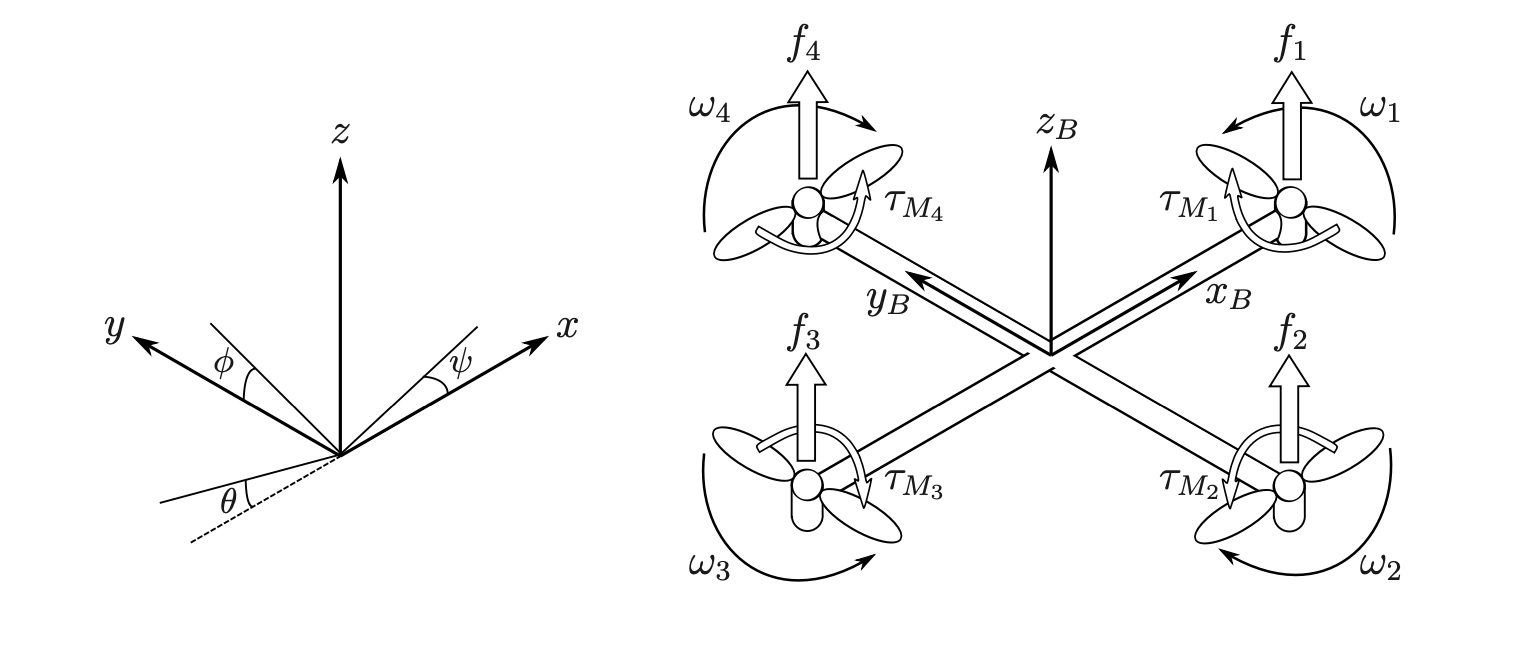
\includegraphics[width=11cm]{01_introduccion/reference_system.png}
\caption{Sistema de referencia inercial y local de un cuadricóptero, recuperado de \cite{luukkonen_2011}.}
\label{fig:interaccion_RL}
\end{figure}

También es necesario considerar la transformación de las velocidades angulares en el sistema de referencia local al inercial que esta dada por la matriz $\mathbf{W}_{\bm{\eta}}$ \cite{capella2020clase}. 
\begin{align}
\begin{bmatrix}
    \dot{\varphi} \\
    \dot{\theta}\\
    \dot{\psi} 
\end{bmatrix}
=
\underbrace{\begin{bmatrix}
    1 & S_{\varphi}T_{\theta} & C_{\varphi}T_{\theta} \\
    0 & C_{\varphi} & -S_{\varphi} \\
    0 & S_{\varphi}/C_{\theta}& C_{\varphi}/C_{\theta}
\end{bmatrix}}_{\mathbf{W}_{\bm{\eta}}}
\begin{bmatrix}
    p \\
    q\\
    r 
\end{bmatrix}.
\label{eq:W_eta}
\end{align}
La expresión $T_{\theta}$ en \ref{eq:W_eta} representa la función $\tan \theta$.

\subsection{Momentos, fuerzas y torques}
Se asumen que el cuadricóptero tiene una estructura simétrica con respecto a los planos $xz$ y $yz$. Por lo que la matriz de momentos de inercia $\mathbf{I}$ es diagonal e $I_{xx} = I_{yy}$. \cite{capella2020clase}
\begin{align}
\mathbf{I} = 
\begin{bmatrix}
    I_{xx} & 0 & 0 \\
    0 & I_{yy} & 0 \\ 
    0 & 0 & I_{zz}
\end{bmatrix}.
\end{align}

Por otro lado la velocidad angular de cada rotor $i$ se denota como $\omega_i$. Cada $\omega_i$ genera una respectiva fuerza $f_i$ en la dirección del eje del rotor, que esta dada por,
$$f_i = k\omega_{i}^2 \quad \forall i \in \{1, 2, 3, 4\}.$$
Dónde $k$ representa el coeficiente de elevación. La acumulación de estas fuerzas genera un empuje $T_{z}$ en la dirección del eje $z$,
$$T_z = \sum_{i=1}^{4}f_i, \quad \mathbf{T}_{B} = 
\begin{bmatrix}
0 \\
0 \\
T_z
\end{bmatrix}.$$

En la dirección de los ángulos en el sistema de referencia local se considera el torque total $\bm{\tau}_{B}$. En particular, este torque total se efectúa sobre los ángulos \textit{roll, pitch} y \textit{yaw}, cuyos componentes estan dados por: $\tau_{\varphi}$, $\tau_{\theta}$ y $\tau_{\psi}$, en el orden correspondiente de los ángulos. \cite{luukkonen_2011}
\begin{align}
    \bm{\tau}_{B} = 
    \begin{bmatrix}
        \tau_{\varphi} \\
        \tau_{\theta} \\
        \tau_{\psi}
    \end{bmatrix}
    = 
    \begin{bmatrix}
        \ell k (\omega_{4}^2 - \omega_2^{2}) \\
        \ell k (\omega_{3}^2 - \omega_1^{2}) \\
        b \sum_{i=1}^{4} (-1)^{i+1} \omega_{i}^2
    \end{bmatrix} 
    \label{eq:torque}
\end{align}

Como se expone en \cite{luukkonen_2011} el movimiento \textit{roll} se obtiene al disminuir la velocidad del segundo rotor e incrementar la del cuarto rotor. Similarmente, el movimiento \textit{pitch} se obtiene al disminuir la velocidad del primer rotor e incrementar la del tercero. El movimiento \textit{yaw} se obtiene al incrementar la velocidad dos rotores opuestos y disminuir la velocidad de los otros dos.
\subsection{Ecuaciones de movimiento}

Bajo esta formulación se considera al cuadricóptero como un sólido rígido \cite{luukkonen_2011}. En este caso se usará las ecuaciones de Newton-Euler para describir la dinámica de traslación y rotación.

En el sistema de referencia local, la fuerza requerida por la aceleración de masa $m\dot{\bm{\upsilon}}$ y la fuerza centrifugal $\bm{\omega} \times(m \bm{\upsilon})$ son iguales a la gravedad $\mathbf{R}^{\top}\mathbf{G}$ y el empuje de los rotores $\mathbf{T}_{B}$ \cite{luukkonen_2011}.
\begin{align}
    m\dot{\bm{\upsilon}} + \bm{\omega} \times (m \bm{\upsilon}) = \mathbf{R}^{\top}\mathbf{G} + \mathbf{T}_{B}, \quad \mathbf{G}
    =
    \begin{bmatrix}
        0 \\
        0 \\
        -g
    \end{bmatrix}.
    \label{eq:u_dynamics}
\end{align}
Al despejar el vector $\dot{\bm{\upsilon}}$ de la expresión \ref{eq:u_dynamics} se obtienen las ecuaciones,
\begin{align}
    \dot u &= rv -qw - g \sin\theta \label{eq:u} \\
    \dot v &= pw -ru -g\cos\theta \cdot \sin\phi \label{eq:v}\\
    \dot w &= qu -pv +g\cos\varphi \cdot \cos\theta-\frac{k}{m} \sum_{i=1}^{4}\omega_i^2 \label{eq:w}.
\end{align}
Las \crefrange{eq:u}{eq:w} representan la dinámica de traslación en el sistema de referencia local.

En el sistema de referencia local, la aceleración angular de los momentos de inercia $\mathbf{I}\dot{\bm{\omega}}$, las fuerzas centrípetas $\bm{\omega} \times (\mathbf{I}\mathbf{\omega})$ es igual al torque total externo $\bm{\tau}_{B}$ \cite{luukkonen_2011}.
\begin{align*}
    \mathbf{I}\dot{\bm{\omega}} + \bm{\omega} \times (\mathbf{I}\bm{\omega}) = \bm{\tau}, 
\end{align*}
si y sólo si,
\begin{align*}
    \dot{\bm{\omega}} = 
    \mathbf{I}^{-1} \left(
        - \begin{bmatrix}
            p \\
            q \\
            r 
        \end{bmatrix}
        \times
        \begin{bmatrix}
            I_{xx} \cdot p \\
            I_{yy} \cdot q \\
            I_{zz} \cdot r
        \end{bmatrix}
        + 
        \begin{bmatrix}
            \tau_{\varphi} \\
            \tau_{\theta} \\
            \tau_{\psi}
        \end{bmatrix}
    \right).
\end{align*}
Realizando las operaciones pertinentes en la expresión $\dot{\bm{\omega}}$ y sustituyendo los términos de torque de \ref{eq:torque} se obtienen lo siguiente,
\begin{align}
\dot p &= \frac{\ell k}{I_{xx}}\left(\omega_4^2 - \omega_2^2\right)-qr \left(\frac{I_{zz} -I_{yy}}{I_{xx}}\right) \label{eq:p}\\
    \dot q &=  \frac{\ell k}{I_{xx}}\left(\omega_3^2 - \omega_1^2\right) - pr \left(\frac{I_{xx} -I_{zz}}{I_{yy}}\right) \label{eq:q}\\
    \dot r &= \frac{b}{I_{zz}}\left(\omega_2^2 + \omega_4^2 - \omega_1^2 - \omega_3^2\right) \label{eq:r}.
\end{align}
Las ecuaciones \crefrange{eq:p}{eq:r} corresponden a la dinámica de rotación en el sistema de referencia local.

Por otra parte la expresión \ref{eq:W_eta}
representa la dinámica de rotación en el sistema de referencia inercial se puede expresar de la siguiente manera,
\begin{align}
    \dot \varphi &= p + (q \sin\varphi + r \cos\varphi) \tan\theta \label{eq:phi}\\
    \dot \theta &= q \cos\varphi - r \sin\varphi \label{eq:theta} \\ 
    \dot \psi &= \left(q \sin\varphi + r \cos\varphi\right) \sec\theta \label{eq:psi}.
\end{align}

Finalmente, la dinámica de traslación en el sistema de referencial inercial se compone por las siguientes expresiones,
\begin{align}
    \dot x &= u \label{eq:x}\\
    \dot y &= v \label{eq:y}\\
    \dot z &= w \label{eq:z}.
\end{align}

En la siguiente tabla se pueden observar los valores constantes de las \crefrange{eq:u}{eq:z}, que fueron recuperados de \cite{fossen_2013}.

\begin{table}[H]
\centering
\begin{tabular}{|c|c|c|c|}
\hline
 \textbf{símbolo}& \textbf{valor} & \textbf{unidad} & \textbf{significado} \\ \hline
 $g$& $9.81$ & $m \cdot s^{-2}$ & constante de gravitación \\ 
 $m$ & $0.468$ & $kg$ & masa del cuadricóptero \\ 
 $\ell$ & $0.225$ & $m$ & distancia entre rotor y centro de masa \\ 
 $b$ & $2.980 \cdot 10^{-6}$ & $-$ & coeficiente de arrastre  \\ 
 $k$& $1.140 \cdot 10^{-7}$ & $-$  & coeficiente de elevación \\ 
 $I_{xx}$& $4.856 \cdot 10^{-3}$ & $kg \cdot m^2$& momento de inercia eje-$x$ \\ 
 $I_{yy}$& $4.856 \cdot 10^{-3}$ & $kg \cdot m^2$& momento de inercia eje-$y$\\ 
 $I_{zz}$& $8.801 \cdot 10^{-3}$ & $kg \cdot m^2$& momento de inercia eje-$z$\\ 
 \hline
\end{tabular}
\label{tab:quadcopter_cons}
\end{table}



\section{Trabajo relacionado}

Para llevar acabo la tarea de controlar un cuadricóptero, durante mucho tiempo han sido ampliamente utilizados métodos convencionales control como \acrfull{pid}, técnicas de control óptimo como \acrfull{ilqr} o estrategias más sofisticadas como \acrfull{mpc}. Sin embargo, estos métodos han mostrado sus limitaciones, por ejemplos los controladores \acrshort{pid} no son autoadaptativos \cite{pang2021}. Los controladores \acrshort{ilqr} y \acrshort{pid} no tienen buen desempeño en sistemas dinámicos no lineales y frecuentemente requieren del conocimiento de un modelo preciso, que puede ser desconocido \cite{pang2021}. La aplicación de \acrshort{mpc} ha demostrado ser computacionalmente costosa \cite{zhang2016}.

Recientemente se ha propuesto utilizar métodos de aprendizaje por refuerzo mediante el entrenamiento de redes neuronales artificiales para resolver este problema de control, debido a que el aprendizaje por refuerzo no requiere de un modelo preciso y puede adaptarse al cambio de condiciones de un entorno. Además, es un método computacionalmente más eficiente que otros algoritmos de control convencionales, como el \acrshort{mpc}, que requieren la predicción de trayectorias del sistema durante su ejecución.  

En el caso de métodos de control del cuadricóptero basados en redes neuronales profundas,  una red neuronal actúa como la política que mapea los estados del cuadricóptero al empuje de cada rotor \cite{hwangbo2017control}. Sin embargo, la aplicación de estos métodos para resolver esta tarea presenta muchos problemas, como son oscilaciones e inestabilidad del cuadricóptero \cite{liu2022robust} o problemas de convergencia del algoritmo de entrenamiento. Debido a esto, se han presentado distintas propuestas que toman en cuenta las características del modelo del cuadricóptero. Existen distintos de métodos basados en \textit{model free} \acrshort{rl}: \cite{liu2022robust}, \cite{Rub2020DeepRL}, \cite{fang-i2019}, \cite{lopes2018intelligent}.

Hwangbo et al. \cite{hwangbo2017control} propusieron un algoritmo que se distingue por su enfoque conservador, pero estable en la regulación del vuelo de un cuadricóptero mediante una red neuronal. Este estudio incorpora un controlador \acrfull{pd} para dirigir el proceso de entrenamiento en sus etapas iniciales. A pesar de que el entrenamiento no contempla la inclusión de un modelo, se destaca la pertinencia de emplear uno para la validación. El controlador resultante demuestra su capacidad para llevar al cuadricóptero desde un estado inicial aleatorio hasta uno deseado.

Anlin et al. \cite{liu2022robust} desarrollaron una estrategia de control robusta para un cuadricóptero un algoritmo de referencia basado en \acrshort{ddpg}.  El método está diseñado para seguir los estados de un modelo de referencia, basado en un modelo de sistema real, y utiliza un sistema de cálculo de recompensas para entrenar al agente de aprendizaje por refuerzo. Este algoritmo mostró mejoras en el rendimiento de vuelo, eliminando errores en estado estacionario, reduciendo la saturación del controlador y garantizando robustez \cite{liu2022robust}.

El potencial del aprendizaje por refuerzo proviene de su habilidad de aprender directamente de un sistema del mundo real \cite{zhang2016}. Sin embargo, este potencial es a su vez una debilidad cuando se aplica sistemas inestables y frágiles \cite{zhang2016}. Un enfoque similar al usado en este trabajo es propuesto en \cite{zhang2016}. Para controlar vehículos aéreos autónomos Zhang et al. \cite{zhang2016} proponen un método que combina un esquema de control óptimo con una  búsqueda guiada de política, mejor conocido por su nombre en inglés \acrfull{gps}. En este método, el \acrshort{gps} es un método transforma un problema de aprendizaje por refuerzo en uno de aprendizaje supervisado, donde un algoritmo de control óptimo provee supervisión para el entrenamiento de una red neuronal artificial, en tanto que, el algoritmo de control óptimo esta orientado a la optimización de trayectorias un algoritmo tipo \acrshort{mpc}. La contribución principal de este enfoque es ofrecer un modelo que imita las capacidades del \acrshort{mpc} a un costo computacional mucho menor, con lo que hace factible su aplicación en situaciones reales \cite{zhang2016}.



\chapter{Teoría de control}
\label{chapter:control_theory}
La teoría de control es el área de las matemáticas aplicadas que estudia los principios en los que se basa el análisis y diseño de sistemas regidos por modelos matemáticos. En este contexto, la acción controlar significa influir en su comportamiento de tal forma que permita alcanzar el objetivo deseado \cite{Sontag1998}. Este campo de estudio permite examinar las características principales de la dinámica de vuelo de un cuadricóptero. Lo cual dará lugar al diseño de estrategias de control con el fin de llevarlo a la posición deseada.

El propósito de este capítulo es  introducir el objeto de estudio de esta área, llamado sistema de control. Posteriormente, se discutirán las características principales de estos sistemas: controlabilidad y estabilidad. Estas características darán pie a examinar estrategias de control, como estabilización por retroalimentación, regulador cuadrático lineal, mejor conocido como \acrfull{lqr} y su versión iterativa llamada \acrfull{ilqr}. Finalmente, se aplica el estudio de teoría de control al sistema dinámico de vuelo de un cuadricóptero y se obtiene una primera estrategia de control.

\section{Sistemas de control}

Los sistemas de control son sistemas dinámicos en tiempo continuo o discreto, que dependen de un parámetro $\mathbf{u}$ \cite{Gruene2021}. Este parámetro puede cambiar con el tiempo o de acuerdo con el estado del sistema. Se puede interpretar a este parámetro como un valor que puede actuar sobre el sistema de forma externa, por ejemplo la aceleración de un vehículo.

En este trabajo tendrán mayor relevancia los sistemas de control invariantes en el tiempo, tanto en tiempo continuo, como discreto. La primera clase de sistemas de control se describen a partir de ecuaciones diferenciales, usualmente ordinarias del tipo,
\begin{align}\label{eq:control_system_con}
    \dot{\mathbf{x}}= f(\mathbf{x}(t), \mathbf{u}(t)).
\end{align}
La variable $t\in \mathbb{R}^{+}$ se interpreta como el tiempo, mientras que $\mathbf{x}(t) \in \mathbb{R}^{n_x}$ y $\mathbf{u}(t)\in \mathbb{R}^{n_u}$ representan las variables de estado y control al tiempo $t$, respectivamente. El mapeo $f:\mathbb{R}^{n_x}\times\mathbb{R}^{n_u}\rightarrow\mathbb{R}^{n_x}$
es el campo vectorial en la \eqreftext{eq:control_system_con}. \cite{Gruene2021}

Análogamente, un sistema de control en tiempo discreto se compone de una ecuación en diferencias, que se expresa de la siguiente manera,
\begin{align}
\label{eq:control_system_dis}
    \mathbf{x}_{k+1}= f(\mathbf{x}_k, \mathbf{u}_k ).
\end{align}
Donde $k\in \mathbb{N}$ es un índice de tiempo discreto. En tanto que $f:\mathbb{R}^{n_x}\times\mathbb{R}^{n_u}\rightarrow\mathbb{R}^{n_x}$ es llamado mapeo o función de transición. \cite{Gruene2021}

\subsection{Sistemas lineales}
El término \textbf{sistema de control lineal} hace referencia a la clase de sistemas dinámicos que describen la relación entre los estados y controles usando ecuaciones diferenciales o ecuaciones en diferencias lineales, según corresponda. Particularmente, la \eqreftext{eq:linear_control_system} muestra una ecuación diferencial lineal para el caso de tiempo continuo, 
\begin{align}\label{eq:linear_control_system}
    \dot{\mathbf{x}} = \mathbf{A}\mathbf{x}+\mathbf{B}\mathbf{u},
\end{align}
donde $\mathbf{A}\in \mathbb{R}^{n_x\times n_x}$ y $ \mathbf{B}\in\mathbb{R}^{n_x\times n_u}$. \cite{Gruene2021}

Los sistemas lineales poseen varias propiedades notables que propician que sean herramientas con múltiples aplicaciones en la vida real. Entre estas propiedades se encuentran: linealidad, controlabilidad y estabilidad. Estos conceptos serán estudiados más adelante. En última instancia estas propiedades permitirán diseñar estrategias de control efectivas.

Un resultado importante es el teorema de existencia y unicidad de los sistemas de control en tiempo continuo. Este teorema no sólo garantiza las propiedades que lleva su nombre, si no que especifica la forma de la solución. Una solución de la \eqreftext{eq:linear_control_system} que satisface la condición inicial $\mathbf{x}(t_0)=\mathbf{x}_0$ está dada por la siguiente expresión,
\begin{align}\label{eq:linear_solution}
    \mathbf{x}(t;t_0, \mathbf{x}_0, \mathbf{u}) &=
    e^{\mathbf{A}(t-t_0)}\mathbf{x}_0 + \int_{t_0}^{t}e^{\mathbf{A}(t-s)}\mathbf{Bu}(s)ds,
\end{align}
donde,
\begin{align}
    e^{t\mathbf{A}} &= \sum^{\infty}_{k=0}\frac{\mathbf{A}^kt^k}{k!}.
\end{align}
En esta instancia $\mathbf{u}\in \mathcal{U}$ es una función continua por partes. \cite{Gruene2021}

\subsection{Linealización de sistemas no lineales}
A diferencia de los sistemas lineales, los sistemas no lineales tienen un comportamiento complejo, lo que hace que el análisis y control de estos sistemas sea desafiante. Sin embargo, en muchos casos es posible obtener una representación lineal de estos sistemas por medio un proceso llamado linealización. Este proceso tiene la finalidad de transformar un sistema no lineal en uno lineal alrededor de una vecindad. Esto simplifica el análisis y el diseño de estrategias de control sobre los sistemas no lineales. Esto se hace, haciendo uso de herramientas proporcionadas por la teoría de sistemas lineales. \cite{capella2020clase}

En una primera etapa se considera la linealización de un sistema de la forma en la \eqreftext{eq:control_system_con} alrededor de un punto fijo. En este caso el proceso consiste en utilizar los términos lineales de la expansión en serie de Taylor alrededor de un punto fijo del propio sistema. Concretamente, para las variables  $(\mathbf{x}, \mathbf{u})$ en una vecindad alrededor del punto fijo $(\mathbf{x}^{*}, \mathbf{u}^{*})$, el sistema dinámico en la \eqreftext{eq:control_system_con} se aproxima linealmente de la siguiente forma,
\begin{align}
    f(\mathbf{x}^{*}+ \overline{\mathbf{x}}, \mathbf{u}^{*}+ \overline{\mathbf{u}}) &\approx f(\mathbf{x}^{*}, \mathbf{u}^{*}) + \nabla_{\mathbf{x}} f(\mathbf{x}^{*}, \mathbf{u}^{*})\cdot \overline{\mathbf{x}}+ \nabla_{\mathbf{u}}f(\mathbf{x}^{*}, \mathbf{u}^{*}) \cdot \overline{\mathbf{u}}, 
    \label{eq:taylor_f}
\end{align}
donde $\overline{\mathbf{x}} = \mathbf{x}-\mathbf{x}^{*}$ y  $\overline{\mathbf{u}} = \mathbf{u} - \mathbf{u}^{*}$ representan un cambio de coordenadas para las variables de estado y control, respectivamente. Debido a que $(\mathbf{x}^{*}, \mathbf{u}^{*})$ es un punto fijo del sistema, se puede establcer $f(\mathbf{x}^{*}, \mathbf{u}^{*})= \mathbf{0}$. De manera que se obtiene la siguiente representación del sistema de control,
\begin{align}\label{eq:taylor_linear_control_system}
    \dot{\mathbf{x}}\approx \underbrace{\mathbf{A}}_{\nabla_{\mathbf{x}} f(\mathbf{x}^{*}, \mathbf{u}^{*})} \overline{\mathbf{x}} + \underbrace{\mathbf{B}}_{\nabla_{\mathbf{u}} f(\mathbf{x}^{*}, \mathbf{u}^{*})}\overline{\mathbf{u}}.
\end{align}

\section{Controlabilidad}
La controlabilidad es la propiedad de un sistema de control que determina si puede alcanzar un estado en particular, empleando una secuencia de control apropiada dentro de una ventana de tiempo especifica. Esta propiedad es fundamental para estudiar los sistema de control. Para describir formalmente está propiedad se recupera la siguiente definición de \cite{Gruene2021}.

\begin{definition}
    Considerando el sistema de control lineal en la \eqreftext{eq:linear_control_system}, un estado $\mathbf{x}_0 \in \mathbb{R}^{n_x}$ se dice que es \textbf{controlable} al estado $\mathbf{x}_1\in \mathbb{R}^{n_x}$ en el tiempo $t_1>0$, si existe $\mathbf{u}\in \mathcal{U}$ tal que 
    \begin{align}
        \mathbf{x}_1 = \mathbf{x}(t_1; \mathbf{x}_0, \mathbf{u}),
    \end{align}
    donde $\mathbf{x}(t_1; \mathbf{x}_0, \mathbf{u})$ representa una solución particular de acuerdo a la \eqreftext{eq:linear_solution}. En este caso, $\mathbf{x}_1$ es llamado estado \textbf{alcanzable} desde $\mathbf{x}_0$ al tiempo $t_1$.
\end{definition}

En el caso de los sistemas de control lineales se tiene una condición para determinar si es un sistema es controlable. Esta condición es conocida como criterio de Kalman y se deriva de una análisis utilizando métodos de álgebra lineal. Este trabajo se limitará a enunciar el criterio recuperado de \cite{Gruene2021} por medio de la siguiente definición y teorema.

\begin{definition}
    La matriz descrita por la siguiente ecuación, 
    $$R(\mathbf{A}, \mathbf{B}) = [\mathbf{B}\ \mathbf{AB}\ \mathbf{A}^2\mathbf{B}\ \cdots\ \mathbf{A}^{n_x-1}\mathbf{B}] \in \mathbb{R}^{n_x \times n_u\cdot n_x},$$ 
    se conoce como la \textbf{matriz de controlabilidad} del sistema en la \eqreftext{eq:linear_control_system}, donde $[\cdot]$ denota la concatenación horizontal (por columnas) de los bloques.
\end{definition}

\begin{theorem}(\textbf{Criterio de Kalman})
    El sistema en la \eqreftext{eq:linear_control_system} es completamente controlable si y sólo si
    $$rango(R(\mathbf{A}, \mathbf{B})) = n_x.$$
    En este caso la pareja de matrices $(\mathbf{A},\mathbf{B})$ se denomina \textbf{controlable}.
\end{theorem} 

\section{Estabilidad}
\label{sec:stability}
La estabilidad es una propiedad fundamental de los sistemas de control, que asegura que la evolución de los estados se mantenga acotada y predecible a lo largo del tiempo. De manera que un análisis sobre la estabilidad permite diseñar estrategias de control efectivas. Antes de abordar el problema de estabilizar un sistema de control, se aclarará matemáticamente el concepto de estabilidad para ecuaciones diferenciales por medio de la siguiente definición retomada de \cite{Gruene2021}.

\begin{definition}
\label{def:stability}
    Considerese el sistema dinámico autónomo, 
$$\dot{\mathbf{x}} = f(\mathbf{x}(t)), \quad \mathbf{x}(0)=\mathbf{x}_0.$$
Supóngase que $f$ tiene un equilibrio en $\mathbf{x}^{*}\in \mathbb{R}^{n_x}$. 
\begin{enumerate}
    \item El equilibrio se denomina \textbf{estable en el sentido de Liapunov}, si para cada $\epsilon> 0$ existe una $\delta>0$ tal que si 
    $$\|\mathbf{x}_0-\mathbf{x}^{*}\|\leq \delta \quad \Rightarrow \quad \|\mathbf{x}(t; \mathbf{x}_0) -\mathbf{x}^{*}\|\leq \epsilon \quad \forall t\geq 0.$$
    \item El equilibrio es llamado \textbf{localmente asintóticamente estable}, si es estable y cumple que 
    $$\lim_{t\rightarrow\infty}\|\mathbf{x}(t;\mathbf{x}_0)-\mathbf{x}^{*}\|=0,$$
    para cualquier $\mathbf{x}_0\in\mathcal{D}$, donde $\mathcal{D}$ es una vecindad abierta de $\mathbf{x}^{*}$. En particular, se le llama \textbf{globalmente asintóticamente estable} si $\mathcal{D}=\mathbb{R}^{n_x}$.
    \item El equilibrio se denomina \textbf{localmente} o \textbf{globalmente exponencialmente estable} si existen las constantes $c, \rho >0$ tales que 
    $$\|\mathbf{x}(t;\mathbf{x}_0)-\mathbf{x}^{*}\| \leq ce^{-\rho t}\|\mathbf{x}_0-\mathbf{x}^{*}\| \quad \forall t\geq 0,$$
    para cualquier $\mathbf{x}_0\in\mathcal{D}$.
\end{enumerate}
\end{definition}

\subsection{Estabilización de sistemas lineales de control}
Los distintos tipos de estabilidad expuestos en la definición 
\ref{def:stability} claramente pueden caracterizar a los sistemas lineales. En este sentido, se pueden estudiar estrategias de control para los sistemas lineales. 

La siguiente definición retoma de lo mostrado en \cite{Gruene2021, capella2020clase}.

\begin{definition}
    Sea el sistema lineal,
    \begin{align}
        \dot{\mathbf{x}}(t) = \mathbf{A}\mathbf{x}(t) + \mathbf{B}\mathbf{u}(t).
        \label{eq:open_linear_system}
    \end{align}
    El \textbf{problema de estabilización por retroalimentación} consiste en encontrar una ley de control de estados $\mu:\mathbb{R}^{n_x}\rightarrow\mathbb{R}^{n_u}$ de la forma
    \begin{align}
        \label{eq:state-feedback}
        \mathbf{u}(t)=\mu(\mathbf{x}(t))=\mathbf{K}\mathbf{x}(t), \qquad \mathbf{K}\in\mathbb{R}^{n_u\times n_x},
    \end{align}
    donde $\mathbf{K}$ se denomina \textbf{ganancia de retroalimentación}. Al sustituir esta ley en el sistema lineal de la ecuación \ref{eq:open_linear_system}, se obtiene el \textbf{sistema de circuito cerrado} descrito por la siguiente ecuación, 
    \begin{align}
    \label{eq:closed-loop}
        \dot{\mathbf{x}}(t) &= (\mathbf{A} + \mathbf{BK})\mathbf{x}(t).
    \end{align}
    El objetivo es elegir $\mathbf{K}$ de modo que el equilibrio $\mathbf{x}^{*}=\mathbf{0}$ del sistema en la \eqreftext{eq:closed-loop} sea asintóticamente estable.
\end{definition}
La dinámica de circuito cerrado está completamente determinada por la matriz,  \begin{align}
(\mathbf{A}+\mathbf{B K}).
\label{eq:matrix_abk}
\end{align}
A su vez la estabilidad del sistema de circuito cerrado así como la tasa de regulación de $\mathbf{x}$ a $\mathbf{0}$ está determinada por los valores propios de la matriz en la \eqreftext{eq:matrix_abk}, que se denotarán por polos del sistema \cite{Kwong2008}. Se puede afirmar que el sistema en la \eqreftext{eq:closed-loop} es asintóticamente estable si y sólo si la parte real de cada valor propio es estrictamente negativa \cite{Gruene2021}. Para regular el sistema en la \eqreftext{eq:closed-loop} usando la \eqreftext{eq:state-feedback}, es necesario determinar que tanto control se tiene sobre los valores propios de la matriz en la \eqreftext{eq:matrix_abk} \cite{Kwong2008}. El problema de encontrar $\mathbf{K}$ tal que permita determinar un conjunto prescrito de valores propios del sistema en la \eqreftext{eq:closed-loop} se llama \textbf{problema de asignación de polos} \cite{Kwong2008}. 

Un resultado importante para los sistemas de control, que fue demostrado en \cite{Kwong2008, Gruene2021}, establece que los polos del circuito cerrado en la \eqreftext{eq:closed-loop} pueden ser arbitrariamente asignados si y sólo si la pareja $(\mathbf{A}, \mathbf{B})$ es controlable. Este resultado es conocido como \textbf{teorema de asignación de polos}. Las implicaciones de este teorema son notables, pues relacionan la controlabilidad y estabilidad, además de permitir diseñar estrategias de control.

\section{Control óptimo}

El área de control óptimo se centra en el estudio del diseño de estrategias de control. Este diseño debe basarse en la optimización de un criterio de desempeño, mientras satisface la restricción impuesta por la dinámica asociada al sistema de control. Existen varias razones por las que este enfoque es bastante potente. En primer lugar permite especificar una meta de control para sistemas de control con distintas características, ya sean sobreactuados, subactuados, lineales, no lineales, deterministas, estocásticos, continuos o discretos. 
En segundo lugar permite describir de manera concisa comportamientos complejos por medio de la definición de la meta a partir de una expresión escalar. Además el control óptimo es adaptable a soluciones numéricas. \cite{underactuated} 

El control óptimo tiene un rol fundamental en la resolución de varios problemas reales. En particular, ha sido ampliamente usado en aplicaciones de la ingeniería donde se desea conseguir el mejor desempeño posible.

Un método de control óptimo extensamente utilizado es el \textbf{regulador cuadrático lineal} o mejor conocido por su nombre en inglés \textbf{\acrfull{lqr}}. Este método en sí es una estrategia de control que explota las capacidades de la teoría de sistemas lineales y la optimización de funciones cuadráticas. 

Esta sección se enfocará en discutir los principios del control óptimo para dar pie al estudio del método \acrshort{lqr} sobre sistemas dinámicos discretos. Posteriormente, se estudiará cómo modificar el método \acrshort{lqr} para utilizarlo en sistemas de control no lineales, como el sistema dinámico que se desea resolver en este trabajo.

\subsection{Planteamiento del problema}
El planteamiento de los problemas de control óptimo discutidos en este trabajo tendrá la particularidad de considerar únicamente problemas para sistemas de control en tiempo discreto de la forma en la \eqreftext{eq:control_system_dis} con horizonte finito.

Bajo las condiciones anteriores, el problema de control óptimo se plantea como la siguiente tarea: dada una condición inicial $\mathbf{x}_{0}\in\mathbb{R}^{n_x}$, encontrar una trayectoria, es decir, una secuencia de pares estado-control $(\mathbf{x}_t, \mathbf{u}_t)$ a lo largo del horizonte temporal, como se muestra en la siguiente ecuación,
\begin{align}
    \bm\tau = \{\mathbf{x}_{0}, \mathbf{u}_0, \mathbf{x}_1, \cdots, \mathbf{x}_{T-1}\mathbf{u}_{T-1}, \mathbf{x}_{T}\},
\end{align}
En este contexto, la variable de control $\mathbf{u}_t\in\mathbb{R}^{n_u}$ también se denotará como \textbf{acción}. De este modo, la tarea consiste en encontrar la sucesión de acciones óptimas que minimice un costo sobre la trayectoria. Dado que la evolución de los estados se determina mediante una función de transición, esto se expresa mediante el siguiente problema de optimización con restricción,
\begin{align}
\min_{\mathbf{u}_0, \mathbf{u}_1, \cdots \mathbf{u}_{T-1}}
\underbrace{\sum_{t=0}^{T} c(\mathbf{x}_t, \mathbf{u}_t)}_{c(\bm\tau)} \quad \text{sujeto a} \quad \mathbf{x}_{t+1}= f(\mathbf{x}_{t}, \mathbf{u}_{t}), \quad \mathbf{x}_{0}\in \mathcal{X}\subset\mathbb{R}^{n_x},
\label{eq:OC_objective}
\end{align}
donde $\mathbf{u}_t \in \mathcal{U}(\mathbf{x}_t)$ para cada tiempo $t\in \{0, \cdots, T-1\}$. En este caso la función $c:\mathcal{X}\times\mathcal{U}\rightarrow\mathbb{R}^{+}$ corresponde al costo instantáneo. En particular, el valor $c(\mathbf{x}_{T}, \mathbf{u}_{T})$ representa el costo final con $\mathbf{u}_{T}=\bm{0}$. Mientras que se representa el costo acumulado de la trayectoria $\bm\tau$ por $c(\bm\tau)$. \cite{underactuated}

De la misma forma se puede expresar explícitamente el objetivo de la optimización como se muestra en la siguiente expresión \cite{underactuated},
\begin{align}
    \min_{\mathbf{u}_0, \mathbf{u}_1, \cdots \mathbf{u}_{T-1}}c(\mathbf{x}_0, \mathbf{u}_0) + c(f(\mathbf{x}_10, \mathbf{u}_0), \mathbf{u}_1) + \cdots + c(f(f\cdots f(\cdots)), 
    \mathbf{u}_{T-1}).
\end{align}
\subsection{Programación dinámica: Iteración de valores}

 Una forma eficiente de resolver esta clase de problemas es por medio de los algoritmos de  programación dinámica.  En general, la \textbf{programación dinámica} hace referencia al conjunto de técnicas que optimizan un programa para resolver un problema secuencial o temporal. Estos métodos parten un problema de alta complejidad en problemas secundarios que se resuelven de forma recursiva \cite{silver2015}. 

Se menciona en \cite{meyn2022} que el problema de control óptimo de estos métodos parte del siguiente hecho: si una pareja de secuencias de estados y acciones dada es óptima y se removiera el primer estado y su respectiva acción, el resto de la secuencia sigue siendo óptima. Este hecho lleva por nombre \textbf{principio de optimalidad de Bellman}.  
Este principio permite interpretar de forma recursiva el objetivo de control óptimo planteado en la \eqreftext{eq:OC_objective} de la siguiente forma,
\begin{equation}
\begin{aligned}
    V_{*}(\mathbf{x}_t) &= 
\min_{\mathbf{u}_t}\left\{ c(\mathbf{x}_t, \mathbf{u}_t) + \min_{\mathbf{u}_{t+1},\cdots, \mathbf{u}_{T-1}}
\sum_{s=t+1}^{T}c(\mathbf{x}_s, \mathbf{u}_s)\right\} \qquad 0 \leq t \leq T-1, \\
&=
\min_{\mathbf{u}_t\in \mathcal{U}(\mathbf{x}_t)} \left\{\underbrace{c(\mathbf{x}_t, \mathbf{u}_t) + V_{*}(\mathbf{x}_{t+1})}_{Q(\mathbf{x}_t, \mathbf{u}_t)}\right\},
\end{aligned}
\label{eq:bellman_eq}     
\end{equation}
donde $\mathbf{x}_{t+1} = f(\mathbf{x}_t, \mathbf{u}_t)$ y $V_{*}(\mathbf{x}_{T})=c(\mathbf{x}_{T+1}, \bm{0})$. Además, la función $Q:\mathcal{X}\times\mathcal{U}\rightarrow\mathbb{R}$, llamada \textbf{función de valor de la acción}, cuantifica el costo inmediato más el costo óptimo futuro asociado a ejecutar la acción $\mathbf{u}_t$ en el estado $\mathbf{x}_t$. La expresión \ref{eq:bellman_eq}, conocida como \textbf{ecuación de Bellman}, se interpreta como una ecuación de punto fijo sobre la función $V_{*}$ \cite{meyn2022}. 

En este contexto la programación dinámica se refiere al uso de algoritmos recursivos para obtener una solución de la ecuación de Bellman \cite{meyn2022}.  

Uno de los métodos más ampliamente utilizados, lleva por nombre \textbf{iteración de valores}. Este algoritmo utiliza el método de aproximaciones sucesivas para resolver la ecuación de punto fijo \ref{eq:bellman_eq} de forma recursiva. Dado un valor inicial $V_0$ la aproximación de $V_{*}$ se realiza usando la siguiente expresión,
\begin{align}
    V_{k+1}(\mathbf{x}) = \min_{\mathbf{u}}\left\{
    c(\mathbf{x}, \mathbf{u})+ V_{k}(f(\mathbf{x}, \mathbf{u}))\right\}\qquad \mathbf{x}\in \mathcal{X}, k\geq 0.
    \label{eq:policy_evaluation}
\end{align}
La \eqreftext{eq:policy_evaluation} permite definir una estrategia para seleccionar acciones óptimas. Dicha estrategia lleva por nombre \textbf{ley de control óptimo} y está dada por,
\begin{align}
    \mu_{k+1}(\mathbf{x}) = \argmin_{u}\left\{
        c(\mathbf{x}, \mathbf{u})+ V_{k}(f(\mathbf{x}, \mathbf{u}))
        \label{eq:policy_update} 
    \right\}.
\end{align}
En general este algoritmo consiste en realizar de forma iterativa los pasos llamados: \textbf{evaluación de política} y \textbf{actualización de política}, que consisten en utilizar las ecuaciones \ref{eq:policy_evaluation} y \ref{eq:policy_update}, respectivamente. 

\subsection{\acrlong{lqr}}
No existe ninguna garantía de que para cualquier sistema de control el método de iteración de valores converja a una solución. No obstante, el método de \acrshort{lqr} garantiza su convergencia valiéndose de los principios de teoría de control en sistemas lineales.
El desarrollo presentado en esta subsección se basa en la formulación clásica descrita en \cite{Bertsekas1995a} y \cite{underactuated}.

Para el uso de este método se establecen las siguientes condiciones. En primer lugar, se considerara un sistema dinámico lineal autónomo de tiempo discreto de la forma,
\begin{align}
    f(\mathbf{x}, \mathbf{u}) = \mathbf{A}\mathbf{x}+ \mathbf{B}\mathbf{u}.
\end{align}
En segundo lugar, se pide un costo cuadrático de la forma,
\begin{align}
c(\mathbf{x}, \mathbf{u}) = \mathbf{x}^{\top}\mathbf{P}\mathbf{x} + \mathbf{u}^{\top}\mathbf{R}\mathbf{u},
\end{align}
donde $\mathbf{P} \in \mathbb{R}^{n_x\times n_x}$ y $\mathbf{R} \in \mathbb{R}^{n_u\times n_u}$ son matrices simétricas positiva semi definida y positiva estrictamente definida, respectivamente. \cite{underactuated}

En este caso la ecuación de Bellman está dada por la siguiente expresión,
\begin{align}
V(\mathbf{x}_{t}) = \min_{
\mathbf{u}}
\left\{    \mathbf{x}_{t}^{\top}\mathbf{P}\mathbf{x}_{t} + \mathbf{u}_{t}^{\top}\mathbf{R}\mathbf{u}_{t} + 
    V(\underbrace{\mathbf{A}\mathbf{x}_{t}+ \mathbf{B}\mathbf{u}_{t}}_{\mathbf{x}_{t+1}})
    \right\}.
    \label{eq:LQR_Bellman}
\end{align}
La solución de la \eqreftext{eq:LQR_Bellman} se obtiene de forma recursiva siguiendo el orden del conjunto $\{T, T-1, \cdots, 1\}$. Para empezar, en el tiempo $t=T+1$ se establece como condición de frontera la siguiente igualdad \cite{underactuated},
\begin{align}
    V(\mathbf{x}_{T}) &= \mathbf{x}_{T}^{\top}\mathbf{P}\mathbf{x}_{T} \qquad \forall \mathbf{x}_{T}\in\mathcal{X}.
    \label{eq:frontier_cond}
\end{align}

 A partir de la condición en la \eqreftext{eq:frontier_cond} se deduce explícitamente la solución a la \eqreftext{eq:LQR_Bellman} y la ley de control óptimo asociada, que están dadas por las siguientes expresiones \cite{Bertsekas1995a},
\begin{align}
    V_{*}(\mathbf{x}_t) &= \mathbf{x}_t^{\top}\mathbf{V}_{t}\mathbf{x}_t, \\
    \mu^{*}(\mathbf{x}_t)&= \mathbf{K}_{t}\mathbf{x}_t,
\end{align}
donde para cada $t \in \{0, 1, \cdots, T-1\}$,
\begin{align}
    \mathbf{K}_t &= - (\mathbf{R}+\mathbf{B}^{\top}\mathbf{V}_{t+1}\mathbf{B})^{-1}\mathbf{B}^{\top}\mathbf{V}_{t+1}\mathbf{A}, \\
    \mathbf{V}_{t} &= \underbrace{\mathbf{Q}}_{\text{costo actual}} + \underbrace{\mathbf{K}_t^{\top}\mathbf{R}\mathbf{K}_t}_{\text{costo de acción $t$}} + 
    \underbrace{(\mathbf{A}+\mathbf{B}\mathbf{K}_{t})^{\top}
    \mathbf{V}_{t+1}
    (\mathbf{A}+\mathbf{B}\mathbf{K}_{t})}_{\text{costo acumulado}}.
\end{align}
En este caso el sistema dinámico descrito como un sistema por retroalimentación mediante la ley de control se expresa de la siguiente manera \cite{underactuated}, 
\begin{align}
    \mathbf{x}_{t+1} = (\mathbf{A} +\mathbf{B}\mathbf{K}_{t})\mathbf{x}_t.
\end{align}

El método de \acrshort{lqr} resulta ser bastante efectivo con sistemas lineales. No obstante, posee varias limitaciones con respecto a una variedad de problemas de la vida real. Entre estas limitaciones se encuentra que problemas de control (como el que se plantea en este trabajo) están representados por sistemas no lineales. A pesar de que se puede utilizar una aproximación lineal del sistema, esto sólo es efectivo en regiones pequeñas. Otra limitación importante, es que restringe la forma que debe tener la función de costo. 

\subsection{\acrlong{ilqr}}\label{sub_sec:iLQR}

Para superar los retos discutidos anteriormente, se introduce el método conocido como \textbf{regulador cuadrático lineal iterativo} o \textbf{\acrfull{ilqr}}. Este método hereda las capacidades del algoritmo \acrshort{lqr} para aplicarlos sobre un sistema no lineal y una función de costo diferenciable. 

Este algoritmo en lugar de usar la dinámica dada por un sistema lineal, construye una aproximación lineal variable en el tiempo de la dinámica correspondiente a un sistema no lineal. De manera similar, remplaza la representación cuadrática de un costo por una aproximación cuadrática variable en el tiempo de una función de costo más general. Esta capacidad de capturar la no linealidad del sistema permite diseñar controles más efectivos y con mejores resultados. \cite{berkeley2017deeprl}

Para lograr obtener las representaciones aproximadas de la dinámica y el costo, será necesario establecer ciertas hipótesis. Para empezar el sistema dinámico $f$ debe  de ser diferenciable, es decir, que $f\in\mathcal{C}^{1}(\mathcal{X}\times\mathcal{U}, \mathcal{X})$. Por otra parte el costo $c$ se asume que por lo menos es una función doblemente diferenciable, lo que quiere decir que $c \in \mathcal{C}^{2}\left(\mathcal{X}\times\mathcal{U}, \mathbb{R}^{+}\right)$.  

La siguiente descripción del algoritmo \acrshort{ilqr} está basada en el curso \textit{CS 294: Deep Reinforcement Learning, Fall 2017} de la universidad de Berkeley \cite{berkeley2017deeprl, hui2018rl}.

\subsubsection{Estabilización de trayectorias locales para sistemas no lineales}
El método requiere una trayectoria factible de estados y acciones para resolver de forma iterativa el problema en la \eqreftext{eq:OC_objective}. A esta secuencia de referencia inicial se le denomina \textbf{trayectoria nominal} y se representa mediante la expresión,
\begin{align}
\hat{\bm\tau} = \left\{\hat{\mathbf{x}}_0, \hat{\mathbf{u}}_0, \hat{\mathbf{x}}_1, \hat{\mathbf{u}}_1\cdots, \hat{\mathbf{x}}_{T-1}, \hat{\mathbf{u}}_{T-1}, \hat{\mathbf{x}}_{T} \right\},    
\label{eq:nominal_traj}
\end{align}
A partir de la trayectoria $\hat{\bm\tau}$ en cada paso de tiempo se construye un nuevo sistema de coordenadas. Concretamente, para cada $t \in \{0, \cdots, T-1\}$, las variables de estado y control están dadas por las siguiente expresiones,
\begin{align}
    \bar{\mathbf{x}}_t = \mathbf{x}_t - \hat{\mathbf{x}}_t, \qquad \bar{\mathbf{u}}_t = \mathbf{u}_t - \hat{\mathbf{u}}_t.
\end{align}
Estas nuevas coordenadas serán útiles para obtener una aproximación lineal del sistema dinámico $f$. Específicamente esta aproximación se realiza calculando el polinomio de Taylor de grado uno para $f$. Este cálculo se realiza alrededor de cada pareja estado-acción de $\hat{\bm{\tau}}$, como se muestra en la siguiente expresión \cite{underactuated},
\begin{equation}
    \begin{aligned}
    \bar{\mathbf{x}}_{t+1} &= \mathbf{x}_{t+1} - \hat{\mathbf{x}}_{t+1} = f(\mathbf{x}_t, \mathbf{u}_t) - f(\hat{\mathbf{x}}_t, \hat{\mathbf{u}}_{t}) \\
    &\approx f(\hat{\mathbf{x}}_t, \hat{\mathbf{u}}_t) + \underbrace{\nabla_{\mathbf{x}} f(\hat{\mathbf{x}}_t, \hat{\mathbf{u}}_t)}_{\mathbf{A}_t}(\mathbf{x}_t - \hat{\mathbf{x}}_t) + \underbrace{\nabla_{\mathbf{u}} f(\hat{\mathbf{x}}_t, \hat{\mathbf{u}}_t)}_{\mathbf{B}_t} (\mathbf{u}_t - \hat{\mathbf{u}}_t) -f(\hat{\mathbf{x}}_t, \hat{\mathbf{u}}_t) \\
    & \approx \mathbf{A}_t \bar{\mathbf{x}}_t + \mathbf{B}_t \bar{\mathbf{u}}_t \\
    & \approx \mathbf{F}_{t} 
    \begin{bmatrix}
        \bar{\mathbf{x}}_t \\
        \bar{\mathbf{u}}_t
    \end{bmatrix}\qquad t\in \{0, \cdots, T-1\}.
    \end{aligned}
    \label{eq:taylor_control_system}
\end{equation} 

La \eqreftext{eq:taylor_control_system} se asemeja a la representación del sistema de control utilizada para el método \acrshort{lqr}. Sin embargo, esta expresión representa un sistema de control no autónomo en tiempo discreto. La linealización varía con respecto a la evolución del tiempo y no se hace específicamente sobre un punto fijo del sistema. Esta linealización es valida para cualquier trayectoria factible. Esta representación permitirá tener las propiedades de un sistema lineal, mientras que la región de estabilidad es más grande. \cite{underactuated} 

Para obtener una aproximación cuadrática del costo $c$, se calcula el polinomio de Taylor de grado dos, alrededor de los elementos de $\bm\tau$, como se muestra la siguiente expresión,
\begin{equation}
\begin{aligned}
    c(\mathbf{x}_t, \mathbf{u}_t) \approx& 
    c\left(\hat{\mathbf{x}}_t, \hat{\mathbf{u}}_t\right) 
    + 
\underbrace{\nabla_{\mathbf{x}\mathbf{u}}
    c\left(\hat{\mathbf{x}}_t, \hat{\mathbf{u}}_t\right)}_{\mathbf{c}_t}
    \begin{bmatrix}
        \mathbf{x}_t - \hat{\mathbf{x}}_t \\
        \mathbf{u}_t - \hat{\mathbf{u}}_t
    \end{bmatrix}
    + \frac{1}{2}
    \begin{bmatrix}
        \mathbf{x}_t - \hat{\mathbf{x}}_t \\
        \mathbf{u}_t - \hat{\mathbf{u}}_t
    \end{bmatrix}^{\top}
    \underbrace{\nabla_{\mathbf{x}\mathbf{u}}^{2} 
    c\left(\hat{\mathbf{x}}_t, \hat{\mathbf{u}}_t\right)}_{\mathbf{C}_t}
    \begin{bmatrix}
        \mathbf{x}_t - \hat{\mathbf{x}}_t \\
        \mathbf{u}_t - \hat{\mathbf{u}}_t
    \end{bmatrix} \\
=& \text{ C} + \frac{1}{2} 
\begin{bmatrix}
        \bar{\mathbf{x}}_t \\
        \bar{\mathbf{u}}_t
    \end{bmatrix}^{\top}
    \mathbf{C}_t 
    \begin{bmatrix}
        \bar{\mathbf{x}}_t \\
        \bar{\mathbf{u}}_t
    \end{bmatrix}
    + 
    \begin{bmatrix}
        \bar{\mathbf{x}}_t \\
        \bar{\mathbf{u}}_t
    \end{bmatrix}^{\top}
    \mathbf{c}_t ,
\end{aligned}
    \label{eq:taylor_cost}
\end{equation}
donde $C\in\mathbb{R}$ es una constante.

Se usará la representación del costo dada por la \eqreftext{eq:taylor_cost}. En este caso la matriz $\mathbf{C}_{t}$ y el vector $\mathbf{c}_t$ representan el hessiano y el gradiente evaluados en cada estado-acción de $\bm{\tau}$, respectivamente. Con la intención de tener expresiones más simples, se parte la matriz $\mathbf{C}_t$ y el vector $\mathbf{c}_t$ en componentes, como se muestra en la siguiente expresión, 
\begin{align}
\mathbf{C}_t =
    \begin{bmatrix}
     \mathbf{C}_{\mathbf{x}\mathbf{x}_t}& \rvline & \mathbf{C}_{\mathbf{x} \mathbf{u}_t} \\ \hline 
    \mathbf{C}_{\mathbf{u}\mathbf{x}_t} & \rvline & 
    \mathbf{C}_{\mathbf{u}\mathbf{u}_t} 
    \end{bmatrix} 
    \in \mathbb{R}^{(n_{x}+n_{u})\times(n_{x} + n_{u})}
    ,
    \quad 
    \mathbf{c}_t = 
    \begin{bmatrix}
        \mathbf{c}_{\mathbf{x}_t} \\
        \mathbf{c}_{\mathbf{u}_t}
    \end{bmatrix} 
    \in \mathbb{R}^{n_x + n_u}
    \qquad t\in \{0, \cdots, T-1\}.
\end{align} 
\subsubsection{\textit{Backward pass}}
Al igual que en el algoritmo \acrshort{lqr}, este método resuelve la ecuación de Bellman de forma recursiva. En este caso se establece la siguiente condición de frontera,
\begin{align}\label{eq:Q_front}
    Q(\mathbf{x}_{T-1}, \mathbf{u}_{T-1}) = c(\mathbf{x}_{T-1}, \mathbf{u}_{T-1}) \quad \forall\mathbf{x}_{T-1} \in\mathcal{X}, \mathbf{u}_{T-1} \in \mathcal{U},
\end{align}
donde, como se indicó anteriormente, $\mathcal{X}$ y $\mathcal{U}$ representan los conjuntos de estados y de variables de control, respectivamente.

En este caso se usa la forma cuadrática del costo para la igualdad en la \eqreftext{eq:Q_front}. Si se asume que la matriz $\mathbf{C}_{T-1}$ es positiva definida, es posible encontrar la función de valor óptima. A partir de resolver la ecuación $\nabla_{\mathbf{u}_{T-1}}Q(\mathbf{x}_{T-1}, \mathbf{u}_{T-1})=0$ para la variable $\mathbf{u}_{T-1}$, como se muestra en la siguiente expresión,
\begin{equation}
    \begin{aligned}
       0 &= \mathbf{C}_{\mathbf{u}\mathbf{x}_{T-1}}\bar{\mathbf{x}}_{T-1}
    + \mathbf{C}_{\mathbf{u}\mathbf{u}_{T-1}}\bar{\mathbf{u}}_{T-1}
    + \mathbf{c}_{\mathbf{u}_{T-1}}, \\
    \iff \bar{\mathbf{u}}_{T-1} &= -\mathbf{C}_{\mathbf{u}\mathbf{u}_{T-1}}^{-1}(\mathbf{C}_{\mathbf{u}\mathbf{x}_{T-1}}\bar{\mathbf{x}}_{T-1} + \mathbf{c}_{\mathbf{u}_{T-1}}), \\
    \iff \mathbf{u}_{T-1} &= \hat{\mathbf{u}}_{T-1} + \mathbf{K}_{T-1}(\mathbf{x}_{T-1} - \hat{\mathbf{x}}_{T-1}) + \mathbf{k}_{T-1},
    \end{aligned}
\end{equation}
donde, 
\begin{align}
    \mathbf{K}_{T-1} = -\textbf{C}_{\mathbf{u} \mathbf{u}_{T-1}}^{-1}\mathbf{C}_{\mathbf{u}\mathbf{x}_{T-1}}, \quad \mathbf{k}_{T-1}= -\mathbf{C}_{\mathbf{u} \mathbf{u}_{T-1}}^{-1}\mathbf{c}_{\mathbf{u}_{T-1}}.
\end{align} 

Una vez teniendo el valor óptimo $\textbf{u}_{T-1}$
se calcula la función de valor óptima para el paso $t=T-1$,
\begin{equation}
    \begin{aligned}
    V(\mathbf{x}_{T-1}) &= \min_{\mathbf{u}_{T-1}}Q(\mathbf{x}_{T-1}, \mathbf{u}_{T-1}) \\
    &= \text{ C} + \frac{1}{2}
    \begin{bmatrix}
        \bar{\mathbf{x}}_{T-1} \\
        \mathbf{K}_{T-1}\bar{\mathbf{x}}_{T-1} + \mathbf{k}_{T-1}
    \end{bmatrix}^{\top}
    \mathbf{C}_{T-1} 
    \begin{bmatrix}
        \bar{\mathbf{x}}_{T-1} \\
        \mathbf{K}_{T-1}\bar{\mathbf{x}}_{T-1} + \mathbf{k}_{T-1}
    \end{bmatrix}
    + 
    \begin{bmatrix}
        \bar{\mathbf{x}}_{T-1} \\
        \mathbf{K}_{T-1}\bar{\mathbf{x}}_{T-1} + \mathbf{k}_{T-1}
    \end{bmatrix}^{\top}
    \mathbf{c}_{T-1} \\
    &= \text{ C} + 
    \frac{1}{2}\bar{\mathbf{x}}_{T-1} \mathbf{C}_{\mathbf{x}\mathbf{x}_{T-1}}
    \bar{\mathbf{x}}_{T-1}  
    + \frac{1}{2}\bar{\mathbf{x}}_{T-1}^{\top}
    \mathbf{C}_{\mathbf{x}\mathbf{u}_{T-1}}
    \mathbf{K}_{T-1}
    \bar{\mathbf{x}}_{T-1} 
     +
    \frac{1}{2}
    \bar{\mathbf{x}}_{T-1}^{\top}
    \mathbf{K}_{T-1}^{\top}
    \mathbf{C}_{\mathbf{u}\mathbf{x}_{T-1}} 
    \bar{\mathbf{x}}_{T-1} \\
    & + \frac{1}{2}
    \bar{\mathbf{x}}_{T-1}^{\top}
    \mathbf{K}_{T-1}^{\top}
    \mathbf{C}_{\mathbf{u}\mathbf{u}_{T-1}}\mathbf{K}_{T-1}
    \bar{\mathbf{x}}_{T-1} 
    + 
    \bar{\mathbf{x}}_{T-1}^{\top}
    \mathbf{K}_{T-1}^{\top} 
    \mathbf{C}_{\mathbf{u}\mathbf{u}_{T-1}}
    \mathbf{k}_{T-1} 
    + 
    \frac{1}{2} 
    \bar{\mathbf{x}}_{T-1}^{\top}
    \mathbf{C}_{\mathbf{x}\mathbf{u}_{T-1}}\mathbf{k}_{T-1} \\
    &+ \bar{\mathbf{x}}_{T-1}^{\top}
    \mathbf{c}_{\mathbf{x}_{T-1}} + 
    \bar{\mathbf{x}}^{\top}_{T-1}
    \mathbf{K}_{T-1}^{\top}
    \mathbf{c}_{\mathbf{u}_{T-1}} \\
    &= \text{ C} + \frac{1}{2}\bar{\mathbf{x}}_{T-1}^{\top} \mathbf{V}_{T-1}\bar{\mathbf{x}}_{T-1} + \bar{\mathbf{x}}_{T-1}^{\top} \mathbf{v}_{T-1},
    \end{aligned}
    \label{eq:ilqr_VT}
\end{equation}
donde,
\begin{align}
    \mathbf{V}_{T-1} &= \mathbf{C}_{\mathbf{x}\mathbf{x}_{T-1}} 
    + \mathbf{C}_{\mathbf{xu}_{T-1}} 
    \mathbf{K}_{T-1}^{\top} 
    \mathbf{C}_{\mathbf{ux}_{T-1}}
    + \mathbf{K}_{T-1}^{\top}\mathbf{C}_{\mathbf{uu}_{T-1}}
    \mathbf{K}_{T-1}, \\
    \mathbf{v}_{T-1} &= \mathbf{c}_{\mathbf{x}_{T-1}} 
    + \mathbf{C}_{\mathbf{xu}_{T-1}}\mathbf{k}_{T-1} 
    + \mathbf{K}_{T-1}^{\top} \mathbf{C}_{\mathbf{u}_{T-1}} 
    + \mathbf{K}_{T-1}^{\top} \mathbf{C}_{\mathbf{uu}_{T-1}}\mathbf{k}_{T-1}.
\end{align}

Una vez resuelta la ecuación de Bellman para el paso $T-1$, se puede resolver dicha ecuación para el paso $T-2$,
\begin{align} \label{eq:Q_T_1}
    Q(\mathbf{x}_{T-2}, \mathbf{u}_{T-2})
    &= \text{ C} 
    +\frac{1}{2}
    \begin{bmatrix}
        \bar{\mathbf{x}}_{T-2} \\
        \bar{\mathbf{u}}_{T-2}
    \end{bmatrix}^{\top}
    \mathbf{C}_{T-2}
    \begin{bmatrix}
        \bar{\mathbf{x}}_{T-2} \\
        \bar{\mathbf{u}}_{T-2}
    \end{bmatrix}
    + 
    \begin{bmatrix}
        \bar{\mathbf{x}}_{T-2} \\
        \bar{\mathbf{u}}_{T-2}
    \end{bmatrix}^{\top}
    \mathbf{c}_{T-2}
    +
    V(\mathbf{x}_{T-1}),
\end{align}
donde la función $V(\mathbf{x}_{T-1})$ está dada por la \eqreftext{eq:ilqr_VT}. Sustituyendo $\bar{\mathbf{x}}_{T-1}$ por el lado derecho de la \eqreftext{eq:taylor_control_system} para $t=T-2$, se obtiene que, 
\begin{align}
    V(\mathbf{x}_{T-1}) &= \text{ C} 
    + \frac{1}{2}
    \begin{bmatrix}
        \bar{\mathbf{x}}_{T-2}\\
        \bar{\mathbf{u}}_{T-2}
    \end{bmatrix}^{\top}
    \mathbf{F}_{T-2}^{\top} \mathbf{V}_{T-1}
    \mathbf{F}_{T-2}
    \begin{bmatrix}
        \bar{\mathbf{x}}_{T-2}\\
        \bar{\mathbf{u}}_{T-2}
    \end{bmatrix}
    + 
    \begin{bmatrix}
        \bar{\mathbf{x}}_{T-2}\\
        \bar{\mathbf{u}}_{T-2}
    \end{bmatrix}^{\top}
    \mathbf{F}_{T-2}^{\top} 
    \mathbf{v}_{T-1}.
\end{align}
Esta modificación, permite reordenar la \eqreftext{eq:Q_T_1} de la siguiente forma,
\begin{align}
    Q(\mathbf{x}_{T-2}, \mathbf{u}_{T-2}) &= 
    \text{ C} 
    + \frac{1}{2} 
    \begin{bmatrix}
        \bar{\mathbf{x}}_{T-2} \\
        \bar{\mathbf{u}}_{T-2}
    \end{bmatrix}^{\top}
    \mathbf{Q}_{T-2} 
    \begin{bmatrix}
        \bar{\mathbf{x}}_{T-2} \\
        \bar{\mathbf{u}}_{T-2}
    \end{bmatrix}
    +
    \begin{bmatrix}
        \bar{\mathbf{x}}_{T-2} \\
        \bar{\mathbf{u}}_{T-2}
    \end{bmatrix}^{\top}
    \mathbf{q}_{T-2},
\end{align}
donde,
\begin{align}
    \mathbf{Q}_{T-2} &= \mathbf{C}_{T-2} 
    + \mathbf{F}_{T-2}^{\top}\mathbf{V}_{T-1}
    \mathbf{F}_{T-2}, \\
    \mathbf{q}_{T-2} &= \mathbf{c}_{T-2} 
    + \mathbf{F}_{T-2}^{\top}\mathbf{v}_{T-1}.
\end{align}

Estos cambios permiten obtener la ley de control óptima para el paso $t=T-2$ por medio de solución de la ecuación $\nabla_{\mathbf{u}}Q(\mathbf{x}_{T-2}, \mathbf{u}_{T-2})= \mathbf{0}$, como se muestra a continuación,
\begin{equation}
    \begin{aligned}
    \bm{0} &= \mathbf{Q}_{\mathbf{ux}_{T-2}}
    \bar{\mathbf{x}}_{T-2} + \mathbf{Q}_{\mathbf{uu}_{T-2}} \bar{\mathbf{u}}_{T-2}
    + \mathbf{q}_{\mathbf{u}_{T-2}} \\
    \iff \bar{\mathbf{u}}_{T-2} &= 
    -\textbf{Q}_{\mathbf{u} \mathbf{u}_{T-2}}^{-1}\mathbf{Q}_{\mathbf{u}\mathbf{x}_{T-2}} \bar{\mathbf{x}}_{T-2}+ \mathbf{Q}_{\mathbf{u} \mathbf{u}_{T-2}}^{-1}\mathbf{q}_{\mathbf{u}_{T-2}}  \\
    \iff \mathbf{u}_{T-2} &= \hat{\mathbf{u}}_{T-2}
    + \mathbf{K}_{T-2} (\mathbf{x}_{T-2}-\hat{\mathbf{x}}_{T-2})+ \mathbf{k}_{T-2},
    \end{aligned}
\end{equation}
donde,
\begin{align}
    \mathbf{K}_{T-2} = -\textbf{Q}_{\mathbf{u} \mathbf{u}_{T-2}}^{-1}\mathbf{Q}_{\mathbf{u}\mathbf{x}_{T-2}}, \quad \mathbf{k}_{T-2}= -\mathbf{Q}_{\mathbf{u} \mathbf{u}_{T-2}}^{-1}\mathbf{q}_{\mathbf{u}_{T-2}}.
\end{align}
Este cálculo permite, a su vez definir la función de valor óptima para el paso $t=T-2$ de la forma, 
\begin{align}
    V(\mathbf{x}_{T-2}) = \text{ C} 
    + \frac{1}{2}\bar{\mathbf{x}}_{T-2}^{\top}
    \mathbf{V}_{T-2}
    \bar{\mathbf{x}}_{T-2}
    + 
    \bar{\mathbf{x}}_{T-2}^{\top}
    \mathbf{v}_{T-2},
\end{align}
donde,
\begin{align}
    \mathbf{V}_{T-2} &= \mathbf{Q}_{\mathbf{xx}_{T-2}}
    + \mathbf{Q}_{\mathbf{xu}_{T-2}}\mathbf{K}_{T-2}
    + \mathbf{K}_{T-2}^{\top}\mathbf{Q}_{\mathbf{ux}_{T-1}}
    + \mathbf{K}_{T-2}^{\top}\mathbf{C}_{\mathbf{uu}_{T-2}}\mathbf{K}_{T-2}, \\
    \mathbf{v}_{T-1} &= \mathbf{q}_{\mathbf{x}_{T-2}}
    + \mathbf{C}_{\mathbf{xu}_{T-2}}\mathbf{k}_{T-2}
    +\mathbf{K}_{T-2}^{\top}\mathbf{C}_{\mathbf{u}_{T-2}}
    + \mathbf{K}_{T-2}^{\top}\mathbf{C}_{\mathbf{uu}_{T-2}}\mathbf{k}_{T-2}.
\end{align}

A partir de los cálculos anteriores se puede obtener inductivamente la ley de control óptimo para cualquier paso de tiempo $t<T-1$ como, 
\begin{align} \label{eq:control_law}
    \mu(\mathbf{x}_t) := \mathbf{u}_t = \hat{\mathbf{u}}_t + \mathbf{K}_t(\hat{\mathbf{x}}_t-\mathbf{x}_t) + \mathbf{k}_t,
\end{align}
donde,
\begin{align}
\mathbf{K}_{t} = -\mathbf{Q}_{\mathbf{uu}_t}^{-1}\mathbf{Q}_{\mathbf{ux}_t}, \quad \mathbf{k}_{t} = \mathbf{Q}_{\mathbf{uu}_t}^{-1} \mathbf{q}_{\mathbf{u}_t}.
\end{align}
Aquí, $\mathbf{K}_{t}$ corresponde a la ganancia de realimentación al tiempo $t$ y $\mathbf{k}_{t}$ al término aditivo de la ley de control al tiempo $t$.
Así mismo, se puede definir la función de valor óptima, dada por la siguiente expresión,
\begin{align}
    V(\mathbf{x}_{t}) = \text{ C} 
    + \frac{1}{2}\bar{\mathbf{x}}_{t}^{\top}
    \mathbf{V}_{t}
    \bar{\mathbf{x}}_{t}
    + 
    \bar{\mathbf{x}}_{t}^{\top}
    \mathbf{v}_{t},
\end{align}
donde,
\begin{align}
    \mathbf{V}_{t} &= \mathbf{Q}_{\mathbf{xx}_{t}}
    + \mathbf{Q}_{\mathbf{xu}_{t}}\mathbf{K}_{t}
    + \mathbf{K}_{t}^{\top}\mathbf{Q}_{\mathbf{ux}_t}
    + \mathbf{K}_{t}^{\top}\mathbf{C}_{\mathbf{uu}_t}\mathbf{K}_{t}, \\
    \mathbf{v}_{t} &= \mathbf{q}_{\mathbf{x}_{t}}
    + \mathbf{C}_{\mathbf{xu}_{t}}\mathbf{k}_{t}
    +\mathbf{K}_{t}^{\top}\mathbf{C}_{\mathbf{u}_{t}}
    + \mathbf{K}_{t}^{\top}\mathbf{C}_{\mathbf{uu}_{t}}\mathbf{k}_{t}.
\end{align}
\subsubsection{\textit{Forward pass}}
Una vez calculada la ley de control óptimo en la \eqreftext{eq:control_law}, se puede obtener una nueva trayectoria factible $\hat{\bm\tau}$ de la siguiente manera,
\begin{align}
    \hat{\mathbf{x}}_0 &= \mathbf{x}_0, \\
    \hat{\mathbf{u}}_t &= \mu(\mathbf{x}_t), \quad \hat{\mathbf{x}}_{t+1} =f(\hat{\mathbf{x}}_t, \hat{\mathbf{u}}_t)\quad\forall t \in \{0, \cdots T-1\} .
\end{align}

\subsubsection{Búsqueda de Línea}
A diferencia de los sistemas cuadráticos lineales para los sistemas no lineales no se puede obtener la solución exacta de la \eqreftext{eq:control_law} después de una sola iteración. Además para este último tipo de sistemas, cuando la nueva trayectoria se aleja demasiado de la región de validez del modelo, el costo puede no disminuir y esto puede ocasionar una divergencia \cite{Tassa2012}. En \cite{Tassa2012} se propone incorporar un parámetro de búsqueda en línea $\alpha \in \bm{\alpha}$, con el conjunto de candidatos dado por, 
\begin{align}
\bm{\alpha} = \left\{\left(\frac{1}{2}\right)^i\right\}_{i=0}^{7}.
\end{align}
Con ello, la ley de control se actualiza de la siguiente forma,
\begin{align} \label{eq:control_law_alpha}
    \mu(\mathbf{x}_t) := \mathbf{u}_t = \hat{\mathbf{u}}_t + \mathbf{K}_t(\hat{\mathbf{x}}_t-\mathbf{x}_t) + \alpha\mathbf{k}_t,
\end{align}
Entonces se realizan varias iteraciones del método de \acrshort{ilqr}, incrementando progresivamente el valor de $\alpha$ en cada iteración dentro del conjunto $\bm{\alpha}$. Este proceso se detiene cuando se cumple la siguiente condición \cite{ilqr2019}, 
\begin{align}
\label{eq:cost_thershold}
    \frac{|c(\bm\tau)-c\left(\hat{\bm\tau}\right)|}{c\left(\hat{\bm\tau}\right)} < \epsilon_{tol},
\end{align}
donde $c(\hat{\bm\tau})$, $c(\bm\tau)$ representan el costo resultante de la optimización en la iteración más reciente y el costo de la iteración anterior, respectivamente. En este caso $\epsilon_{tol}\in\mathbb{R}^{+}$ es un umbral determinado de convergencia.

\subsubsection{Regularización} 
En general el hessiano $\mathbf{C}_t$ no es una matriz positiva definida en cada paso de tiempo $t$, pues el costo $c(\mathbf{x}_t, \mathbf{u}_t)$ no necesariamente es una función convexa globalmente. Para atender esta situación se propuso en \cite{ilqr2019} el siguiente esquema de regularización, 
\begin{align}
    \tilde{\mathbf{Q}}_{\mathbf{uu}_t} &= \mathbf{C}_{\mathbf{uu}_t} + \mathbf{F}_{\mathbf{u}_t}^{\top}(\mathbf{V}_t + \lambda \mathbf{I}_{n_x})
    \mathbf{F}_{\mathbf{u}_t}, \\
    \tilde{\mathbf{Q}}_{\mathbf{ux}_t} &= 
    \mathbf{C}_{\mathbf{ux}_t} + \mathbf{F}_{\mathbf{u}_t}^{\top}(\mathbf{V}_t + \lambda \mathbf{I}_{n_x})
    \mathbf{F}_{\mathbf{x}_t}, \\
    \mathbf{K}_{t} &= -\tilde{\mathbf{Q}}_{\mathbf{uu}_t}^{-1}\tilde{\mathbf{Q}}_{\mathbf{ux}_t}, \\
    \mathbf{k}_{t} &= \tilde{\mathbf{Q}}_{\mathbf{uu}_t}^{-1} \tilde{\mathbf{q}}_{\mathbf{u}_t}, 
\end{align}
donde $\lambda$ es un parámetro de regularización. Este esquema es una versión de primer orden basado en el que fue propuesto en \cite{Tassa2012}. 

La actualización del parámetro $\lambda$ es de vital importancia debido a las siguientes tres circunstancias. La primera circunstancia se da si se está cerca del mínimo, en este caso se desea que el valor $\lambda$ se acerque los más rápido posible a $0$. En el caso en que el la matriz $\tilde{\mathbf{Q}}_{uu}$ no sea positiva definida, se desea que el valor de $\lambda$ incremente rápidamente. Finalmente, si se requiere algún valor $\lambda > 0$, se desea ajustarlo con precisión para que esté lo más cerca posible del valor mínimo, pero no más pequeño. Para lidiar adecuadamente con estos casos, se usa el siguiente régimen de actualización de $\lambda$. \cite{Tassa2012}
\begin{enumerate}
    \item Para incrementar $\lambda$,
    \begin{align}
        \Delta^{(k +1)} = \max(\Delta_0, \Delta^{(k)}\cdot \Delta_0), \qquad \lambda^{(k+1)} = \max(\lambda_{\min}, \mu^{(k)}\cdot\Delta^{(k+1)}).
        \label{eq:lamb_increase}
    \end{align}
    \item Para disminuir $\lambda$,
    \begin{align}
         \Delta^{(k+1)} = \min\left(
    \frac{1}{\Delta_0}, \frac{\Delta^{(k)}}{\Delta_0}
    \right),
    \qquad
        \lambda^{(k+1)} = 
    \begin{cases}
        \lambda^{(k)} \cdot \Delta^{(k+1)} &\text{si } \lambda^{(k)} \cdot \Delta^{(k+1)} > \lambda_{\min} \\
        0 &\text{e.o.c}
    \end{cases}.
    \label{eq:lamb_decrease}
    \end{align}
\end{enumerate}
Donde $\Delta^{k}$ representa el $k$-ésimo incremento del factor de ajuste de regularización y $\Delta_{0}$ su valor inicial. Asimismo, $\lambda_{\min}$ y $\lambda_{\max}$ corresponden a los valores mínimo y máximo del parámetro de regularización, mientras que $\lambda_0$ es su valor inicial. En este trabajo se emplean los valores $\Delta_{0}=2$, $\lambda_0=20$, $\lambda_{\min}=10^{-3}$ y $\lambda_{\max}=10^4$, tomados de \cite{Tassa2012}.

Este método es una aproximación al método de Newton para optimizar la \eqreftext{eq:OC_objective}, ya que \acrshort{ilqr} sigue la misma idea de aproximar localmente funciones no lineales a partir de su expansión en serie de Taylor \cite{levine2017}.

El procedimiento principal de \acrshort{ilqr} se resume en el algoritmo \ref{alg:ilqr}, el cual emplea el método de búsqueda de línea descrito en el algoritmo \ref{alg:line_search}.

\begin{algorithm}[H]
\caption{Regularización y Búsqueda de línea \acrshort{ilqr}}
\label{alg:line_search}
   \KwData{sistema dinámico: $f:\mathbb{R}^{n_x} \times \mathbb{R}^{n_u}\rightarrow\mathbb{R}^{n_x}$, \\
   costo: $c: \mathbb{R}^{n_x} \times \mathbb{R}^{n_u}\rightarrow\mathbb{R}^{+}$,\\
   horizonte: $T\in\mathbb{N}$,\\
   trayectoria nominal: $\left\{\hat{\mathbf{x}}_t\right\}_{t=0}^{T}\subset\mathbb{R}^{n_x}$, $\left\{\hat{\mathbf{u}}_t\right\}_{t=0}^{T-1}\subset\mathbb{R}^{n_u}$, \\
   trayectoria inicial: $\left\{\mathbf{x}_t\right\}_{t=0}^{T}\subset\mathbb{R}^{n_x}$, $\left\{\mathbf{u}_t\right\}_{t=0}^{T-1}\subset\mathbb{R}^{n_u}$, \\ 
   ganancias de control: $\mathbf{K}_t\in\mathbb{R}^{n_u\times n_x}$, $\mathbf{k}_t\in\mathbb{R}^{n_u}$, $\forall t \in \{0, \cdots, T-1\}$, \\
   candidatos de búsqueda de línea: $\bm\alpha\subset(0, 1]$, \\
   regularización: $\lambda_0,\lambda_{\min},\lambda_{\max}\in\mathbb{R}^{+}$, $\Delta_{0}\in\mathbb{R}^{+}$,\\
   umbral de convergencia: $\epsilon_{tol} \in \mathbb{R}^{+}$.}
   \KwResult{parámetro de búsqueda de línea: $\alpha^{*}\in \bm{\alpha}$,\\
   parámetro de regularización: $\lambda \in \mathbb{R}^{+}$.}
\For{cada $\alpha \in \bm{\alpha}$}{
\SetNoFillComment
\begin{align*}
    \mathbf{u}_t = \hat{\mathbf{u}}_t + \alpha \mathbf{k}_t + \mathbf{K}_{t}\left(\mathbf{x}_t - \hat{\mathbf{x}}_t\right), \quad
    \mathbf{x}_{t+1} = f(\mathbf{x}_t, \mathbf{u}_t), \quad \forall t \in \{0, \cdots, T-1\}
    \end{align*}
        Calcular $c(\hat{\bm\tau})$ y $c(\bm{\tau})$.\\
    \If{$c(\bm\tau) < c(\bm{\hat\tau})$}{
    \If{la desigualdad en la \eqreftext{eq:cost_thershold} con el umbral $\epsilon_{tol}$ es válida}{
    \textbf{converge}
    }
    Actualizar la trayectoria nominal,
\begin{align*}
    \hat{\mathbf{x}}_t = \mathbf{x}_t, \quad \hat{\mathbf{u}}_t = \mathbf{u}_t \quad \forall t \in \{0, \cdots, T-1\}  
\end{align*}
    \begin{align*}
        c(\bm{\hat\tau}) = c(\bm{\tau})
    \end{align*}
    Reducir el término de regularización $\lambda$ con la \eqreftext{eq:lamb_decrease} (usar los valores $\lambda_0$, $\lambda_{\min}$, $\lambda_{\max}$ y $\Delta_0$).\\
    \begin{align*}
        \alpha^{*} = \alpha 
    \end{align*}
    \textbf{termina}
}
Incrementar el término de regularización  $\lambda$ con la \eqreftext{eq:lamb_increase} (usar los valores $\lambda_0$, $\lambda_{\min}$, $\lambda_{\max}$ y $\Delta_0$).
}
\end{algorithm}

\begin{algorithm}[H]
\SetNoFillComment
    \caption{\acrfull{ilqr}\cite{levine2017}}
    \label{alg:ilqr}
   \KwData{sistema dinámico: $f:\mathbb{R}^{n_x} \times \mathbb{R}^{n_u}\rightarrow\mathbb{R}^{n_x}$, \\
   costo $c$: $\mathbb{R}^{n_x} \times \mathbb{R}^{n_u}\rightarrow\mathbb{R}^{+}$, \\
   trayectoria nominal: $\left\{\hat{\mathbf{x}}_t\right\}_{t=0}^{T}\subset\mathbb{R}^{n_x}$, $\left\{\hat{\mathbf{u}}_t\right\}_{t=0}^{T-1}\subset\mathbb{R}^{n_u}$, \\
   trayectoria inicial: $\left\{\mathbf{x}_t\right\}_{t=0}^{T}\subset\mathbb{R}^{n_x}$, $\left\{\mathbf{u}_t\right\}_{t=0}^{T-1}\subset\mathbb{R}^{n_u}$.}
\KwResult{Parámetros de control: $\mathbf{K}_t$, $\mathbf{k}_t$ $\forall t \in \{0, \cdots, T-1\}$,\\ 
término de regularización: $\alpha\in \mathbb{R}^{+}$,\\
nueva trayectoria nominal: $\left\{\hat{\mathbf{x}}_t\right\}_{t=0}^{T+1}\subset\mathbb{R}^{n_x}$, $\left\{\hat{\mathbf{u}}_t\right\}_{t=0}^{T}\subset\mathbb{R}^{n_u}$.
}
\While{no haya convergencia}{
    \begin{align*}
        \mathbf{F}_t = \nabla_{\mathbf{x}_t, \mathbf{u}_t}f\left(\hat{\mathbf{x}}_t,
                \hat{\mathbf{u}}_t\right),
        \quad \mathbf{c}_t = \nabla_{\mathbf{x}_t, \mathbf{u}_t}c\left(\hat{\mathbf{x}}_t, \hat{\mathbf{u}}_t\right), \quad 
        \mathbf{C_t} = \nabla^2_{\mathbf{x}_t, \mathbf{u}_t} c\left(\hat{\mathbf{x}}_t, \hat{\mathbf{u}}_t\right)\qquad \forall t \in \{0, \cdots, T-1\}
    \end{align*} \\
    Actualizar el sistema de coordenadas relativo a la trayectoria nominal.
    \begin{align*}
        \bar{\mathbf{x}}_{t} =  \mathbf{x}_{t} - \hat{\mathbf{x}}_t, \quad
                \bar{\mathbf{u}}_{t} =  \mathbf{u}_{t} - \hat{\mathbf{u}}_t \quad \forall t \in \{0, \cdots, T-1\}
    \end{align*}
    \For{$t \in \{T-1, T-2, \cdots, 0\}$ \tcc{\textit{Backward recursion}}}{
    \begin{align*}
        \mathbf{Q}_{t} &= \mathbf{C}_{t} + \mathbf{F}_t^{\top} \mathbf{V}_{t+1} \mathbf{F}_t \\
        \mathbf{q}_t &= \mathbf{c}_t + \mathbf{F}_t^{\top} \mathbf{v}_{t+1} \\
        Q(\bar{\mathbf{x}}_t, \bar{\mathbf{u}}_t) &\approx \frac{1}{2} \begin{bmatrix}
            \bar{\mathbf{x}}_t, \bar{\mathbf{u}}_t          
        \end{bmatrix}  \mathbf{Q}_{t}
        \begin{bmatrix}
            \bar{\mathbf x}_t \\
            \bar{\mathbf a}_t
        \end{bmatrix}
        + \begin{bmatrix}
            \bar{\mathbf x}_t, \bar{\mathbf u}_t
        \end{bmatrix}
        \mathbf{q}_t \\
        \bar{\mathbf u}_t &= \argmin_{\mathbf{u}_t}Q(\bar{\mathbf x}_t, \mathbf{u}_t) \\
        &= \mathbf{K}_t \bar{x} + \mathbf{k}_t \\
    \mathbf{k}_{t} &= \tilde{\mathbf{Q}}_{\mathbf{uu}_t}^{-1} \tilde{\mathbf{q}}_{\mathbf{u}_t} \\
    \mathbf{K}_{t} &= -\tilde{\mathbf{Q}}_{\mathbf{uu}_t}^{-1}\tilde{\mathbf{Q}}_{\mathbf{ux}_t} \\
    \tilde{\mathbf{Q}}_{\mathbf{ux}_t} &= 
    \mathbf{C}_{\mathbf{ux}_t} + \mathbf{F}_{\mathbf{u}_t}^{\top}(\mathbf{V}_t + \lambda \mathbf{I}_{n_x})
    \mathbf{F}_{\mathbf{x}_t} \\
    \tilde{\mathbf{Q}}_{\mathbf{uu}_t} &= \mathbf{C}_{\mathbf{uu}_t} + \mathbf{F}_{\mathbf{u}_t}^{\top}(\mathbf{V}_t + \lambda \mathbf{I}_{n_x})
    \mathbf{F}_{\mathbf{u}_t} \\
        \mathbf{V}_t &= \mathbf{Q}_{\mathbf{u}\mathbf{u}_t}  + \mathbf{Q}_{\mathbf x\mathbf{u}_t}\mathbf{K}_t +  \mathbf{K}_t^{\top} \mathbf{Q}_{\mathbf u \mathbf{x}_t} + \mathbf{K}_t^{\top}\mathbf{Q}_{\mathbf{x} \mathbf{u}_t}\mathbf{K}_t \\
        \mathbf{v}_t &= \mathbf{q}_{t} + \mathbf{Q}_{\mathbf x \mathbf{u}_t}\mathbf{k}_t + \mathbf{K}_t^{\top} \mathbf{Q}_{\mathbf{u}_t} + \mathbf{K}_t^{\top} \mathbf{Q}_{\mathbf{u} \mathbf{u}_t} \mathbf{k}_t \\
        V(\mathbf{x}_t) &\approx + \frac{1}{2} \mathbf{x}_t^{\top} \mathbf{V}_t \mathbf{x}_t + \mathbf{x}_t^{\top} \mathbf{v}_t
    \end{align*}
    }

Encontrar los parámetros $\alpha$, $\lambda$ con el algoritmo \ref{alg:line_search} y verificar convergencia.
\begin{align*}
\mathbf{u}_t = \hat{\mathbf{u}}_t + \alpha \mathbf{k}_t + \mathbf{K}_{t}\left(\mathbf{x}_t - \hat{\mathbf{x}}_t\right), \quad
    \mathbf{x}_{t+1} = f(\mathbf{x}_t, \mathbf{u}_t), \quad \forall t \in \{0, \cdots, T-1\}
\end{align*}
\If{\textbf{converge} o se excede el número máximo de iteraciones}{
\textbf{termina}
}
}
Actualizar la trayectoria nominal,
\begin{align*}
    \hat{\mathbf{x}}_t = \mathbf{x}_t, \quad \hat{\mathbf{u}}_t = \mathbf{u}_t \quad \forall t \in \{0, \cdots, T-1\}  
\end{align*}
\end{algorithm}
\section{Cuadricóptero como sistema de control}
\label{sec:quadcoper_control_system}
Esta sección se deriva de la explicación, los resultados obtenidos y los ejercicios realizados en \cite{capella2020clase}. 

En este trabajo el modelo matemático de un cuadricóptero se representa como un sistema de control. Para ello se retoma la discusión del modelo en la sección \ref{sec:quads_model}. En particular, la variable de estado $\mathbf{x} \in \mathbb{R}^{12}$ está compuesta por la posición del sistema de referencia inercial y las velocidades del sistema de referencia local,
\begin{align}
\label{eq:quad_position}
\mathbf{x} = [u, v, w, p, q, r, \varphi, \theta, \psi, x, y, z]^{\top}.
\end{align}
Mientras que la variable de control $\mathbf{u} \in \mathbb{R}^{4}$ estará compuesta por las velocidades angulares de cada rotor del cuadricóptero,
\begin{align}
    \mathbf{u} = [\omega_1, \omega_2, \omega_3, \omega_4]^{\top}.
\end{align}

Se empleará el modelo matemático del cuadricóptero como un sistema de control continuo. Concretamente, el lado derecho del sistema de ecuaciones dado por las  \crefrange{eq:u}{eq:z}, representa el campo vectorial $f$.

\subsection{Linealización de dinámica de vuelo de cuadricóptero}
Para obtener una representación de la forma en la \eqreftext{eq:taylor_linear_control_system} de las ecuaciones de movimiento del cuadricóptero, se selecciona un punto fijo. En este caso se toma $\mathbf{x}^{*} = 
\mathbf{0} \in \mathbb{R}^{12}$. Esta posición representa al cuerpo del cuadricóptero alineado sobre los ejes, con velocidad lineal y angular cero. 

Ahora es necesario determinar el valor de $\mathbf{u}^{*}$ que propicia que la pareja ($\mathbf{x}^{*}, \mathbf{u}^{*}$) sea punto fijo del sistema. Al evaluar el sistema en $\mathbf{x}^{*} = 
\mathbf{0}$, las \crefrange{eq:u}{eq:v} y las \crefrange{eq:p}{eq:z} se anulan. Mientras que de la evaluación en la \eqreftext{eq:w} se obtiene, 
\begin{align}
    \dot{w}^{*} & = g - \frac{k}{m}\sum_{i=1}^{4}\omega_i^{2}.
\end{align}
Se observa que para encontrar el punto fijo, sólo es necesario encontrar los valores $\omega_i$ tales que resuelvan la ecuación $\dot{w}^{*}=0$. Una solución particular está dada por la siguiente expresión, 
\begin{align}
    \mathbf{u}^{*} &= \left[\omega_0, \omega_0, \omega_0, \omega_0\right]^{\top},\\
    \omega_0 &= \sqrt{\frac{g\cdot m}{4 \cdot k}}.
\end{align}

Una vez seleccionado el punto fijo del sistema, se determinan los valores de las matrices $\mathbf{A}$ y $\mathbf{B}$. Para empezar se calculan los jacobianos $\nabla_{\mathbf{x}}f$ $\nabla_{\mathbf{u}}f$, cuyas expresiones están dadas por las siguientes matrices respectivamente,
\begin{align}\label{eq:jac_fx}
\begin{pmatrix}
  \begin{matrix}
  0 & r & -q \\
  -r & 0 & p \\
  q & -p & 0
  \end{matrix}
  & \rvline & 
  \begin{matrix}
    0 & -w & v \\
    w & 0 & -u \\
    -v& u & 0
  \end{matrix} & 
  \rvline & 
  \begin{matrix}
  0 & -gC_{\theta} & 0 \\
  -gC_{\theta}C_{\varphi} & gS_{\theta}S_{\varphi} & 0 \\
  -gC_{\theta}S_{\varphi} & -gS_{\theta}C_{\varphi} & 0
  \end{matrix} 
  & \rvline & \bigzero
  \\
\hline
  \bigzero & \rvline & 
  \begin{matrix}
  0 & -r \frac{I_{zz}-I_{yy}}{I_{xx}} & -q \frac{I_{zz}-I_{yy}}{I_{xx}} \\
  -r \frac{I_{xx}-I_{zz}}{I_{yy}} & 0 & -p \frac{I_{xx}-I_{zz}}{I_{yy}} \\
  0 & 0 & 0
  \end{matrix}
  & 
  \rvline & 
  \bigzero & \rvline & \bigzero \\
  \hline 
  \bigzero & \rvline & 
  \begin{matrix}
  1 & S_{\varphi} T_{\theta} & C_{\varphi} T_{\theta} \\
  0 & C_{\varphi} & -S_{\varphi} \\ 
  0 & S_{\varphi} & C_{\varphi}C_{\theta}^{-1} \\
  \end{matrix}
  & \rvline & 
  \begin{matrix}
     (qC_{\varphi}-rS_{\varphi})T_{\theta} & (qC{\varphi}+rC_{\varphi})C_{\theta}^{-2} & 0 \\
      -qS_{\varphi}- rC_{\varphi} & 0 & 0 \\
      \left(qC_{\varphi}- rS_{\varphi}\right)C_{\theta}^{-1} & rC_{\varphi}T_{\phi}C^{-1}_{\theta} & 0
  \end{matrix} 
  & \rvline & \bigzero 
  \\ 
  \hline 
  \begin{matrix}
  1 & 0 & 0 \\
  0 & 1 & 0 \\
  0 & 0 & 1
  \end{matrix}
  & \rvline & \bigzero & \rvline & \bigzero & \rvline & \bigzero \\ 
\end{pmatrix},
\end{align}
\begin{align}
 2 \cdot 
    \begin{pmatrix}
    \begin{matrix}
        0 & 0 & 0 & 0 \\
        0 & 0 & 0 & 0 \\
        -km^{-1}\omega_1 & -km^{-1}\omega_2 & -km^{-1}\omega_3 & -km^{-1}\omega_4 \\
        0 & -\ell bI_{xx}^{-1}\omega_2 & 0 & 
        -\ell bI_{xx}^{-1}\omega_4\\
        -\ell bI_{yy}^{-1}\omega_1 & 0 & -\ell bI_{yy}^{-1}\omega_3 & 0 \\
        -\ell bI_{zz}^{-1}\omega_1 & 
        \ell bI_{zz}^{-1}\omega_2 & 
        -\ell bI_{zz}^{-1}\omega_3 & 
        \ell bI_{zz}^{-1}\omega_4
        \end{matrix}
        \\ 
    \hline 
    \bigzero
    \end{pmatrix}.
    \label{eq:jac_fu}
\end{align}
Posteriormente, las matrices de las ecuaciones \ref{eq:jac_fx} y \ref{eq:jac_fu} se evalúan en $(\mathbf{0}, \mathbf{u}^{*})$ para obtener las matrices $\mathbf{A}$ y $\mathbf{B}$, correspondientemente.
En particular, la matriz $\mathbf{B}$ se obtiene al sustituir los valores $\omega_1$, $\omega_2$, $\omega_3$ y $\omega_4$ por el valor de $\omega_0$ en la \eqreftext{eq:jac_fu}. Mientras que la matriz $\mathbf{A}$ es de la siguiente forma,
\begin{align} \label{eq:A}
    \mathbf{A} = 
    \begin{pmatrix}
        \bigzero & \rvline & \bigzero & \rvline & 
        \begin{matrix}
            0 & -g & 0 \\
            -g & 0 & 0 \\
            0 & 0 & 0 
        \end{matrix} & \rvline & \bigzero \\
        \hline
        \bigzero & \rvline & \bigzero & \rvline & 
        \bigzero & \rvline & \bigzero \\
        \hline 
        \bigzero & \rvline & 
        \begin{matrix}
            1 & 0 & 0 \\
            0 & 1 & 0 \\
            0 & 0 & 1
        \end{matrix} & \rvline & \bigzero & \rvline
        & \bigzero \\
        \hline 
        \begin{matrix}
            1 & 0 & 0 \\
            0 & 1 & 0 \\
            0 & 0 & 1
        \end{matrix} & \rvline & \bigzero & \rvline & \bigzero & \rvline & \bigzero \\
    \end{pmatrix}.
\end{align}

\subsection{Aplicación del teorema de asignación de polos}

El sistema dinámico \textbf{linealizado} del cuadricóptero no es completamente controlable, ya que su matriz de controlabilidad satisface,
\begin{align}
    rango\left(R(\mathbf{A},\mathbf{B})\right)<12.
\end{align}
No obstante, al excluir las variables de estado $x$, $y$, $u$ y $v$, se obtiene el subsistema asociado al vector,
\begin{align}
    \mathbf{y} = (\varphi, \theta, \psi, z, p, q, r, w)^{\top},
\end{align}
que está descrito por la siguiente ecuación\footnote{La separación del sistema en una parte controlable y otra no controlable se fundamenta en el Lema 2.14 presentado en \cite{Gruene2021}.},
\begin{align}
    \dot{\mathbf{y}} = \mathbf{\tilde{A}}\mathbf{y} + \mathbf{\tilde{B}}\mathbf{u},
\end{align}
donde $\mathbf{\tilde{A}}\in \mathbb{R}^{8\times 8}$ y $\mathbf{\tilde{B}}\in \mathbb{R}^{8\times 4}$ tienen la siguiente forma,
\begin{align}
\mathbf{\tilde{A}} =
    \begin{bmatrix}
    \bigzero & \rvline & \mathbf{I}_{4} \\ \hline 
    \bigzero & \rvline & \bigzero
    \end{bmatrix}, \qquad
\mathbf{\tilde{B}} = 
\begin{bmatrix}
    \bigzero_{4\times4} \\ \hline \\[-2ex]
    \mathbf{B}_{3}\\
    \mathbf{B}_{4}\\
    \mathbf{B}_{5}\\
    \mathbf{B}_{6}
\end{bmatrix}.
\label{eq:tilde_AB}
\end{align}
Para este subsistema, la matriz de controlabilidad está dada por la siguiente ecuación, 
\begin{equation}
\begin{aligned}
    R\left(\tilde{\mathbf{B}}, \tilde{\mathbf{A}}\right) &= [\tilde{\mathbf{B}}, \tilde{\mathbf{A}}\tilde{\mathbf{B}}]\\
    &= \begin{bmatrix}
        \mathbf{0} & \mathbf{B}_{3:6} \\
        \mathbf{B}_{3:6} & \mathbf{0}
        \end{bmatrix}.
\end{aligned}
\end{equation}
Por tanto, la pareja $(\mathbf{\tilde{A}},\mathbf{\tilde{B}})$ es controlable, ya que,
\begin{align}
    rango \left(R\left(\mathbf{\tilde{A}}, \mathbf{\tilde{B}}\right) \right)= 8.
\end{align}

Es posible reorganizar las matrices $\mathbf{\tilde{A}}$ y $\mathbf{\tilde{B}}$ de tal forma que la representación matricial del sistema quede separada en cuatro subsistemas de segundo orden (asociados a $z$, $\psi$, $\theta$ y $\varphi$). Esto permite analizar y diseñar una estrategia de control para cada canal de manera independiente, aunque todos compartan el mismo vector de entrada $\mathbf{u}$. La descomposición de la \eqreftext{eq:tilde_AB} puede escribirse mediante los siguientes sistemas de ecuaciones diferenciales, 
\begin{align}
    \begin{bmatrix}
        \dot{z} \\
        \dot{w}
    \end{bmatrix}
    &= 
    \underbrace{\begin{bmatrix}
        0 & 1 \\
        0 & 0 
    \end{bmatrix}}_{\mathbf{A}^{(z)}}
        \begin{bmatrix}
        z \\
        w
    \end{bmatrix}
    -\underbrace{ \frac{2k}{m}\omega_{0}
    \begin{bmatrix}
        0 & 0 & 0 & 0 \\
        1 & 1 & 1 & 1
    \end{bmatrix}}_{\mathbf{B}^{(z)}}
    \mathbf{u}, \quad 
&\begin{bmatrix} 
    \dot{\psi} \\
    \dot{r}
\end{bmatrix} 
&= 
\underbrace{\begin{bmatrix}
    0 & 1 \\
    0 & 0 
\end{bmatrix}}_{\mathbf{A}^{(\psi)}}
\begin{bmatrix}
    \psi \\
    r
\end{bmatrix}
+ \underbrace{\frac{2\ell b}{I_{zz}}\omega_0
\begin{bmatrix}
    0 & 0 & 0 & 0 \\
    -1& 1 & -1& 1
\end{bmatrix}}_{\mathbf{B}^{(\psi)}}
\mathbf{u}, \\
\begin{bmatrix}
    \dot{\theta} \\
    \dot{q}
\end{bmatrix}&= 
\underbrace{\begin{bmatrix}
    0 & 1 \\
    0 & 0
\end{bmatrix}}_{\mathbf{A}^{(\theta)}}
\begin{bmatrix}
    \theta \\
    q
\end{bmatrix} 
+ \underbrace{
\frac{2\ell b}{I_{yy}}\omega_0 
\begin{bmatrix}
    0 & 0 & 0 & 0 \\
    -1& 0 & 1 & 0
\end{bmatrix}
}_{\mathbf{B}^{(\theta)}} \mathbf{u}, \quad
&\begin{bmatrix}
    \dot{\varphi} \\
    \dot{p}
\end{bmatrix} &= 
\underbrace{\begin{bmatrix}
    0 & 1 \\
    0 & 0 
\end{bmatrix}}_{\mathbf{A}^{(\varphi)}}
\begin{bmatrix}
    \varphi \\
    p 
\end{bmatrix} +
\underbrace{\frac{2\ell b}{I_{xx}}\omega_0 
\begin{bmatrix}
    0 & 0 & 0 & 0 \\
    0 & -1 &0 & 1
\end{bmatrix}}_{\mathbf{B}^{(\varphi)}} \mathbf{u}.
\end{align}

 Sean $\mathbf{K}^{(z)}, \mathbf{K}^{(\psi)}, \mathbf{K}^{(\theta)}$ y $\mathbf{K}^{(\varphi)}  \in \mathbb{R}^{4 \times 2}$ la matrices asociadas a las estrategias de control sobre $z$, \textit{yaw}, \textit{pitch} y \textit{roll}, respectivamente. Entonces sus respectivos sistemas de circuito cerrado se describen de la siguiente manera,
\begin{align}
    \mathbf{A}^{(z)} + \mathbf{B}^{(z)}\mathbf{K}^{(z)} &= 
    \begin{bmatrix}
        0 & 1 \\
        0 & 0 
    \end{bmatrix}
    - \frac{2k}{m}\omega_0
    \begin{bmatrix}
        0 & 0 \\
        \underbrace{\sum_{i=1}^{4}\mathbf{K}^{(z)}_{i,1}}_{g_{z1}} & \underbrace{\sum_{i=1}^{4}\mathbf{K}^{(z)}_{i,2}}_{g_{z2}}
    \end{bmatrix},  \\
    \mathbf{A}^{(\psi)} + \mathbf{B}^{(\psi)} \mathbf{K}^{(\psi)}&=
    \begin{bmatrix}
    0 & 1 \\
    0 & 0
    \end{bmatrix}
    + \frac{2\ell b}{I_{zz}}\omega_0
    \begin{bmatrix}
        0 & 0 \\
        -\underbrace{\mathbf{K}^{(\psi)}_{ 1,1} + \mathbf{K}^{(\psi)}_{ 3,1}}_{g_{\psi 1}} + 
        \underbrace{\mathbf{K}^{(\psi)}_{ 2,1} + \mathbf{K}^{(\psi)}_{ 4,1}}_{g_{\psi 2}} & 
        -\underbrace{\mathbf{K}^{(\psi)}_{ 1, 2}+ \mathbf{K}^{(\psi)}_{ 3,2}}_{g_{\psi 3}} + 
        \underbrace{\mathbf{K}^{(\psi)}_{ 2,2} + \mathbf{K}^{(\psi)}_{ 4,2}}_{g_{\psi 4}}
    \end{bmatrix}, \\
    \mathbf{A}^{(\theta)} + \mathbf{B}^{(\theta)} \mathbf{K}^{(\theta)}
    &= 
    \begin{bmatrix}
        0 & 1 \\
        0 & 0 
    \end{bmatrix} + \frac{2\ell b}{I_{yy}}\omega_0
    \begin{bmatrix}
        0 & 0 \\
        \underbrace{-\mathbf{K}^{(\theta)}_{1,1} + \mathbf{K}^{(\theta)}_{ 3,1}}_{g_{\theta 1}} & \underbrace{-\mathbf{K}^{(\theta)}_{ 1,2} + \mathbf{K}^{(\theta)}_{3, 2}}_{g_{\theta 2}}
    \end{bmatrix},
    \\
    \mathbf{A}^{(\varphi)} + \mathbf{B}^{(\varphi)} \mathbf{K}^{(\varphi)}
    &= 
    \begin{bmatrix}
        0 & 1\\
        0 & 0 
    \end{bmatrix}+ \frac{2\ell b}{I_{xx}}\omega_0
    \begin{bmatrix}
        0 & 0 \\
        \underbrace{-\mathbf{K}^{(\varphi)}_{ 2,1}+ \mathbf{K}^{(\varphi)}_{ 4,1}}_{g_{\varphi 1}} & 
        \underbrace{-\mathbf{K}^{(\varphi)}_{2,2} + \mathbf{K}^{(\varphi)}_{ 4,2}}_{g_{\varphi 2}}
    \end{bmatrix}.
\end{align}

Para determinar el valor de las matrices de control, es necesario encontrar las soluciones a la ecuación del polinomio característico asociado a las matrices descritas anteriormente. En particular, se denotara por $\chi_{z}(\lambda)$ al polinomio característico asociado a la matriz $\mathbf{A}^{(z)}+\mathbf{B}^{(z)}\mathbf{K}^{(z)}$, es decir, 
$$\chi_z(\lambda) := \text{det}(\mathbf{A}^{(z)}+\mathbf{B}^{(z)}\mathbf{K}^{(z)} - \lambda \mathbf{I}_2).$$
Análogamente se nombran los polinomios característicos para las variables $\psi, \theta$ y $\phi$, cuyas expresiones se muestran a continuación,  
\begin{align}
\chi_z(\lambda) &= 
\begin{vmatrix}
    -\lambda & 1 \\
    -g_{z 1} & -g_{z 2} -\lambda
\end{vmatrix}
= \lambda^{2} + g_{z 2}\lambda + g_{z 1}, \\
\chi_{\psi}(\lambda) &= 
\begin{vmatrix}
    -\lambda & 1 \\
    -\tilde{g}_{\psi 1} + \tilde{g}_{\psi 2} & 
    -\tilde{g}_{\psi 3} + \tilde{g}_{\psi 4} -\lambda
\end{vmatrix}
= \lambda^{2} + (\tilde{g}_{\psi 3} -\tilde{g}_{\psi 4})\lambda+ \tilde{g}_{\psi 1} -\tilde{g}_{\psi 2},\\
\chi_{\theta}(\lambda) &= 
\begin{vmatrix}
    -\lambda & 1 \\
    \tilde{g}_{\theta 1} & \tilde{g}_{\theta 2} -\lambda
\end{vmatrix} = 
\lambda^2 -\tilde{g}_{\theta 2}\lambda - \tilde{g}_{\theta 1}, \\
\chi_{\varphi}(\lambda) &= 
\begin{vmatrix}
    -\lambda & 1 \\
    \tilde{g}_{\varphi 1} & \tilde{g}_{\varphi 2} -\lambda
\end{vmatrix} = \lambda^2 - \tilde{g}_{\varphi 2}\lambda - \tilde{g}_{\varphi 1},
\end{align}
donde, 
\begin{align} \label{eq:g_tilde}
    \tilde{g}_{\psi i} = \frac{2\ell b}{Izz}\omega_0 g_{\psi i} \quad \forall i \in \{1, 2, 3, 4\}.
\end{align}
De manera semejante a la \eqreftext{eq:g_tilde}, se definen las variables $\tilde{g}_{ij}$  $\forall (i, j) \in \{z, \theta, \phi\}\times\{1, 2\}$. 

Resolviendo la ecuación asociada al polinomio característico $\chi_{z}(\lambda)$ se obtiene que, 
\begin{align}
0 & = \lambda^2 + \tilde{g}_{z 2} \lambda + \tilde{g}_{z 1}, \\
\lambda &= \frac{- \tilde{g}_{z 2} \pm \sqrt{\tilde{g}_{z 2}^2 - 4\tilde{g}_{z 1} }}{2}.
\end{align}
Se busca que los valores propios sean negativos para encontrar puntos estables del sistema. Se requiere que $\tilde{g}_{z2}$ sea positivo y que el discriminante de la ecuación anterior sea nulo, entonces,  \begin{align}
    0 = \tilde{g}_{z 2}^2 - 4\tilde{g}_{z 1} \quad\text{si y sólo si }\quad \tilde{g}_{z 2} = 2\sqrt{\tilde{g}_{z1}}.
\end{align}
Nótese que los valores de $\tilde{g}$ no son únicos, y pueden fijarse de manera arbitraria, siempre que satisfagan las condiciones anteriores. Si se selecciona $\tilde{g}_{z2} = 1$, entonces, 
\begin{align}
    g_{z2} = \left( \frac{2k}{m}\omega_0\right)^{-1},
\end{align}
\begin{align}
    1 = \sum_{i=4}^{4}\mathbf{K}_{i, 1}, \quad 4= \sum_{i=4}^{4}\mathbf{K}_{i, 2}.
\end{align}
De la misma forma se busca que el discriminante asociado al polinomio característico  $\chi_{\psi}$ sea nulo, siendo así, 
\begin{align}
    (\tilde{g}_{\psi 3} - \tilde{g}_{\psi4})^2 &= 4(\tilde{g}_{\psi 1} - \tilde{g}_{\psi 2}) \quad\text{por ejemplo, }\quad \tilde{g}_{\psi 1} = 1, \quad\tilde{g}_{\psi 2} = 0, \quad\tilde{g}_{\psi 3}=2 \text{ y } \quad \tilde{g}_{\psi 4} = 0.
\end{align}
En el caso de los polinomios característicos $\chi_{\theta}$ y $\chi_{\rho}$ se establece $\tilde{g}_{\theta 2}, \tilde{g}_{\varphi 2} < 0$. También para estos casos se establece el discriminante igual a cero por consiguiente,
\begin{align}
    \tilde{g}_{\theta 2}^2 = -4\tilde{g}_{\theta 1}\quad\text{si}\quad \tilde{g}_{\theta 1}= \frac{1}{4}\quad\text{entonces}\quad\tilde{g}_{\theta 2} = -1.
\end{align}
Análogamente, 
\begin{align}
    \text{si}\quad \tilde{g}_{\varphi 1} = \frac{1}{4}\quad\text{entonces}\quad \tilde{g}_{\varphi 2} = -1.
\end{align}

Un conjunto matrices de control que cumplen las condiciones expuestas anteriormente son,
\begin{align}
    \mathbf{K}^{(z)} &= \frac{m}{2k \omega_0}
    \begin{bmatrix}
        \frac{1}{4}& \frac{1}{4}& \frac{1}{4}& \frac{1}{4} \\
        1 & 1 & 1 & 1
    \end{bmatrix}^{\top}, 
    &\mathbf{K}^{(\theta)} = \frac{I_{yy}}{2\ell b\omega_0} 
    \begin{bmatrix}
        1 & 0 & \frac{3}{4} & 0 \\ 
        \frac{1}{2} & 0 & -\frac{1}{2} & 0 \\
    \end{bmatrix}^{\top},\\
    \mathbf{K}^{(\psi)} &= \frac{I_{zz}}{2\ell b\omega_0}
    \begin{bmatrix}
        \frac{1}{2} & 0 & \frac{1}{2} & 0 \\
        1 & 0 & 1 & 0
    \end{bmatrix}^{\top},
    &\mathbf{K}^{(\varphi)} = \frac{I_{xx}} {2\ell b\omega_0}
    \begin{bmatrix}
        0 & 1 & 0 & \frac{3}{4} \\
        0 & \frac{1}{2} & 0 & -\frac{1}{2}
    \end{bmatrix}^{\top}.
\end{align}

Con las matrices de control definidas, la estrategia de control lineal por retroalimentación se resume en el algoritmo \ref{alg:Control_retro}.

\begin{algorithm}[H]
    \caption{Control por retroalimentación de estados para sistema dinámico de cuadricóptero}
    \label{alg:Control_retro}
   \KwData{estado inicial del cuadricóptero: $\mathbf{x}_0\in\mathbb{R}^{12}$}
   \For{$t \in \{0, 1, \cdots, T-1\}$}{
        \begin{align*}
       \mathbf{u}^{(z)}_{t} &= \mathbf{K}^{(z)}\left[\mathbf{x}_t^{(z)}\ \mathbf{x}_t^{(w)}\right]^{\top} \\
       \mathbf{u}^{(\psi)}_{t} &=
 \mathbf{K}^{(\psi)}\left[\mathbf{x}^{(\psi)}_t\ \mathbf{x}^{(r)}_t\right]^{\top} \\
       \mathbf{u}^{(\theta)}_{t} &= \mathbf{K}^{(\theta)}\left[\mathbf{x}^{(\theta)}_t\ \mathbf{x}^{(q)}_t\right]^{\top} \\
       \mathbf{u}^{(\varphi)}_{t} &=
\mathbf{K}^{(\varphi)}\left[\mathbf{x}^{(\varphi)}_t\ \mathbf{x}^{(p)}_t\right]^{\top} \\
    \mathbf{u}_{t} &= \mathbf{u}_{t}^{(z)} + 
    \mathbf{u}_{t}^{(\psi)} + \mathbf{u}_{t}^{(\theta)} + \mathbf{u}_{t}^{(\varphi)} + \mathbf{u}^{*} \\
    \mathbf{x}_{t+1} &= f(\mathbf{x_t}, \mathbf{u}_t)
       \end{align*}
}
\end{algorithm}

El algoritmo \ref{alg:Control_retro} define una ley de control explícita que estabiliza de manera desacoplada las variables $z, \psi, \theta, \varphi$ y sus respectivas velocidades en el sistema local de la dinámica de vuelo. En términos prácticos, su ejecución produce una secuencia de estados y controles factible para el sistema dinámico del cuadricóptero. Esta característica es relevante para los capítulos posteriores, ya que dicha secuencia puede utilizarse como trayectoria nominal inicial $(\hat{\mathbf{x}}_t,\hat{\mathbf{u}}_t)$ en el algoritmo \ref{alg:ilqr}. De este modo, la estrategia por retroalimentación lineal constituye una primera solución de control, sino también un punto de partida para métodos iterativos de optimización de trayectorias.


\chapter{Aprendizaje por refuerzo}

El aprendizaje por refuerzo o por su nombre en inglés \acrfull{rl}, es un paradigma particular del aprendizaje automático. El aprendizaje por refuerzo aborda el problema de tomar decisiones óptimas a lo largo del tiempo de manera autónoma \cite{lapan2018deep}. En este problema se quiere aprender a controlar un sistema tal que maximice algún valor numérico, que representa una abstracción de un objetivo a largo plazo \cite{Szepesvari2010}.

El propósito de este capítulo es explicar los principales conceptos teóricos que rigen al aprendizaje por refuerzo, así como la intuición acerca de los componentes más importantes de un problema en este paradigma. En particular, se introduce los procesos de decisión de Markov finitos los cuales son una forma idealizada del problema de aprendizaje. También se presentan elementos claves como las funciones de valor y la ecuación de Bellman, que serán expresiones fundamentales para los algoritmos de aprendizaje. Posteriormente se discuten los enfoques de aprendizaje basado en modelos y sin modelos para resolver el problema de \acrshort{rl}. Será fundamental entender esta dicotomía, puesto que es una parte fundamental de este trabajo.

\section{Marco teórico} 
\label{sec:marco_teorico}
Dentro del paradigma de aprendizaje por refuerzo existen dos elementos principales. El primero es el \textbf{agente} que es el que tiene el objetivo de aprender una tarea. En segundo lugar esta el \textbf{entorno} que es el espacio en el que vive el agente. El entorno representa la dinámica de todo lo que el agente no puede controlar. El agente debe actuar y mandar señales al entorno. En consecuencia, el entorno responde enviando señales al agente. Estas señales contienen información, que el agente utilizará para mejorar su comportamiento. En esta sección se definirá formalmente esta interacción. 

\subsection{Interfaz agente-entorno}
En general, el agente y el entorno interactúan a lo largo de una secuencia de pasos de tiempo discreto $t \in \mathbb{Z}^{+}$. En cada paso de tiempo $t$ el agente recibe una información de la configuración del entorno $X_t \in \mathcal{X}$, que recibe el nombre de \textbf{estado} y $\mathcal{X}$ representa el espacio de estados. En principio este espacio es finito, pero también puede ser continuo. 

Con base en la información $X_t$ el agente decide seleccionar una \textbf{acción} $U_t \in \mathcal{U}(x)$, donde $\mathcal{U}(x)$ representa el espacio de acciones disponibles dado que el agente conoce que $X_t=x$. En el paso de tiempo siguiente $t+1$ y en función de la acción $U_t$ el entorno envía la \textbf{recompensa} $R_{t+1}\in \mathcal{R}(x, u)$. En este caso $\mathcal{R}$ representa el espacio de recompensas y es una función del estado anterior $x$ y la acción seleccionada $u$. Cuando son conocidos los valores del estado, acción y recompensa se les expresa con las letras minúsculas: $x, u$ y $r$, respectivamente. En cambio, se escriben en mayúsculas cuando son valores desconocidos y es necesario referirse a ellos como variables aleatorias. \cite{Sutton2018}

\begin{figure}[h!]
\centering
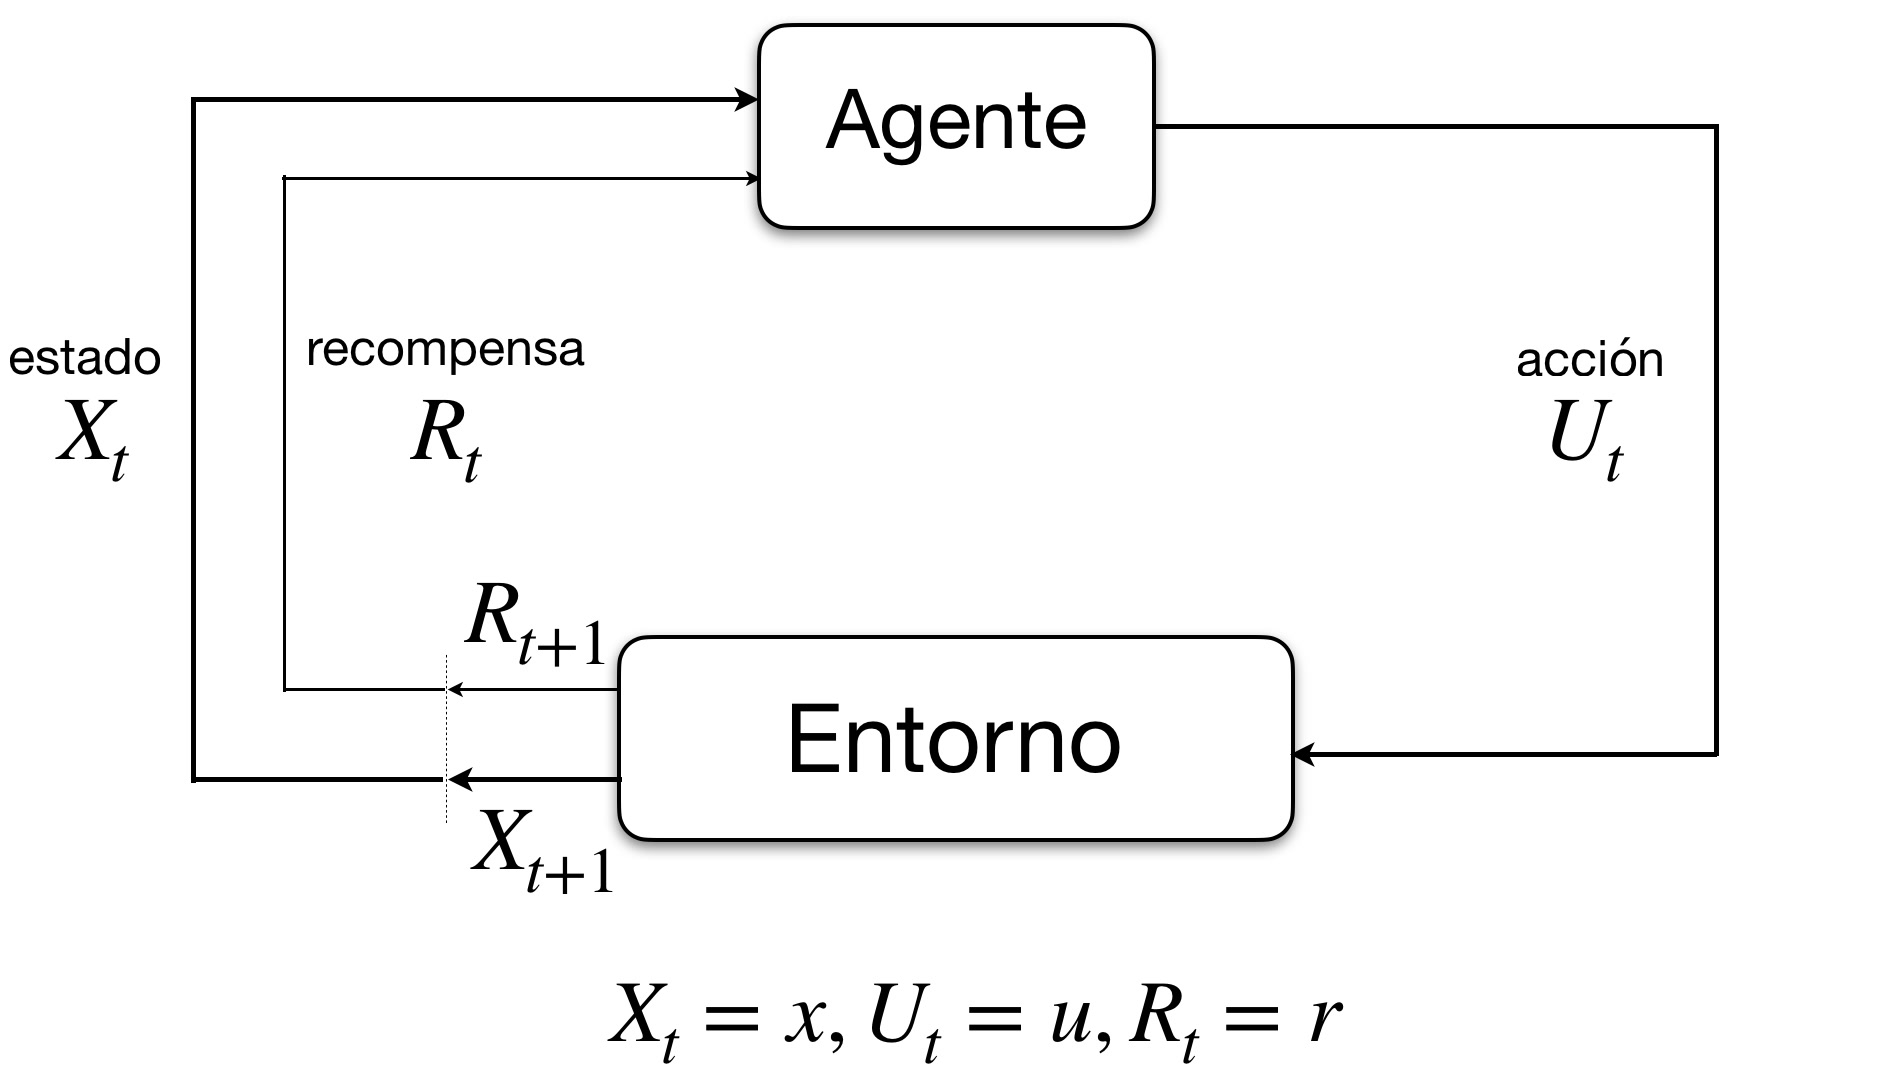
\includegraphics[width=9cm]{03_aprendizaje_por_refuerzo/framework-RL.jpeg}
\caption{Diagrama de interacción agente-entorno retomado de \cite{Sutton2018}}
\label{fig:interaccion_RL}
\end{figure}

En este paradigma de aprendizaje el objetivo del agente esta expresado formalmente en términos de la recompensa. No obstante, el objetivo del agente no es aprender a obtener la máxima recompensa en cada paso de tiempo, sino que debe encontrar la estrategia a lo largo del tiempo que permita obtener la mayor cantidad acumulada de recompensas. La idea anterior se pude expresar de la siguiente manera: la recompensa debe ser una forma de comunicar al agente el objetivo global, que es lo que se quiere conseguir y no como cumplir este objetivo diciendo que tareas secundarias deben realizarse. \cite{Sutton2018}


\subsection{Proceso de decisión de Markov}\label{MPD}
Un proceso de decisión de Markov o por su nombre en inglés \acrfull{mdp} es un modelo matemático que representa la toma de secuencial de decisiones por parte de un agente. En este modelo, se considera que un estado futuro  $x_{t+1} \in \mathcal{X}$ depende de forma probabilista de la información anterior, matemáticamente esto se expresa como,
$$x_{t+1} \sim \mathbb{P}[x_{t+1} |u_t].$$
En otras palabras, la probabilidad de obtener precisamente $x_{t+1}$ esta condicionada a la historia del agente, es decir, donde estuvo y que decisiones tomó. Sin embargo, modelar que los estados futuros $x_{t+1}$ dependan de todos los estados y acciones anteriores resulta una tarea bastante compleja y poco práctica. Una simplificación de este planteamiento consiste en establecer que los estados $x_{t+1}$ sólo dependen de la información del paso anterior: $x_t$ y $u_t$. Bajo este supuesto, las probabilidades de transición tienen la propiedad de Markov, lo que transforma a dicha probabilidad en la siguiente expresión \cite{Sutton2018}, 
$$x_{t+1} \sim \mathbb{P}[x_{s+1} |x_t, u_t].$$

Esta simplicidad de plantear a los problemas de aprendizaje, no reduce la utilidad de esta formulación, pues muchos problemas pueden ser planteados como este tipo de procesos, por ejemplo: juegos, sistemas control robótico, estrategias de planeación, entre otros \cite{laura2020}.

A continuación se presenta una descripción formal 

\begin{definition}\label{def:MDP} Sea $\mathcal{M} =\{\mathcal{X}, \mathcal{U}, \mathcal{P}, \gamma, \mathcal{R}\}$  un \textbf{proceso de decisión de Markov} finito, donde,
\begin{itemize}
    \item $\mathcal{X}$ representa un conjunto finito de estados.
    \item $\mathcal{U}$ representa un conjunto finito de acciones.
    \item $\mathcal{P}$ representa el conjunto de probabilidades de transición de estado. Para $u \in \mathcal{U}$ , $x$ y $x' \in \mathcal{X}$ existe 
    $p(x'|x, u) \in \mathcal{P}$ tal que,
    $$p(x'|x,u) = \mathbb{P}\left[X_{t+1}=x'|X_t=x, U_t =u\right].$$
    \item $\gamma \in [0,1]$ representa el factor de descuento.
    \item $\mathcal{R}$ representa el conjunto de recompensas que están en función de los elementos de los espacios de estados y acciones. Es decir, para $x \in \mathcal{X}$ y $u\in \mathcal{U}$ la recompensa $r(x, u) \in \mathcal{R}$ esta dada por la siguiente expresión,
    $$r(x, u)= \mathbb{E}[R_{t+1}|X_t=x, U_t=u].$$
\end{itemize}
\end{definition}
El modelo planteado por la definición \ref{def:MDP}  guarda una estrecha relación con la teoría de control óptimo. Un problema de control óptimo con un espacio discreto de estados y acciones y transiciones de estados probabilistas es un proceso de decisión de Markov \cite{Todorov2006}.

La dinámica de un \acrshort{mdp} se desarrolla de la siguiente forma: se empieza en un estado inicial $x_0 \in \mathcal{X}$ y de acuerdo a este estado se elije $u_0 \in \mathcal{U}(x_0)$, de forma estocástica esta decisión termina en un estado $x_1 \in \mathcal{X}$, este evento lo caracteriza $p(x_1|x_0, u_0)$. Estando en $x_1$, se toma $u_1$ y con la probabilidad $p(x_2|x_1, u_1)$ se llega al estado $x_2$ \cite{Han2018AMI}. Este sucesión de estados y acciones continua iterativamente y se representa de la siguiente forma, 
$$x_0 \xrightarrow{u_0} x_1 \xrightarrow{u_1} x_2 \xrightarrow{u_2} \cdots x_{t-1} \xrightarrow{u_{t-1}} x_{t} \xrightarrow{u_t} \cdots.$$

En el aprendizaje por refuerzo, el agente no necesariamente tiene conocimiento las probabilidades de transición. Basta con que tenga una noción de dichas transiciones por medio de los estados, acciones y recompensas, que obtiene de la interacción con el agente. 

\subsection{Episodios y retornos} 

Hasta ahora no se ha definido una estructura temporal sobre la interacción entre el agente y el entorno. Para ello es necesario entender que la transición de un estado a otro ocurre en paso de tiempo discreto. Es decir, cuando el agente esta en un estado $x$ al tiempo $t$, elije una acción $u'$ , eso lo lleva a estar $x'$ y recibir una recompensa $r$ en el paso de tiempo $t +1$. Esta sucesión de transiciones definirá la evolución de la historia que el agente ha recorrido. Formalmente esta sucesión de transiciones se define como trayectoria y episodio en el caso que exista un estado terminal. 

\begin{definition} Para un índice de tiempo arbitrario $t >0$, sea $\tau$ una sucesión de eventos en términos de los estados, acciones y recompensas. Esta sucesión se define como, 
$$\bm\tau = \{x_0, u_0, r_1, x_1, u_1, \cdots, x_{t-1}, u_{t-1}, r_{t-1}, x_t\}.$$
A esta expresión se le conoce como \textbf{trayectoria} y representa la información pasada a la que el agente ya tuvo acceso previamente.

Sea $T >0$. Una trayectoria $\mathbf{E}$, cuyo último estado es terminal, es decir, un estado para el cuál ya se logro el objetivo de realizar la tarea o se acabo el tiempo, se le conoce como \textbf{episodio},
$$\mathbf{E} = \{x_0, u_0, r_1, x_1, u_1, \cdots, x_{T-1}, u_{T-1}, r_{T}, x_{T}\}.$$
Un episodio es un caso particular de las trayectorias pues representa el historial de eventos que recorre un agente de principio a fin. 
\end{definition}

Ahora que se tiene una definición de episodio, resulta de gran interés definir el objetivo global del agente en términos de la evolución del sistema. Para ello se introduce el concepto de retorno.

\begin{definition}
 Sea $t>0$ el paso de tiempo actual y sea $T>0$ el paso de tiempo final. Se define a $G_t$ como el \textbf{retorno} al paso de tiempo $t$ y esta dada por la siguiente expresión, 
 $$G_t = R_{t+1} + R_{t+2} + \cdots + R_{T}.$$
 \end{definition}
 
 En la definición anterior se observa que el retorno esta dado por la suma acumulada de recompensas de los tiempos futuros. A pesar de que la expresión $G_t$ ayuda a definir el objetivo del agente, resulta una definición incompleta. Ya que para el caso de tareas continuas $(T\rightarrow\infty)$ no es posible trabajar numéricamente con sumas infinitas. Para ello es necesario ampliar la definición para obtener con retornos finitos.

\begin{definition}
 Sea $\gamma$ la \textbf{tasa de descuento} aplicado al retorno. El retorno $G_t$ con descuento esta definido por la siguiente expresión, 
 $$ G_{t} = R_{t+1} + \gamma R_{t+2} + \gamma^2 R_{t+3} + \cdots = \sum_{k=0}^{\infty} \gamma^{k} R_{t+k+1}.$$
\end{definition}

\begin{remark}\label{obs:return}
    Las observaciones de pasos sucesivos están relacionados entre si. 
    \begin{align*}
        G_t &= R_{t+1} + \gamma R_{t+1} + \gamma^2 R_{t+2} + \gamma^3 R_{t+3} + \cdots \\
        &= R_{t+1} + \gamma G_{t+1}
    \end{align*}
\end{remark}
Esta nueva definición del retorno no sólo es numéricamente estable, si no que también tiene una propiedad adicional bastante intuitiva. Si el valor de $\gamma$ se aproxima a $0$, tendrán poco peso las recompensas adelante del tiempo $t$. Por el contrario si el valor de $\gamma$ es cercano a $1$, las recompensas a lo largo del tiempo 
aportaran un valor significativo. Esta propiedad permite hacer un balance entre la importancia que le dará el agente entre optimizar futuras recompensas o priorizar la obtención de recompensas inmediatas. Debido a las propiedades que ofrece usar la tasa de descuento $\gamma$, esta será utilizada incluso en problemas episódicos. \cite{Sutton2018}

\subsection{Política y funciones de valor}
Los conceptos de procesos de Markov y retornos esperados sientan las bases para definir el criterio de selección de acciones, llamado política. Así como 
la evaluación de dicho criterio por medio de las denominadas funciones de valor. 

La política se puede entender como la estrategia de actuación que sigue un agente dado que se encuentra en estado. La política determina por completo el comportamiento de un agente \cite{silver2015}. Formalmente,
la política se define como el mapeo de estados a probabilidades de seleccionar cada una de las diferente acciones disponibles \cite{Sutton2018}. 
\begin{definition}
    Sea $\pi: \mathcal{S} \rightarrow \mathcal{P}(\mathcal{A})$ la función de densidad de una distribución de las acciones dado el estado. 
    $$\pi(u|x) = \mathbb{P}\left[U_t=u|X_t=x\right].$$
    Esta distribución de probabilidad lleva el nombre de \textbf{política}.
\end{definition}

Los métodos de aprendizaje por refuerzo tienen como objetivo encontrar la mejor" política disponible para el agente. Esta política deberá ser la mejor estrategia para optimizar la cantidad de recompensas. En muchos casos el diseño de políticas involucra la estimación de que tan bien se esta desempeñando el agente, es decir, que tan bien funciona la política del agente para cumplir su objetivo. Esta noción de buen desempeño se define en términos de los futuros recompensas o de acuerdo a la acumulación esperada de las recompensas según la política utilizada en cierto estado  \cite{Sutton2018}. Un buen comportamiento no sólo es medido en función del estado, si no que también lo puede estar en términos de la acción elegida. Este desempeño se define a partir de las funciones de valor. 

\begin{definition}
    Sea $V_{\pi}: \mathcal{X} \rightarrow \mathbb{R}$ la \textbf{función valor de estado} (state-value function) de un proceso de decisión de Markov. Esta función se define como el retorno esperado de empezar en $x \in \mathcal{X}$ siguiendo la política $\pi$.
    $$V_{\pi}(x)= \mathbb{E}_{\pi}\left[G_t | X_t=x\right]$$. 

    Sea $Q_{\pi}: \mathcal{X}\times\mathcal{U}\rightarrow \mathbb{R}$ la \textbf{función valor de acción} (action-value function).
    Esta función se define como el valor esperado del retorno empezando por $x\in \mathcal{X}$ , eligiendo $u \in \mathcal{U}(x)$ y las próximas acciones de acuerdo a la política $\pi$. 
    $$Q_{\pi}(x, u)= \mathbb{E}_{\pi}\left[G_t | X_t=x, U_t=u\right].$$
\end{definition}

A partir de estas funciones, los algoritmos de aprendizaje por refuerzo conectan futuras recompensas con acciones actuales \cite{prince2023understanding}. En las siguientes secciones se verá que esta relación es fundamental para poder entrenar agentes capaces de resolver tareas complejas a lo largo del tiempo. 

\begin{remark}
    El valor de acción esta estrechamente relacionado con el valor de estado, como se exhibe en la siguiente expresión,
    \begin{align*}
        \underbrace{\mathbb{E}_{\pi}[G_t|X_t=x]}_{V_{\pi}(x)} &= \sum_{u\in\mathcal{U}(x)}\pi(u|x)\underbrace{\mathbb{E}_{\pi}[G_t|X_t=x, U_t=u]}_{Q_{\pi}(x,u)},
    \end{align*}
    en consecuencia, 
    $$V_{\pi}(x) = \sum_{u\in \mathcal{U}(x)}\pi(u|x)Q_{\pi}(x, u).$$
\end{remark}

\section{Principio de Optimalidad}

Ahora se mencionaran los criterios que pueden resolver el problema de aprendizaje. Resolver este problema implica encontrar una política que consiga acumular la mayor cantidad de recompensas a lo largo del tiempo \cite{Sutton2018}. Con las hipótesis establecidas hasta ahora, es posible encontrar una política que consiga dicho objetivo. La política que mejor cumpla este objetivo, será definida como política óptima.

\subsection{Ecuación de Bellman}
Ahora se presentan las ecuaciones de Bellman. Estas ecuaciones permitirán estudiar condiciones de optimalidad para las funciones de valor y políticas. En consecuencia, esto permitirá desarrollar un métodos capaces de resolver el problema de aprendizaje.

 Las funciones de valor tienen una propiedad fundamental que es ampliamente usada dentro del aprendizaje por refuerzo \cite{Sutton2018}. Esta propiedad consiste en que las funciones de valor satisfacen una relación recursiva, como se muestra a continuación, 
\begin{align}
    V_{\pi}(x) &= \mathbb{E}_{\pi}[R_{t+1}|X_t=x] + \gamma\mathbb{E}_{\pi}[G_{t+1}|X_t=x] \\
    &= \sum_{u}\pi(u|x) \mathbb{E}_{\pi}[R_{t+1}|X_t=x, U_t=u] + \gamma \sum_{u}\pi(u|x)\sum_{x'}p(x'|x, u)V_{\pi}(x') \\
    &= \sum_{u}\pi(u|x)\left[r(x,u) + \gamma \sum_{x'}p(x'|x,u)V_{\pi}(x')\right].
    \label{eq:Bellman_V}
\end{align}

La expresión \ref{eq:Bellman_V} lleva por nombre \textbf{ecuación de Bellman} para $V_{\pi}$. Esta ecuación expresa la relación que hay entre el valor de un estado y los valores de los estados subsecuentes. Adicionalmente, esta ecuación es un mapeo de contracción y por lo tanto tiene solución única. Esto será relevante para generar algoritmos computacionales de aprendizaje \cite{Shiyu2022}.

También es posible escribir la ecuación de Bellman en términos del valor acción, como se muestra debajo,
\begin{align*}
    Q_{\pi}(x, u) &= r(x,u) + \gamma \sum_{x'}p(x'|x,u)V_{\pi}(x') \\
    &= r(x,u) + \gamma \sum_{x'}p(x'|x,u)\sum_{u'}\pi(u'|x')Q_{\pi}(x', u').
\end{align*}
La segunda igualdad es resultado de la observación \ref{obs:return}.

Estas ecuaciones no sólo permite expresar al cálculo de funciones de valor como un problema de punto fijo, también permiten encontrar mejores políticas para resolver el problema de aprendizaje como se estudiará más adelante.

\subsection{Política óptima y funciones óptimas de valor}

Para definir una política óptima es necesario establecer un orden parcial sobre las políticas. Una política $\pi_1$ se dice que es mejor que o igual que otra política $\pi_2$, si su retorno esperado es mayor o igual al de $\pi_2$ para todos los estados. Matemáticamente, esto se puede expresar de la siguiente manera,
$$ \pi_1 \geq \pi_2 \quad \iff \quad V_{\pi_1}(x) \geq V_{\pi_2}(x) \quad \forall x \in \mathcal{X}.$$
Bajo este principio, al menos se tiene acceso a una política que es mejor o igual que otras políticas. Dicha política se le denomina \textbf{política óptima} y se le denota por $\pi_{*}$. \cite{Sutton2018}

En general no hay garantía de que la política $\pi_{*}$ sea única. No obstante, por el principio de orden parcial sobre las políticas, se puede afirmar que las políticas óptimas comparten las mismas funciones de valor. En concreto la \textbf{función óptima valor estado} esta dada por la siguiente expresión,
$$V_{*}(x) = \max_{\pi}V_{\pi}(x) \quad \forall x \in \mathcal{X}.$$
Por otro lado, la \textbf{función óptima de valor acción} esta definida de la siguiente forma \cite{Sutton2018},
\begin{align}
Q_{*}(x, u) = \max_{\pi}Q_{\pi}(x,u) \quad \forall x \in \mathcal{X}, \quad \forall u \in \mathcal{U}.
\label{eq:optimal_Q}
\end{align}

Hasta ahora no se ha caracterizado a la política óptima. Como se mencionó anteriormente, no existe una única política óptima. Sin embargo, siempre se puede diseñar una política óptima en términos de la expresión \ref{eq:optimal_Q}, como se muestra a continuación \cite{Sutton2018}, 
\begin{align}
    \pi_{*}(u|s) = 
    \begin{cases}
    1 & \text{Si } u= \argmax_{u} Q_{*}(x, u) \\
    0 & \text{e.o.c}
    \end{cases}.
\label{eq:greedy_policy}
\end{align}

A la política óptima dada por la expresión \ref{eq:greedy_policy} se le llama \textbf{política voraz} o \textit{\textbf{greedy policy}}. Esta política se puede escribir como una densidad de probabilidad o como la ley de control,
\begin{align*}
    \mu_{*}(x) = \argmax_{u}Q_{*}(x, u) \quad \forall x \in \mathcal{X}.
\end{align*}

Merece especial atención que se puede expresar a la función $V_{*}$ sin hacer referencia explicita a alguna política óptima. Basta con observar la relación que guarda las función óptima de $V$ debe ser igual la función $Q$ de la política óptima, dado que se toma la mejor acción disponible. Lo anterior se traduce en la siguiente expresión \cite{Sutton2018},
\begin{align}
    V_{*}(x) &= \max_{u \in \mathcal{U}(x)} Q_{\pi_{*}}(x, u) \\
    &= \max_{u}\left[r(x,u) + \gamma \sum_{x'}p(x'|x,u)V_{*}(x')\right]. 
    \label{eq:optimal_V}
\end{align}


\section{Aprendizaje en sistemas de control}

El marco teórico, así como las políticas y funciones óptimas de valor necesitan contextualizarse en un planteamiento concreto para resolver problemas reales. Por ejemplo en los planteados por los sistemas de control. Como se discutió anteriormente, los sistemas de control se formulan a partir de espacios de acciones y estados continuos. Para resolver problemas de esta naturaleza, será necesario definir el proceso de decisión de Markov para espacios continuos. 

Este nuevo planteamiento supone un reto para el cálculo de políticas óptimas y funciones de valor. Esto implica un cambio en la representación de las políticas y las funciones de valor. Debido a la naturaleza de los espacios de estados y acciones continuas, no es tarea sencilla definir dichas instancias. Existen varios algoritmos que tienen el objetivo de encontrar un solución aproximada al óptimo teórico. Estos algoritmos deben ser computacionalmente eficientes tales que puedan ser usados en tiempo real y posean eficiencia de muestreo de tal forma que puedan aprender usando poca información \cite{wiering2011}. Los algoritmos usados en este trabajo incorporan elementos del aprendizaje profundo \ref{sec:DL} para estimar funciones de valor y obtener políticas óptimas. Otra disyuntiva patente en este contexto, es el conocimiento o no de un modelo que conforme la estructura del entorno. Esta encrucijada motiva a plantear dos enfoques del aprendizaje por refuerzo. El primer enfoque se basa en usar la información disponible del modelo con el fin de planear estrategias para el agente. En cambio, el segundo se apoya en el aprendizaje por medio de prueba y error para diseñar estrategias para el agente.

\subsection{Procesos de decisión de Markov en espacios continuos}

Ahora se establecerán las características e hipótesis que se seguirán para resolver el problema de control de vuelo de un cudricoptero. Para empezar, se introducirá el concepto de \acrshort{mdp} en espacios continuos. Posteriormente, se examinará la forma de representar a las políticas y funciones de valor como redes neuronales. Finalmente, se discutirán los conceptos de planeación y aprendizaje.

Retomando la formulación establecida en la sección \ref{sec:marco_teorico}, un proceso de decisión de Markov $\mathcal{M}$ se conforma de la tupla $\left\{\mathcal{X}, \mathcal{U}, \mathcal{P}, \mathcal{\gamma}, \mathcal{R}\right\}$. En este contexto el espacio de estados $\mathcal{X}$ generalmente es un conjunto no numerable y acotado \cite{wiering2011}. Para tareas de control se puede asumir que el conjunto de estados es un subconjunto de un espacio euclidiano multidimensional, tal que $\mathcal{X}\subset\mathbb{R}^{n_x}$, dónde $n_x \in \mathbb{N}$ representa la dimensión de cada estado. De la misma forma para un espacio de acciones continuas se asume que $\mathcal{U}\subset \mathbb{R}^{n_u}$, dónde $n_u$ representa la dimensión del espacio de acciones. Bajo esta formulación es necesario establecer una notación vectorial para los estados y acciones, tal que $\mathbf{x}\in \mathcal{X}$ y $\mathbf{u}\in \mathcal{U}$ representan las variables de estado y acción, correspondientemente. Esta notación coincide con la usada para los sistemas de control. Bajo este nuevo tratamiento los estados y acciones se describen como variables aleatorias continuas. Esta nueva caracterización implica un cambio en la descripción de expresiones fundamentales como las ecuaciones de Bellman. Por ejemplo, la función de valor acción se expresa de la siguiente manera,
\begin{align}
    Q_{\pi}(\mathbf{x}, \mathbf{u}) = r(\mathbf{x}, \mathbf{u})+ \gamma \int_{\mathcal{X}}p(\mathbf{x}'|\mathbf{x}, \mathbf{u})V_{*}(\mathbf{x}')d\mathbf{x}
   \label{eq:bellman_Q2_cont}.
\end{align}

Para los sistemas de control la probabilidad de transición $p(\mathbf{x}'|\mathbf{x}, \mathbf{u})$ en \ref{eq:bellman_Q2_cont} representa la evolución del sistema dinámico en cada paso de tiempo. En general esta expresión se modela desde una perspectiva estocástica. No obstante, esta definición es compatible con los sistemas dinámicos deterministas, si se establece la siguiente relación,
$$p(\mathbf{x}'|\mathbf{x}, \mathbf{u}) = \mathds{1}_{\mathbf{x}'=f(\mathbf{x}, \mathbf{u})},$$
dónde $f$ representa el sistema dinámico.

Otra aclaración importante es que al igual que la función de costo en control óptimo, la función recompensa $r$ se considerara como una función determinista, como se expresa a continuación, 
\begin{align}
    r : \mathcal{X}\times\mathcal{U}&\rightarrow \mathbb{R} \\
    (\mathbf{x}, \mathbf{u})&\rightarrow r(\mathbf{x}, \mathbf{u})
    \label{eq:reward_function}.
\end{align}
Esta simplificación resulta útil para determinar la forma de la recompensa. Además permite ligar las capacidades de control óptimo con el aprendizaje por refuerzo.

\subsection{Configuraciones de aprendizaje en espacios continuos}

El principal objetivo de un problema de control es encontrar un política óptima. Sin embargo, en un \acrshort{mdp} con espacios continuos, no es posible encontrar directamente una para esto se requieren condiciones más fuertes sobre los espacios de estados y acciones \cite{Sutton2018}. En lugar de ello se desea encontrar una aproximación de dicha política. 

Como se discutió anteriormente, la política óptima depende de la función de valor óptima, que a su vez esta subordinada a  un \acrshort{mdp}. A partir de este hecho se consideran tres enfoques generales para resolver el problema de aprendizaje. El primer enfoque lleva por nombre \textbf{métodos basados en modelos} (\textit{\textbf{model-based methods}}). Este tipo de algoritmos se basan en un el uso de un modelo (aprendido o conocido) con el fin de aproximar una función de valor o política global \cite{Moerland2018}. Este enfoque se basa en la combinación de técnicas de planificación y aprendizaje. Este tipo de algoritmos combinan los mecanismos descritos por la línea punteado y la línea continua en la figura \ref{fig:RL_configuration}. 

El segundo enfoque es conocido como \textbf{métodos basados en valores} (\textit{\textbf{value-based methods}}). Esta clase de algoritmos tienen la finalidad de construir una representación de la función de valor, que posteriormente permite definir una política \cite{franccois2018}. 

El último conjunto de algoritmos lleva por nombre \textbf{métodos basados en políticas} (\textit{\textbf{policy-based methods}}). Los algoritmos basados en valores infieren una política indirectamente, al estimar los valores de las acciones y estados. En cambio, los métodos basados en políticas almacenan una representación de la política. El proceso de aprendizaje implica actualiza sucesivamente dicha representación. El objetivo de este proceso es aproximar una política óptima.

Estas diferentes clases de algoritmos no se excluyen mutuamente. Usualmente, los métodos basados en políticas y valores conforman un enfoque más amplio denominado \textbf{aprendizaje por refuerzo sin modelos} (\textbf{\textit{model-free} \acrshort{rl}}). Este enfoque se centra
en optimizar políticas y funciones de valor por medio de las experiencias obtenidas a lo largo de la interacción del agente y el entorno. Como su nombre lo menciona, el aprendizaje en este enfoque no se basa en el uso de un modelo de la dinámica. En cambio, el diseño de las políticas óptimas por medio de una estrategia de prueba y error. Los algoritmos sin modelos se caracterizan por seguir únicamente el proceso descrito por la línea continua de la figura \ref{fig:RL_configuration}.

Habitualmente, se suele pensar que los métodos basados en modelos son la contra parte de aquellos sin modelos.
Pues, al utilizarse un modelo los algoritmos pueden enfocarse en anticipar el futuro. En tanto que cuando se ignora el modelo, la aproximación depende por completo de las experiencias pasadas. 

\begin{figure}[h!]
\centering
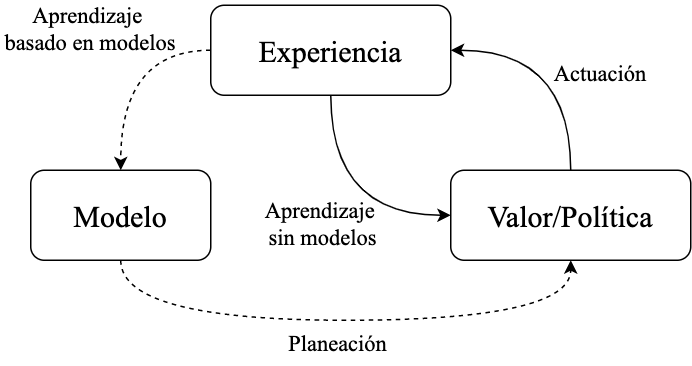
\includegraphics[width=9cm]{03_aprendizaje_por_refuerzo/rl_configuration.png}
\caption{Esquema general de diferentes métodos de \acrshort{rl} \cite{franccois2018}. El enfoque directo usa una representación de la función de valor política para actuar en el entorno. El enfoque indirecto usa un modelo del entorno.}
\label{fig:RL_configuration}
\end{figure}

Con el fin de de aproximar las funciones de valor y políticas se integra el ajuste de redes neuronales al aprendizaje por refuerzo. Entre las ventajas de usar redes neuronales en este contexto se encuentran las siguientes:
\begin{itemize}
    \item Las redes neuronales tienen la capacidad de reconocer patrones ocultos, esta cualidad es fundamental para entender la dinámica de un sistema con el fin de tomar una decisión informada \cite{baeldung2023RL}. 
    \item Las redes neuronales pueden ser ajustadas usando actualizaciones incrementales, esto le permite aprender en cada interacción con el entorno \cite{gosaviaRL}. 
    \item Las redes neuronales tienen la capacidad de aproximar funciones con alta precisión y generalizar de manera efectiva a partir de unos pocas muestras de entrenamiento \cite{wiering2011}. 
\end{itemize}

En los siguientes capítulos la discusión se centrará en el estudio de métodos basados en modelos y sin modelos, con el fin de obtener una metodología viable para el objetivo de este trabajo. En el capítulo \ref{chapter:model_based} se estudiará un algoritmo que tiene la finalidad de aproximar una política óptima a partir de una estrategia informada por el modelo. Para el enfoque sin modelos en el capítulo \ref{chapter:model_free} se estudiarán métodos para aproximar la función óptima de Bellman y diseñar una política óptima, por medio del uso de redes neuronales.



\chapter{Búsqueda guiada de políticas (GPS)}
\label{chapter:model_based}

Los métodos de \textbf{búsqueda guiada de políticas} o por su nombre en inglés \textbf{\acrfull{gps}} se han convertido en una herramienta importante en el área de aprendizaje por refuerzo. Estos métodos son una clase de algoritmos de búsqueda de política \footnote{Los \textbf{métodos de búsqueda de política} conforman un subcampo de \acrshort{rl} que se enfoca en encontrar la configuración adecuada de una política parametrizada dada. Estos métodos pueden ser utilizados para aprender políticas a partir de muestras de trayectorias, convirtiéndolos en un enfoque general del aprendizaje de robots. \cite{PetersNeumann2015}} que utilizan métodos de optimización de trayectorias para generar datos de entrenamiento \cite{Du_2021}. Estos datos de entrenamiento son trayectorias utilizadas para guiar el aprendizaje de políticas parametrizadas, como redes neuronales artificiales. Los métodos \acrshort{gps} combinan la teoría de optimización convexa y aprendizaje profundo, esto ha permitido conseguir magníficos resultados en complejas tareas de control como el aprendizaje de robots. 
% Policy search methods are a subfield of reinforcement learning that focus on finding good parameters for a given policy parametrization

En este capítulo se hará un descripción detallada del método, la cual esta ampliamente basada en lo expuesto en \cite{Schneider2018} y \cite{Deep_Visuomotor_Policies}.

\section{Definición del problema}

En la búsqueda de políticas el objetivo es aprender una política $\pi_{\bm\theta}(\mathbf{u}_t| \mathbf{x}_t)$ que permita a un agente elegir acciones $\mathbf{u}_t$ en respuesta a estados $\mathbf{x}_t$ para controlar un sistema dinámico, como un cuadricóptero \cite{Deep_Visuomotor_Policies}. En este caso $\bm{\theta}$ denota los parámetros de la política que deben ser optimizados para la tarea, que en este caso representa a los pesos de una red neuronal artificial o mejor conocida como \acrfull{ann}. Una descripción más detallada de este tipo de modelos se encuentra en el apéndice \ref{sec:DL}. 

Con el fin de obtener una política, el algoritmo \acrshort{gps} plantea el siguiente problema de optimización, 
 \begin{align}
    \min_{p, \bm\theta} \sum_{i=1}^{N}\mathbb{E}_{\bm\tau \sim p_{i}}\left[c(\bm\tau)\right] \quad \text{sujeto a} \quad p_{i}(\mathbf{u}_t|\mathbf{x}_t) = \pi_{\bm\theta}(\mathbf{u}_t|\mathbf{x}_t),
    \label{eq:gps_objective}
\end{align}
dónde $c(\bm\tau)$ representa el costo acumulado a lo largo de una trayectoria $\bm\tau$, que se conforma por una secuencia temporal de parejas $(\mathbf{x}_t, \mathbf{u}_t)$. Este costo acumulado también se puede representar de la siguiente manera, 
\begin{align}
    c(\bm\tau) = \sum_{t=1}^{T}c(\mathbf{x}_t, \mathbf{u}_t)
    \label{eq:traj_cost}.
\end{align}
Cada trayectoria $\bm\tau$ esta dada por una distribución de probabilidad como se muestra en la siguiente igualdad,
\begin{align}
    p_{i}(\bm\tau) = p_{i}(\mathbf{x}_1)\prod_{t=1}^{T-1}p(\mathbf{x}_{t+1}|\mathbf{u}_t, \mathbf{x}_t)p_{i}(\mathbf{u}_t|\mathbf{x}_t),
    \label{eq:tray_dist}
\end{align}
dónde $p(\mathbf{x}_{t+1}|\mathbf{u}_t, \mathbf{x}_t)$ se refiere a la distribución del sistema dinámico discutida en la sección \ref{MPD}. Mientras que $p_i(\mathbf{x}_1)$ es la distribución inicial de estados y  $p_i(\mathbf{u}_t|\mathbf{x}_t)$ representa el $i$-esímo controlador local variable en el tiempo. 

\section{Optimización}
La expresión \ref{eq:gps_objective} es un problema dual, que se ha resuelto optimizando el langrangiano asociado a dicha expresión por medio del método descenso de gradiente dual  (\textit{dual gradient descent}). Este método consiste en alternar la optimización del lagrangiano con respecto a las variables primarias $p_i(\bm\tau)$ y $\bm\theta$ y la actualización de los multiplicadores de Lagrange usando el gradiente del lagrangiano evaluado en las nuevas variables primarias. \cite{2014-mfcgps} 

El algoritmo \acrshort{gps} divide la resolución del problema \ref{eq:gps_objective} en un paso para cada variable primaria. El primero paso se refiere a la obtención de los distintos $N$ controladores locales $p_i$. Esto se logra por medio de la minimización del valor esperado del costo $c$ de las trayectorias $\{\bm\tau_i\}_{i}$ resultantes de cada estado inicial. A este paso se le denota como \textbf{optimización de trayectorias locales}. Es importante notar que cada controlador es entrenado únicamente en un estado inicial específico y que es probable que no tenga éxito en estados fuera de la distribución. En la práctica estos controladores no son suficientes para resolver una tarea en general. Sin embargo, se utilizan para generar datos de entrenamiento para un algoritmo de aprendizaje supervisado (para más detalles consultar \ref{sec:supervised_learning}), que conforma el segundo componte de \acrshort{gps}. Este componente consiste en entrenar una política global independiente del tiempo $\pi_{\mathbf{\bm\theta}}$, que se asemeje al comportamiento de todos los $N$ controladores locales. A este componente del algoritmo se le conoce como  \textbf{optimización de la política global}.  \cite{Schneider2018}

Al igual que lo realizado en \cite{Deep_Visuomotor_Policies}\cite{Schneider2018}, este trabajo utilizará una versión modificada del método del descenso de gradiente dual conocido como  \acrfull{badmm} \cite{wang2014bregman} para optimizar los controladores locales y la política global.

\subsection{\acrshort{badmm}}
El método de \acrshort{badmm} es utilizado para resolver problemas duales de la siguiente forma,
\begin{align}
    \min_{\mathbf{v} \in \mathcal{V}, \mathbf{z} \in \mathcal{Z}} f(\mathbf{v})+ g(\mathbf{z}) \quad \text{sujeto a} \quad \mathbf{A} \mathbf{v} + \mathbf{B} \mathbf{z} = \mathbf{c}.
    \label{badmm_problem}
\end{align}
Por hipótesis se establece que $f$ y $g$ son funciones convexas, $\mathbf{A}\in \mathbb{R}^{m \times n_{v}}$, $\mathbf{B} \in \mathbb{R}^{m \times n_{z}}$, $\mathbf{c}\in \mathbb{R}^{m \times} 1$. En este caso $\mathbf{v}\in \mathcal{V}\subset\mathbb{R}^{n_v \times 1}$ y $\mathbf{z} \in \mathcal{Z}\subset\mathbb{R}^{n_z \times 1}$ representan las variables primarias, dónde $\mathcal{V}$, $\mathcal{Z}$ son conjuntos convexos. El lagrangiano asociado al problema \ref{badmm_problem} es el siguiente,
\begin{align}
    \mathcal{L}(\mathbf{v}, \mathbf{z}, \lambda) = 
    f(\mathbf{v}) + g(\mathbf{z}) + \langle\bm\lambda, \mathbf{A v} + \mathbf{B z} -\mathbf{c}\rangle + \nu B_{\chi}(\mathbf{c} - \mathbf{Av}, \mathbf{B z}), 
    \label{BADMM_lagrangian}
\end{align}
dónde los términos $\bm\lambda \in \mathbb{R}^{m}$ y $\nu \in \mathbb{R}$ que representan el multiplicador de Lagrange y un factor de penalización, respectivamente. \cite{wang2014bregman}

En lugar de utilizar una distancia euclidiana, como otros métodos que emplean regularización, este método utiliza la divergencia de Bregman, cuya notación es $B_{\chi}$. El uso de esta divergencia permite explotar la estructura del problema y ofrece una convergencia más rápida que otros métodos como \acrfull{admm}. \cite{wang2014bregman} 

\begin{definition}
    Sea $\chi: \Omega \rightarrow \mathbb{R}$ una función continuamente diferenciable y estrictamente convexa y definida en el conjunto convexo $\Omega$. La divergencia de Bregman asociada a $\chi$ de los elementos $p, q \in \Omega$ esta dado por la siguiente expresión,
    $$B_{\chi}(p, q) := \chi(p)-\chi(q)-\left(\nabla \chi(q), p-q\right).$$
\end{definition}
Este método establece las siguientes reglas de actualización para las variables primarias y el multiplicador de Lagrange, 
\begin{align*}
    \mathbf{v}^{(k+1)} &= \argmin_{\mathbf{v}\in \mathcal{V}} \left(f(\mathbf{v}) + \left\langle \bm\lambda^{(k)}, \mathbf{Av}+\mathbf{B}\mathbf{z}^{(k)}-\mathbf{c}\right\rangle + \nu B_{\chi}\left(\mathbf{c}-\mathbf{Av}, \mathbf{B}\mathbf{z}^{(k)}\right)\right), \\
    \mathbf{z}^{(k+1)} &= \argmin_{\mathbf{z} \in \mathcal{Z}} \left(g(\mathbf{z}) + \left\langle\bm\lambda^{(k)}, \mathbf{A}\mathbf{v}^{(k+1)} + \mathbf{Bz-c}\right\rangle + \nu B_{\chi} \left(\mathbf{Bz}, \mathbf{c}-\mathbf{Av}^{(k+1)}\right)\right), \\
    \bm\lambda^{(k+1)} &= \bm\lambda^{(k)} + \alpha_{\bm\lambda}\cdot\nu \left(\mathbf{Av}^{(k+1)}  + \mathbf{Bz}^{(k+1)}-\mathbf{c}\right), 
    \label{BADMM_update}
\end{align*}
dónde $\alpha_{\bm\lambda} \in \mathbb{R}$ representa la tasa de actualización del multiplicador de Lagrange. \cite{wang2014bregman}

\subsection{\acrshort{badmm} para \acrshort{gps}}


Para utilizar el método \acrshort{badmm} en la resolución del problema \ref{eq:gps_objective} es necesario modificar la restricción entre la política y los controles locales de la siguiente manera,
$$  p_i(\mathbf{u}_t|\mathbf{x}_t)p_i(\mathbf{x}_t)= \pi_{\bm\theta}(\mathbf{u}_t|\mathbf{x}_t)p_i(\mathbf{x}_t) \quad 
    \forall i \in \mathcal{I}, t \in \mathcal{T}, \mathbf{u}_t\in \mathbb{R}^{n_u}, \mathbf{x}_t \in \mathbb{R}^{n_x} 
$$
Ahora será necesario definir los espacios $\mathcal{V}$ y $\mathcal{Z}$. En primer lugar, el conjunto $\mathcal{V}$ representa el espacio de las posibles funciones de densidad conjunta de estados y acciones asociada a la política $\pi(\mathbf{u}|\mathbf{x})$. Por otra parte, el conjunto $\mathcal{Z}$ esta dado por el espacio de las funciones de densidad de los posibles controles locales. Estos conjuntos se expresan de la siguiente manera \cite{Schneider2018},
\begin{align*}
     \mathcal{V}&=\Bigg\{ f:\mathcal{I}\times\mathcal{T}\times\mathbb{R}^{n_x}\times\mathbb{R}^{n_u}\rightarrow\mathbb{R}\Big| \left( \forall i \in \mathcal{I},\forall t \in \mathcal{T}, \forall \mathbf{u}_t\in \mathbb{R}^{n_u}, \forall\mathbf{x}_t\in \mathbb{R}^{n_x}:f_i(\mathbf{x}_t, \mathbf{u}_t)\geq 0 \right)   \\ 
    \cap & \left(\int f_i(\mathbf{x}_t, \mathbf{u}_t)d\mathbf{u}d\mathbf{x} =1\right)\Bigg\}.
\end{align*}

Para poder interpretar el problema de búsqueda de políticas \ref{eq:gps_objective} de la forma \ref{badmm_problem} es necesario 
cambiar los operadores lineales asociados a las matrices $\mathbf{A}$ y $\mathbf{B}$ por funciones lineales en una dimensión \cite{Schneider2018}. Estos cambios se expresan de la siguiente forma, 
\begin{align*}
\mathbf{A}\mathbf{v} \rightarrow a(\mathbf{v}):= -\mathbf{v}, \qquad
\mathbf{B}\mathbf{z} \rightarrow b(\mathbf{z}):= \mathbf{z}.
\end{align*}
Estas modificaciones implican que $\mathbf{c}$ debe ser 0. Adicionalmente, se requiere que las funciones $\mathbf{v}$ y $\mathbf{z}$ sean definidas como se muestra debajo,
\begin{align*}
    \mathbf{v}_i(\mathbf{x}_t, \mathbf{u}_t) := \pi_{\bm\theta}(\mathbf{u}_t|\mathbf{x}_t) p_{i}(\mathbf{x}_t), \qquad
    \mathbf{z}_i(\mathbf{x}_t, \mathbf{u}_t) := p_i(\mathbf{u}_t|\mathbf{x}_t) p_{i}(\mathbf{x}_t).
\end{align*}

Para el método \acrshort{gps} la función $f$ deberá ser idénticamente cero. Esto se debe a que la función objetivo de la expresión \ref{eq:gps_objective} sólo depende del control local, es decir, la variable $\mathbf{z}$, y no de la política $\pi_{\bm\theta}$, representada por $\mathbf{v}$. Por otro lado, la función $g$ es \cite{Schneider2018}, 
\begin{align}
    g(\mathbf{z}) &:= \sum_{i=1}^{N}\sum_{t=1}^{T} \mathbb{E}_{\mathbf{z}_{i}(\mathbf{x_t}, \mathbf{u}_t)}[c(\mathbf{x}_t, \mathbf{u}_t)] \\
    &= \sum_{i=1}^{N}\sum_{t=1}^{T}\mathbb{E}_{p_i(\mathbf{u_t}|\mathbf{x}_t)p_{i}(\mathbf{x}_t)}[c(\mathbf{x}_t, \mathbf{u}_t)]\\
    &=  \sum_{i=1}^{N}\mathbb{E}_{p_i(\bm\tau)}[c(\bm\tau)].
\end{align}

A partir de los cambios anteriores, se pueden expresar las reglas de actualización de la siguiente forma, 
\begin{align*}
    \mathbf{v}^{(k+1)} &= \argmin_{\mathbf{v}}\left( \left\langle \bm\lambda^{(k)}, \mathbf{v}-\mathbf{z}^{(k)}\right\rangle + \nu B_{\chi}\left(\mathbf{v}, \mathbf{z}^{(k)}\right)\right) \\
    \mathbf{z}^{(k+1)} &= \argmin_{\mathbf{z}}\left( \sum_{i=1}^{N}\sum_{t=1}^{T}\mathbb{E}_{\mathbf{z}_{i}(\mathbf{x}_t), \mathbf{u}_t}[c(\mathbf{x}_t, \mathbf{u}_t)] + \left\langle \lambda^{(k)}, \mathbf{v}^{(k+1)}-\mathbf{z}\right\rangle + \nu B_{\chi}\left(\mathbf{v}^{(k+1)}, \mathbf{z}\right)\right) \\
    \bm \lambda^{(k+1)} &= \bm \lambda^{(k)} + \alpha_{\bm\lambda} \cdot \nu \left(\mathbf{v}^{(k+1)}-\mathbf{z}^{(k+1)}\right).
\end{align*}

En este caso el producto escalar $\langle \cdot, \cdot \rangle: \mathcal{V}\times\mathcal{V} \rightarrow \mathbb{R}$ se define de acuerdo a la siguiente expresión,
\begin{align}
    \langle\mathbf{v}, \mathbf{z}\rangle := \sum_{i=1}^{N}\sum_{t=1}^{T}\int_{\mathcal{X}\times \mathcal{U}}\mathbf{v}_i(\mathbf{x}_t, \mathbf{u}_t) \cdot\mathbf{z}_i(\mathbf{x}_t, \mathbf{u}_t)d\mathbf{x}d\mathbf{u}. 
    \label{fun_prod}
\end{align}

Debe hacerse una observación importante sobre el multiplicador de Lagrange. En este caso es necesario que  $\lambda$ sea un elemento del espacio $\mathcal{V}$ para poder hacer uso del producto escalar. La función $\lambda:\mathcal{I}\times\mathcal{T}\times\mathcal{X}\times\mathcal{U} \rightarrow \mathbb{R}$ se define arbitrariamente en \cite{Deep_Visuomotor_Policies} como, 
$$\lambda_{i}(\mathbf{x}_t, \mathbf{u}_t) = \bm{\lambda}_{t}^{\top} \mathbf{u}_t,$$
dónde $\bm\lambda_{t} \in \mathbb{R}^{n_u}$ representa el multiplicador de Lagrange independiente del índice $i$. A pesar de que esta simplificación es bastante drástica, en la práctica esto ha hecho al método más estable \cite{Deep_Visuomotor_Policies}.

Utilizando la definición \ref{fun_prod}, se observa que el producto escalar en la regla de actualización se puede expresar de la siguiente manera,
\begin{align*}
    \left\langle\bm\lambda^{\top}_t\mathbf{u}_t, \mathbf{v}-\mathbf{z}\right\rangle &= \sum_{i=1}^{N}\sum_{t=1}^{T}\int_{\mathcal{X}\times\mathcal{U}}\bm\lambda_{t}^{\top}\mathbf{u}_t \left(\mathbf{v}_{i}(\mathbf{x}_t, \mathbf{u}_t)-\mathbf{z}_{i}(\mathbf{x}_t, \mathbf{u}_t)\right)d\mathbf{x}d\mathbf{u} \\
    &= \sum_{i=1}^{N}\sum_{t=1}^{T}\mathbb{E}_{\mathbf{v}_i(\mathbf{x}_t, \mathbf{u}_t)}\left[\bm\lambda_{t}^{\top}\mathbf{u}_t\right] - \mathbb{E}_{\mathbf{z}_i(\mathbf{x}_t, \mathbf{u}_t)}\left[\bm\lambda_{t}^{\top}\mathbf{u}_t\right].
\end{align*}
Ahora es necesario definir la divergencia de Bregman $B_{\chi}$. Ya que se esta trabajando con 
distribuciones de probabilidad de trayectorias, resulta conveniente utilizar la divergencia de \acrfull{kl}. La divergencia \acrshort{kl} es una instancia de la divergencia de Bregman, donde $\chi$ esta dada por la entropía diferencial. En este caso particular $B_{\chi}$ se representa como, 
\begin{align*}
    B_{\chi}(\mathbf{v}, \mathbf{z}) &:=\sum_{i=1}^{N}\sum_{t=1}^{T} \phi_{t}^{\bm\theta}\left(\bm\theta, p_{i}\right), \\
    B_{\chi}(\mathbf{z}, \mathbf{v})  &:=  
    \sum_{i=1}^{N}\sum_{t=1}^{T} \phi_{t}^{p}\left(p_{i}, \bm\theta\right), 
\end{align*}
dónde $\phi_t^{\bm\theta}$ y $\phi_{t}^{p}$ son los valores esperados de la divergencia \acrshort{kl} al tiempo $t$ bajo la distribución local de estados. Esto se representa en las siguientes definiciones, 
\begin{align*}
    \phi_t^{\bm\theta}\left(\bm\theta, p_i\right) &:= 
    \mathbb{E}_{p_i(\mathbf{x}_t)}\left[ D_{\text{KL}}\left(\pi_{\bm\theta}(\mathbf{u}_t|\mathbf{x}_t)|| p_i(\mathbf{u}_t|\mathbf{x}_t)\right)\right], \\
    \phi_t^{p}\left(p_i, \bm\theta\right) &:= 
    \mathbb{E}_{p_i(\mathbf{x}_t)}\left[ D_{\text{KL}}\left(
    p_i(\mathbf{u}_t|\mathbf{x}_t)|| \pi_{\bm\theta}(\mathbf{u}_t|\mathbf{x}_t)\right)\right].
\end{align*}

En este caso se sustituye la penalización $\nu$ por una multiplicador dependiente del tiempo $\nu_t$. Este cambio permitirá penalizar más a la divergencia en un paso específico de la trayectoria que en otros. Esto se hace con el fin de forzar la igualdad entre los controles locales y la política global de manera particular en cada paso de tiempo. \cite{Deep_Visuomotor_Policies}

A pesar de que las consideraciones anteriores han simplificado el problema, aun queda pendiente representar el conjunto infinito de restricciones $p_i(\mathbf{u}_t|x_t)p_i(\mathbf{x}_t)=\pi_{\bm\theta}(\mathbf{u}_t|\mathbf{x}_t)p_i(\mathbf{x}_t)$ para la actualización de $\bm\lambda$ \cite{Deep_Visuomotor_Policies}. Una forma de aproximar esta restricción, se realiza al sustituirla igualdad  con una versión que este en términos de los valores esperados de los rasgos \cite{peters2010}. Cuando estos rasgos están compuestos por funciones de variables aleatorias, esto puede ser visto como una restricción sobre los momentos de una distribución \cite{Deep_Visuomotor_Policies}. Concretamente la restricción propuesta en \cite{Deep_Visuomotor_Policies} es la siguiente, 
$$\mathbb{E}_{\pi_{\bm\theta}(\mathbf{u}_t|\mathbf{x}_t) p_i(\mathbf{x}_t)}[\mathbf{u}_t] = \mathbb{E}_{p_i(\mathbf{x}_t, \mathbf{u}_t)}[\mathbf{u}_t].$$

Tomando en cuenta los cambios anteriores, eliminando los términos independientes de las variable de actualización y sustituyendo las funciones $\mathbf{v}_i$ y $\mathbf{z}_i$ por los valores $\bm\theta$ y $p_i$, respectivamente, se pueden expresar las reglas de actualización de la siguiente manera, 
\begin{align}
    \bm\theta^{(k+1)} &= \argmin_{\bm\theta \in \Theta} \left(\sum_{i=1}^{N}\sum_{t=1}^{T}\mathbb{E}_{\pi_{\bm\theta}(\mathbf{u}_t|\mathbf{x}_t)p_i(\mathbf{x}_t)} \left[\bm\lambda_{t}^{\top(k)}\mathbf{u}_t\right] + \nu_t\phi_{t}^{\bm\theta}\left(\bm\theta, p_i^{(k)}\right)\right) \label{eq:GPS_theta}\\
    p^{(k+1)} &= \argmin_{p}\left(\sum_{i=1}^{N}\sum_{t=1}^{T} \mathbb{E}_{p_i(\mathbf{x}_t, \mathbf{u}_t)}\left[c(\mathbf{x}_t, \mathbf{x}_t) - \bm\lambda_t^{\top(k)}\mathbf{u}_t\right] + \nu_t \phi_t^{p}\left(p_i, \bm\theta^{(k+1)}\right)\right) 
    \label{eq:GPS_p}\\
    \bm{\lambda}_t^{(k+1)} &= \bm{\lambda}_t^{(k)} + \alpha_{\bm\lambda} \cdot \nu_t \left(\mathbb{E}_{\pi_{\bm\theta}(\mathbf{u}_t|\mathbf{x}_t) p_i(\mathbf{x}_t)}[\mathbf{u}_t] - \mathbb{E}_{p_i(\mathbf{x}_t, \mathbf{u}_t)}[\mathbf{u}_t]\right) \qquad \forall i \in \mathcal{I}, t \in \mathcal{T}. 
    \label{eq:GPS_lambda}
\end{align}

En las siguientes subsecciones se explicará detalladamente el proceso de optimización para cada variable del problema.

\section{Optimización de trayectorias locales}
En esta sección se revisará como utilizar el método \acrshort{ilqr} (discutido en la sección \ref{sub_sec:iLQR}) para optimizar las trayectorias generadas por los controles lineales locales. Cabe aclarar que la optimización de cada controlador $p_i$, será independiente del resto de los controladores. Por lo que en esta sección se limitará a explicar el proceso de optimización para un sólo control $p_i(\bm\tau)$. 

Para la optimización de uno de los controladores $p_i$ se toma uno de los $N$ sumandos de la expresión \ref{eq:GPS_p}, como se muestra a continuación, 
\begin{align}
    \mathcal{L}_{p_i}(p_i, \bm\theta) &= \sum_{t=1}^{T}\mathbb{E}_{p_i(\mathbf{x}_t, \mathbf{u}_t)}\left[c(\mathbf{x}_t, \mathbf{u}_t)-\bm{\lambda}_t^{\top}\mathbf{u}_t
    \right] + \nu_t \phi_{t}^{p}(p_i, \bm\theta)
    \label{eq:local_opt}
\end{align}
Para poder optimizar la expresión \ref{eq:local_opt} usando el método de \acrshort{ilqr}, se hace la siguiente modificación sobre el termino de la divergencia \acrshort{kl}, 
\begin{align*}
    \phi_{t}^{p}(p_i, \bm\theta) &= \mathbb{E}_{p_i(\mathbf{x}_t)} \left[D_{\text{KL}}(p_i(\mathbf{u}_t|\mathbf{x}_t)|| \pi_{\bm\theta}(\mathbf{u}_{t}| \mathbf{x}_t))\right] \\
    &= \mathbb{E}_{p_i(\mathbf{x}_t)}\left[\int_{\mathcal{U}}p_i(\mathbf{u}_t|\mathbf{x}_t) \log \frac{p_i(\mathbf{u}_t | \mathbf{x}_t)}{\pi_{\bm\theta}(\mathbf{u}_t|\mathbf{x}_t)}d\mathbf{u}\right]\\
    &= \int_{\mathcal{X}}\int_{\mathcal{U}}p_i(\mathbf{x}_t)p_i(\mathbf{u}_t|\mathbf{x}_t) \log \frac{p_i(\mathbf{u}_t | \mathbf{x}_t)}{\pi_{\bm\theta}(\mathbf{u}_t|\mathbf{x}_t)}d\mathbf{u}d\mathbf{x}\\ 
    &= \mathbb{E}_{p_i(\mathbf{x}_t, \mathbf{u}_t)}\left[\log p_i(\mathbf{u}_t|\mathbf{x}_t) - \log \pi_{\bm\theta}(\mathbf{u}_t|\mathbf{x}_t)\right].\\
\end{align*}
En consecuencia, el lagrangiano se puede expresar como,
\begin{align*}
    \mathcal{L}_{p_i}(p_i, \bm\theta) &= \sum_{t=1}^{T}\mathbb{E}_{p_i(\mathbf{x}_t, \mathbf{u}_t)}\left[c(\mathbf{x}_t, \mathbf{u}_t)-\bm{\lambda}_t^{\top}\mathbf{u}_t-\nu_t \log \pi_{\bm\theta}(\mathbf{x}_t|\mathbf{u}_t)
    \right] + \nu_t \mathbb{E}_{p_i(\mathbf{x}_t, \mathbf{u}_t)}[\log p_i(\mathbf{u}_t|\mathbf{x}_t)].
\end{align*}
Convenientemente, la expresión anterior permite redefinir el costo de la pareja estado-acción dando lugar a, 
\begin{align*}
    \tilde{c}(\mathbf{x}_t, \mathbf{u}_t):=  c(\mathbf{x}_t, \mathbf{u}_t)-\bm{\lambda}_t^{\top}\mathbf{u}_t-\nu_t \log \pi_{\bm\theta}(\mathbf{x}_t|\mathbf{u}_t).
\end{align*}
A partir de estos cambios se puede expresar el lagrangiano como \cite{Schneider2018}, 
\begin{align*}
     \mathcal{L}_{p_i}(p_i, \bm\theta) &= \sum_{t=1}^{T}\mathbb{E}_{p_i(\mathbf{x}_t, \mathbf{u}_t)}[\tilde{c}(\mathbf{x}_t, \mathbf{u}_t)] + \nu_{t} \mathbb{E}_{p_i(\mathbf{x}_t, \mathbf{u}_t)}[\log p_i(\mathbf{u}_t |\mathbf{x}_t)].
\end{align*}

Ahora considérese el siguiente problema con restricción para optimizar el control $p_i$,
\begin{align}\label{local_traj_opt}
    \min_{p_i \in \mathcal{N}(\bm\tau)}\mathcal{L}_{p_i}(p_i, \bm\theta) \quad \text{sujeto a}\quad D_{\text{KL}}(p_i(\bm\tau)||\hat{p}_i(\bm\tau))\leq \epsilon, 
\end{align}
dónde $\hat{p}_i(\bm \tau)$ representa la distribución de la trayectoria $\bm\tau$ en la iteración anterior, cuya expresión es análoga a la ecuación \ref{eq:tray_dist}. Esta nueva restricción tiene la intención de limitar los cambios de la distribución de la trayectoria en cada iteración. Esto se hace asumiendo que las las probabilidades de transición $p(\mathbf{x}_{t+1}|\mathbf{u}_t, \mathbf{x}_t)$ son desconocidas y que el método sólo tiene acceso a una estimación de dichas probabilidades a través de un método de inferencia \cite{levine2017}. Esta restricción permite darle más estabilidad a la optimización de trayectorias.

A pesar de que en este trabajo por hipótesis si son conocidas las probabilidades de transición, se decidió  preservar esta restricción sobre la distribución de trayectorias. Esto se debe a que esta restricción permite obtener trayectorias más estables y consistentes a la largo de la optimización.

El problema \ref{local_traj_opt} permite definir el siguiente lagrangiano aumentado, 
\begin{align}
    \mathcal{L}_{p_i}(p_i, \eta) = \left(\sum_{t=1}^{T}\mathbb{E}_{p_i(\mathbf{x}_t, \mathbf{u}_t)}[\tilde{c}(\mathbf{x}_t, \mathbf{u}_t)] + \nu_{t}\mathbb{E}_{p_i(\mathbf{x}_t, \mathbf{u}_t)}[\log p_i(\mathbf{u}_t |\mathbf{x}_t)] \right) + \eta  \left(D_{\text{KL}}(p_i(\bm\tau)||\hat{p}_i(\bm\tau))-\epsilon \right),
    \label{local_traj_opt_aug}
\end{align}
dónde $\eta \in \mathbb{R}^{+}$ representa el mutiplicador de Lagrange asociado a la nueva restricción sobre la distribución de las trayectorias. La expresión \ref{local_traj_opt_aug} depende de dos variables para su optimización ($p_i, \eta$), por lo que requiere usar el método de doble descenso de gradiente.  En este caso la variable primaria corresponde al controlador $p_i$ y la variable dual esta dada por el multiplicador $\eta$.

\subsection{Optimización de la variable primaria}
Con el fin de usar el lagrangiano \ref{local_traj_opt_aug} para el método \acrshort{ilqr}, expresamos el coeficiente de $\eta$ en términos de cada pareja $(\mathbf{x}_t, \mathbf{u}_t)$. Para ello se realizan las siguientes modificaciones, 
\begin{align*}
    D_{\text{KL}}(p_i(\bm \tau)||\hat p_{i}(\bm\tau)) &= \mathbb{E}_{p_{i}(\mathbf{\tau})}[\log p_{i}(\bm\tau) - \log \hat{p}_i(\bm \tau)] \\
    &= \sum_{t=1}^{T} \mathbb{E}_{p(\mathbf{x}_t, \mathbf{u}_t)}[\log p_{i}(\mathbf{u}_t |\mathbf{x}_t) - \log \hat{p}_i(\mathbf{u}_t | \mathbf{x}_t)].
\end{align*}
A partir de estos cambios \ref{local_traj_opt_aug} se puede expresar de la siguiente manera, 
\begin{align*}
    \mathcal{L}_{p_i}(p_i, \eta) = \left(\sum_{t=1}^{T}\mathbb{E}_{p_i(\mathbf{x}_t, \mathbf{u}_t)}\left[\tilde{c}(\mathbf{x}_t, \mathbf{u}_t) - \eta \log\hat{p}_i(\mathbf{u}_t|\mathbf{x})\right]+ (\nu_t + \eta)\mathbb{E}_{p_i(\mathbf{x}_t, \mathbf{u}_t)}[\log p_i(\mathbf{u}_t | \mathbf{x}_t)]\right) - \eta \epsilon.
\end{align*}
Dividiendo cada sumando de la expresión anterior entre $(\eta + \nu_t)$, se obtiene lo siguiente, 
\begin{align}
    \mathcal{L}_{p_i}(p_i, \eta) &= \left(\sum_{t=1}^{T} \mathbb{E}_{p_i(\mathbf{x}_t, \mathbf{u}_t)}\left[\ell(\mathbf{x}_t, \mathbf{u}_t)\right] + \mathbb{E}_{p_i(\mathbf{x}_t, \mathbf{u}_t)}[\log p_i(\mathbf{u}_t | \mathbf{x}_t)] \right)  - \epsilon, \label{eq:lagrange_p_eta}\\
    \text{dónde } & \quad \ell(\mathbf{x}_t, \mathbf{u}_t) =\frac{1}{\eta + \nu_t}\tilde{c}(\mathbf{x}_t, \mathbf{u}_t) - \frac{\eta}{\eta + \nu_t}\log\hat{p}_i(\mathbf{u}_t|\mathbf{x}_t).
    \label{eq:cost_eta}
    \end{align}
Al igual que en la expresión \ref{eq:traj_cost} el costo $\ell$ se puede representar en función de una trayectoria $\bm\tau$. Este cambio permite escribir el problema de optimización de la variable primaria $p_i$ en términos de $\bm\tau$, como se muestra en la siguiente expresión, 
\begin{align}
    \min_{p_i(\bm\tau)\in \mathcal{N}(\bm\tau)}
    \mathbb{E}_{p_i(\bm \tau)}[\ell(\bm \tau)] - \mathcal{H}(p_i(\bm\tau)) - \epsilon,
    \label{eq:traj_opt}
\end{align}
dónde $\mathcal{H}(p_i(\bm\tau)) =-\mathbb{E}_{p_i(\bm\tau)}[\log p_i(\bm\tau)]$ representa la entropía diferencial de la trayectoria.

El problema de optimización establecido en la expresión \ref{eq:traj_opt} puede ser resuelto por el método de \acrshort{ilqr} como se mostró en \cite{2014-mfcgps}. En este caso la solución será, 
\begin{align}
p_i(\mathbf{u}_t|\mathbf{x}_t) = \mathcal{N}\left( \mu_{ti}(\mathbf{x}_t), \mathbf{\Sigma}_{it}\right), \label{linear_gaussian}
\end{align}
\begin{align*}
\text{dónde} \quad 
\mu_{ti}(\mathbf{x}_t) = \hat{\mathbf{u}}_{it} + \alpha \mathbf{k}_{it} +  \mathbf{K}_{it} \left(\mathbf{x}_{t} - \hat{\mathbf{x}}_{it}\right), \quad
\mathbf{\Sigma}_{it} = \mathbf{Q}_{\mathbf{u, u}_{it}}^{-1}.
\end{align*}
La solución \ref{linear_gaussian} es un controlador lineal gaussiano variable en el tiempo.
\subsection{Optimización del multiplicador de Lagrange}
Después de haber obtenido los parámetros óptimos del controlador $p_i$, se actualizará el multiplicador de Lagrange $\eta$. Si se sigue el método clásico de descenso de gradiente dual, la regla de optimización es \cite{michaelrzhang-gps}, 
\begin{align}
    \eta^{(k+1)} &= \eta^{(k)} + \alpha_{\eta}\frac{d\mathcal{L}_{p_i}}{d\eta},
    \label{eq:DGD_2}
\end{align}
dónde $\alpha_{\eta}\in \mathbb{R}$ representa una tasa de actualización. Encontrar el punto fijo de la expresión \ref{eq:DGD_2} es análogo a resolver la siguiente ecuación, 
\begin{align}
    D_{\text{KL}}(p_i(\bm\tau)||\hat{p}_i(\bm\tau)) - \epsilon = 0, 
    \label{eq:brent_eq}
\end{align}
tomando como variable independiente a $\eta$. Para resolver esta ecuación se utiliza el método de Brent, también conocido como método de Wijngaarden-Deker-Brent \cite{Brent1973}. Este método es un algoritmo de búsqueda de raíces que combina búsqueda de raíces por intervalos, bisección e interpolación cuadrática inversa \cite{MathWorldBrentsMethod}. 

Se hace una búsqueda del valor $\eta$, modificando dicho valor sobre la expresión \ref{eq:cost_eta}. Posteriormente, se encuentra la solución $p_i$ y se busca el valor que acerqué a cero en la expresión \ref{eq:brent_eq}. Se ha observado que este método requiere menos iteraciones en el espacio $\log$, es decir, se trata al dual como la función $\rho = \log \eta$. Esta condición tiene el efecto de forzar que $\eta$ siempre sea positiva. Además se puede incrementar $\eta$, de tal forma que permita que la matriz $\mathbf{Q}_{\mathbf{u}, \mathbf{u}_{it}^{-1}}$ se positiva definida en cada paso. \cite{2014-mfcgps}


\section{Optimización de la política global}
El objetivo de la optimización de la política global es ajustar $\pi_{\bm\theta}$ de tal forma que la divergencia \acrshort{kl} entre $\pi_{\bm\theta}$ y los controladores $p_i$ y el valor esperado del término lagrangiano $\mathbf{\lambda}_t^{\top}\mathbf{u}_t$ sea el mínimo \cite{Schneider2018}, 
\begin{align*}
    \mathcal{L}_{\bm\theta}(\bm\theta, p) &= \sum_{i=1}^{N}\sum_{t=1}^{T}\mathbb{E}_{p_i(\mathbf{x}_t)\pi_{\bm\theta}(\mathbf{u}_t|\mathbf{x}_t)}[\bm{\lambda}_t^{\top}\mathbf{u}_t]  + \nu_t \phi_{t}^{\bm\theta}(\bm\theta, p_i).
\end{align*}
Al igual que los controladores $p_i$ la política global $\pi_{\bm\theta}$ es una distribución normal multivariada. En particular, tiene la siguiente forma,
\begin{align*}
    \pi_{\theta}(\mathbf{u}_t|\mathbf{x}_t) &= \mathcal{N}(\mu^{\pi}(\mathbf{x}_t; \bm\theta), \bm\Sigma^{\pi}(\mathbf{x}_t)),  
\end{align*}
donde $\mu^{\pi}(\cdot; \bm\theta)$ representa una de control global y esta dada por una \acrshort{ann} completamente conectada y $\bm\Sigma^{\pi}$ representa la matriz de covarianzas.   

Ya que la política y los controladores locales son distribuciones normales multivariadas, la expresión $\phi_t^{\bm\theta}$ se puede simplificar. De acuerdo al resultado \ref{KL_normal} y eliminando los términos independientes a la política global
 la función $\phi_{t}^{\bm\theta}$ se expresa como,
\begin{align*}
    \phi_t^{\bm{\theta}}(\bm{\theta}, p_i) &= 
    \mathbb{E}_{p_i(\mathbf{x}_t)} \left[ D_{\text{KL}} \left( \pi_{\bm{\theta}}(\mathbf{u}_t|\mathbf{x}_t) \| p_i(\mathbf{u}_t|\mathbf{x}_t) \right) \right] \\
    &= \mathbb{E}_{p_i(\mathbf{x}_t)} \Bigg[ \frac{1}{2} \bigg( \text{tr} \left( \bm{\Sigma}_{ti}^{-1} \bm{\Sigma}^{\pi}(\mathbf{x}_t) \right) - \log \left| \bm{\Sigma}^{\pi}(\mathbf{x}_t) \right| \\
    &\quad + \left( \bm{\mu}^{\pi}(\mathbf{x}_t; \bm{\theta}) - \bm{\mu}_{ti}(\mathbf{x}_t) \right)^{\top} \bm{\Sigma}_{ti}^{-1} \left( \bm{\mu}^{\pi}(\mathbf{x}_t; \bm{\theta}) - \bm{\mu}_{ti}(\mathbf{x}_t) \right) \bigg) \Bigg].
\end{align*}
Por otro lado, el término asociado al multiplicador de Lagrange $\bm\lambda_t$ es necesario transformarlo de la siguiente manera, 
\begin{align*}
    \mathbb{E}_{p_i(\mathbf{x}_t)\pi_{\theta}(\mathbf{u}_t|\mathbf{x}_t)}\left[\bm\lambda_t^{\top}\mathbf{u}_tp_i(\mathbf{x}_t)\pi_{\bm\theta}(\mathbf{u}_t|\mathbf{x}_t)\right] & = \int_{\mathcal{X}}\int_{\mathcal{U}}\bm\lambda_t^{\top}\mathbf{u}_t d\mathbf{u}d\mathbf{x} \\
    &= \int_{\mathcal{X}} \bm\lambda_t^{\top}\mathbb{E}_{\pi_{\theta}(\mathbf{u}_t|\mathbf{x}_t)}\left[\mathbf{u}_t\right] p_i(\mathbf{x}_t)d\mathbf{x}\\
    &= \mathbb{E}_{p_i(\mathbf{x}_t)}\left[\bm\lambda_t^{\top}\mu^{\pi}(\mathbf{x}_t; \theta)\right].
\end{align*}

Finalmente, las consideraciones anteriores, permiten representar al lagrangiano $\mathcal{L}_{\bm\theta}$ como la función objetivo de un problema de regresión, cuya expresión es,
\begin{equation}
\begin{split}
    \mathcal{L}_{\bm{\theta}}(p, \bm{\theta}) &= \frac{1}{2N}\sum_{i=1}^{N}\sum_{t=1}^{T} \nu_t \mathbb{E}_{p_i(\mathbf{x}_t)} \Bigg[ \\ &\text{tr}\left( \mathbf{C}_{ti}^{-1}\bm{\Sigma}^{\pi}(\mathbf{x}_t)\right) - \log\left|\bm{\Sigma}^{\pi}(\mathbf{x}_t)\right|
    + \left(\bm{\mu}^{\pi}(\mathbf{x}_t; \bm{\theta}) - \bm{\mu}_{ti}(\mathbf{x}_t) \right)^{\top} \bm{\Sigma}_{ti}^{-1} \left(\bm{\mu}^{\pi}(\mathbf{x}_t; \bm{\theta}) - \bm{\mu}_{ti}(\mathbf{x}_t) \right) \\
     & + \frac{2}{\nu_t} \bm{\lambda}_{t}^{\top}\bm{\mu}^{\pi}(\mathbf{x}_t; \bm{\theta})\\ \Bigg].
\end{split}
\label{eq:lagrange_policy}
\end{equation}
Para optimizar los argumentos de la política global se asumirá que $\mu^{\pi}$ y $\bm\Sigma^{\pi}$ son independientes entre si.
\subsection{Optimización de la ley de control}
Para optimizar \ref{eq:lagrange_policy} con respecto a la ley de control $\mu^{\pi}(\cdot; \bm\theta)$, se puede remover todos los términos independientes a dicha función, lo que establece la siguiente regla de actualización para el para el parámetro $\bm\theta$,
\begin{equation}
\begin{split}
    \bm{\theta}^{(k+1)} = \arg \min_{\bm{\theta} \in \Theta} \Bigg\{
    \frac{1}{2N} \sum_{i=1}^{N} \sum_{t=1}^{T} 
    \mathbb{E}_{p_i(\mathbf{x}_t)} &\Big[
    \\ \nu_t \left( \bm{\mu}^{\pi}(\mathbf{x}_t; \bm{\theta}) - \bm{\mu}_{ti}(\mathbf{x}_t) \right)^{\top} &\bm{\Sigma}_{ti}^{-1} \left( \bm{\mu}^{\pi}(\mathbf{x}_t; \bm{\theta}) - \bm{\mu}_{ti}(\mathbf{x}_t) \right)
     + 2 \bm{\lambda}_{t}^{\top} \bm{\mu}^{\pi}(\mathbf{x}_t; \bm{\theta})
    \\&\Big] \Bigg\}.
\end{split}
\label{eq:policy_theta}
\end{equation}

\subsection{Optimización de la covarianza de la política}
Para optimizar la covarianza de la política global se eliminarán los elementos que no dependen de $\bm\Sigma^{\pi}$. En consecuencia el objetivo de la optimización se convierte en,
\begin{align*}
    \bm\Sigma^{\pi (k+1)} &= \argmin_{\bm\Sigma^{\pi}} \left(\frac{1}{2N}\sum_{i=1}^{N}\sum_{t=1}^{T} \nu_t \mathbb{E}_{p_i(\mathbf{x}_t)}\left[ \text{tr}\left(\mathbf{C}_{ti}^{-1}\bm\Sigma^{\pi}(\mathbf{x}_t)\right) -\log\left| \bm\Sigma^{\pi}(\mathbf{x}_t)\right|
    \right]\right).
\end{align*}
Además, en este trabajo al igual que en \cite{Deep_Visuomotor_Policies } se asume que la matriz de covarianzas no depende de los estados, lo que simplifica el objetivo en la siguiente expresión, 
\begin{align*}
    \bm\Sigma^{\pi (k+1)} &= \argmin_{\bm\Sigma^{\pi}} \left(\frac{1}{2N}\sum_{i=1}^{N}\sum_{t=1}^{T} \nu_t \left[ \text{tr}\left(\mathbf{C}_{ti}^{-1}\bm\Sigma^{\pi}\right)-\log\left| \bm\Sigma^{\pi}\right|
    \right]\right).
\end{align*}
Sin más complicaciones, se puede obtener el argumento mínimo por medio de la derivada. Diferenciando e igualando a 0, se obtiene la siguiente ecuación, 
\begin{align*}
    0 &= \frac{1}{2N}\sum_{i=1}^{N}\sum_{t=1}^{T}
    \nu_t\left(\mathbf{C}_{t,i}^{-1} - \left(\bm\Sigma^{\pi}\right)^{-1}\right),
\end{align*}
cuya solución esta dada por, 
\begin{align}
    \bm\Sigma^{\pi} &= \left(\sum_{i=1}^{N}\sum_{t=1}^{T}\nu_t\right)
    \left(
    \sum_{i=1}^{N}\sum_{t=1}^{T} \nu_t \mathbf{C}_{t,i}^{-1}
    \right)^{-1}.
    \label{eq:policy_sigma}
\end{align}

\section{Algoritmo}
En esta sección se explicará el procedimiento detallado de como usar el método de búsqueda guiada de política. Antes de la optimización es necesario definir aleatoriamente los parámetros $\bm\theta$ de la ley de control $\mu^{\pi}$ y establecer una matriz $\bm\Sigma^{\pi}$ positiva definida inicial. Así como obtener $N$ trayectorias iniciales de estados y acciones $\hat{\bm\tau}_i$. Posteriormente, inicia el ciclo de entrenamiento.

En primer lugar se obtienen los $N$ controladores lineales $p_i$ por medio del método \acrshort{ilqr}, utilizando la función de costos definida en la expresión \ref{eq:cost_eta}. Posteriormente, se incrementa el multiplicador de Lagrange $\eta$ resolviendo la ecuación \ref{eq:brent_eq} utilizando el método de Brent.

Luego de esto, se procede a muestrear $M$ trayectorias $\bm\tau_{i}^{(j)}$ para cada controlador $p_{i}(\bm\tau)$. Estas trayectorias serán empleadas en la optimización de la política global. En el contexto de la optimización de $\mu^{\pi}(\cdot; \bm\theta)$, se calcula el lagrangiano de la regla de actualización en el paso $k+1$ \ref{eq:policy_theta} mediante la siguiente expresión, 
\begin{align}
    \frac{1}{2NM} \sum_{i=1}^{N}\sum_{t=1}^{T}\sum_{j=1}^{M} 
    \nu_t \left(\mathbf{u}_t^{\pi (j)} - \mathbf{u}_{ti}^{(j)}\right)^{\top} \bm\Sigma_{ti}^{-1}  \left(\mathbf{u}_t^{\pi (j)} - \mathbf{u}_{ti}^{(j)}\right) + 2 \bm\lambda_t^{\top}\mathbf{u}_t^{\pi(j)},
    \label{eq:policy_theta_sim}
\end{align}
dónde, 
\begin{align*}
    \mathbf{u}_{t}^{\pi (j)} = \mu\left(\mathbf{x}_{ti}^{(j)}; \bm\theta^{(k)}\right),  \quad \bm\tau_{i}^{(j)} = \left\{\left(\mathbf{x}_{ti}^{(j)}, \mathbf{u}_{ti}^{(j)}\right): t\in \{1, \cdots, T\} \right\} \quad j \in \{1, \cdots, M\}.
\end{align*}
Mientras que la matrices $\bm\Sigma^{\pi}$ se actualiza por medio de la expresión \ref{eq:policy_sigma}.

\begin{algorithm}[H]
    \caption{\textit{Guided Policy Search} (Zhang et al., \cite{zhang2016}) }
   % \KwData{política: $\pi$}
   \label{alg:gps}
   \KwResult{Política parametrizada optimizada $\pi_{\bm\theta}$ y controladores locales $p_{i}$}
    Inicializar aleatoriamente parámetros de política $\pi_{\bm\theta}$. \\
    \For{cada iteración $k \in \{1, \cdots, K\}$}{
        Optimizar las $N$ distribuciones de trayectoria 
        $p_{i}(\bm\tau)$ para minimizar $\mathbb{E}_{p_i}[\ell(\bm\tau)]$ usando el algoritmo \acrshort{ilqr} \ref{alg:ilqr}. \\
        Por cada controlador $p_i$ optimizar la expresión $\mathcal{L}_{p_i}(\cdot, \eta)$ \ref{local_traj_opt_aug} con respecto a la variable dual utilizando $\log(\eta)$ con el algoritmo de Brent \cite{Brent1973}. \\
        Generar muestras de trayectorias $\bm\tau_i^{(j)} \sim p_i(\bm\tau)$ $\forall j \in \{1, \cdots, M\}$. \\
        Ajustar la política no lineal $\pi_{\bm\theta}(\mathbf{u}_t|\mathbf{x}_t)$ para coincidir con las trayectorias $\left\{\bm\tau_i^{(j)}\right\}_{j=1}^{M}$ utilizando las expresiones 
         \ref{eq:policy_theta} y \ref{eq:policy_sigma}. \\
        Actualizar los multiplicadores de Lagrange $\nu_t$ para cada $t \in \{1, \cdots, T\}$. Para fomentar la coincidencia entre $p_i(\mathbf{u}_t|\mathbf{x}_t)$ y $\pi_{\bm\theta}(\mathbf{u}_t|\mathbf{x}_t)$.
    }\end{algorithm}




\chapter{Aprendizaje por diferencias temporales} 
\label{chapter:model_free}


 El \textbf{aprendizaje por diferencias temporales} es un enfoque particular de los métodos sin modelos de aprendizaje por refuerzo. Combina ideas de los métodos Monte Carlo \footnote{Este tipo de métodos son instancia del enfoque de aprendizaje sin modelos. Los métodos Monte Carlo se basan en estimar funciones de valor por medio de promediar muestras de retornos, que se obtienen en múltiples simulaciones.}
 y principios de la programación dinámica \cite{Sutton2000}. Por un lado, al igual que los métodos de Monte Carlo, los métodos por diferencias temporales aprenden de acuerdo a la experiencia sin tener conocimiento de un modelo del entorno. Por otro lado, al igual que en programación dinámica, los métodos de diferencias temporales actualizan sus estimaciones de acuerdo a la estimaciones aprendidas anteriormente (\textit{bootstrapping}). 

El principio fundamental de los métodos de diferencias temporales o \textbf{\acrfull{td}} es que no se requiere 
el conocimiento de toda la trayectoria de información obtenida a lo largo de un episodio para actualizar las funciones de valor. En cambio, basta con tener la información inmediata obtenida de la interacción entre el agente y el entorno en un solo paso de tiempo.


Este capítulo comenzará por discutir el método \textit{Q-learning}. Este método es un algoritmo de control que aproxima directamente la función de valor óptima $Q_{*}$, independientemente de la política que se sigue \cite{Sutton2018}. A partir de \textit{Q-learning} se introducirá el método \acrshort{ddpg}, que se basa en el aprendizaje por diferencias temporales usando redes neuronales artificiales. Este método se enfoca en resolver tareas de control en problemas con espacios continuos, como el control de la dinámica de vuelo de un cuadricóptero. 

\section{\textit{Q-learning}}
El algoritmo de \textit{Q-learning} es resultado de la aplicación de aproximación estocástica para resolver la ecuación óptima de Bellman en terminos de la función de valor acción, dada por la siguiente expresión,
\begin{align}
    Q_{*}(x, u) = \mathbb{E}[R_{t+1} + \gamma\max_{u'}Q_{*}(X_{t+1}, u')|X_t=x,U_t=u].
    \label{eq:Bellman_opt_Q}
\end{align}

La ventaja de estimar la ecuación \ref{eq:Bellman_opt_Q} es que no depende de una política específica. En lugar de ello, se puede utilizar muestras generadas por varias políticas. El fin de este método no es evaluar en si una política, si no que a partir de la aproximación de \ref{eq:Bellman_opt_Q} construir una política óptima.  

\subsection{Derivación del algoritmo}
Basado en la derivación expuesta en \cite{Shiyu2022} el algoritmo de \textit{Q-learning} se obtiene de aplicar el método de \acrfull{rm} \ref{sec:RM} para estimar la ecuación óptima de Bellman. En este caso se busca resolver la ecuación $g(Q^{*}(x, u))=0$, cuyo lado izquierdo esta dado por la siguiente expresión, 
\begin{align} \label{eq:g_Q}
    g(Q_{*}(x, u)) = Q_{*}(x, u) - \mathbb{E}[R + \gamma \max_{u'}Q_{*}(X', u')|x, u] \quad \text{para todas } x\in\mathcal{X}, u\in\mathcal{U}.
\end{align}
Al no tener acceso a las probabilidades de transición, dadas las variables $(x,u)$, en la interacción con el entorno se colectan las muestras $r_{k}$ y $x_{k}'$ en cada iteración. Esto permite definir la siguiente observación sesgada,
\begin{align*}
    \tilde{g}(Q_{*}(x, u)) &= Q_{*}(x, u) - [r_k + \gamma\max_{u'}Q_{*}(x_k', u')] \\
    &= \underbrace{\left(
    Q_{*}(x, u) - \mathbb{E}[R +\gamma\max_{u'}Q_{*}(X',u')|x, u] 
    \right)}_{g(Q^{*}(x, u))} \\
    &+ 
    \underbrace{
    \left(
    \mathbb{E}[R+\gamma\max_{u'} Q_{*}(X', u')|x, u] 
    - [r+ \gamma\max_{u'} Q_{*}(x', u')]
    \right)}_{\eta}.
\end{align*}
En consecuencia, al aplicar el método \acrshort{rm} para resolver la ecuación $g(Q_{*}(x,u))=0$ se obtiene lo siguiente,
\begin{align}
    Q^{(k+1)}(x, u) &= Q^{(k)}(x, u) -\alpha_k \tilde{g}\left(Q^{(k)}(x,u)\right)
    \\
    &= Q^{(k)}(x, u) - \alpha_k \left(Q^{(k)}(x, u)- \left[r + \gamma \max_{u'}Q_{*}(x', u')\right] \right), \label{eq:RM_Q}
\end{align}
dónde $Q^{(k)}(x, u)$ representa la $k$-ésima estimación de la función de valor óptima $Q_{*}(x, u)$.

El método \acrshort{rm} hace dos supuestos que merecen atención. En primer lugar con el fin de utilizar el algoritmo, se debe empezar en repetidas ocasiones con la pareja $(x, u)$ para obtener el conjunto $\{(x, u, x_k', r_k)\}$. En segundo lugar se asume el conocimiento del valor $Q_{*}(x_k', u')$ en el lado derecho de la expresión \ref{eq:RM_Q}. En la práctica estos supuestos no son factibles, ya que no es posible empezar a usar el algoritmo a partir de los valores $(x, u)$. En cambio se remplaza el conjunto $\{(x, u, r_k, x_k')\}$ por $\{(x_t, u_t, r_{t+1}, x_{t+1})\}$. Esto implica que en lugar de fijar una pareja estado-acción, se utilizan muestras secuenciales. Finalmente, en lugar de que el lado derecho de la igualdad \ref{eq:RM_Q} dependa de $Q_{*}(x_{t+1}, u')$ se usa $Q^{(k)}(x_{t+1}, u')$, debido a que la expresión anterior también es desconocida en la práctica. Este proceso se le conoce como \textbf{\textit{bootstrapping}}. \cite{Shiyu2022}

\subsection{Propiedades}
El método \textit{Q-learning} tiene varias propiedades que vale la pena resaltar. Para empezar hacer un análisis se reescribe la expresión \ref{eq:RM_Q} de la siguiente manera, 
\begin{align*}
    Q^{(k+1)}(x_t, u_t) &= Q^{(k)}(x_t, u_t) + \alpha_k \left(\underbrace{
    r_{t+1} + \gamma \max_{u'}Q_{*}(x_{t+1}, u')  - Q^{(k)}(x_t, u_t)}_{\delta_{t}}\right).
\end{align*}

El término $\delta_t$ se denomina \textbf{error \acrshort{td}}. Este error refleja la deficiencia entre la estimación $Q^{(k)}$ y el verdadero valor $Q_{*}$. En términos del valor esperado este error es cero, como se exhibe debajo, 
\begin{align*}
    \mathbb{E}[\delta_{t}|X_t=x, U_t=u] &= \mathbb{E}[R_{t+1} + \gamma\max_{u'}Q^{*}(X_{t+1}, u')- Q^{*}(X_t, U_t)|X_t=x, U_t=u] \\
    &= \mathbb{E}[R_{t+1} + \gamma\max_{u'}Q^{*}(X_{t+1}, u')|X_t=x, U_t=u] 
    - Q^{*}(x, u) \\
    &= 0.
\end{align*}
El cálculo anterior implica que una buena estimación de la función $Q_{*}$ da como resultado un error \acrshort{td} cercano a cero \cite{Shiyu2022}. Este error tiene mayor relevancia en los métodos de aproximación de funciones de valor como \textit{Deep Q-learning} que será estudiado más adelante.

\subsection{Dilema exploración-explotación}
\label{sec:exp_vs_exp}
Para lograr una estimación efectiva de la ecuación \ref{eq:Bellman_opt_Q} usando \textit{Q-learning}, se requiere de la recolección de muestras de la forma $e_t=(x_t, u_t, r_{t+1}, x_{t+1})$. Esto genera la interrogante de cómo recolectar dichas muestras. 

Para resolver dicha interrogante es necesario abordar el dilema \textbf{exploración versus explotación}, comúnmente tratado en el aprendizaje sin modelos. Este dilema plantea la necesidad de lograr un equilibrio entre el uso de la mejor política disponible para resolver la ecuación de Bellman y la búsqueda de nuevas experiencias para mejorar la política.

En este contexto una política puede recibir las siguientes dos etiquetas: política de comportamiento o política objetivo. Una \textbf{política objetivo} es constantemente actualizada con la meta de ser la política óptima para la tarea de aprendizaje. En cambio, la \textbf{política de comportamiento} se usa para generar muestras de experiencia durante la interacción entre el agente y el entorno. Comúnmente, cuando se usa la política objetivo como de comportamiento, es decir, que son iguales, al método se le denomina \textbf{dentro de política} (\textit{\textbf{on-policy}}). En caso contrario se denomina método \textbf{fuera de política} (\textit{\textbf{off-policy}}).\cite{Shiyu2022}

La ventaja de los métodos \textit{off-policy} es que permiten hacer un mejor balance entre la exploración y explotación. Pues durante la interacción con el entorno se puede emplear una política con alta exploración y, posteriormente, usar las observaciones obtenidas para aprender una política óptima.

\subsection{Algoritmo}

El proceso de aprendizaje que sigue este método se puede expresar en los siguientes pasos. En primer lugar, las experiencias a lo largo de un episodio son generadas por una política de comportamiento $\beta$, esta debe ser una política exploratoria. Una vez que una muestra de experiencia sea capturada, es posible utilizarla para actualizar la función $Q$ y la política objetivo $\mu$. La política $\mu$ deberá ser voraz (\textit{greedy}) y en principio no será usada para generar más experiencias.

Para una acción $u_t$ siguiendo la política $\beta(\cdot|x_t)$, la regla de actualización de la función $Q$ y la política objetivo están dadas por las siguientes expresiones,
\begin{align*}
    Q^{(k+1)}(x_t, u_t) &= Q^{(k)}(x_t, u_t) + \alpha \left( r_{t+1} + \gamma \max_{u}Q^{(k)}(x_{t+1}, u) - Q^{(k)}(x_t, u_t)\right) \\
    \mu^{(k+1)}(x)&= \argmax_{u} Q^{(k+1)}(x, u) \quad \forall x \in \mathcal{X}.
\end{align*}

El algoritmo \textit{Q-learning} es en principio \textit{off-policy}, pero puede usar de manera \textit{on-policy}. Esto se logra cuando se modifica la política objetivo de tal forma que se pueda asumir el rol de política comportamiento en la fase exploratoria. Comúnmente, se ocupa una política denominada $\epsilon-$\textit{greedy} ($\pi_{\epsilon}$). Esta política se puede pensar que es voraz casi todo el tiempo, lo que permite explorar nuevas acciones cercanas al óptimo.
\begin{align*}
\pi_{\epsilon}(u|x) = 
\begin{cases}
\argmax_{u} Q^{(k)}(u, x) & 1-\epsilon \\
u \in \mathcal{U}(x) & \epsilon .
\end{cases}  \qquad
\epsilon \in (0, 1).
\end{align*}

Normalmente, se emplea una política $\epsilon-$\textit{greedy}, cuando no esta disponible una política de comportamiento adecuada. 

\section{\acrlong{ddpg}}
\label{sec:DDPG}

El algoritmo \textbf{\acrfull{ddpg}} \cite{lillicrap2015continuous} combina las capacidades de las redes neuronales artificiales con el método \textit{Q-learning} para resolver tareas de control continuo. Al igual que \textit{Q-learning}, este método tiene el objetivo de construir una política óptima basada en la estimación de la función de valor $Q$. La contribución de este algoritmo es proporcionar modificaciones al método \acrfull{dpg} inspirados por el éxito de \acrfull{dqn} \cite{lillicrap2015continuous}. En si \acrshort{ddpg} combina las competencias de los métodos \acrshort{dpg} y \acrshort{dqn} en un esquema algorítmico conocido como actor-crítico.

El propósito de esta sección es explicar los fundamentos teóricos de este método. Esto implica explicar el funcionamiento del marco actor-crítico para este método, así como la utilización de redes neuronales artificiales para aproximar la función $Q$ y construir la política óptima. Adicionalmente, se discutirá como almacenar la información generada por la interacción entre el agente y el entorno y técnicas para mejorar la eficiencia del aprendizaje.

\subsection{Distribución de estados con descuento}

A diferencia de los métodos tabulares, en este método se busca aproximar una función global tanto para estimar una función de valor y la política. Esto implica que la optimización de cada \acrshort{ann} depende de la recolección de información para cualquier paso de tiempo dentro de la interacción agente-entorno. 

Este supuesto crea la necesidad de describir la probabilidad de visitar cualquier estado $\mathbf{x}$. Esto se logra a partir de la siguiente definición recuperada de \cite{silver14}.

\begin{definition}
    La frecuencia de visita del estado $\mathbf{x}' \in \mathcal{X}$ dada una política $\beta$, se define como la suma de probabilidades de visitar dicho estado dado otro estado $\mathbf{x} \in \mathcal{X}$. Esta frecuencia se expresa de la siguiente manera,
    $$\rho_{\beta}(\mathbf{x}') = \int_{\mathcal{X}}\sum_{i=1}^{\infty}\gamma^{i-1}\rho_{0}(\mathbf{x})\rho_{\beta}\left(\mathbf{x}\rightarrow \mathbf{x}', i\right)d\mathbf{x}.$$
    
En este caso $\rho_{0}(\mathbf{x})$ se refiere a la distribución inicial de $\mathbf{x}$. Mientras que $\rho_{\beta}(\mathbf{x}\rightarrow\mathbf{x}', i)$ representa la probabilidad de pasar de $\mathbf{x}$ a $\mathbf{x}'$ en $i$ pasos siguiendo la política $\beta$.

\label{def:state_frecuency}
\end{definition}

De forma complementaria se puede definir la frecuencia de visita de la pareja estado-acción de la siguiente forma,
$$\rho_{\beta}(\mathbf{x}, \mathbf{u}) = \beta(\mathbf{u}|\mathbf{x})\rho_{\beta}(\mathbf{x}).$$

En el contexto de diferencias temporales, la definición \ref{def:state_frecuency} permite establecer la probabilidad de transición de la experiencia $(\mathbf{x}, \mathbf{u}, r, \mathbf{x}')$, como se muestra a continuación, 
$$\mathbf{x}, \mathbf{u} \sim \rho_{\beta}\text{, } \mathbf{x}'\sim p(\cdot|\mathbf{x}, \mathbf{u}) \quad \forall \mathbf{x}\in \mathcal{X}\text{, } \mathbf{u}\in \mathcal{U}.$$

Esta expresión de transición de las experiencias será importante para definir la función objetivo que se utilizará para el proceso de aproximación de valores. De la misma manera, la definición \ref{def:state_frecuency} será fundamental para hacer lo propio en el proceso de aproximación de políticas.

\subsection{Actor-Crítico}
El término \textbf{actor-crítico} (\textbf{\textit{actor-critic}}) es el nombre que lleva un esquema algorítmico que tiene la función de mejorar el aprendizaje y la toma de decisiones en problemas secuenciales. Este esquema combina los objetivos  tanto de los métodos de aprendizaje basados en valores, como de los métodos basados en políticas. 

El esquema actor-crítico como su nombre lo sugiere se compone de dos elementos importantes cada uno representado por una \acrshort{ann}, éstas interactúan y aprenden entre sí. En primer lugar, el \textbf{actor} se refiere a la política representada por una \acrshort{ann}. Se utilizan métodos basados en políticas para ajustar la política. Por otra parte, el \textbf{crítico} aproxima a la función de valor asociada al actor. Esta aproximación se realiza utilizando los métodos basados en valores. La interacción de estos dos elementos se puede apreciar en la figura \ref{fig:RL_configuration}.

\begin{figure}[h!]
\centering
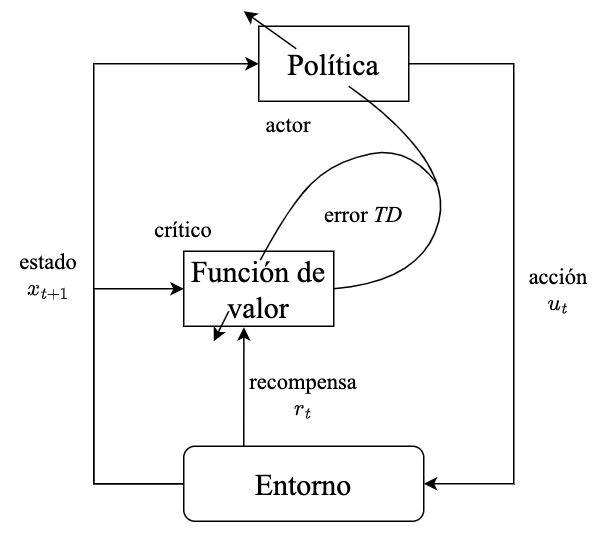
\includegraphics[width=9cm]{05_aprendizaje_por_diferencias_temporales/actor_critic.png}
\caption{Esquema clásico de un método actor-crítico, la política (actor) selecciona acciones que interactúan con el entorno, que devuelve una recompensa y un nuevo estado. Estos son evaluados por la función de valor (crítico), que calcula el error \acrshort{td} y lo manda de regreso a la política para mejorarla. El diagrama esta basado en \cite{Sutton2018}.}
\label{fig:RL_configuration}
\end{figure}

El estructura actor-crítico del método \acrshort{ddpg}
se basa en dos trabajos previos. Para empezar, usa el método \textit{Deterministic Policy Gradient} \cite{silver14} para definir el actor. Así mismo, sigue el algoritmo \textit{Deep Q-Networks} o \textit{Deep Q-learning} \cite{mnih2013} para construir el crítico. 

\subsection{Actor: \textit{Deterministic Policy Gradient}}
\label{subsec:actor}
Este método pertenece a la familia de algoritmos denominados \textbf{gradiente de política} o \textbf{\textit{policy gradient}}, que se basan en la optimización de políticas parametrizadas. El diseño del actor se basa en el ajuste de una red neuronal artificial para construir una política determinista capaz de resolver un problema de control continuo. 

En general, estos algoritmos funcionan a partir del muestreo de una política estocástica y ajustan los parámetros de la política en la dirección de la mayor suma acumulada de recompensas. En principio, se planteo que la política optimizada debía ser estocástica, esto se deriva de los resultados del teorema de gradiente de política. Sin embargo, en \cite{silver14} se demostró la representación determinista de dicho teorema. 

En el planteamiento de este método, el actor esta dado por una política determinista parametrizada por $\bm\theta_{\mu} \in \Theta$. Esta política se denota como $\mu: \mathcal{X}\times\Theta\rightarrow \mathcal{U}$. Con el propósito de optimizar esta política determinista, se utiliza una función desempeño, que se define en términos de las funciones de valor, como se muestra a continuación,
\begin{align}
    J(\bm\theta_{\mu}) &= \mathbb{E}_{\mathbf{x}\sim\rho^{\beta}}\left[V_{\mu}(\mathbf{x})\right] \\
    &= \int_{\mathcal{X}}\rho^{\beta}(\mathbf{x})V_{\mu}(\mathbf{x})d\mathbf{x}\\
    &= \int_{\mathcal{X}}\rho^{\beta}(\mathbf{x})Q_{\mu}(\mathbf{x}, \mu(\mathbf{x};\bm\theta_{\mu}))d\mathbf{x} \\
    &= \mathbb{E}_{\mathbf{x}\sim\rho^{\beta}}\left[
    Q_{\mu}(\mathbf{x}, \mu(\mathbf{x}; \bm\theta_{\mu}))\right].
    \label{eq:dpg_objective}
\end{align}
En este caso $\beta$ denota a la política de comportamiento presentada anteriormente. Esta consideración establece que la configuración de la función \ref{eq:dpg_objective} es \textit{off-policy}. 

Con el propósito de obtener una política que permita acumular el mayor retorno posible, se debe encontrar el mayor valor posible de \ref{eq:dpg_objective}. Esto se logra utilizando el método de gradiente ascendente. Este método de optimización requiere el cálculo del gradiente de la función \ref{eq:dpg_objective} con respecto a $\bm{\theta}_{\mu}$. La existencia del gradiente de \ref{eq:dpg_objective} esta garantizada por el teorema de gradiente de política determinista \cite{silver14}. Este teorema permite expresar el gradiente de la función objetivo \ref{eq:dpg_objective} de la siguiente manera, 
\begin{align*}       \nabla_{\bm\theta_{\mu}}J(\bm\theta_{\mu}) &= \int_{\mathcal{X}} \rho^{\beta}(\mathbf{x}) \nabla_{\mathbf{u}}Q(\mathbf{x}, \mathbf{u})\nabla \mu(\mathbf{x};\bm\theta_{\mu})\big|_{\mathbf{u}=\mu(\mathbf{x};\bm\theta_{\mu})}d\mathbf{x} \\
        &= \mathbb{E}_{\mathbf{x}\sim \rho^{\beta}} 
        \left[
        \nabla_{\mathbf{u}}Q(\mathbf{x}, \mathbf{u})\nabla \mu(\mathbf{x};\bm\theta_{\mu})\big|_{\mathbf{u}=\mu(\mathbf{x};\bm\theta_{\mu})}
        \right].
\end{align*}
A partir de la expresión anterior, se puede establecer la siguiente regla de actualización para los parámetros de la red neuronal, 
    \begin{align}
        \bm\theta^{(k+1)}_{\mu} &= \bm\theta^{(k)}_{\mu} + \alpha_{\mu} \nabla_{\bm\theta_{\mu}}J\left(\bm\theta_{\mu}^{(k)}\right). \label{eq:update_policy_gradient}
    \end{align}

Una vez estimado el actor $\mu$, se procede a a definir su crítico que aproxime a la función de valor $Q_{\mu}$. Esta función de valor resulta fundamental para actualizar $\mu$. Dentro de \acrshort{ddpg} el entrenamiento del crítico se basa en el algoritmo llamado \textit{Deep-Q-learning}, que es una extensión de \textit{Q-learning}.

\subsection{Crítico: \textit{Deep Q-learning}}
\label{sub_sec:DQN}
La estimación que realiza el crítico  se basa en el entrenamiento de una \acrshort{ann} para aproximar la función $Q$, similarmente a como se hizo en \cite{mnih2013}. La gran diferencia radica en que el algoritmo propuesto en \cite{mnih2013} esta planteado para la toma de decisiones sobre un conjunto de acciones discreto. Este planteamiento no es adecuado para las tareas de control. Por lo que se cambia la estructura de \acrshort{ann} asociada al crítico. Concretamente, el crítico se representa por la función $Q:\mathcal{X}\times\mathcal{U}\times\Theta \rightarrow \mathbb{R}$. Esta \acrshort{ann} tiene el propósito de aproximarse a la función de valor acción, como se muestra en la siguiente relación,
\begin{align}\label{eq:Deep_Q_approx}
    Q(\mathbf{x}, \mathbf{u}; \bm\theta_{Q}) \approx
Q_{\mu}(\mathbf{x}, \mathbf{u}).    
\end{align}

Para lograr este propósito, se necesita que la \acrshort{ann} se asemeje a la definición teórica de la ecuación óptima de Bellman. Por ello la función objetivo se compone del valor esperado del error \acrshort{td}, como se muestra en la siguiente expresión,
\begin{align}\label{eq:Q_objective}
    \mathcal{L}\left(\bm{\theta}_Q\right) &= \mathbb{E}_{\mathbf{x}, \mathbf{u}\sim \rho_{\beta}\text{, }\mathbf{x}'\sim p}\left[\left(\underbrace{r(\mathbf{x}, \mathbf{u}) + \gamma \max_{\mathbf{u}'}Q\left(\mathbf{x}', \mathbf{u}';\bar{\bm{\theta}}_{Q}\right)-Q\left(\mathbf{x}, \mathbf{u};\bm{\theta}_{Q}\right)}_{\delta_{t}(\bar{\bm\theta}_{Q}, \bm{\theta}_{Q})}\right)^2\right].
\end{align}

El termino $\bar{\bm\theta}_{Q}$ representa a los parámetros fijados de la actualización anterior. La \acrshort{ann} $Q(\cdot, \cdot; \bar{\bm\theta}_{Q})$ se le denomina \textbf{red de referencia}. Esta red se preserva en la expresión \ref{eq:Q_objective} para estabilizar el aprendizaje \cite{lillicrap2015continuous}. 

En la práctica la función objetivo \ref{eq:Q_objective} 
es difícil de estimar y tiene poca eficiencia en el aprendizaje. Esto se debe a que el valor esperado depende de la distribución de frecuencia de visitas. No obstante, en \cite{mnih2013} se propone como alternativa el uso de un método llamado \textit{\textbf{experience replay}}. Este método consiste que en cada paso $t$ de la simulación se almacena una experiencia $e_t=\left(\mathbf{x}_t, \mathbf{u}_t, r_{t+1}, \mathbf{x}_{t+1}\right)$ dentro de un cache de memoria denotado por $\mathcal{D}$. Posteriormente, se muestrean experiencias almacenadas de manera uniforme, que serán utilizadas para el ajuste de la función $Q$. 

La técnica \textit{experience replay} tiene varias ventajas sobre el planteamiento original. En primer lugar, permite hacer un uso eficiente de las experiencias, ya que al estar almacenadas, estas se pueden usar durante múltiples actualizaciones de la red neuronal. En segundo lugar, el aprendizaje por muestras consecutivas es ineficiente, debido a la fuerte correlación que existe entre las muestras. Tomar uniformemente las muestras permite romper la correlación y reduce la varianza en las actualizaciones. Además permite agrupar a las experiencias en \textit{mini-batches}(mini-lotes) para el ajuste de redes neuronales, una técnica ampliamente utilizada en aprendizaje automático. \cite{mnih2013}

Por otro lado, para definir adecuadamente el error $\delta_{t}^{*}$ en la expresión \ref{eq:Q_objective}, se requiere establecer la siguiente relación,
$$Q(\mathbf{x}, \mu(\mathbf{x};\bm\theta_{\mu}); \bm\theta_{Q}) := \max_{\mathbf{u}'}Q(\mathbf{x}, \mathbf{u}; \bm\theta_{Q}).$$
Esta modificación resulta idónea, ya que $\mu$ tiene la finalidad de aproximarse a la política óptima.

La incorporación de las modificaciones anteriores alteran la función objetivo de la siguiente forma,
\begin{align}
    \mathcal{L}\left(\bm{\theta}_Q\right) &= \mathbb{E}_{(\mathbf{x}, \mathbf{u}, r, \mathbf{x}')\sim U(\mathcal{D}) }\left[\left(r + \gamma Q\left(\mathbf{x}, \mu\left(\mathbf{x};\bar{\bm\theta}_{\mu}\right); \bar{\bm\theta}_{Q}\right) - Q\left(\mathbf{x}, \mathbf{u};\bm{\theta}_{Q}\right)\right)^2\right].
    \label{eq:ddpg_critic_objective}
\end{align}
La optimización de la función \ref{eq:ddpg_critic_objective} se realiza de acuerdo al método de descenso de gradiente, como se expresa en la siguiente actualización, 
\begin{align}
    \bm\theta_Q^{(k+1)} &= \bm\theta_{Q}^{(k)} - \alpha_{Q} \nabla_{\bm\theta_Q} \mathcal{L}\left(\bm\theta_Q^{(k)}\right),
    \label{eq:upadate_Q}
\end{align}
dónde el gradiente $\nabla_{\bm\theta_Q}\mathcal{L}$ se define de la siguiente manera,
\begin{align}
\nabla_{\bm\theta_Q}\mathcal{L}(\bm\theta_Q) &= \mathbb{E}_{(\mathbf{x}, \mathbf{u}, r, \mathbf{x}')\sim U(\mathcal{D}) } 
[\delta_{t}^{*}(\bar{\bm\theta}_{Q}, \bm\theta_Q)\nabla_{\bm\theta_Q}Q(\mathbf{x}, \mathbf{u};\bm\theta_Q)].
\label{eq:ddpg_actor_objective}
\end{align}

\subsubsection{Política de comportamiento}

Un de los mayores retos del aprendizaje en espacios continuos es la exploración \cite{lillicrap2015continuous}. Esto se debe a que no hay un criterio exacto para definir una política de comportamiento adecuada para problemas de control. Los autores del método \acrshort{ddpg} emplean una política de exploración basada en la adición de muestras de ruido de un proceso estocástico a la política determinista $\mu$. La selección de acciones usando la política exploratoria, se puede definir de la siguiente manera, 
\begin{align}
    \mathbf{u}_t = \mu(\mathbf{x}_t;\bm\theta_{\mu}) + \mathcal{O}_t \quad \forall t \in \mathcal{T}, \label{eq:noisy_policy}
\end{align}
dónde $\mathcal{O}_t$  representa una muestra de una proceso estocástico. Los autores de este método proponen usar un proceso de Ornstein-Ulhenbeck. Este proceso permite generar una correlación temporal en la exploración \cite{lillicrap2015continuous}. 

A pesar de que la política de comportamiento depende de la política optimizada $\mu$, el algoritmo sigue siendo \textit{off-policy}. Esto se debe al uso de \textit{experience replay}. Concretamente, el uso de este método permite almacenar experiencias resultantes del uso de la política optimizada de actualizaciones anteriores. Por lo que al momento de actualizar el actor y el crítico, para efectos prácticos, se usa información de distintas políticas. 

\subsection{Algoritmo}
Hasta ahora se esbozado el entrenamiento del actor y el crítico. Ahora se procederá a explicar como se integran ambos elementos dentro del método \acrshort{ddpg}. Antes de comenzar el proceso de aprendizaje, se inicializan de forma aleatoria los parámetros del actor y crítico $\bm\theta_{\mu}$ y $\bm\theta_{Q}$. Y se introducen unas redes neuronales de referencia para estabilizar el aprendizaje el actor y crítico. Los parámetros de la referencia del actor y del crítico son $\bar{\bm\theta}_{\mu}$ y $\bar{\bm\theta}_{Q}$, en el mismo orden. El primer paso que debe realizarse dentro de este algoritmo, consiste en la recolección de experiencias $e_t$ a partir de la interacción entre el entorno y el agente, siguiendo la política de comportamiento $\beta$, es decir, siguiendo la expresión \ref{eq:noisy_policy}. Después de cada interacción se debe guardar la información $e_t$ en la memoria $\mathcal{D}$. Una vez que la memoria tenga por lo menos $N$ experiencias, se muestrean de forma uniforme las $N$ experiencias para entrenar al actor y crítico.

Teniendo un lote de experiencias de tamaño $N$, los parámetros del actor se actualizan de acuerdo a la expresión \ref{eq:update_policy_gradient} donde la expresión $\nabla_{\bm\theta_{\mu}}J$ se estima usando el gradiente de política por muestreo, que se describe de la siguiente forma,
\begin{align}
\nabla_{\bm\theta_{\mu}} J \approx \frac{1}{N}\sum_{i=1}^{N} \nabla_{\mathbf{u}}Q(\mathbf{x},\mathbf{u};\bm\theta_{Q})\Big|_{\mathbf{x}=\mathbf{x}_i, \mathbf{u}= \mu(\mathbf{x}_i)} \nabla_{\bm\theta_{\mu}}\mu(\mathbf{x};\bm\theta_{\mu})\Big |_{\mathbf{x}=\mathbf{x}_i}.
\label{eq:actor_grad}
\end{align}

De la misma forma, los parámetros del crítico se actualizan usando la regla de actualización \ref{eq:upadate_Q}. En este caso la expresión $\nabla_{\bm\theta_{Q}}\mathcal{L}$ se estima usando las muestras del lote proveniente de la memoria $\mathcal{D}$ de la siguiente manera,
\begin{align}
\nabla_{\bm\theta_{Q}}\mathcal{L} \approx \frac{1}{N}\sum_{i=1}^{N}\left(r_{i+1} + \gamma Q\left(\mathbf{x}_{i+1},\mu(\mathbf{x}_{i+1};\bar{\bm\theta}_{\mu});\bar{\bm{\theta}}_{Q}\right)-Q\left(\mathbf{x}, \mathbf{u};\bm{\theta}_{Q}\right)\right)\nabla_{\bm\theta_Q}Q(\mathbf{x}, \mathbf{u};\bm\theta_Q).
\label{eq:critic_grad}
\end{align}
Finalmente, la actualización $k+1$ de las redes de referencia del actor y el crítico se actualizan de forma convexa utilizando los parámetros aprendidos anteriormente. Esto se resume en la expresiones debajo, 
\begin{align*}
    \bar{\bm\theta}_{Q}^{(k+1)} &= \tau \bm\theta_{Q}^{(k+1)} +(1- \tau)\bar{\bm\theta}_{Q}^{(k)}, \\
    \bar{\bm\theta}_{\mu}^{(k+1)} &= \tau \bm\theta_{\mu}^{(k+1)} +(1- \tau)\bar{\bm\theta}_{\mu}^{(k)},
\end{align*}
dónde $\tau << 1$ es un parámetro dado. Esta actualización restringe a que los cambios de los parámetros sea más lento, pero estable. Esto permite transformar el problema de estimar la función de valor $Q$ de un problema relativamente inestable a un caso más parecido al que se tiene en aprendizaje supervisado. \cite{lillicrap2015continuous}  
\begin{algorithm}[h]
    \caption{\textit{Deep deterministic policy gradient} (Lillicrap et at., \cite{lillicrap2015continuous}) }
   % \KwData{política: $\pi$}
   \KwResult{Parámetros optimizados de política $\bm\theta_{\mu}$ y función de valor $\bm\theta_{Q}$.}
    Inicializar aleatoriamente los parámetros de las redes $Q\left(\cdot,\cdot;\bm\theta_Q\right)$ y $\mu\left(\cdot;\bm\theta_{\mu}\right)$.\\
    Inicializar las redes de referencia $Q$ $\mu$ con los parámetros  $\bm\theta_{Q}$, $\bm\theta_{\mu}$, respectivamente. \\
    Inicializar el replay buffer $\mathcal{D}$ \\
    \For{cada episodio}{
        Inicializar el proceso $\mathcal{O}$ para la exploración \\
        Recibir una observación inicial $\mathbf{x}_1$\\
        \For{cada paso $t$ en el episodio}{
            Seleccionar $\mathbf{u}_t = \mu(\mathbf{x}_t ;\bm\theta_{\mu}) + \mathcal{O}$ \\
            Ejecutar acción $\mathbf{u}_t$, observar recompensa $r_t$ y el nuevo estado $\mathbf{x}_{t+1}$ \\
            Almacenar la experiencia $(\mathbf{x}_t, \mathbf{u}_t, r_t, \mathbf{x}_{t+1})$ en $\mathcal{D}$ \\
            Tomar una muestra con un tamaño $N$ de la forma $(\mathbf{x}_i, \mathbf{u}_i, r_i, \mathbf{x}_{i+1})$ de $\mathcal{D}$ \\
            Establecer $y_i = r_i + \gamma Q\left(\mathbf{x}_{i+1}, \mu\left(\mathbf{x}_{i+1};\bar{\bm\theta}_{\mu}\right);\bar{\bm\theta}_{Q}\right)$ \\
            Actualizar el crítico minimizando $\mathcal{L} = \frac{1}{N}\sum(y_i -Q(\mathbf{x}_i, \mathbf{u}_i;\bm\theta_{Q}))^2$ \\
            Actualizar el actor usando el gradiente de política por muestreo, 
            $$\nabla_{\bm\theta_{\mu}} J \approx \frac{1}{N}\sum_{i} \nabla_{\mathbf{u}}Q(\mathbf{x},\mathbf{u};\bm\theta_{Q})\Big|_{\mathbf{x}=\mathbf{x}_i, \mathbf{u}= \mu(\mathbf{x}_i)} \nabla_{\bm\theta_{\mu}}\mu(\mathbf{x};\bm\theta_{\mu})\Big |_{\mathbf{x}=\mathbf{x}_i}$$ \\
            Actualizar los parámetros de las redes de referencia:
            \begin{align*}
    \bar{\bm\theta}_{Q} &\leftarrow \tau \bm\theta_{Q} +(1- \tau)\bar{\bm\theta}_{Q}, \\
    \bar{\bm\theta}_{\mu} &\leftarrow \tau \bm\theta_{\mu} +(1- \tau)\bar{\bm\theta}_{\mu}.
\end{align*}
        }
        \label{alg:DDPG}
    }\end{algorithm}



\chapter{Aplicación y evaluación de métodos RL}


\section{Planteamiento del problema}

El objetivo de control que se planteó es simple. Diseñar una política de control que desde una posición  y velocidad inicial aleatoria, contenida en una cierta región del espacio de configuración, guíe al cuadricoptero a una posici\'on determinada que sin perder generalidad asumimos es el origen. La política de control consiste en una \acrshort{ann}, cuyos parámetros se entrenaron usando un esquema de aprendizaje por refuerzo. 

En el modelo de aprendizaje se definieron los estados del sistema como un vector de tamaño 12 que consiste de las velocidades lineales, velocidades angulares y la posición del cuadricoptero (centro de masa y ángulos de Euler). Al igual que en el trabajo \cite{hwangbo2017control} para la implementación resultó más conveniente usar la representación de las coordenadas angulares en términos de la la matriz de rotación \ref{eq:rotation_matrix} por lo que el estado del sistema consiste en un vector de 18 entradas, aunque únicamente 12 son independientes.  
Las acciones de la política de control están dadas por las cuatro velocidades angulares de los motores del cuadricoptero, como se describe en  \ref{sec:quadcoper_control_system}.
\subsection{Configuración del entorno}
Para simular la evolución discreta de estados del entorno del cuadricoptero de la forma,
\begin{align}
    \mathbf{x}_{t+1}=f(\mathbf{x}_t, \mathbf{u}_t) \quad \forall t\geq0
    \label{eq:discrete_f}
    \end{align}
se resuelve numéricamente el sistema de ecuaciones diferenciales ordinarias dada por las \crefrange{eq:u}{eq:z}. En particular se utilizó la la función \textit{scipy.integrate.odeint} en Python. Esta función resuelve problemas de valor inicial utilizando Lsoda de la biblioteca de FORTRAN odepack. 

En principio el tiempo de simulación es de 30 segundos, donde cada paso de simulación es un intervalo $\Delta t=0.04$ segundos lo que equivale $T=750$ pasos de tiempo. 

\begin{figure}[h!]
\centering
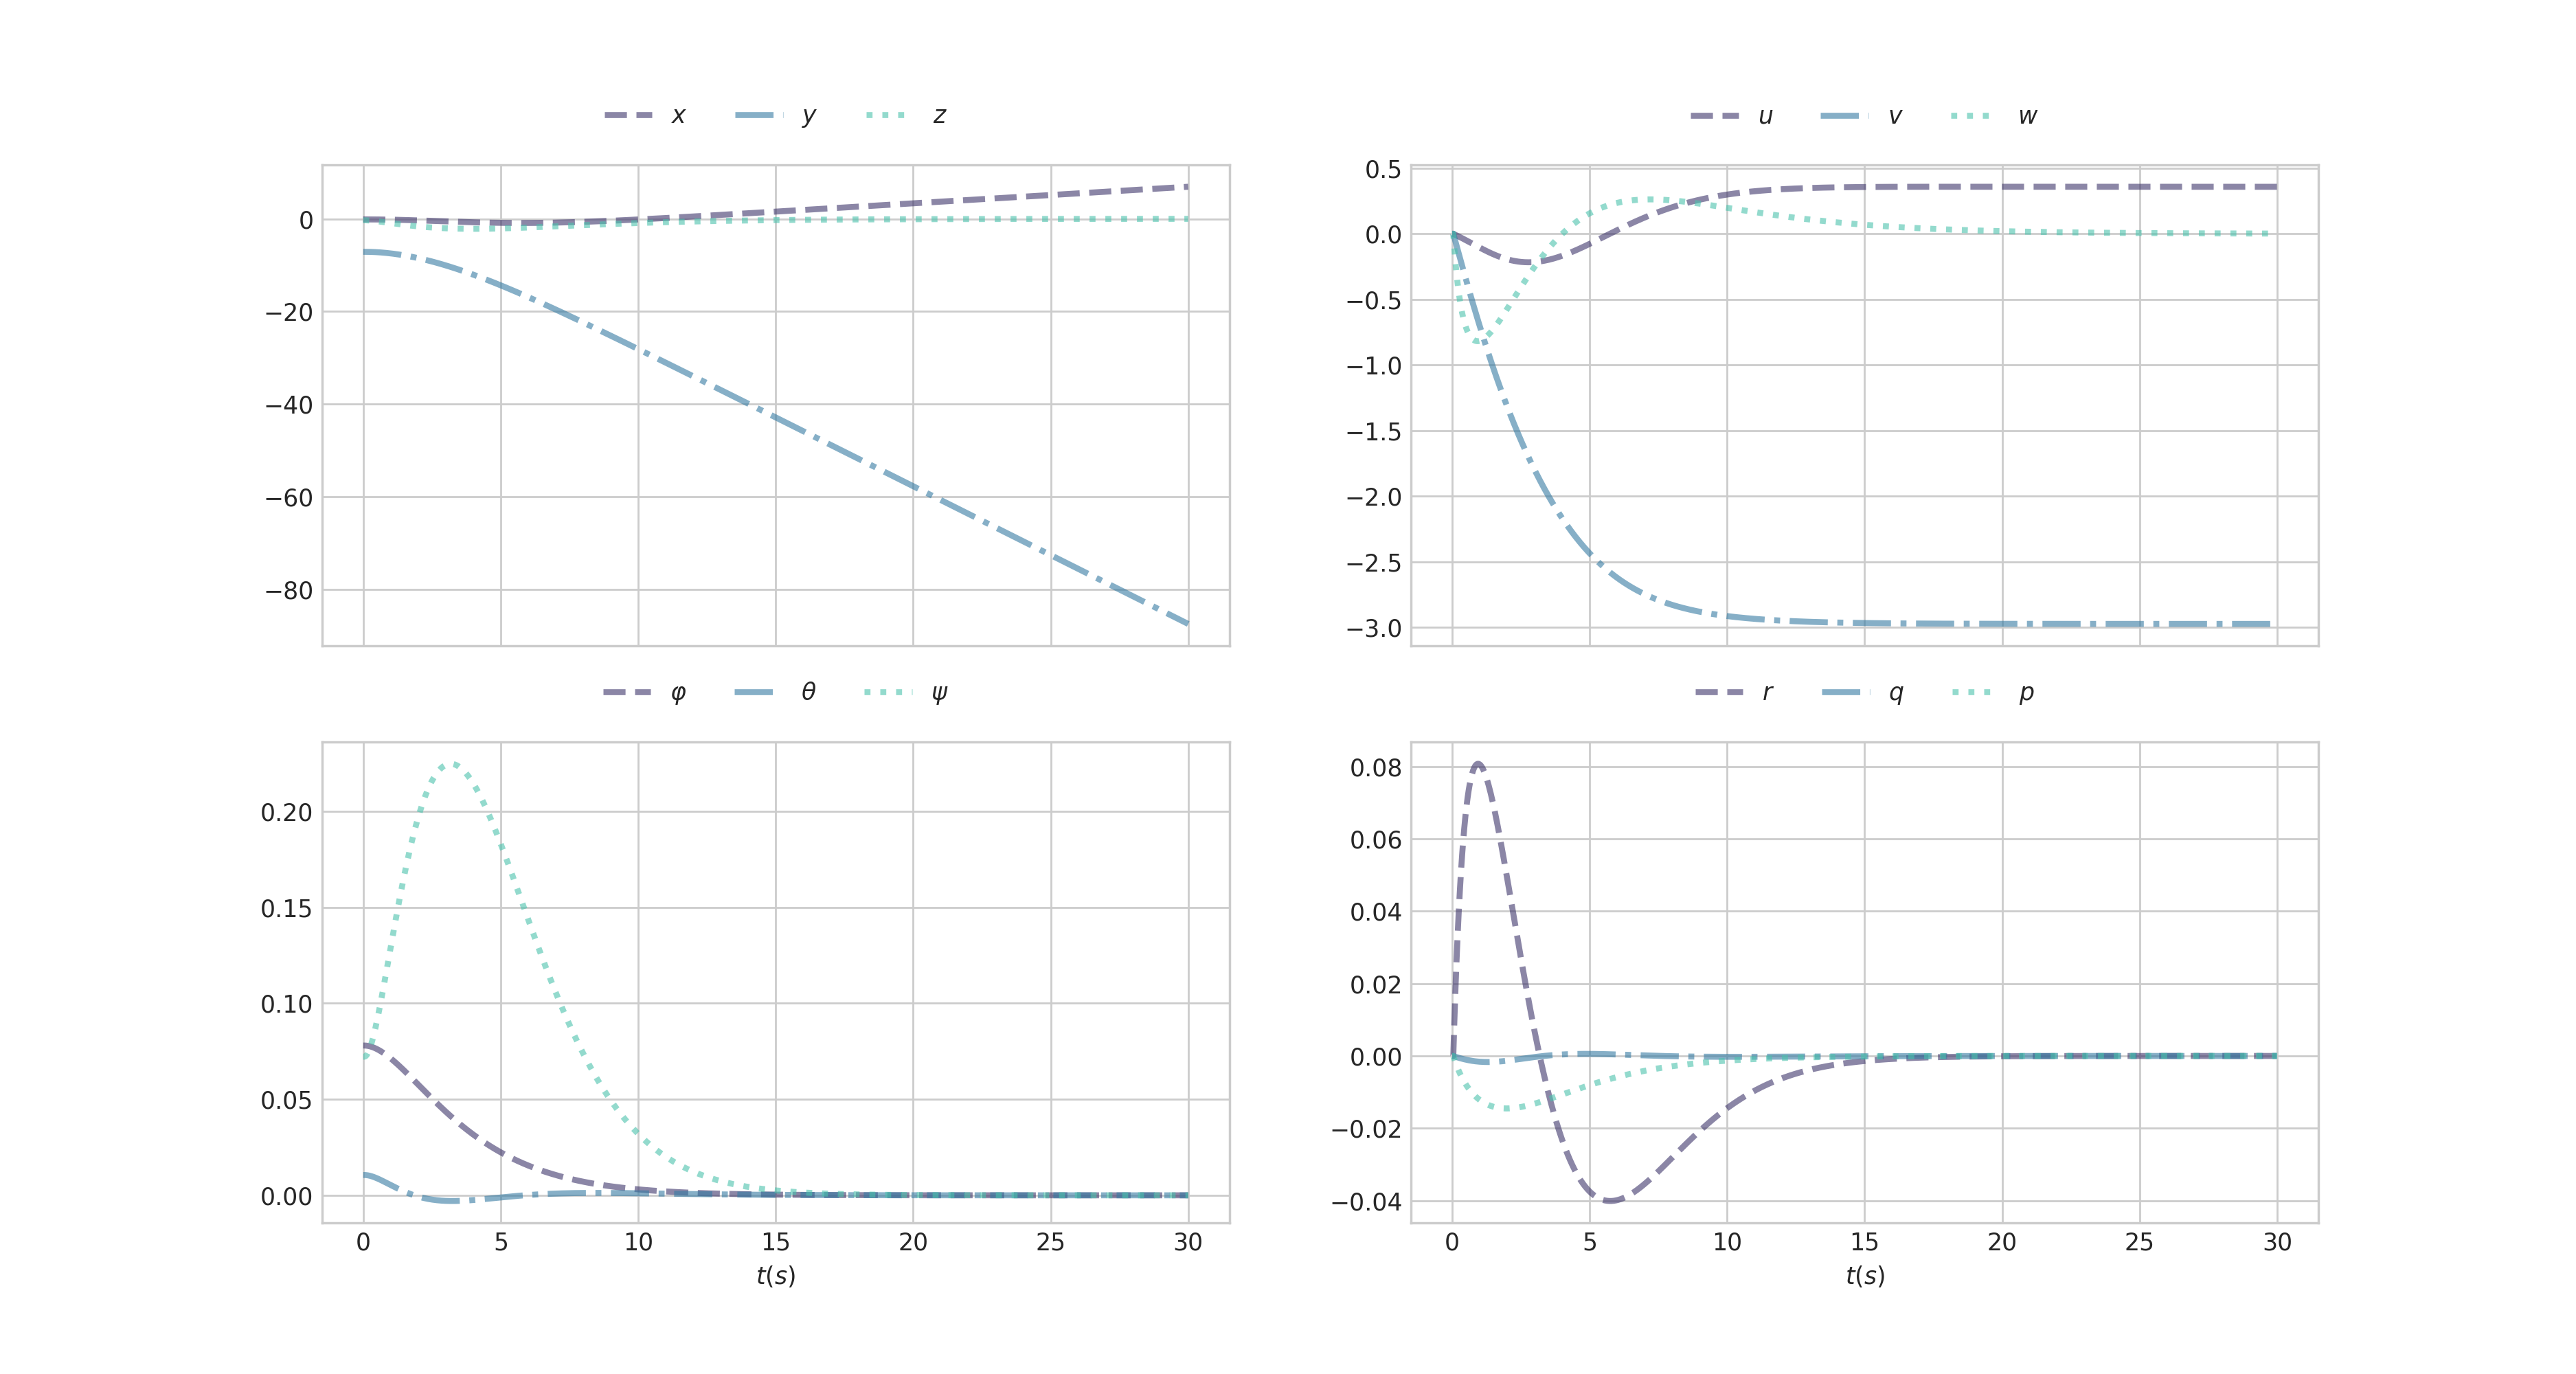
\includegraphics[width=1.0\linewidth]{06_aplicacion_y_evaluacion_de_metodos_rl/linear_states.png}
\caption{Muestra de evolución de coordenadas inerciales $(x, y, z, \phi, \theta, \psi)$ y velocidades locales $(u, v, w, p, q, r)$ simuladas con \ref{eq:discrete_f} bajo algoritmo de control por retroalimentación \ref{alg:Control_retro}.}
\label{fig:gps_schema}
\end{figure}



\subsection{Función de costo y recompensa}

\subsubsection{Diseño de costo para \acrshort{gps}}
Para especificar por completo el uso de los algoritmos usados en este trabajo es necesario definir una función de costo y recompensa. En el caso del método \acrshort{gps}, la expresión que define al costo es, 
\begin{align}
c(\mathbf{x}, \mathbf{u}) = c_1\cdot\|\bm\xi\|_2 + c_2\cdot \|\bm\nu\|_2 + c_3 \cdot \|\bm\omega\|_2 + c_4 \cdot \|\mathbf{I}_{3} - \mathbf{R}(\bm{\eta})\|_2 + c_5 \cdot \|\mathbf{u}\|_2,
\label{eq:cost_quadcopter}
\end{align}
dónde $\bm\xi$, $\bm\eta$, $\bm\nu$ $\bm\omega$ representan la posición, la orientación, la velocidad lineal y la velocidad angular del cuadricoptero, respectivamente. La función $\mathbf{R}$ representa el mapeo de ángulos $\bm\eta$ a la correspondiente matriz de rotación de Euler \ref{eq:rotation_matrix}.  Estas expresiones fueron descritas en las ecuaciones \ref{eq:position_intertial_system} y \ref{eq:position_local_system}. 

La estructura del costo \ref{eq:cost_quadcopter} está diseñada para inducir el comportamiento para cumplir el objetivo fijado, mantener al cuadricoptero en la posición origen, alineado con los ejes y con velocidades angulares y lineales iguales a cero. 

La expresión \ref{eq:cost_quadcopter} queda completamente definida al escoger los valores de los parámetros $c_1, c_2, c_3$, $c_4$ y $c_5$. Para hacer esta elección, se optimizaron varios controladores con el método \acrshort{ilqr} variando los parámetros de \ref{eq:cost_quadcopter}. Se utilizó la implementación de este método del repositorio \cite{ilqr2019}, así como los hiperparámetros preestablecidos. 

Posteriormente bajo cada controlador se simularon 1000 trayectorias del cuadricoptero, donde cada condición inicial se obtiene fijando las velocidades en cero y cambiando uniformemente las coordenadas de la posición $\bm\xi$ y la orientación $\bm\eta$, tal como se describe en el siguiente conjunto,
\begin{align}
    \mathcal{X} = \left\{[x, y, z, 0, 0, 0, 0, 0, 0, \varphi, \theta, \psi] |\quad x \sim \mathcal{U}(x_{-}, x_{+})\text{, } y \sim \mathcal{U}(y_{-}, y_{+})\text{, }\cdots\text{, }\psi \sim \mathcal{U}(\psi_{-}, \psi_{+})\right\}.
    \label{eq:set_initial_conditions}
\end{align}
Los parámetros de las distribuciones del conjunto \ref{eq:set_initial_conditions} utilizados se encuentran en la tabla \ref{tab:reward_set_tests}.

\begin{table}[h]
\centering
\begin{tabular}{|l|l|l|l|l|l|}
\hline
 $x$ & $y$  &$z$  &$\varphi$  &$\theta$  &$\psi$  \\ \hline
 $\pm8$&  $\pm8$& $\pm8$ &$\pm\frac{\pi}{32}$  &$\pm\frac{\pi}{32}$  &$\pm\frac{\pi}{32}$  \\ \hline
\end{tabular}
\caption{Rangos de las distribuciones uniformes del  conjunto \ref{eq:set_initial_conditions}.}
\label{tab:set_initial_conditions}
\end{table}
 El criterio que se uso para determinar el mejor grupo de constantes $\{c_i\}$, consistió en identificar el conjunto que consiga la menor dispersión con respecto al origen de la norma del supremo sobre el estado final $\mathbf{x}_{T}$ de cada trayectoria simulada. Para ejemplificar la variabilidad de esta dispersión se muestran tres conjuntos de parámetros en la tabla \ref{tab:reward_set_tests}. Se eligió el conjunto número dos ya que fue el que obtuvo mejor resultado como se observa en la figura \ref{fig:reward_density}. Para este conjunto los percentiles $5\%$ y $95\%$ se encuentra en los valores de 0.02 y 0.80, respectivamente.


\begin{table}[h!]
\centering
\begin{tabular}{|c|c|c|c|}
\hline
\multirow{2}{*} & \multicolumn{3}{c|}{Conjunto} \\ \cline{2-4}
 & 1  &  2 & 3 \\ \hline
$c_1$ & 0.1& 10 & 10 \\
$c_2$ & 0.01& 10 & 10\\
$c_3$ & 0.01& 10 & 10\\
$c_4$ & 0.05& 100 & 10\\
$c_5$ & 0.005& 0.5 & 10\\
\hline
\end{tabular}
\caption{Configuraciones de parámetros del costo \ref{eq:cost_quadcopter}}
 \label{tab:reward_set_tests}
\end{table}

\begin{figure}[h!]
\centering
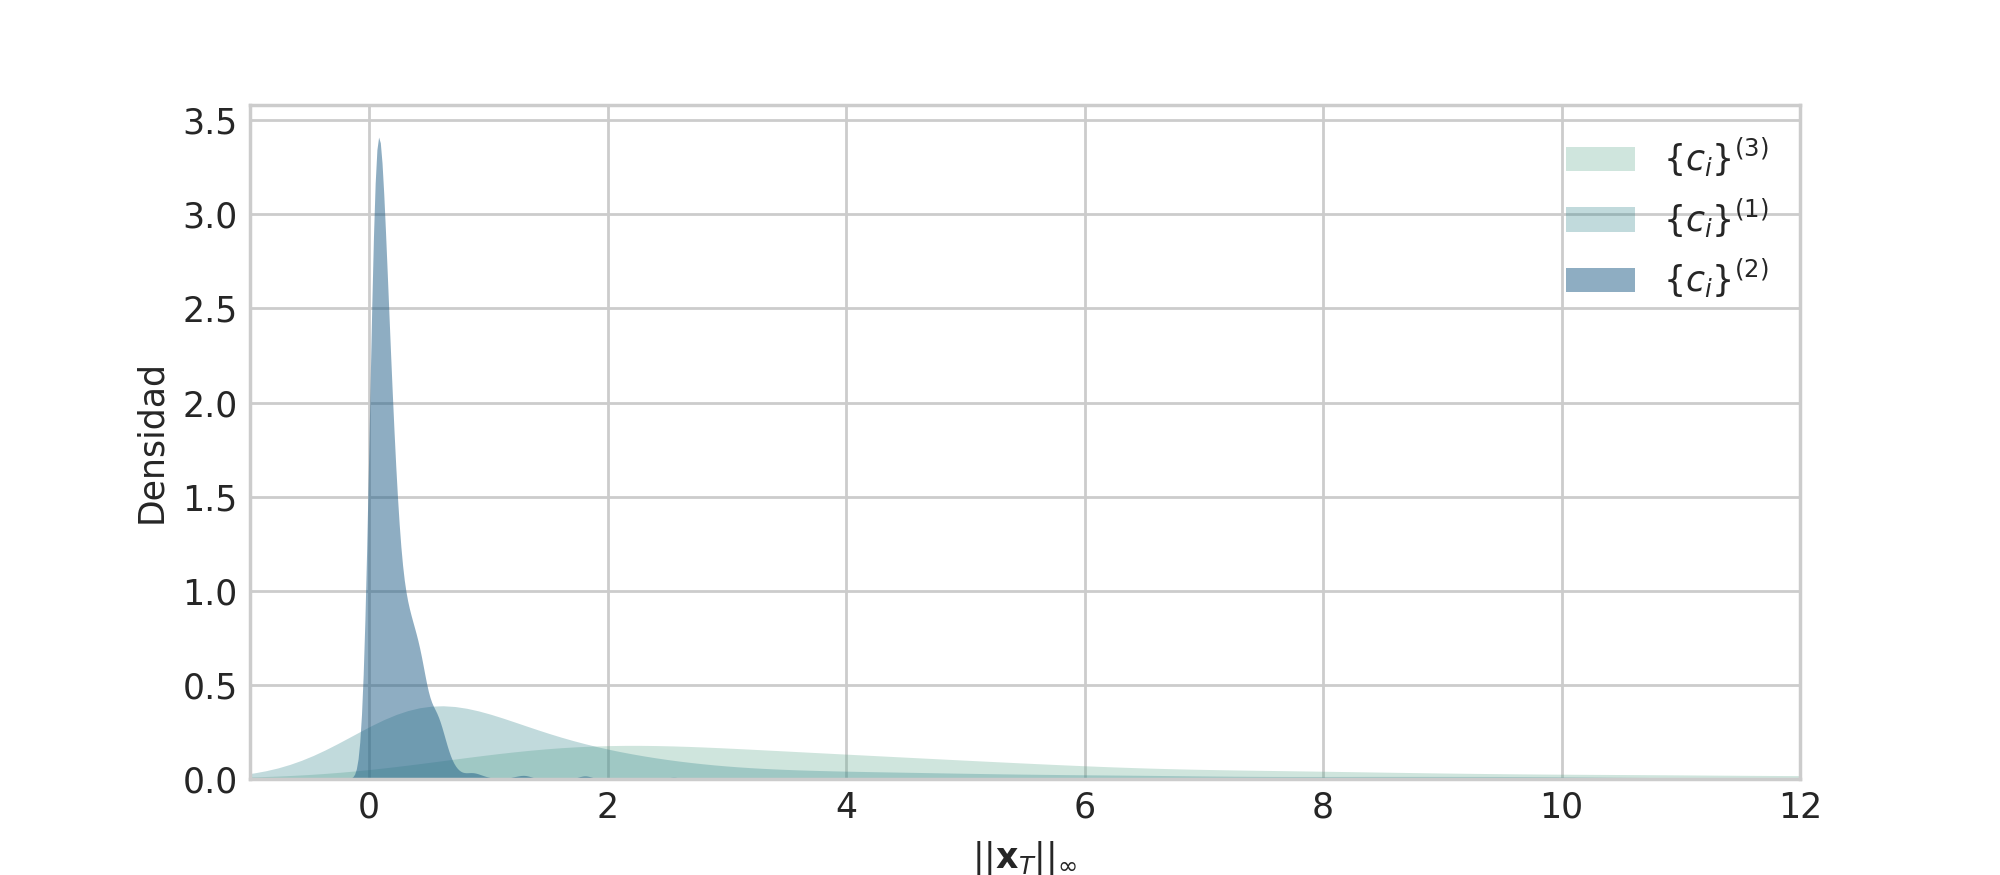
\includegraphics[width=0.8\linewidth]{06_aplicacion_y_evaluacion_de_metodos_rl/test_distribution.png}
\caption{Estimación densidad de la norma del supremo de $\mathbf{x}_{T}$ bajo los diferentes controladores \acrshort{ilqr} ajustados con las configuraciones de parámetros del cuadro \ref{tab:reward_set_tests}}
\label{fig:reward_density}
\end{figure}

A pesar de que se encontró una configuración del costo que hace que el controlador sea efectivo en su funcionamiento, no se puede afirmar que se eligió una configuración óptima. La optimización de estos parámetros trasciende el propósito de este trabajo por lo que no se indagará más.

\begin{figure}[H]
\centering
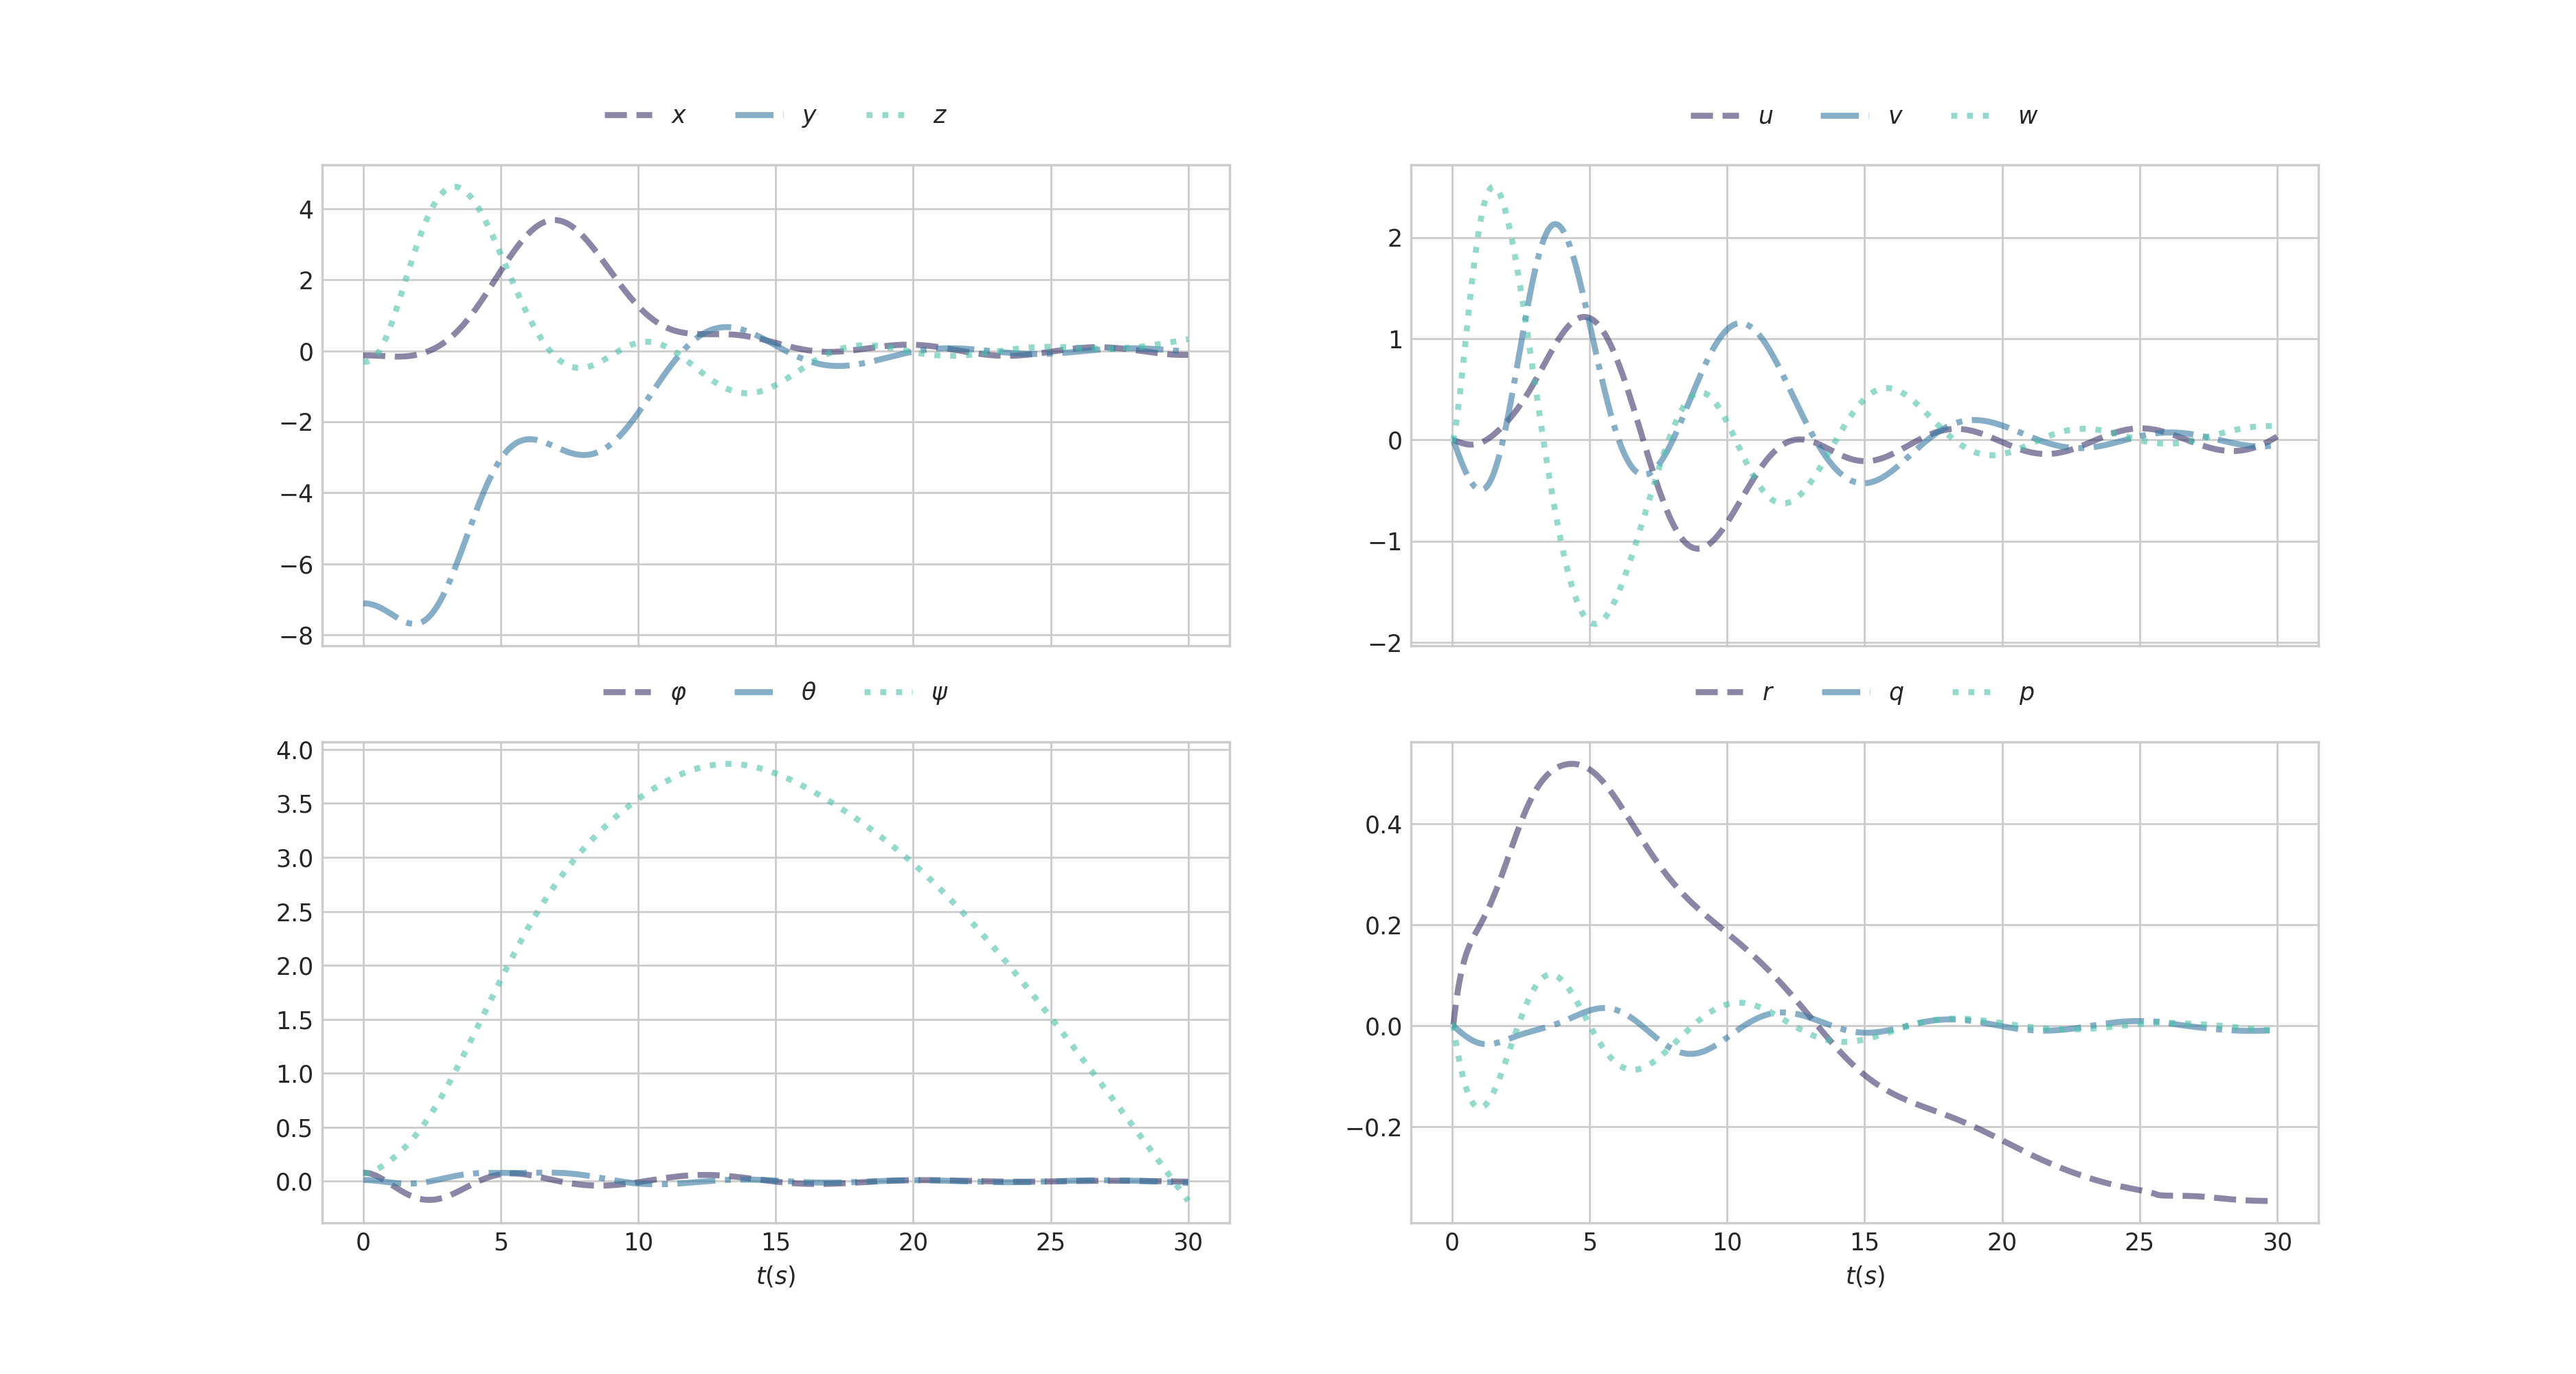
\includegraphics[width=1.0\linewidth]{06_aplicacion_y_evaluacion_de_metodos_rl/ilqr_states.png}
\caption{Muestra de evolución de coordenadas inerciales $(x, y, z, \phi, \theta, \psi)$ y velocidades locales $(u, v, w, p, q, r)$ simuladas con \ref{eq:discrete_f} bajo algoritmo \acrshort{ilqr} \ref{alg:ilqr} con la configuración 2 del costo \ref{eq:cost_quadcopter}.}
\label{fig:state_traj_ilqr}
\end{figure}

\begin{figure}[H]
\centering
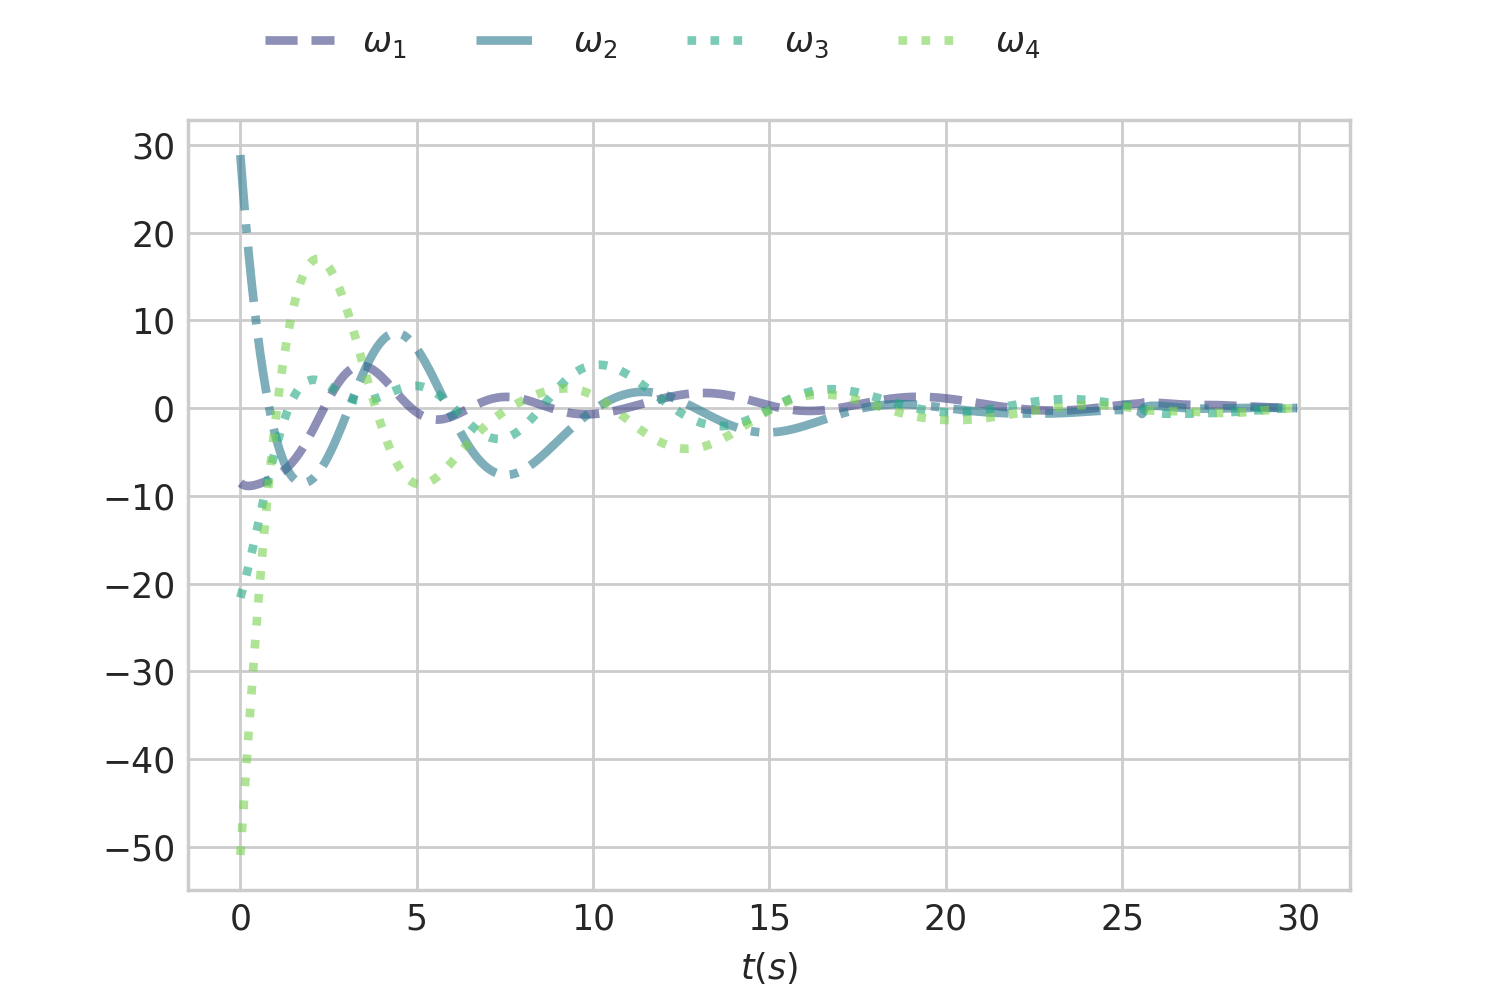
\includegraphics[width=0.6\linewidth]{06_aplicacion_y_evaluacion_de_metodos_rl/ilqr_actions.png}
\caption{Velocidad de rotores $(\omega_1, \omega_2, \omega_3, \omega_4)$ generadas por el controlador \acrshort{ilqr} asociadas a la trayectoria de estado mostrado en la figura \ref{fig:state_traj_ilqr}.}
\end{figure}

\subsubsection{Diseño de recompensa \acrshort{ddpg}}
Debido a que la forma funcional de la recompensa puede ser mucho más libre para el método \acrshort{ddpg} no tiene que tener estrictamente un signo como \acrshort{gps}. Se diseñó una función 
incentive de forma continua al agente a cumplir el objetivo, mientras que cuando este lejos de la región de interés sea penalizado. La función descrita anteriormente esta dada por,  
\begin{align*}
r(\mathbf{x},\mathbf{u}) = r_1({x,y,z}) + r_2(\psi,\theta,\psi) + r_{3}(x, y, z),
\end{align*}
donde,
\begin{align}
    r_1(x, y, z) &= 5 - 5 \cdot \tanh^2\left(\| [x, y, z] \|_2\right), \label{eq:reward_1}\\ 
    r_2(\psi, \theta, \varphi) &= 1 - \tanh^2\left(\| \mathbf{I}_3 - \mathbf{R}(\psi, \theta, \varphi) \|_2 \right), \label{eq:reward_2}\\
    r_3(x, y, z) &= \begin{cases}  
-100 & \text{Si }\exists i \in \{x,y,z\} : i < -8 \lor i > 8 \\
0 & \text{e.o.c}
\end{cases}. \label{eq:reward_3}
\end{align}
El propósito de las funciones \ref{eq:reward_1} y \ref{eq:reward_2} es premiar continuamente al agente cuando la posición inercial del  cuadricoptero esta cerca del origen. En cambio la función \ref{eq:reward_3} tiene la finalidad de penalizar a el agente cuando logra que el cuadricoptero este fuera del espacio de $8\times8\times8$ metros alrededor del origen. 

\section{Proceso de entrenamiento}

La implementación de los métodos \acrshort{gps} y \acrshort{ddpg} requiere de la elección de algunos hiperparámetros que están fuera del modelo de aprendizaje. En esta sección se describirán estos algoritmos por medio de un diagrama, haciendo énfasis en los valores de los hiperparametros que se escogieron. 

\subsection{\acrlong{gps}}
Para utilizar el método de \acrlong{gps}, primero es necesario obtener $N$ distintos controladores ajustados con el método \acrshort{ilqr} usando el costo \ref{eq:cost_quadcopter}. En este trabajo se ajustó un controlador inicial a partir de una trayectoria generada con el algoritmo \ref{alg:Control_retro} de control por retroalimentación, empleando como estado inicial el origen. Posteriormente, con este controlador inicial, se obtuvieron $N$ trayectorias comenzando en estados cercanos al origen dentro del conjunto $\mathcal{X}$ \ref{eq:set_initial_conditions}. Estas trayectorias se usaron para ajustar los $N$ controladores $p_i$, que serán empleados en el ciclo de entrenamiento de la política global $\pi_{\bm{\theta}}$. La \acrshort{ann} asociada a la política global se inicializa con parámetros aleatorios.

Tomando de referencia el trabajo \cite{zhang2016} se realizaron $K=5$ iteraciones de búsqueda guiada de política. Por otra parte se consideraron en este trabajo se $N=7$ controladores, incluyendo uno con una trayectoria con posición inicial en el origen y por cada controlador se simularon $M=800$ trayectorias en cada iteración.


\begin{figure}[h!]
\centering
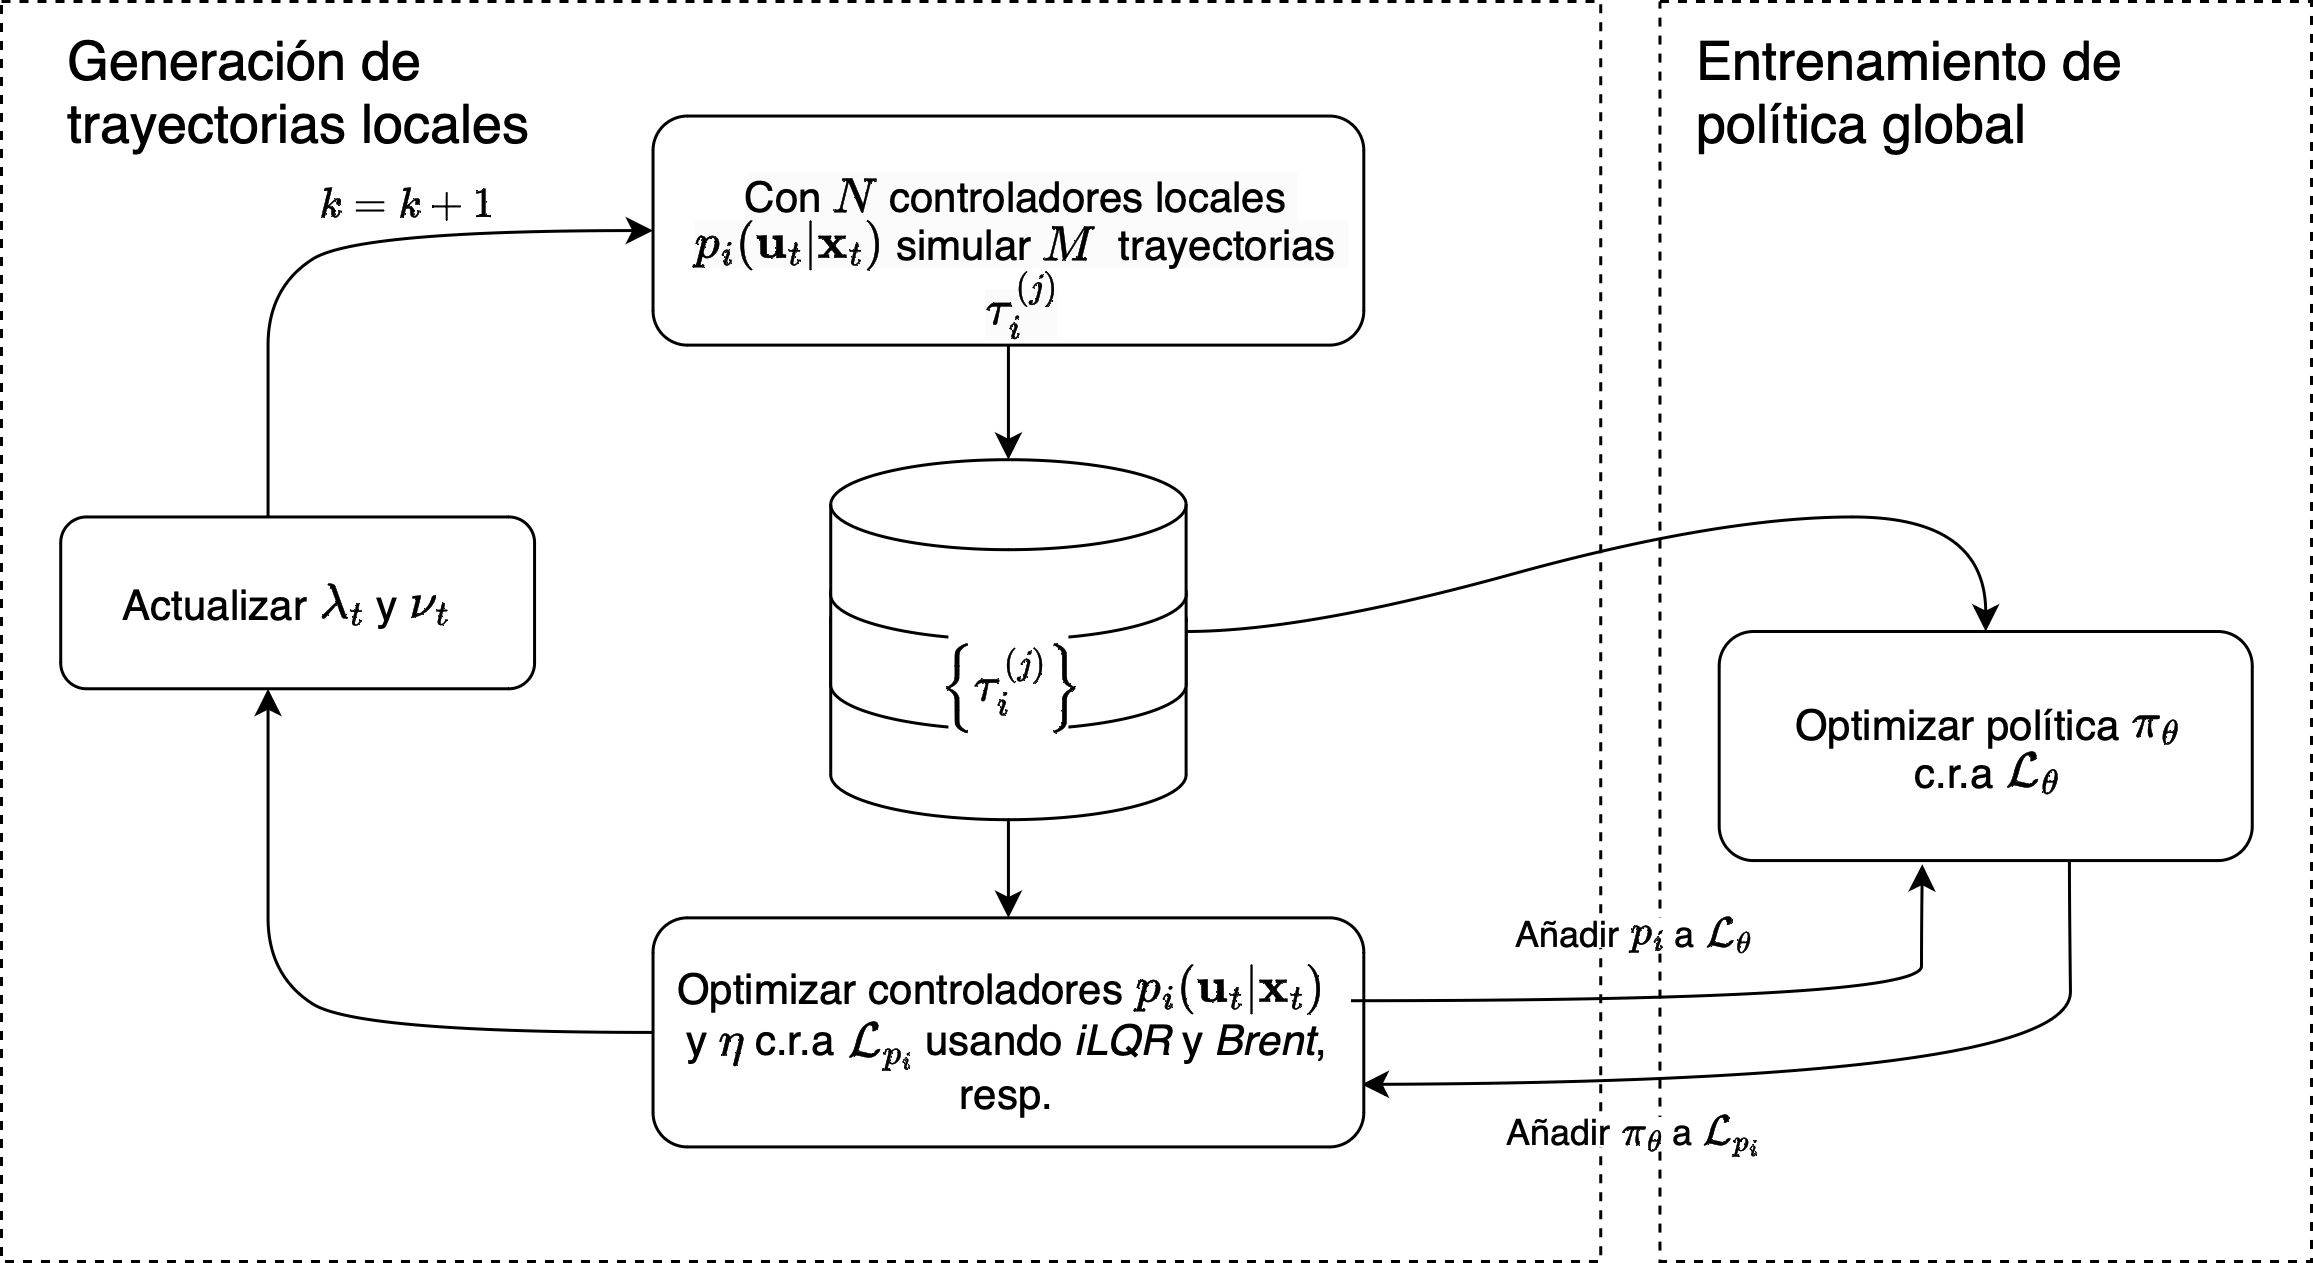
\includegraphics[scale=0.6]{06_aplicacion_y_evaluacion_de_metodos_rl/gps_algorithm.png}
\caption{Esquema de búsqueda guiada de política.}
\label{fig:gps_schema}
\end{figure}

El ciclo de entrenamiento se muestra en la figura \ref{fig:gps_schema}. En cada iteración del ciclo de entrenamiento se comienza con la generación de $M$ trayectorias distintas por cada uno de los $N$ controladores. Las $M \cdot N$ trayectorias son procesadas de tal forma que pueda ser optimizada la política global $\pi_{\bm\theta}$ con respecto a la función objetivo $\mathcal{L}_{\bm\theta}$, como se muestra en la expresión \ref{eq:policy_theta_sim}. Para la optimización se utilizó la implementación en Pytorch del método \acrshort{adam}\footnote{Es un algoritmo de optimización estocástica de primer orden basado en gradientes \cite{ADAM2017}. Es una variante adaptativa del método descenso de gradiente, explicado en \ref{sec:gradient_decent}} con tasa de aprendizaje $\alpha=\text{0.01}$. Una vez actualizada la política global, ésta se añade al costo que será utilizado para ajustar los nuevos $N$ controladores locales. 

Posteriormente se optimiza la transformación de la variable dual $\log(\eta)$ con respecto a $\mathcal{L}_{p_i}$ usando el método de Brent. El valor inicial es $0$, mientras que el rango de búsqueda esta entre los valores $\log(10^{-4})$ y $\log(10^{4})$. 

Para actualizar los valores $\bm\lambda_{t}$ se hace una estimación empírica de la expresión \ref{eq:GPS_lambda} utilizando las $M \cdot N$ trayectorias recolectadas en la iteración. En este caso se utiliza la tasa $\alpha_{\bm\lambda}=\text{0.01}$. 

La actualización de los multiplicadores $\nu_t$ se realiza siguiendo el esquema presentado en \cite{Deep_Visuomotor_Policies}. Se estableció un valor inicial $\nu_{t}=\text{0.001}$ para cada $t$. En cada iteración, se calcula la media y la desviación de la divergencia \acrshort{kl} entre $p(\mathbf{u}_t|\mathbf{x}_t)$ y $\pi_{\bm\theta}(\mathbf{u}_t|\mathbf{x}_t)$ en cada paso de tiempo \cite{Deep_Visuomotor_Policies}. Los valores $\nu_t$ que correspondan a pasos de tiempos donde la divergencia \acrshort{kl} sea más grande que el promedio, será incrementado por un factor de $2$ \cite{Deep_Visuomotor_Policies}. En cambio, en los valores correspondientes a los pasos de tiempo donde la divergencia \acrshort{kl} este por debajo de dos desviaciones estándar, serán reducidos por un factor de $2$ \cite{Deep_Visuomotor_Policies}. 

Para la política $\pi_{\bm\theta}$ se utilizó una \acrshort{ann} con arquitectura de dos capas ocultas de 128 neuronas cada una con función de activación \acrshort{relu}. La \acrshort{ann} tiene una capa de salida de 4 valores correspondientes a las variables de control $\mathbf{u}_t$. Se le aplica la función tangente hiperbólica y se transforman los valores usando la siguiente expresión, 
\begin{align}
\mathbf{u}_t^{\pi} = \frac{\omega_{\max} - \omega_{\min}}{2} \, \mathbf{a}_t + \frac{\omega_{\max} + \omega_{\min}}{2},
\qquad \mathbf{a}_t \in [-1, 1]^4, \; \mathbf{u}_t^{\pi} \in [\omega_{\min}, \omega_{\max}]^4,
\label{eq:action_transformation}
\end{align}
donde $\mathbf{a}_{t}$ representa la salida de la \acrshort{ann}. En este caso se estableció que la acción mínima y máxima son $\omega_{\min}=-\text{0.6}\cdot\omega_{0}$ y $\omega_{\max}=\text{0.6}\cdot\omega_{0}$, respectivamente. 

\subsection{\acrlong{ddpg}}
\label{sec:train_ddpg}

La implementación del algoritmo \acrshort{ddpg} usada en este trabajo se basa en la biblioteca \textit{Spinning Up} de \textit{OpenAI}. Para empezar a usar este algoritmo sólo se requiere inicializar los parámetros de las \acrshort{ann} del actor $\bm\theta_{\mu}$ y del crítico $\bm\theta_Q$ de forma aleatoria. Se asigna un copia de estos valores a parámetros de de referencia $\bar{\bm\theta}_{\mu}$ y $\bar{\bm\theta}_Q$. Para el actor se utilizó la misma configuración que la política global en \acrshort{gps}, así como la transformación \ref{eq:action_transformation}. Mientras que para el crítico se retoma esta misma arquitectura con la uníca excepción de la última capa, en ese este caso no se aplica función de activación y sólo tiene una dimensión el valor de salida. Se inicializa un buffer $\mathcal{D}$ vacío con una capacidad máxima de $10^5$. 

Para no saturar $\mathcal{D}$ de experiencias que no correspondan al objetivo y así facilitar el aprendizaje en la región deseada, se optó por terminar los episodios de entrenamiento cuando el cuadricoptero este fuera de la región $10\times10\times10$ metros alrededor del origen.

\begin{figure}[h!]
\centering
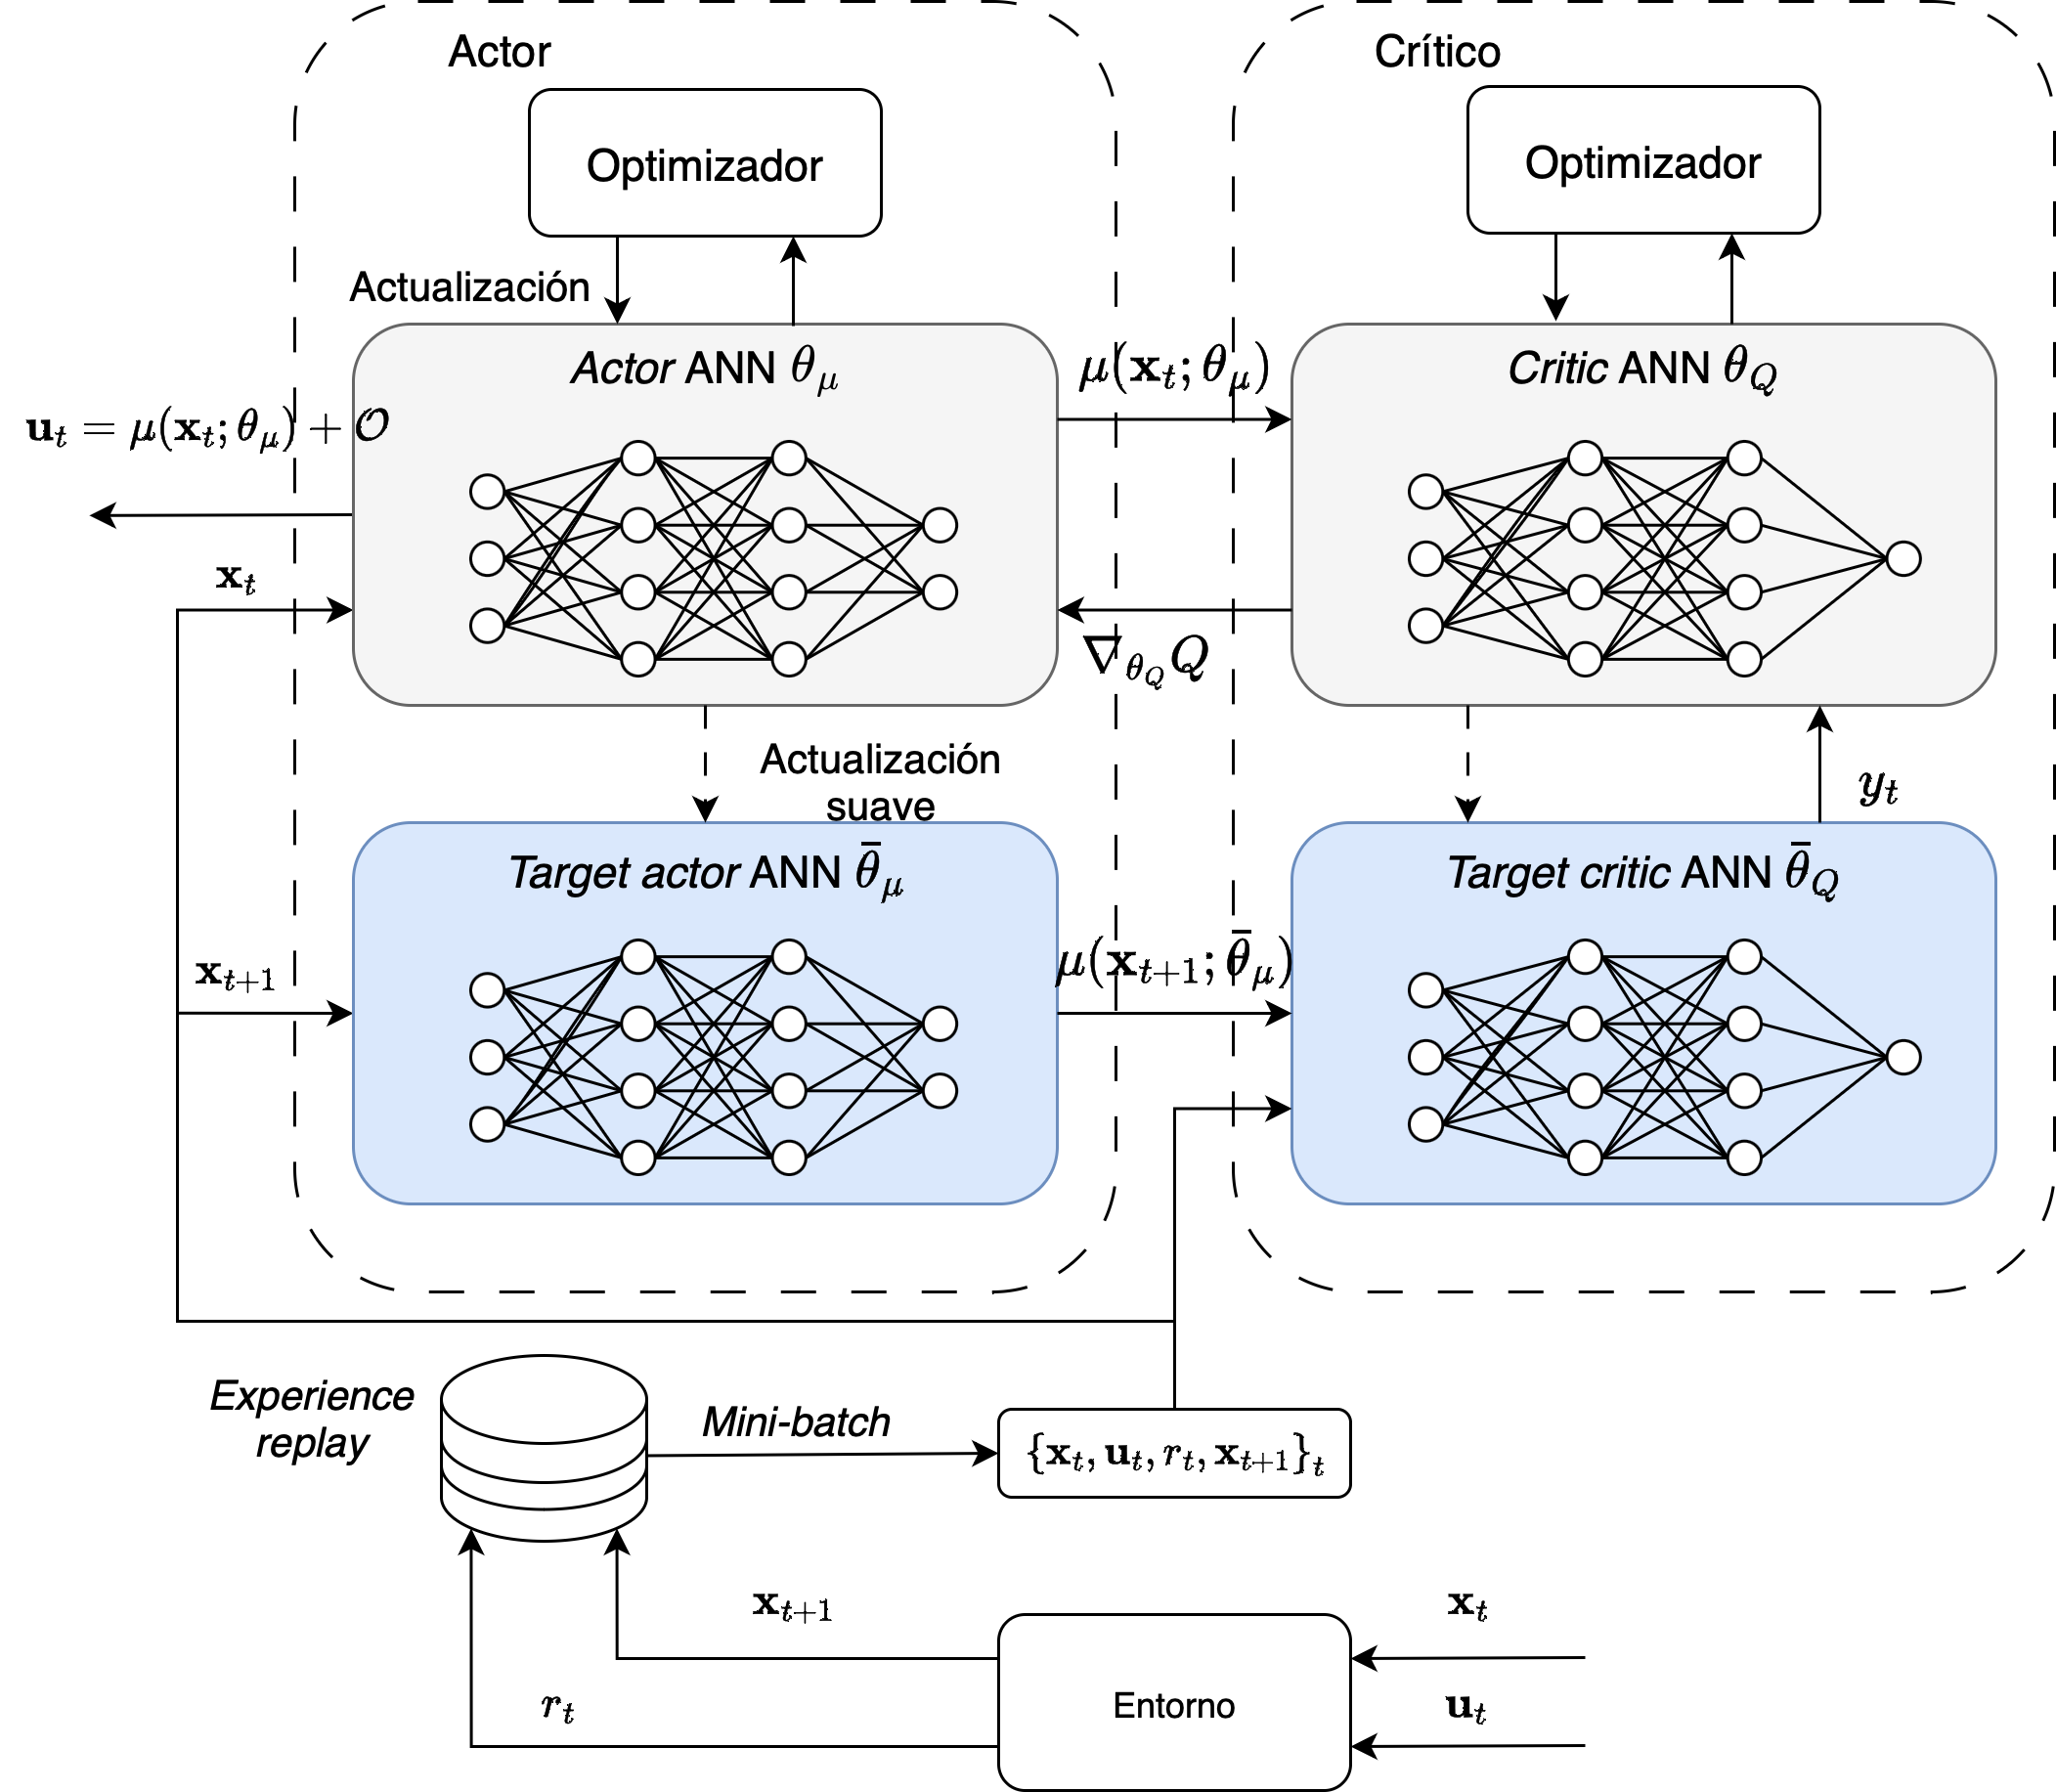
\includegraphics[scale=0.6]{06_aplicacion_y_evaluacion_de_metodos_rl/ddpg_algorithm.png}
\caption{Esquema de \acrshort{ddpg} basado en \cite{jeng23}.}
\label{fig:ddpg_schema}
\end{figure}

Se realizaron 10 \textit{epochs} de entrenamiento, cada \textit{epoch} equivale a realizar $K=5$ episodios con una cantidad máxima de $T=750$ pasos de tiempo. Cada episodio empieza con el muestreo de una posición inicial $\mathbf{x}_1 \in \mathcal{X}$ (conjunto definido en la expresión \ref{eq:set_initial_conditions}). A partir de esta posición inicial se simula un episodio, en cada paso de tiempo se toma una acción a partir de la combinación de la salida del actor y el ruido $\mathcal{O}$, cuya configuración esta definida en \ref{tab:ou_noise}. A partir de la acción ruidosa se observan la recompensa y estado $r_t$, $\mathbf{x}_{t+1}$. Posteriormente, se alamacena la experiencia $(\mathbf{x}_{t}, \mathbf{u}_t, r_t, \mathbf{x}_{t+1})$ en $\mathcal{D}$. Cuando el $\mathcal{D}$ tenga la cantidad suficiente de experiencias se muestrea un \textit{mini-batch} de tamaño $N$ para calcular los gradientes $\nabla _{\bm{\theta}_{\mu}}J$ \ref{eq:actor_grad} y $\nabla_{\bm\theta_{Q}}\mathcal{L}$ \ref{eq:critic_grad} para optimizar $\bm\theta_{\mu}$ y $\bm\theta_{Q}$, los parámetros del actor y crítico, respectivamente. Para la optimización de las redes se utilizó \acrshort{adam}, se retomaron de \cite{singh19} los valores $\alpha_{\mu}=10^{-3}$ y $\alpha_{Q}=$ $10^{-4}$. También de \cite{singh19} se recuperaron los valores $\gamma=0.99$, $\tau=10^{-3}$ y $N=128$. 

\section{Resultados}
Esta sección comienza con la descripción de los resultados de optimización de distintas políticas usando los métodos \acrshort{ddpg} y \acrshort{gps}. Posteriormente, se mostrará un análisis de la estabilidad en trayectorias de vuelo con condiciones iniciales distintas a las usadas en el entrenamiento con la finalidad de evaluar la confiabilidad de estos métodos.

\subsection{Resultados de entrenamiento \acrshort{gps}}
Para validar la optimización de la política global al final de cada iteración de entrenamiento se realizaron $M=800$ trayecotorias de prueba con la configuración resultante de la \acrshort{ann}. Se calcularon los costos asociados a las $M$ trayectorias en cada iteración, la evolución de los costos se puede observar en la figura \ref{fig:gps_cost_evolution}, así como la evolución de los percentiles 25\%, 50\% y 75\% en el cuadro \ref{tab:gps_cost_evolution}. Se puede observar una disminución en la dispersión del costo por trayectoria en la evolución de iteraciones.
\begin{figure}[h!]
\centering
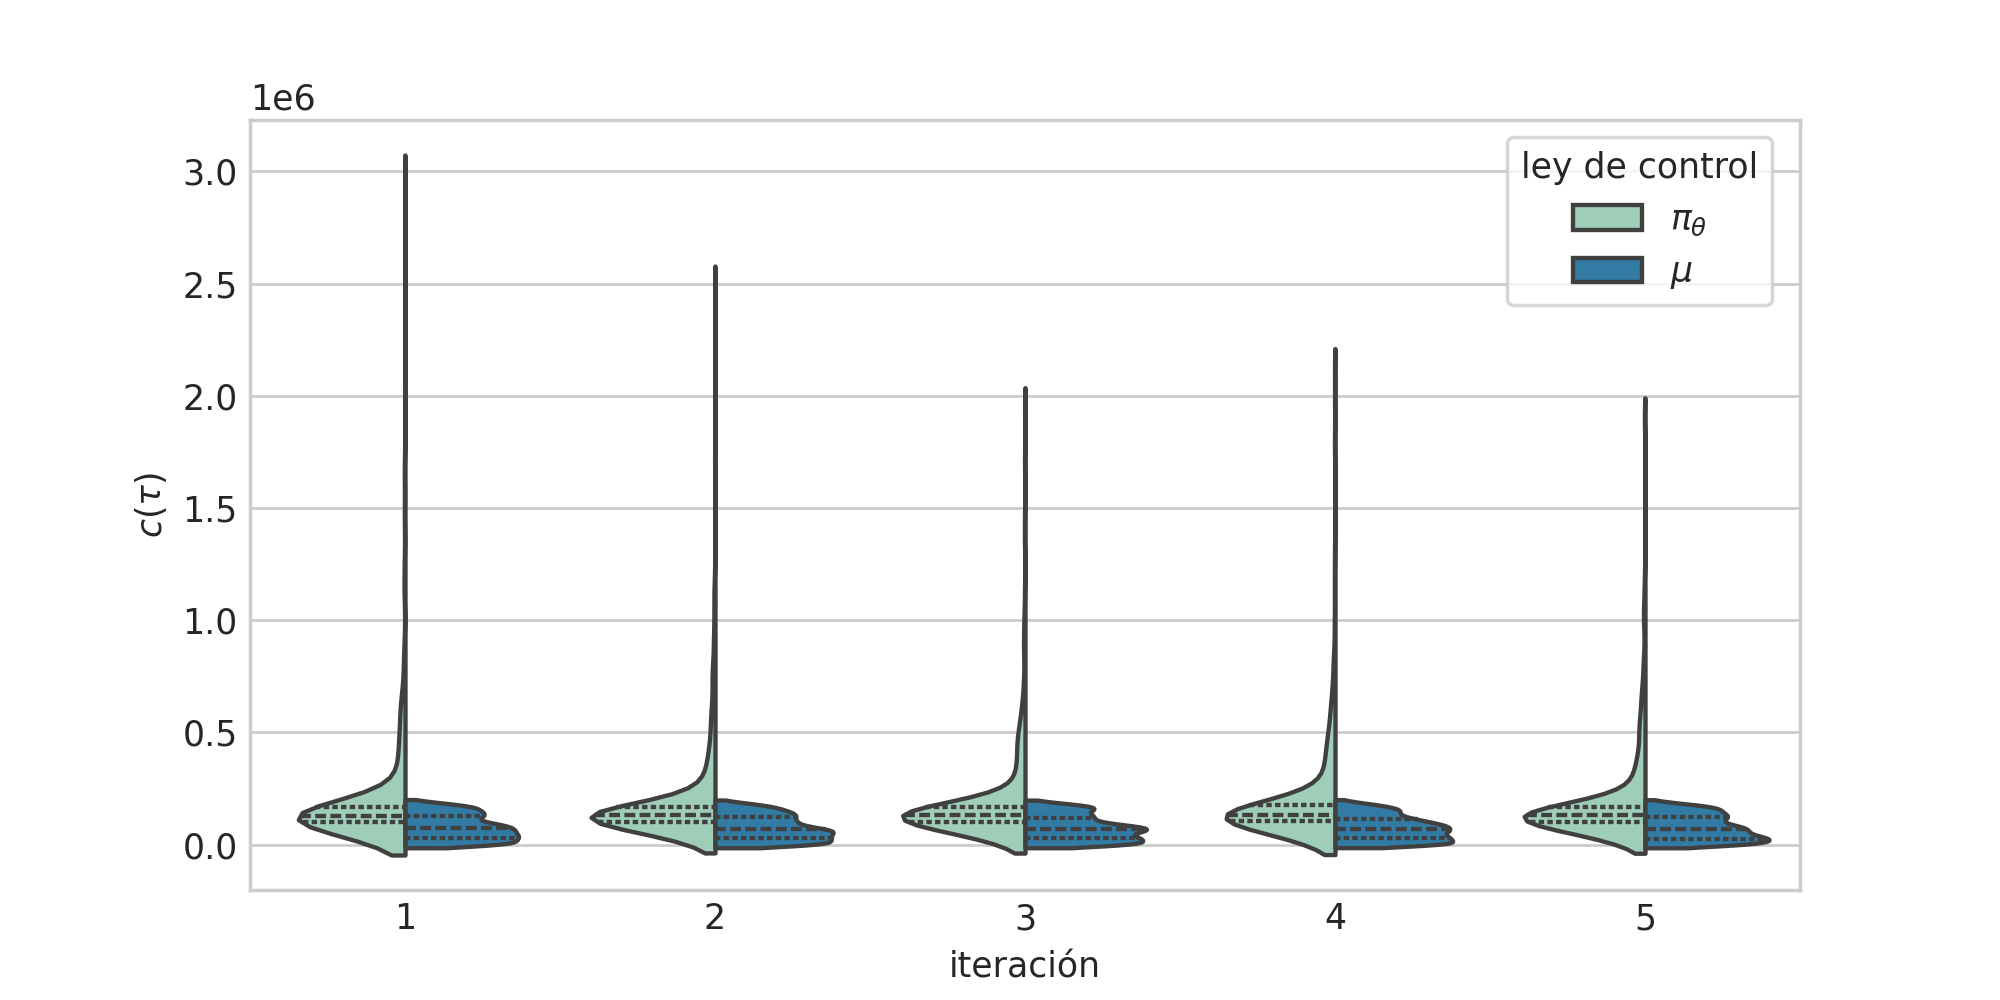
\includegraphics[width=1.0\linewidth]{06_aplicacion_y_evaluacion_de_metodos_rl/policy_vs_control_cost.png}
\caption{Evolución del costo acumulado $c(\bm{\tau})$ de $M=800$ trayectorias usando la ley de control $\mu$ (\acrshort{ilqr}) y la política global (\acrshort{gps}) $\pi_{\bm{\theta}}$ después de cada iteración de entrenamiento.}
\label{fig:gps_cost_evolution}
\end{figure}

\begin{table}[h!]
\centering
\begin{tabular}{|c|c|c|c|}
\hline
\multirow{2}{*}{Iteración} & \multicolumn{3}{c|}{Percentil de $c(\bm{\tau})$} \\ \cline{2-4}
                          & $25 \%$ & $50 \%$ & $75\%$ \\ \hline
1. & $1.22 \times 10^5$ & $1.35 \times 10^5$ & $1.48 \times 10^5$ \\ 
2. & $1.60 \times 10^5$ & $2.33 \times 10^5$ & $4.07 \times 10^5$ \\ 
3. & $8.35 \times 10^4$ & $1.09 \times 10^5$ & $1.25 \times 10^5$ \\ 
4. & $9.38 \times 10^4$ & $1.21 \times 10^5$ & $1.55 \times 10^5$ \\ 
5. & $5.46 \times 10^4$ & $1.26 \times 10^5$ & $1.63 \times 10^5$ \\ 
\hline
\end{tabular}
\caption{Evolución de los percentiles 25, 50 y 75 de la distribución del  costo $c(\bm\tau)$ de las trayectorias de prueba durante las iteraciones de optimización \acrshort{gps}.}
\label{tab:gps_cost_evolution}
\end{table}

Otra métrica significativa medir la mejora de la política global es la norma del supremo sobre el estado final $\mathbf{x}_T$. En este caso se observa una disminución en la dispersión entre el primer cuartil y tercer cuartil de la distribución, al pasar del $[3.09, 6.54]$ al $[0.71, 2.69]$ como se puede observar en el cuadro \ref{tab:gps_norms_percetiles}.

\begin{table}[h!]
\centering
\begin{tabular}{|c|c|c|c|}
\hline
\multirow{2}{*}{Iteración} & \multicolumn{3}{c|}{Percentil de $\|\mathbf{x}_T\|_{\infty}$} \\ \cline{2-4}
                          & $25 \%$ & $50 \%$ & $75\%$ \\ \hline
1. & $3.09$ & $4.32$ & $6.54$ \\ 
2. & $11.00$ & $35.40$ & $99.40$ \\ 
3. & $1.63 $ & $2.36$ & $2.72$ \\ 
4. & $1.36$ & $2.08$ & $2.84$ \\ 
5. & $0.71$ & $1.47$ & $2.69$ \\ 
\hline
\end{tabular}
\caption{Evolución de los percentiles 25, 50 y 75 de la distribución de la norma del supremo de $\mathbf{x}_{T}$ de las trayectorias de prueba durante las iteraciones de optimización \acrshort{gps}.}
\label{tab:gps_norms_percetiles}
\end{table}

Al hacer un análisis más profundo sobre las muestras de $\mathbf{x}_T$ se puede observar en el cuadro \ref{tab:gps_norms_percetiles} que todas las coordenadas tienen una dispersión muy baja salvo la variable $\psi$ (ver estimación de densidades en \ref{fig:gps_coordinates_density}). El primer y tercer cuartil de las muestras en $\psi$ son $[-1.3, 1.19]$, lo cual contrasta con los valores para $\theta$ y $\varphi$ que son $[-0.003, 0.007]$ y $[-0.004, 0.004]$, respectivamente.

\begin{figure}[h!]
\centering
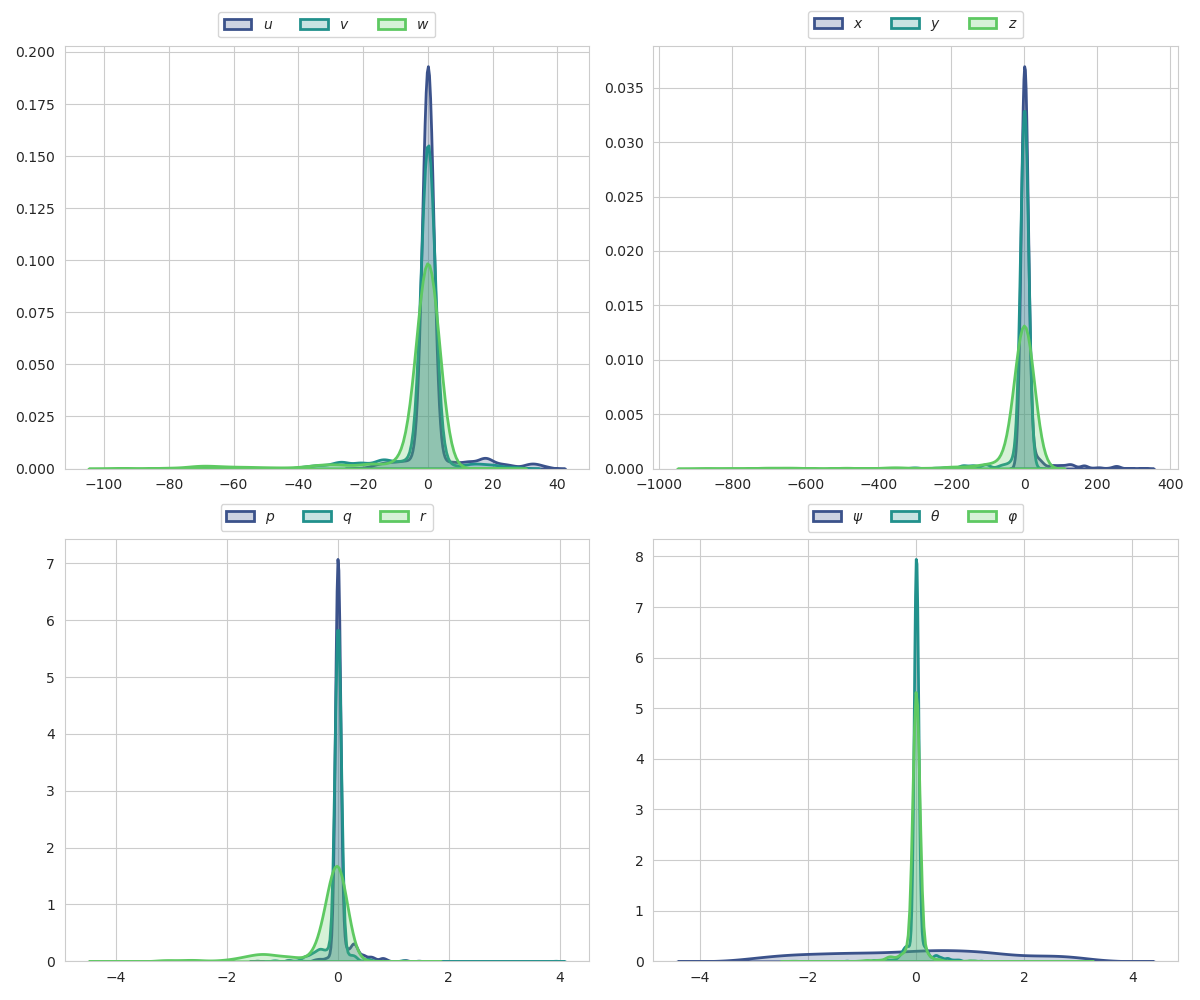
\includegraphics[width=0.8\linewidth]{06_aplicacion_y_evaluacion_de_metodos_rl/gps_coordinates_density.png}
\caption{Densidad de variables de estado al tiempo final $T=30$}
\label{fig:gps_coordinates_density}
\end{figure}



\begin{table}[H]
\centering
\begin{tabular}{|c|r|r|r|}
\hline
\textbf{Variable} & \textbf{25\%} & \textbf{50\%} & \textbf{75\%} \\ \hline
$u$       & -0.074 & 0.003 & 0.086 \\ \hline
$v$       & -0.121 & -0.025 & 0.036 \\ \hline
$w$       & -0.226 & -0.001 & 0.100 \\ \hline
$x$       & 0.042  & 0.094 & 0.232 \\ \hline
$y$       & -0.010 & 0.091 & 0.153 \\ \hline
$z$       & -0.217 & 0.015 & 0.161 \\ \hline
$p$       & -0.005 & 0.000 & 0.007 \\ \hline
$q$       & -0.008 & 0.000 & 0.004 \\ \hline
$r$       & -0.203 & -0.042 & 0.037 \\ \hline
$\psi$    & -\textbf{1.300} & \textbf{0.077} & \textbf{1.190} \\ \hline
$\theta$  & -0.003 & 0.001 & 0.007 \\ \hline
$\varphi$ & -0.004 & 0.000 & 0.004 \\ \hline
\end{tabular}
\caption{Percentiles 25, 50, 75 de las variables de estado al tiempo final $T=30$ segundos.}
\label{tab:percentiles_state_gps}
\end{table}

\begin{figure}[h!]
\centering
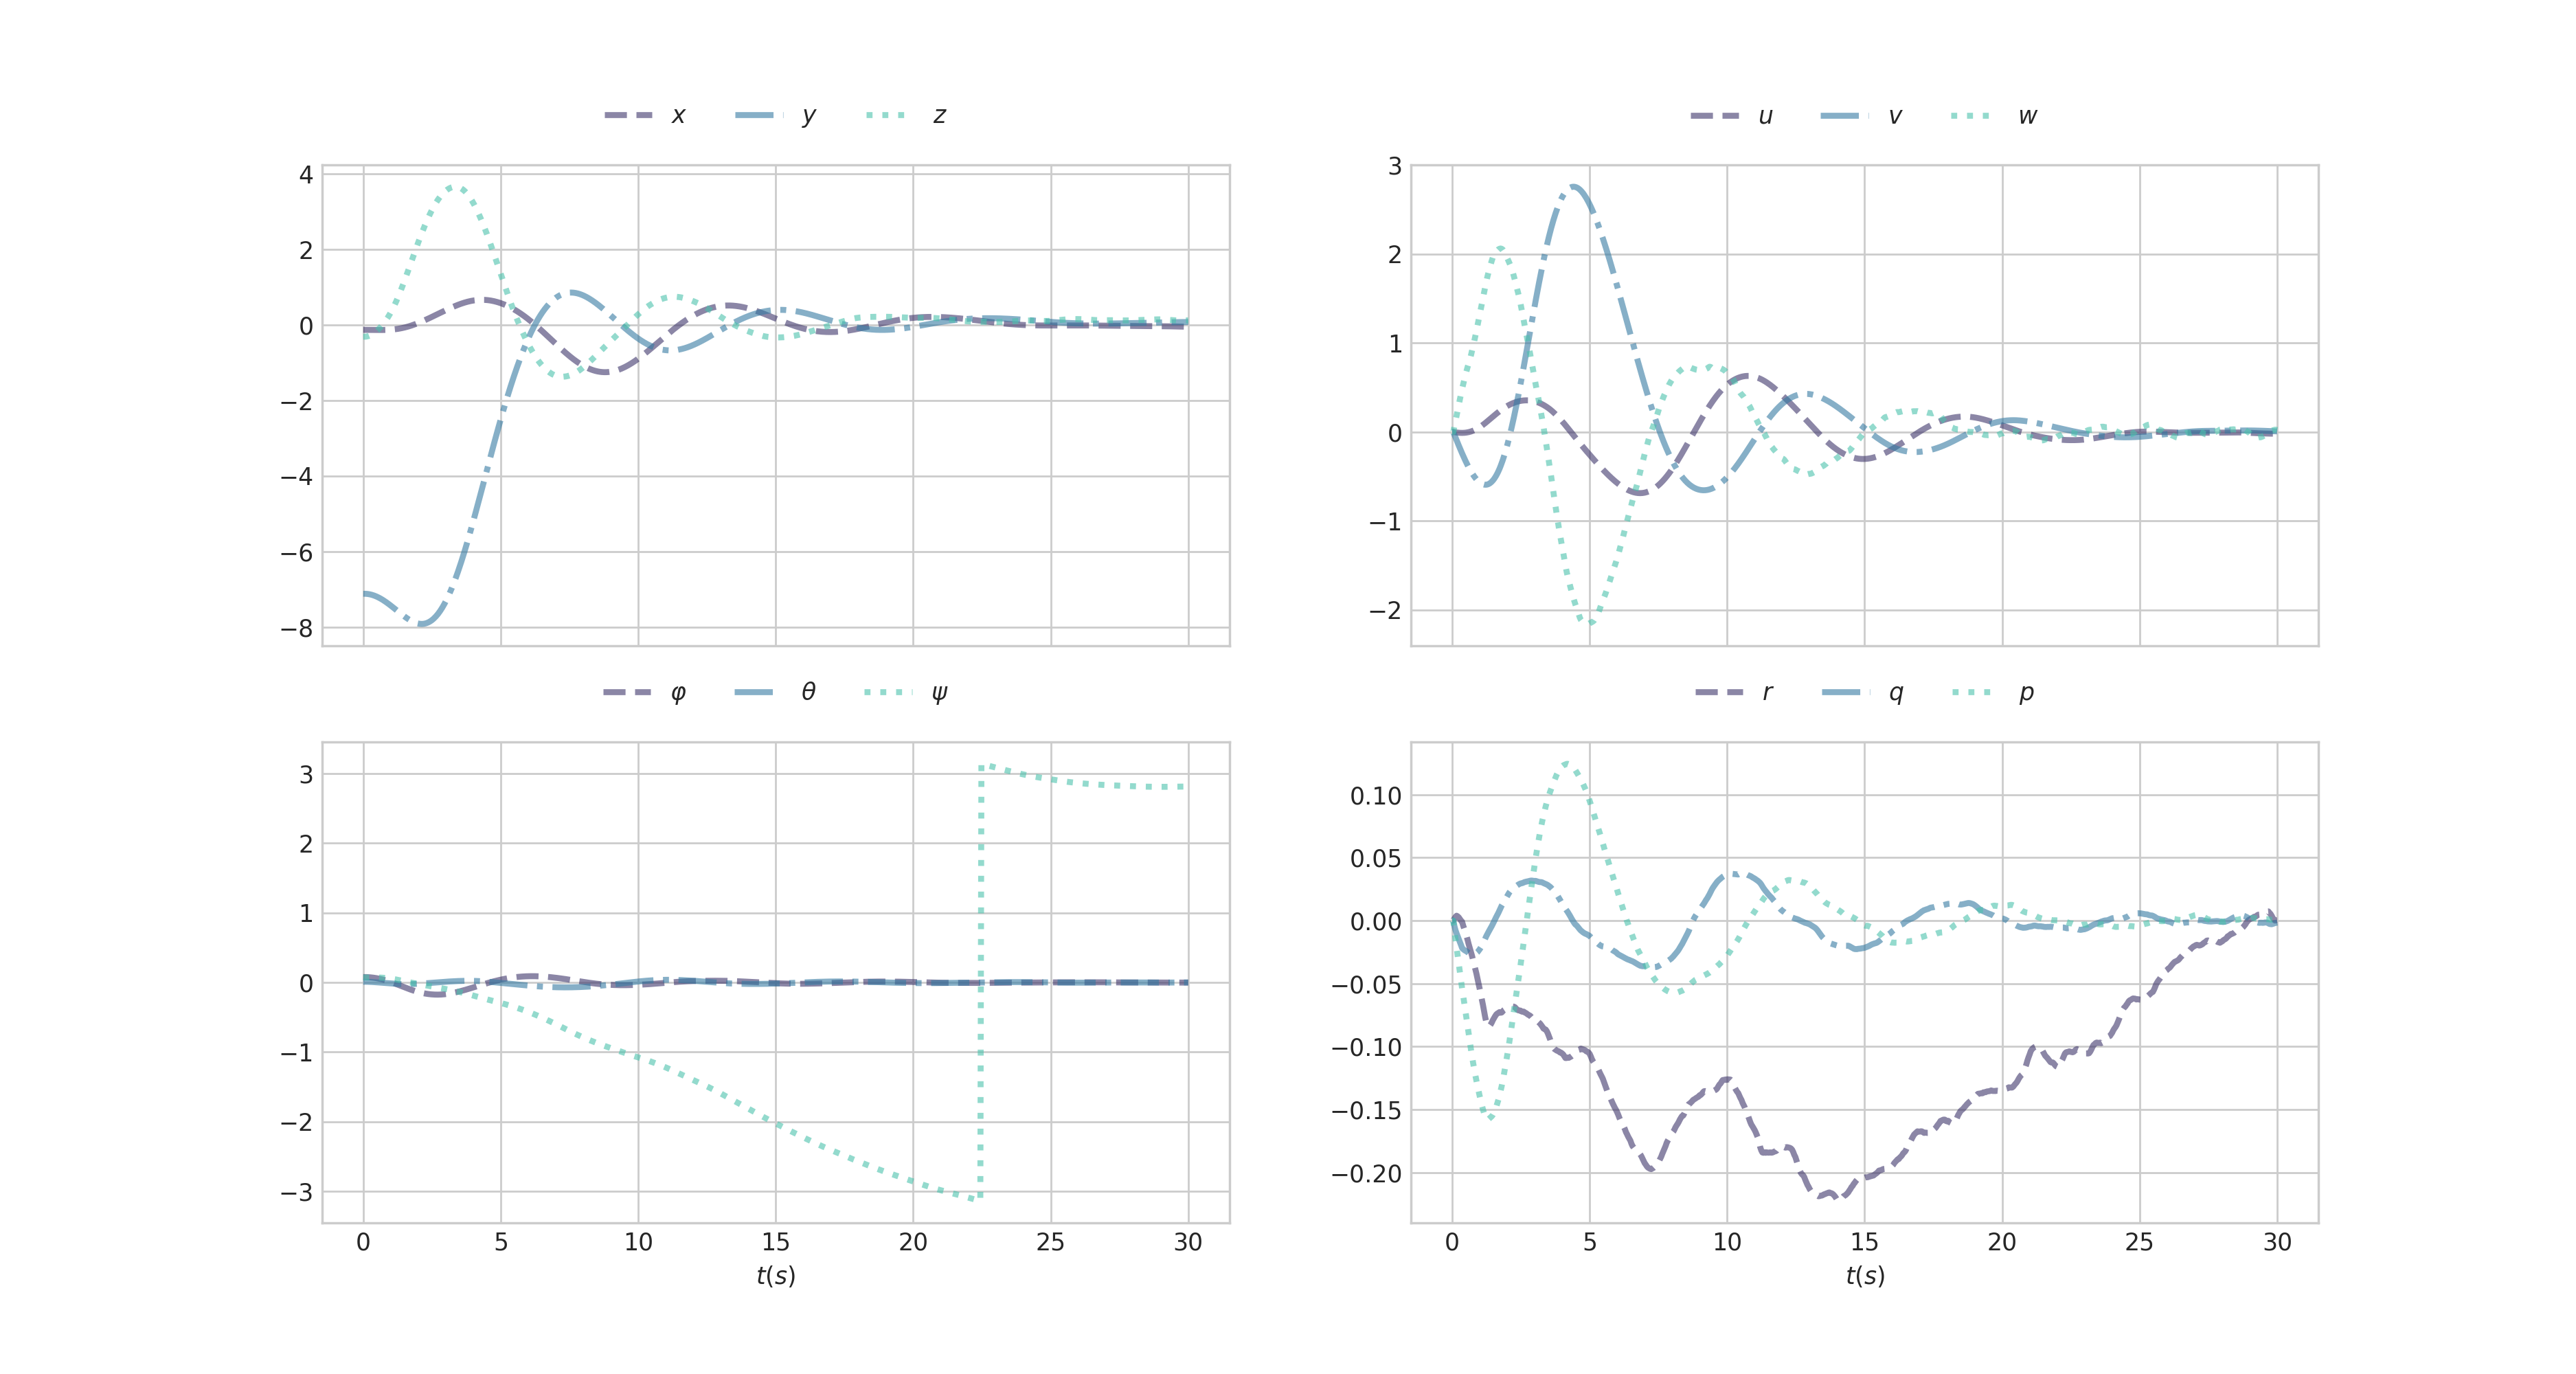
\includegraphics[width=1.0\linewidth]{06_aplicacion_y_evaluacion_de_metodos_rl/gps_states.png}
\caption{Muestra de evolución de coordenadas inerciales $(x, y, z, \phi, \theta, \psi)$ y velocidades locales $(u, v, w, p, q, r)$ bajo la política $\mu_{\bm\theta}$ ajustada con el algoritmo \acrshort{gps} \ref{alg:gps}.}
\label{fig:state_traj_gps}
\end{figure}

\begin{figure}[H]
\centering
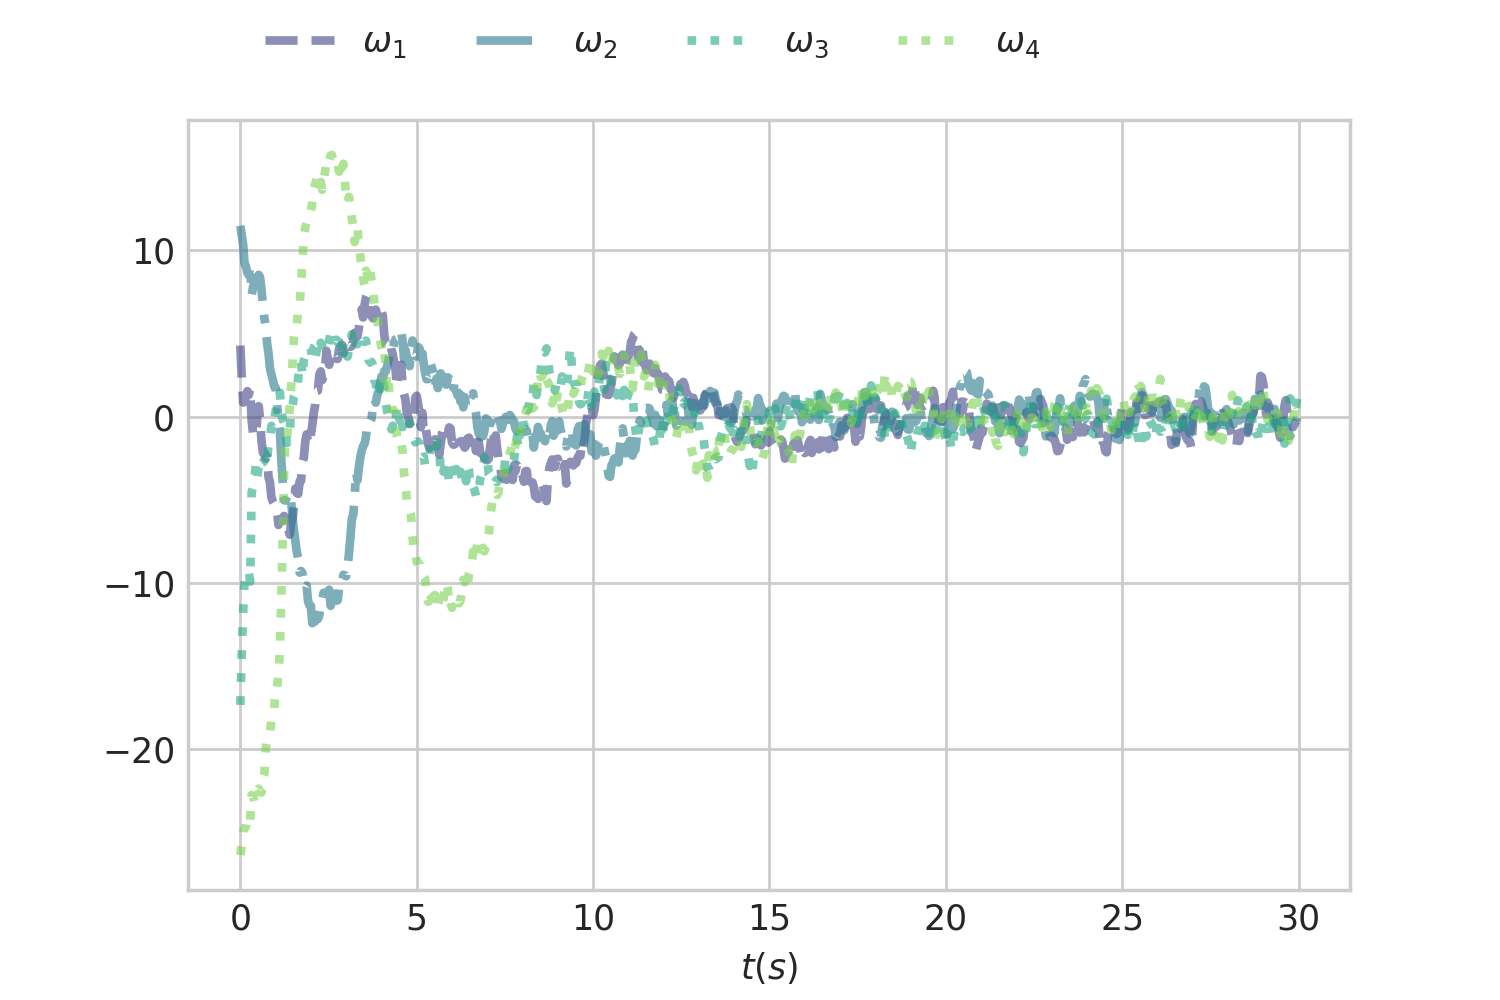
\includegraphics[width=0.6\linewidth]{06_aplicacion_y_evaluacion_de_metodos_rl/gps_actions.png}
\caption{Velocidad de rotores $(\omega_1, \omega_2, \omega_3, \omega_4)$ generadas por la política $\mu_{\bm\theta}$ asociadas a la trayectoria de estado mostrado en la figura \ref{fig:state_traj_gps}.}
\end{figure}

\begin{figure}[H]
\centering
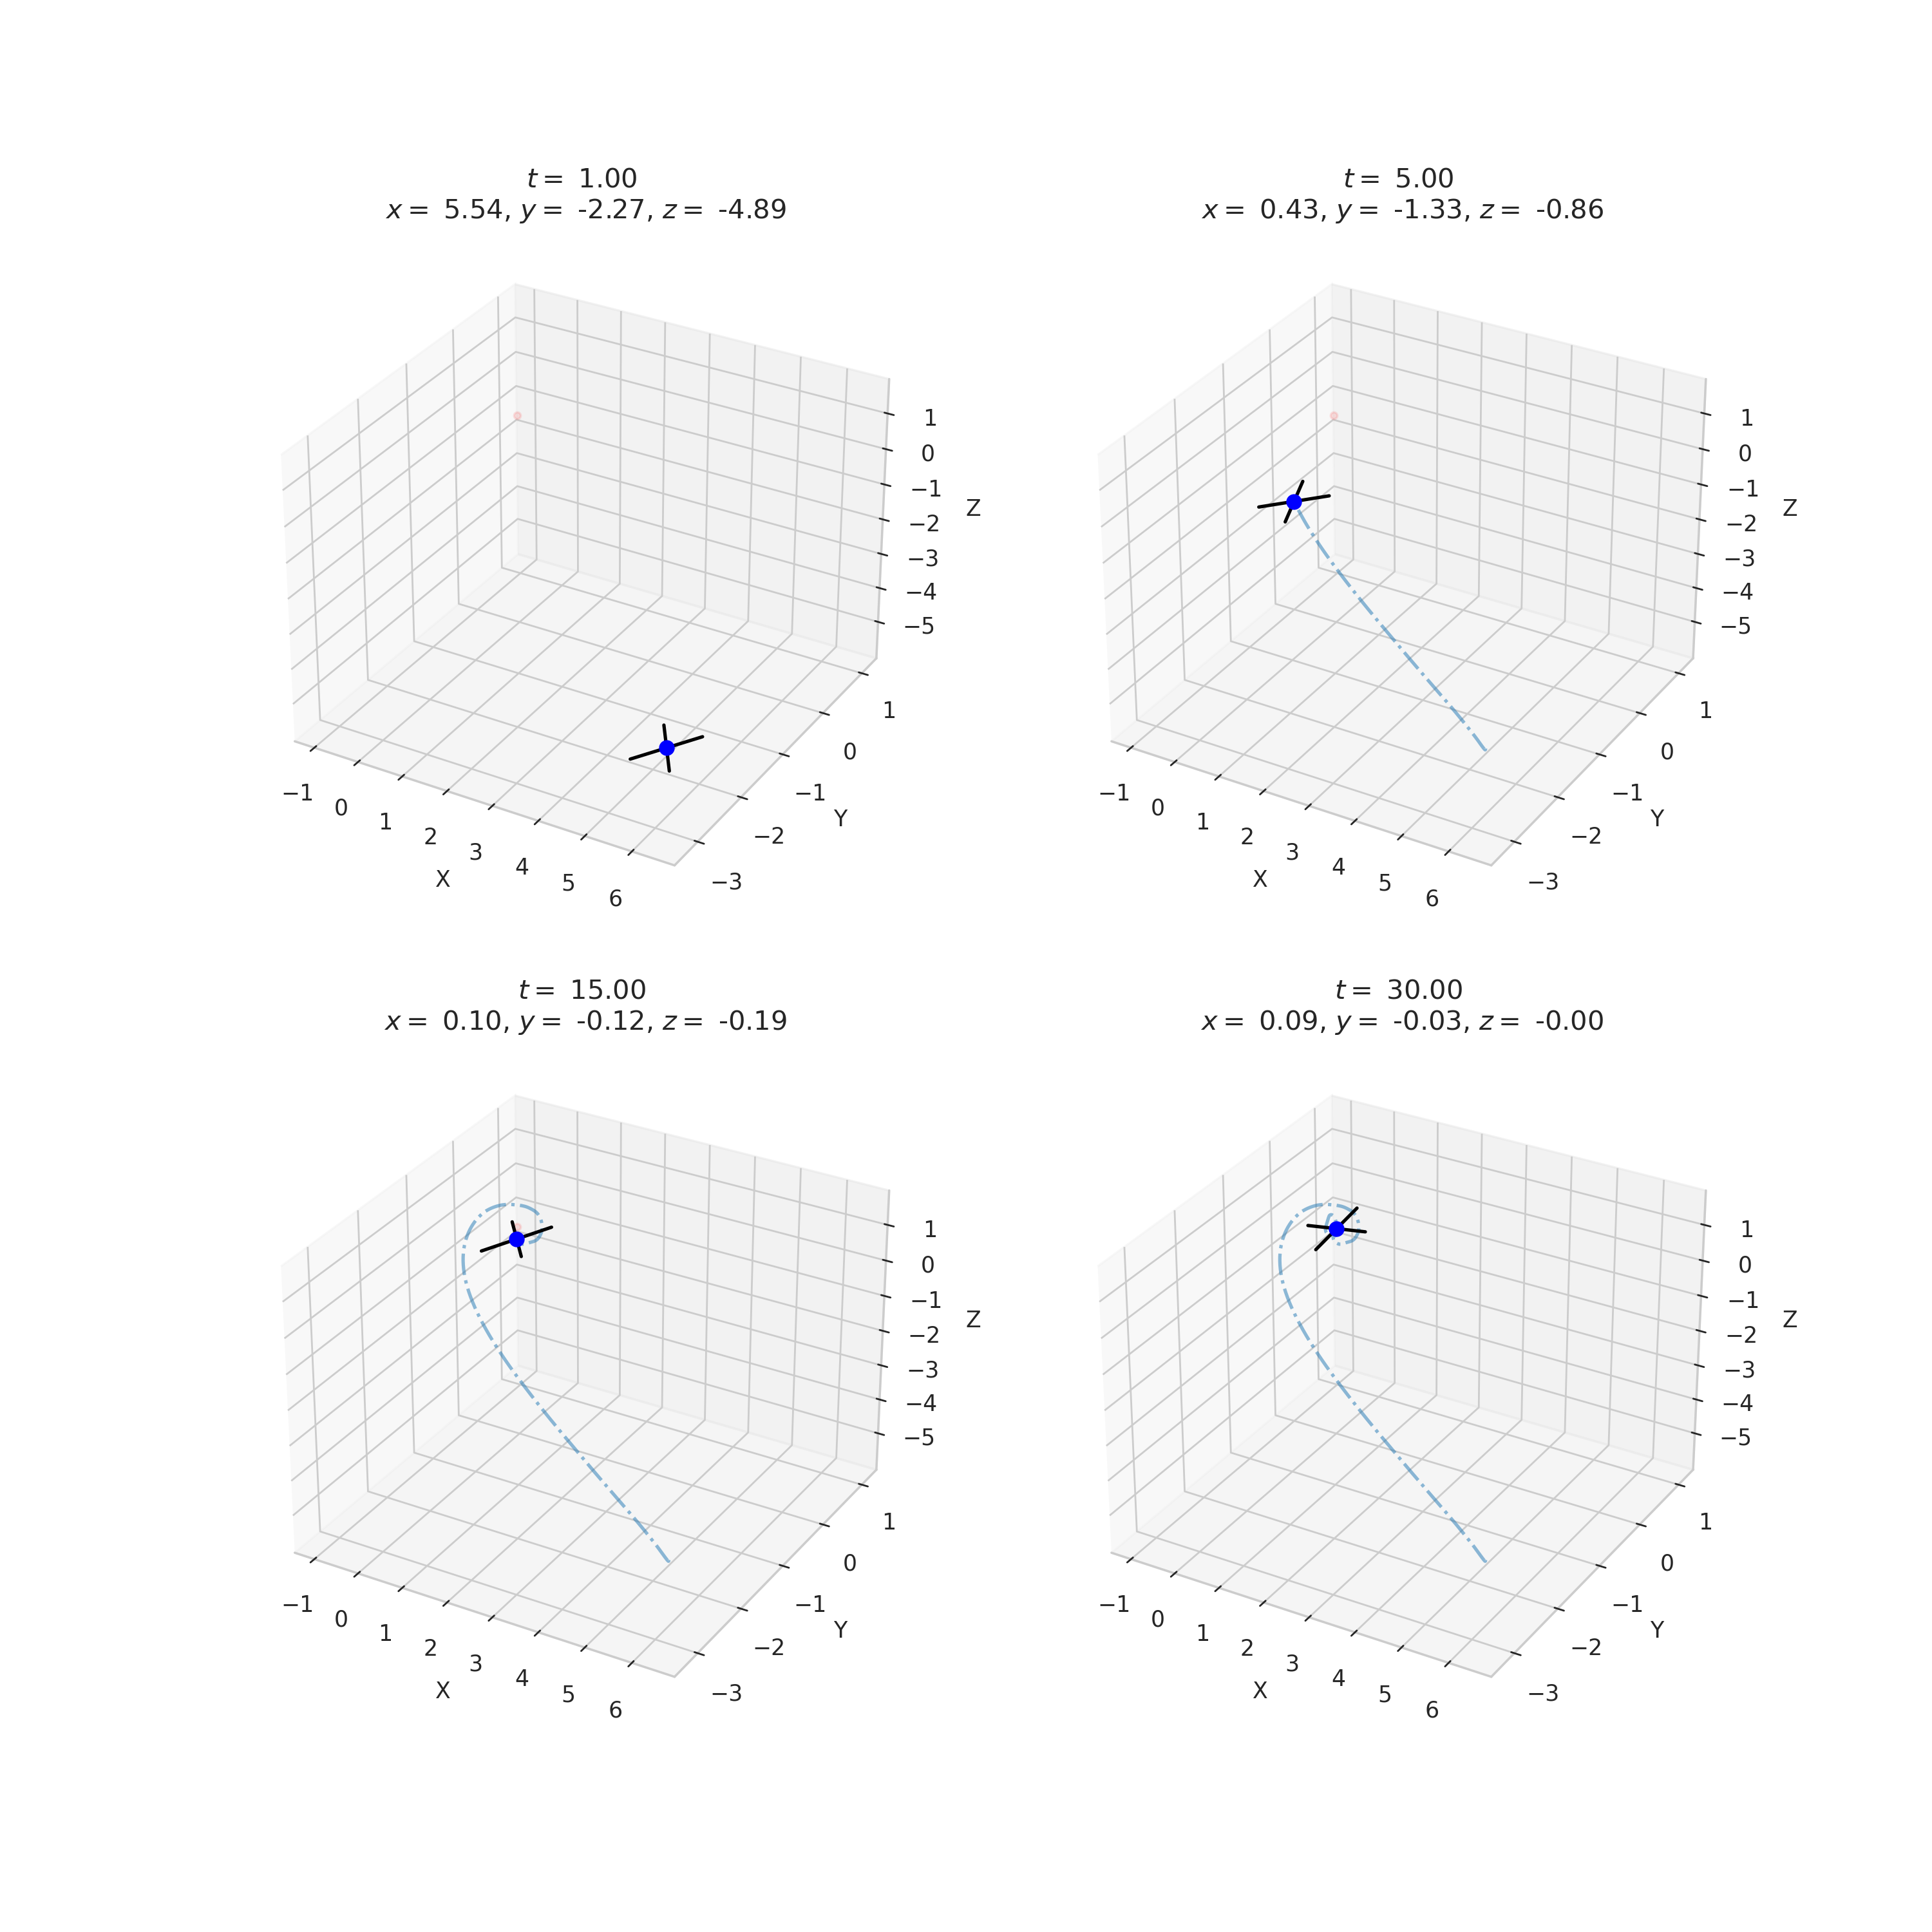
\includegraphics[width=0.8\linewidth]{06_aplicacion_y_evaluacion_de_metodos_rl/animation.png}
\caption{Representación en tres dimensiones de una trayectoria de vuelo en el sistema inercial bajo la política $\mu_{\bm\theta}$ \acrshort{gps} durante los segundos 1, 5, 15 y 30, respectivamente}
\label{fig:gps_results}
\end{figure}

\subsection{Resultados entrenamiento \acrshort{ddpg}}
Para monitorear la optimización de la política durante las 10 \textit{epochs} se recuperaron la estimación de la media y desviación estándar del retorno asociado a los episodios realizados tanto en el entrenamiento como en la validación (ver figura \ref{fig:ddpg_return_evolution}). En ambas gráficas se observa una media muy baja y una desviación estándar muy grande lo cuál indica que no hay convergencia en el aprendizaje.

\begin{figure}[H]
\centering
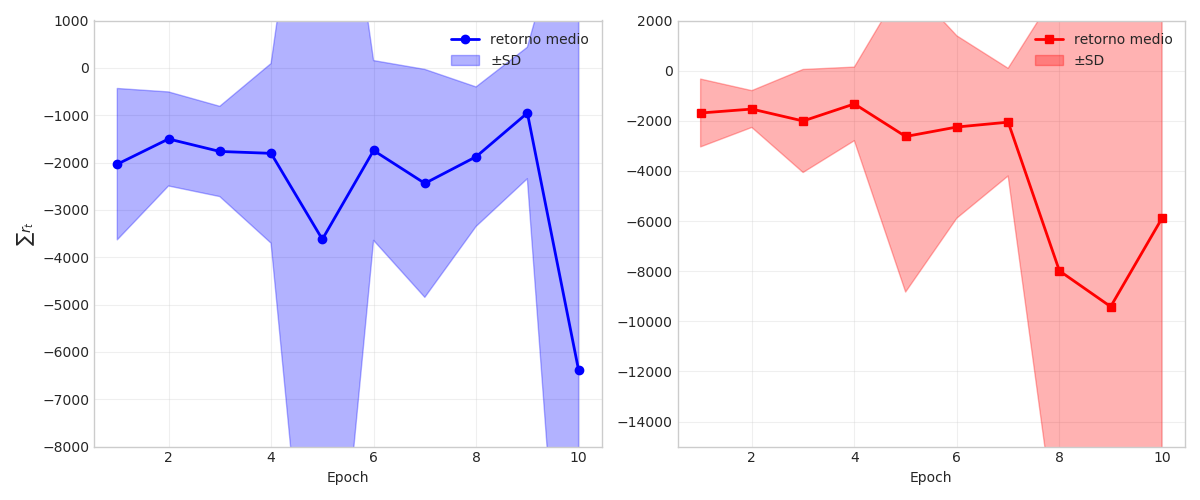
\includegraphics[width=0.8\linewidth]{06_aplicacion_y_evaluacion_de_metodos_rl/ddpg_return_evolution.png}
\caption{Evolución de las estimaciones de la media y la desviación estándar del retorno de los episodios de entrenamiento (azul) y de validación (rojo).}
\label{fig:ddpg_return_evolution}
\end{figure}

Adicionalmente se midió el tamaño promedio de los episodios realizados en el entrenamiento y validación. Se observó en la \textit{epoch} 9 que la política logró terminar todos los episodios en las trayectorias de entrenamiento mientras que en la validación alcanzó a realizar cerca de 600 pasos que equivale a 24 segundos de un máximo de 30. La cantidad de pasos realizados en promedio por \textit{epoch} se puede observar en \ref{tab:epoch_eplen}. Esto indica la política en la \textit{epoch} 9 logró mantenerse cerca del área de interés a pesar de que el retorno recompensas no fue constantemente alto. 

\begin{table}[H]
\centering
\begin{tabular}{|c|c|c|}
\hline
\multirow{2}{*}{\textbf{Epoch}} & \multicolumn{2}{c|}{\textbf{Tamaño de episodio}} \\
\cline{2-3}
 & \textbf{Entrenamiento} & \textbf{Prueba} \\
\hline
1 & 113.0625 & 82.77 \\
\hline
2 & 82.06383 & 67.47 \\
\hline
3 & 72.05882 & 104.56 \\
\hline
4 & 123.29032 & 95.6 \\
\hline
5 & 103.27273 & 141.49 \\
\hline
6 & 152.0 & 101.91 \\
\hline
7 & 113.84375 & 134.34 \\
\hline
8 & 230.92857 & 605.61 \\
\hline
\textbf{9} & \textbf{750.0} & \textbf{599.02} \\
\hline
10 & 313.64285 & 268.87 \\
\hline
\end{tabular}
\caption{\textit{Epoch} vs. Tamaño de episodio promedio}
\label{tab:epoch_eplen}
\end{table}

Se recuperó la política asociada a la \textit{epoch} 9. Al igual que en los resultados del método \acrshort{gps} se realizaron $800$ episodios de prueba y se analizaron sus respectivos estados finales $\mathbf{x}_T$. En el cuadro de percentiles \ref{tab:ddpg_coordinates_dispersion} y en las densidades de la figura \ref{fig:ddpg_coordinates_density} se puede observar que la dispersión de las coordenadas esta considerablemente lejos del origen salvo por las variables $u, v, p, q, \theta$ y $\psi$.

\begin{figure}[H]
\centering
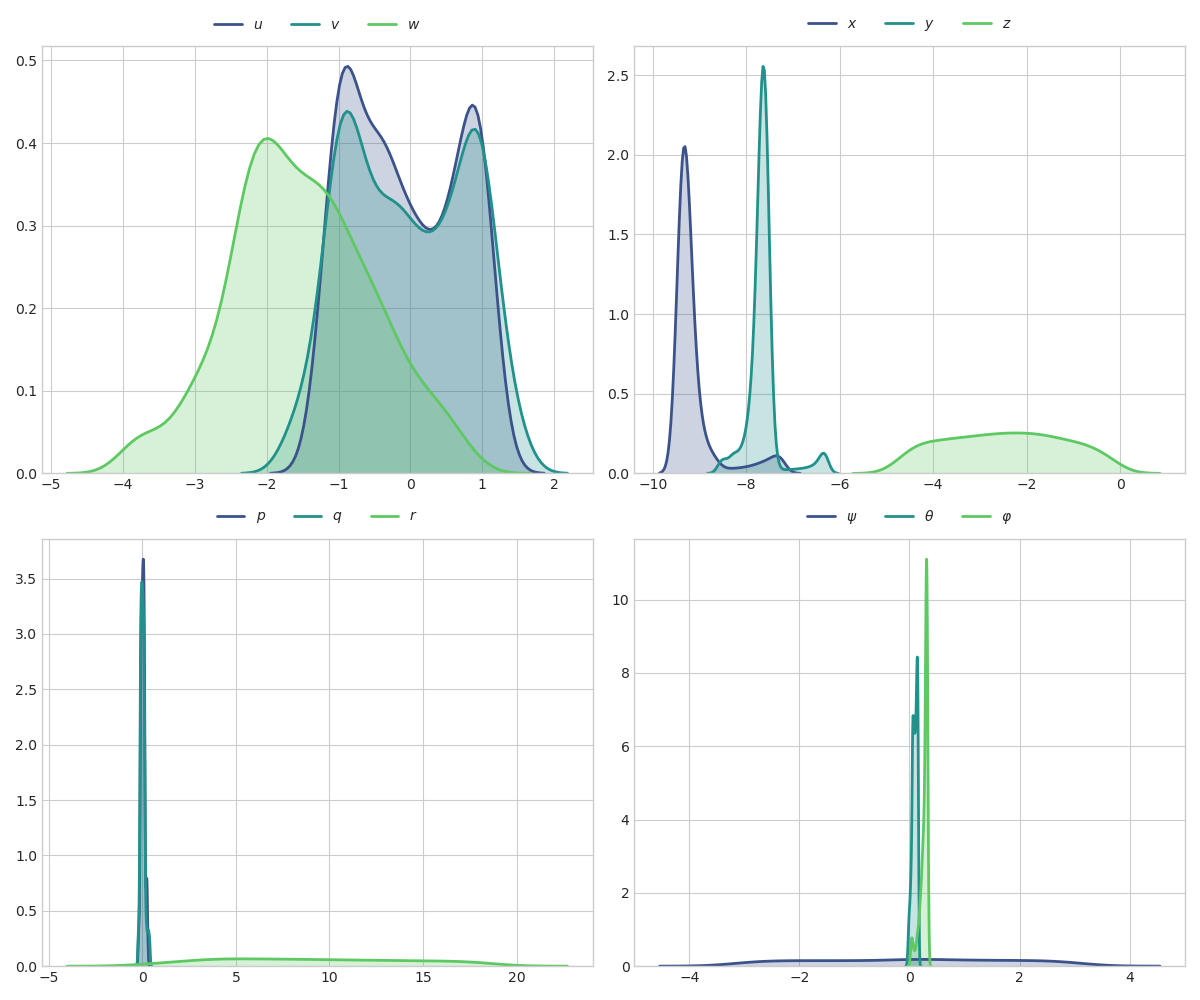
\includegraphics[width=0.8\linewidth]{06_aplicacion_y_evaluacion_de_metodos_rl/ddpg_coordinates_density.png}
\caption{Densidad de variables de estado al tiempo final $T=30$.}
\label{fig:ddpg_coordinates_density}
\end{figure}


\begin{table}[H]
\centering
\begin{tabular}{|c|r|r|r|}
\hline
\textbf{Variable} & \textbf{25\%} & \textbf{50\%} & \textbf{75\%} \\ \hline
$u$       & -0.771 & -0.158 & 0.653 \\ \hline
$v$       & -0.811 & -0.081 & 0.749 \\ \hline
$w$       & \textbf{-2.198} & \textbf{-1.562} & \textbf{-0.861} \\ \hline
$x$       & \textbf{-9.372} & \textbf{-9.293} & \textbf{-9.161} \\ \hline
$y$       & \textbf{-7.737} & \textbf{-7.649} & \textbf{-7.571} \\ \hline
$z$       & \textbf{-3.488} & \textbf{-2.458} & \textbf{-1.489} \\ \hline
$p$       & -0.049 & 0.027 & 0.092 \\ \hline
$q$       & -0.066 & 0.006 & 0.082 \\ \hline
$r$       & \textbf{5.057} & \textbf{8.870} & \textbf{13.300} \\ \hline
$\psi$    & \textbf{-1.477} & \textbf{0.057} & \textbf{1.516} \\ \hline
$\theta$  & 0.062 & 0.100 & 0.137 \\ \hline
$\varphi$ & 0.242 & 0.296 & 0.316 \\ \hline
\end{tabular}
\caption{Percentiles 25, 50, 75 de las variables de estado al tiempo final $T=30$ segundos.}
\label{tab:ddpg_coordinates_dispersion}
\end{table}

Adicionalmente se realizó un entrenamiento con $200$ \textit{epochs} en lugar de $10$–el resto de parámetros se preservaron–. No se observó una reducción en la desviación estándar ni mejora en el retorno medio. Además al realizar simulaciones de vuelo se observa que las acciones de la política de entrenamiento extendido, prácticamente, las acciones se volvieron constantes en contraste con aquellas de la política entrenada con 10 \textit{epochs} como se puede observar en la figura \ref{fig:ddpg_actions}. 

\begin{figure*}[h!]
    \centering
    \subfloat[Trayectoria de acciones después de \\9 \textit{epochs}.]{%
        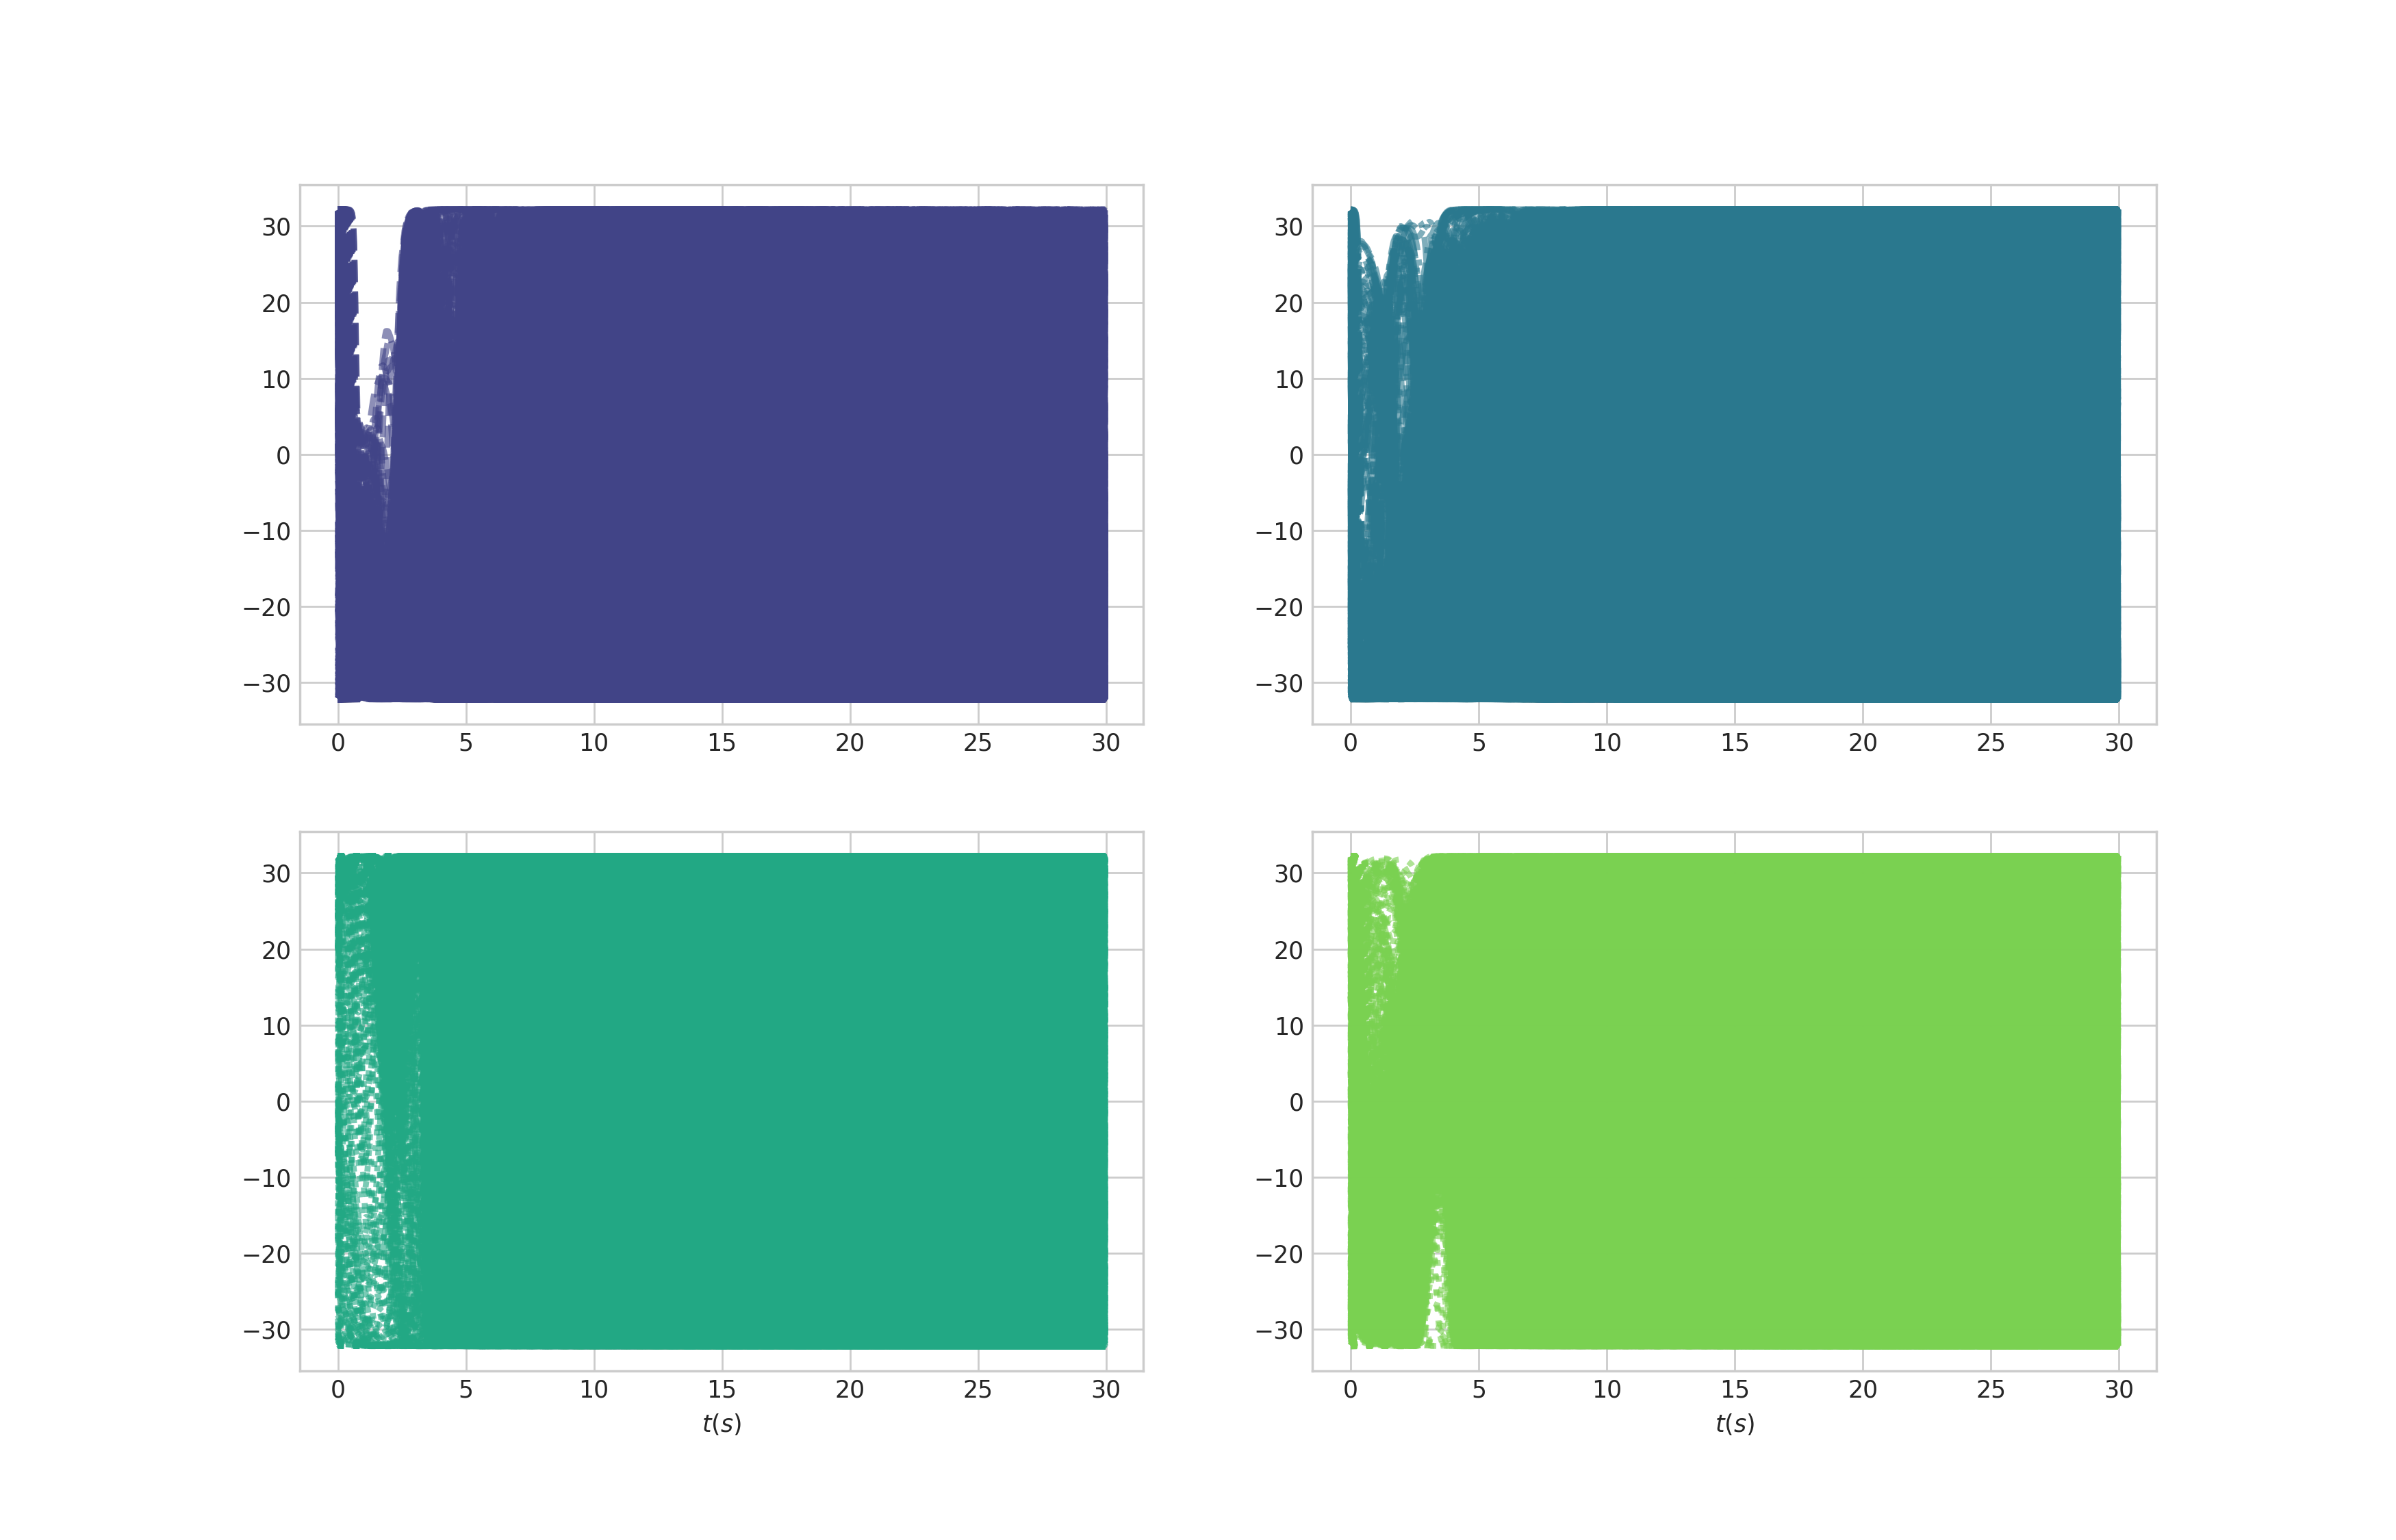
\includegraphics[width=.55\linewidth]{06_aplicacion_y_evaluacion_de_metodos_rl/actions_0.png}%
        \label{subfig:actions_0}
    }
    \subfloat[Trayectoria de acciones después de \\200 \textit{epochs}.]{%
        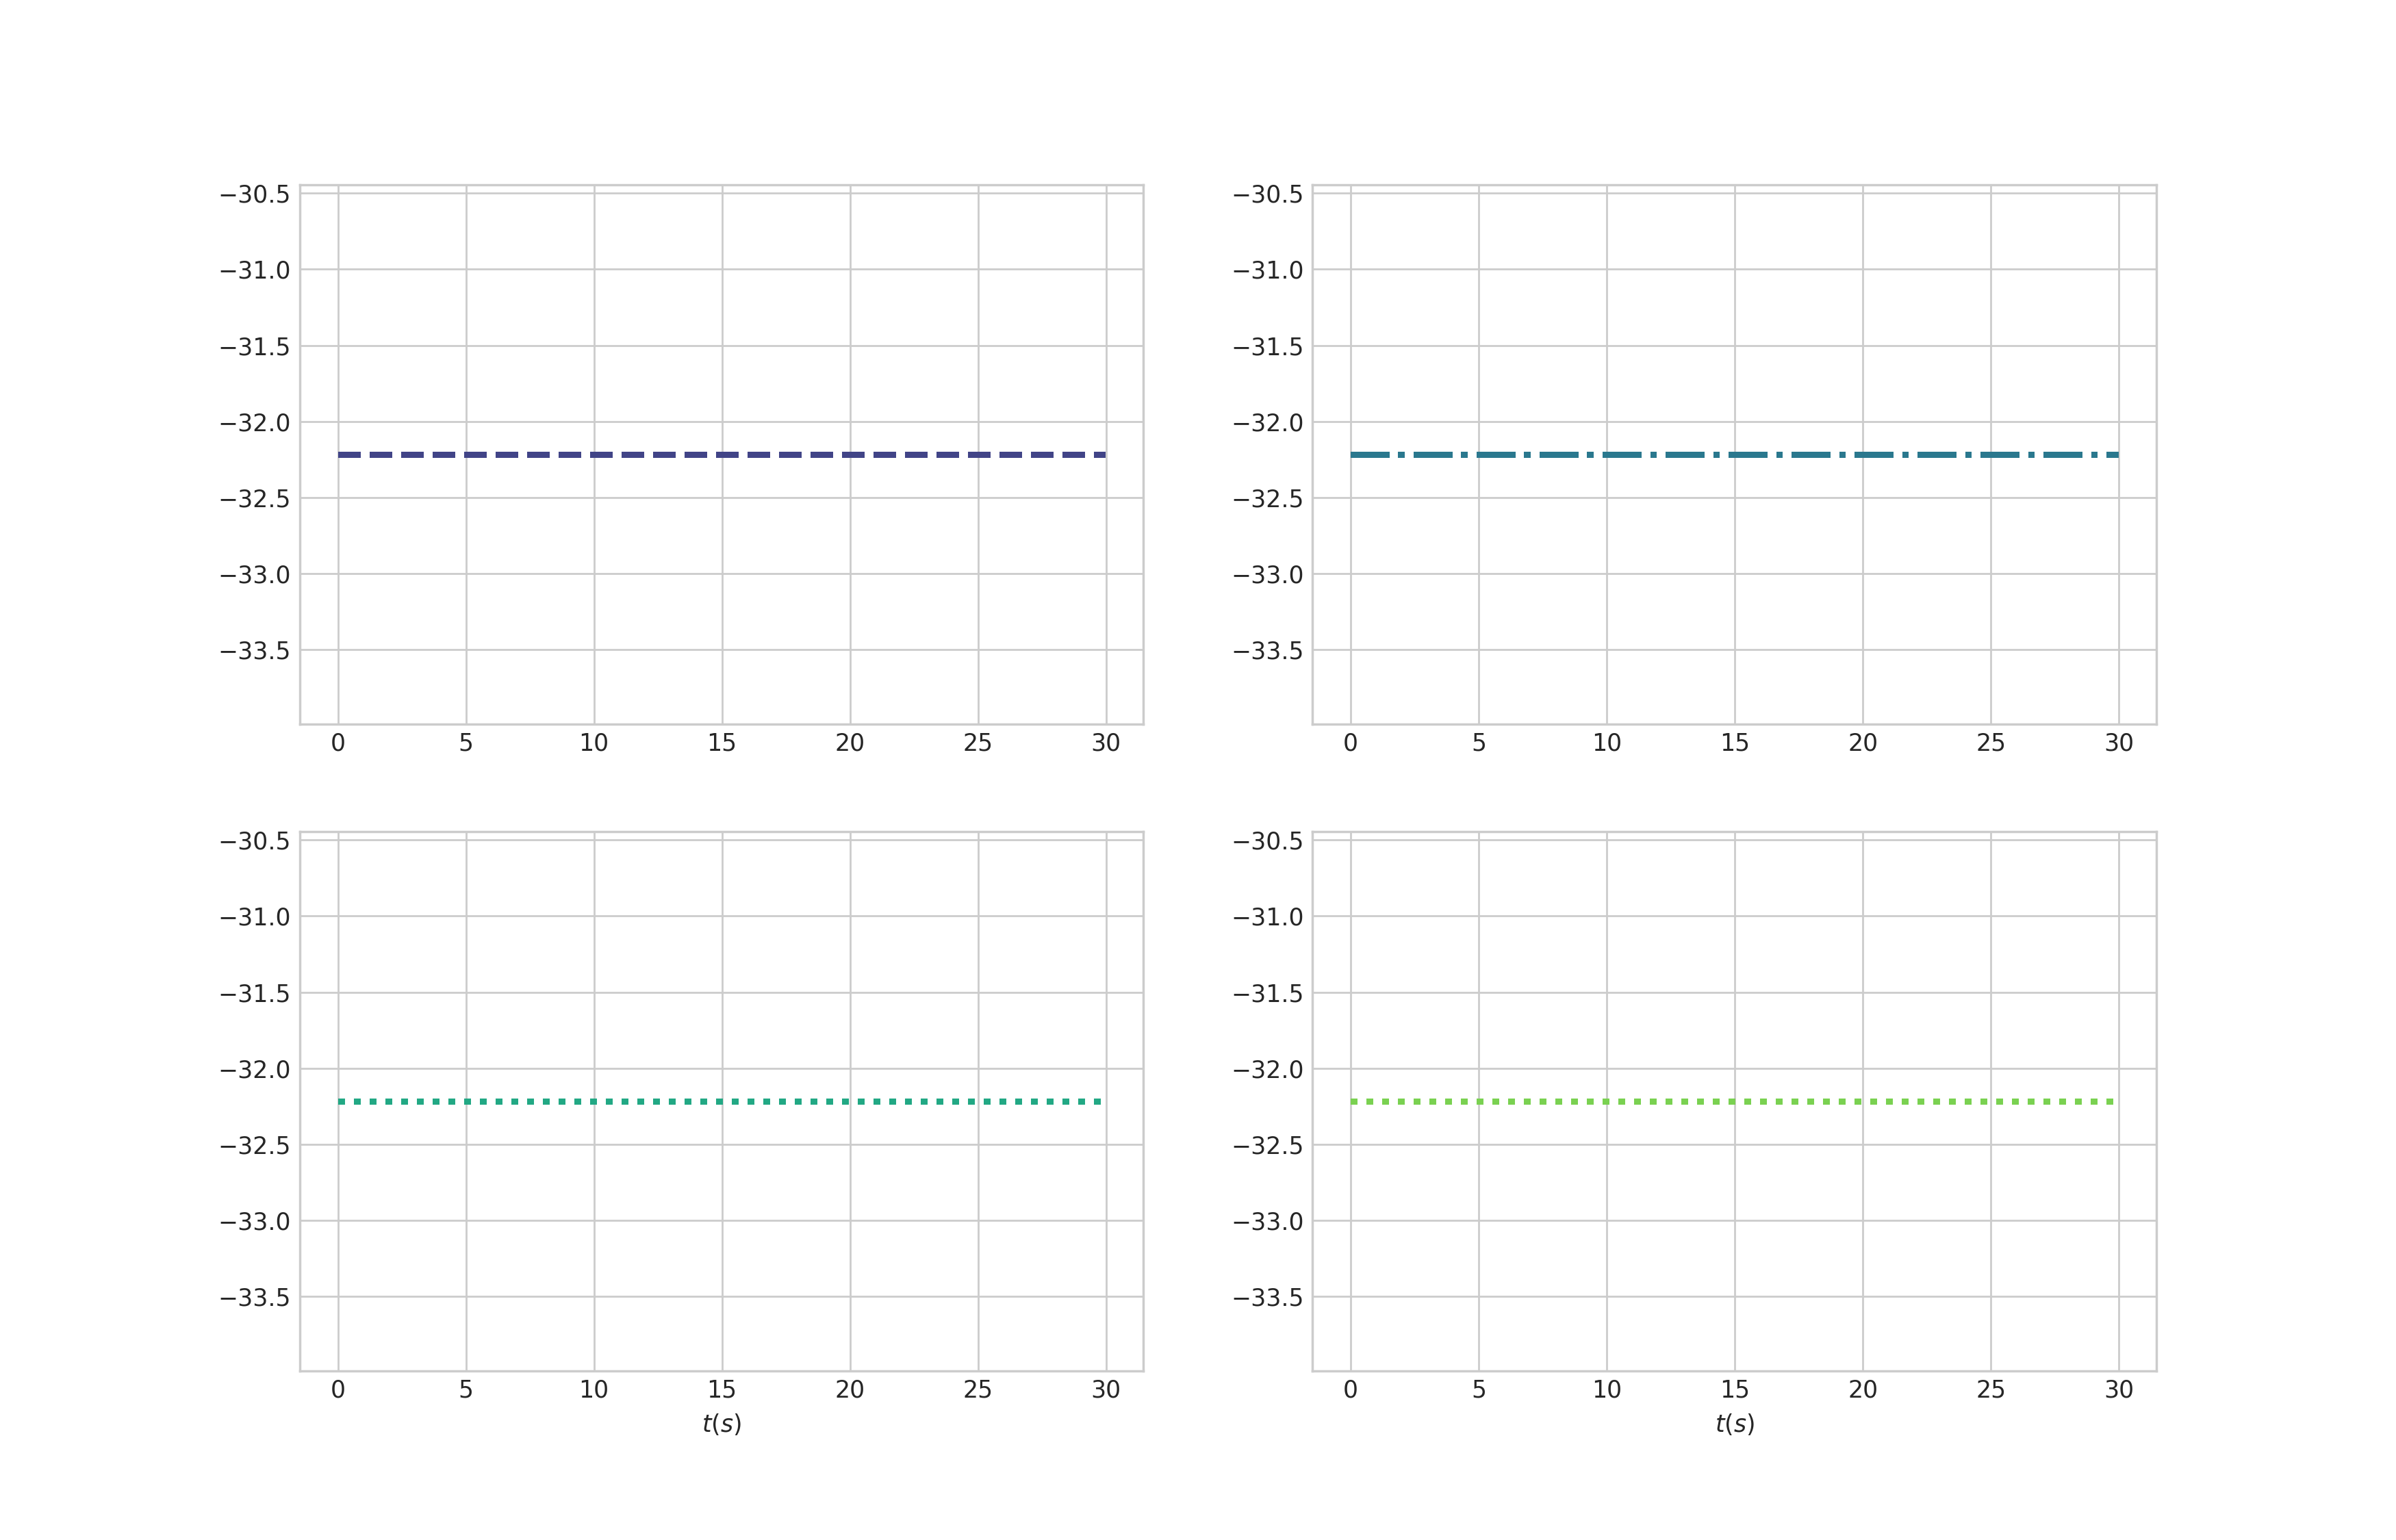
\includegraphics[width=.55\linewidth]{06_aplicacion_y_evaluacion_de_metodos_rl/actions_1.png}%
        \label{subfig:actions_1}
    }
    \caption{Trayectoria de acciones $\omega_1$, $\omega_2$, $\omega_3$ y $\omega_4$ realizadas durante simulaciones con política entrenada después de 10 y 200  \textit{epochs}.}
    \label{fig:ddpg_actions}
\end{figure*}



\subsection{Análisis de estabilidad}
El análisis de estabilidad de sistemas de control es crucial para determinar la confiabilidad del método o la ley del control en distintos escenarios \cite{Busoniu2018}. Retomando lo expuesto en la sección \ref{sec:stability}, informalmente, la estabilidad requiere la contención, esto es que, para unas condiciones iniciales (por ejemplo, dentro de la bola de radio $\delta$ con centro en el origen), el sistema permanece acotado (dentro de la bola de radio $\epsilon$). 

Para analizar la estabilidad del sistema utilizando las diferentes estrategias de control expuestas en este trabajo, se estudió la capacidad del sistema mantenerse en una vecindad cerca del punto de equilibrio a lo largo del tiempo, empezando en un condición inicial distinta a dicho punto. Se consideraron seis conjuntos de condiciones iniciales, $\chi_{ux}$, $\chi_{vy}$, $\chi_{wz}$, $\chi_{p\varphi}$, $\chi_{q\theta}$ y $\chi_{r\psi}$, donde un elemento de cada conjunto representa una condición inicial aleatoria del sistema que vive en un vecindad cerca del origen.   

El conjunto $\chi_{ux}$ se obtiene de seleccionar $N$ posiciones del cuadricoptero, donde los valores $(u, x)$ son muestras aleatorias de dos distribuciones uniformes continuas independientes en con rangos de valores $(x_{-}, x_{+})$ y  $(u_{-}, u_{+})$, respectivamente; el resto de coordenadas son nulas. Formalmente, este conjunto se expresa de la siguiente forma, 
\begin{align}
    \mathcal{X}_{ux} = \left\{[u, 0, 0, x, 0, 0, 0, 0, 0, 0, 0, 0]|\quad u \sim \mathcal{U}(u_{-}, u_{+})\text{, } x \sim \mathcal{U}(x_{-}, x_{+}) \text{: } u_{-} < u_{+}\text{, }x_{-} < x_{+}  \right\}.
\end{align}
Análogamente, se describen los conjuntos $\chi_{vy}$, $\chi_{wz}$, $\chi_{p\varphi}$, $\chi_{q\theta}$ y $\chi_{r\psi}$. Para efectos prácticos $N=10^4$.

\subsubsection{Definición de los criterios de estabilidad}
De acuerdo a la propiedades y resultados recuperados para las distintas estrategias de control en este trabajo, se requiere definir criterios de estabilidad distintos dependiendo del método. Esta diferencia en alcance de cada método implica que estos criterios no son directamente comparables. 

Para analizar la estabilidad de los métodos siempre se verificará si la norma del supremo de coordenadas del estado correspondientes al tiempo final están dentro de una bola abierta de radio $\epsilon$. Lo que distinguirá a los distintos criterios será los grados de libertad considerados. 

\subsubsection{Regiones de estabilidad para feedback linealizado}
Debido a que la capacidad de control de este método sólo recae en la posición $z$ y la orientaciones $\psi, \theta$ y $\varphi$, el criterio de control es, 
    \begin{align}
    \label{eq:lin_creteria}
        \|[w, z, p, q, r, \varphi, \theta, \psi]^{\top}\|_{\infty} < \epsilon \qquad \epsilon > 0.
    \end{align}

Se generaron únicamente trayectorias sobre los conjuntos asociados a las variables relevantes para este controlador: $\mathcal{X}_{wz}, \mathcal{X}_{p\varphi}, \mathcal{X}_{q\theta}$ y $\mathcal{X}_{r\psi}$ Los resultados de este usar este criterio usando $\epsilon=0.5$ sobre los conjuntos se encuentran en el cuadro \ref{tab:stability_region_linear} y la figura \ref{fig:stability_region_linear}. 

\begin{table}[H]
\centering
\begin{tabular}{|c|c|c|c|c|}
\hline
\multirow{2}{*}{Conjunto} & \multirow{2}{*}{Rango} & \% de trayectorias estables \\ 
                          &                          & $t=30$                        \\ \hline
$\chi_{wz}$ & $\pm\text{10.0},\quad\pm\text{20.0}$ & 92.3       \\
$\chi_{p\varphi}$ & $\pm\text{1.0},\quad\pm\pi/2$ & 24.7 \\
$\chi_{q\theta}$ & $\pm\text{1.0},\quad\pm\pi/2$ & 27.6 \\
$\chi_{r\psi}$ & $\pm\text{1.0},\quad\pm\pi/2$ & 97.5 \\
total         & --            & 61.0 \\
\hline
\end{tabular}
\caption{Tasas de trayectorias estables generadas por el controlador ajustado por \textit{feedback} linealizado hasta el segundo $30$ cuya región de estabilidad es mostrada en la figura \ref{fig:stability_region_linear}}
\label{tab:stability_region_linear}
\end{table}

\begin{figure*}[h!]
        \subfloat[Conjunto de condiciones iniciales $\mathcal{X}_{wz}$]{%
            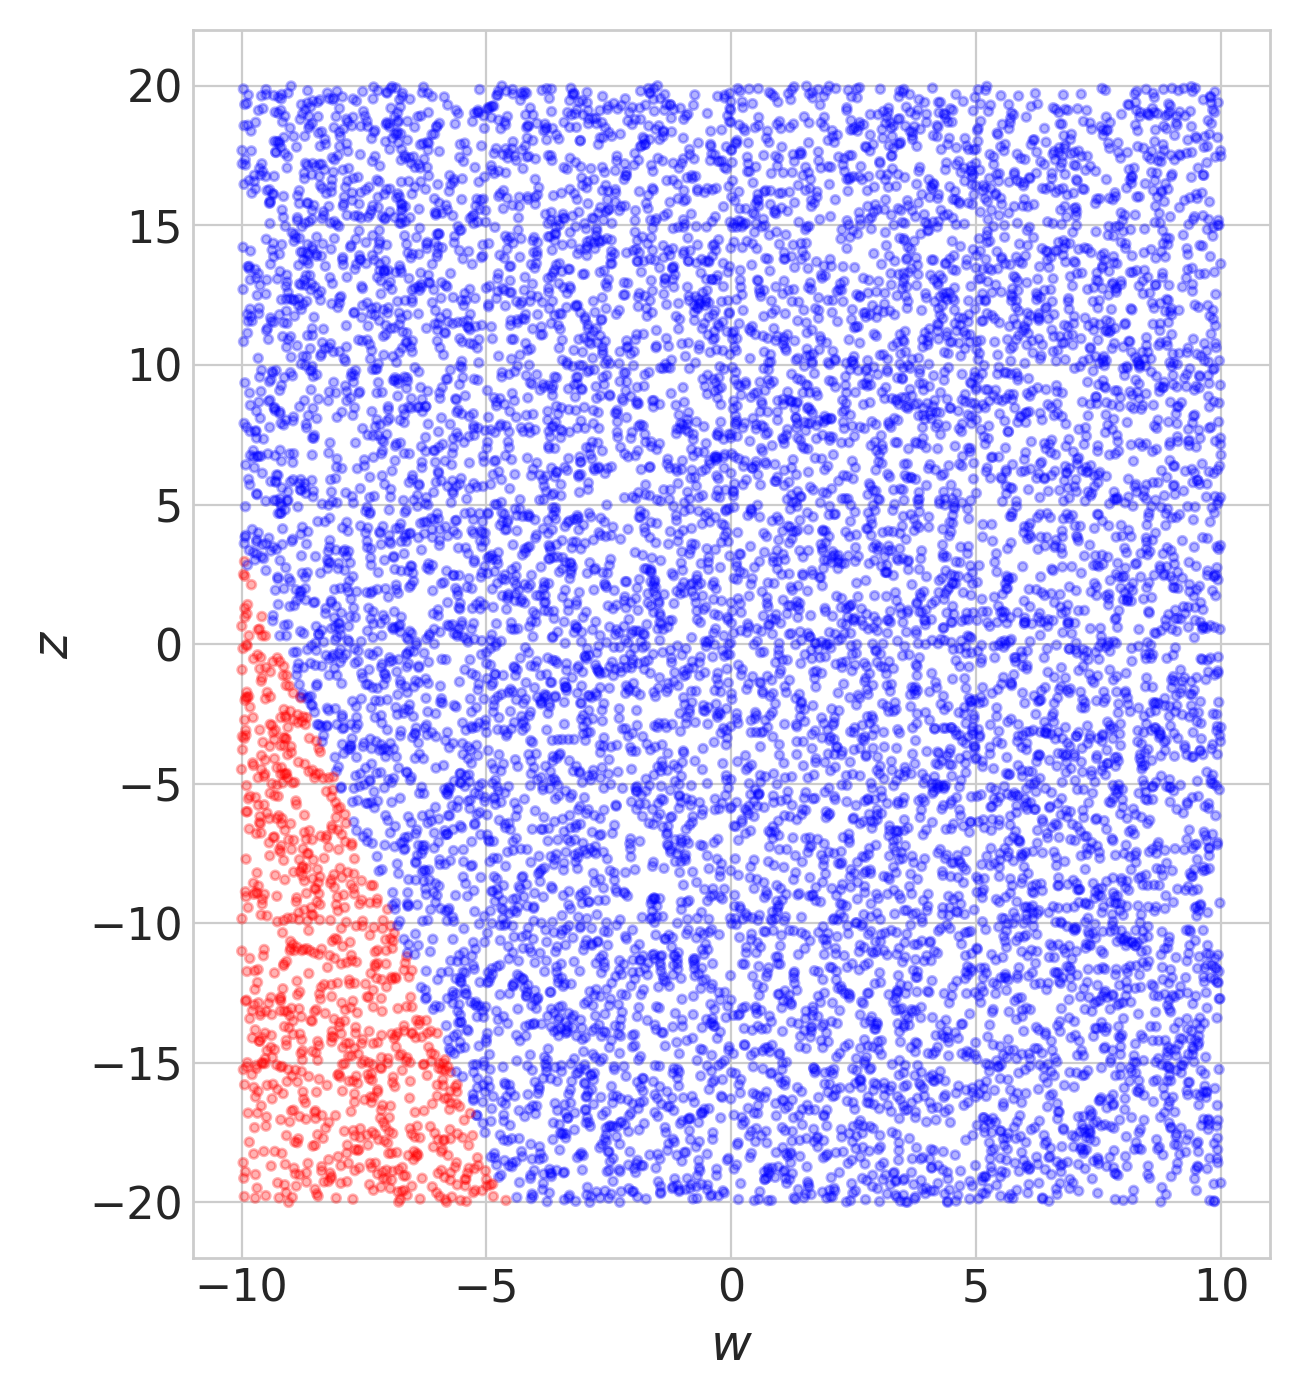
\includegraphics[width=.42\linewidth]{06_aplicacion_y_evaluacion_de_metodos_rl/stability_w-z_th-0_5_t--1_ord-inf_ex-uvxy.png}%
            \label{subfig:z}%
        }
        \subfloat[Conjunto de condiciones iniciales $\mathcal{X}_{p\varphi}$]{%
            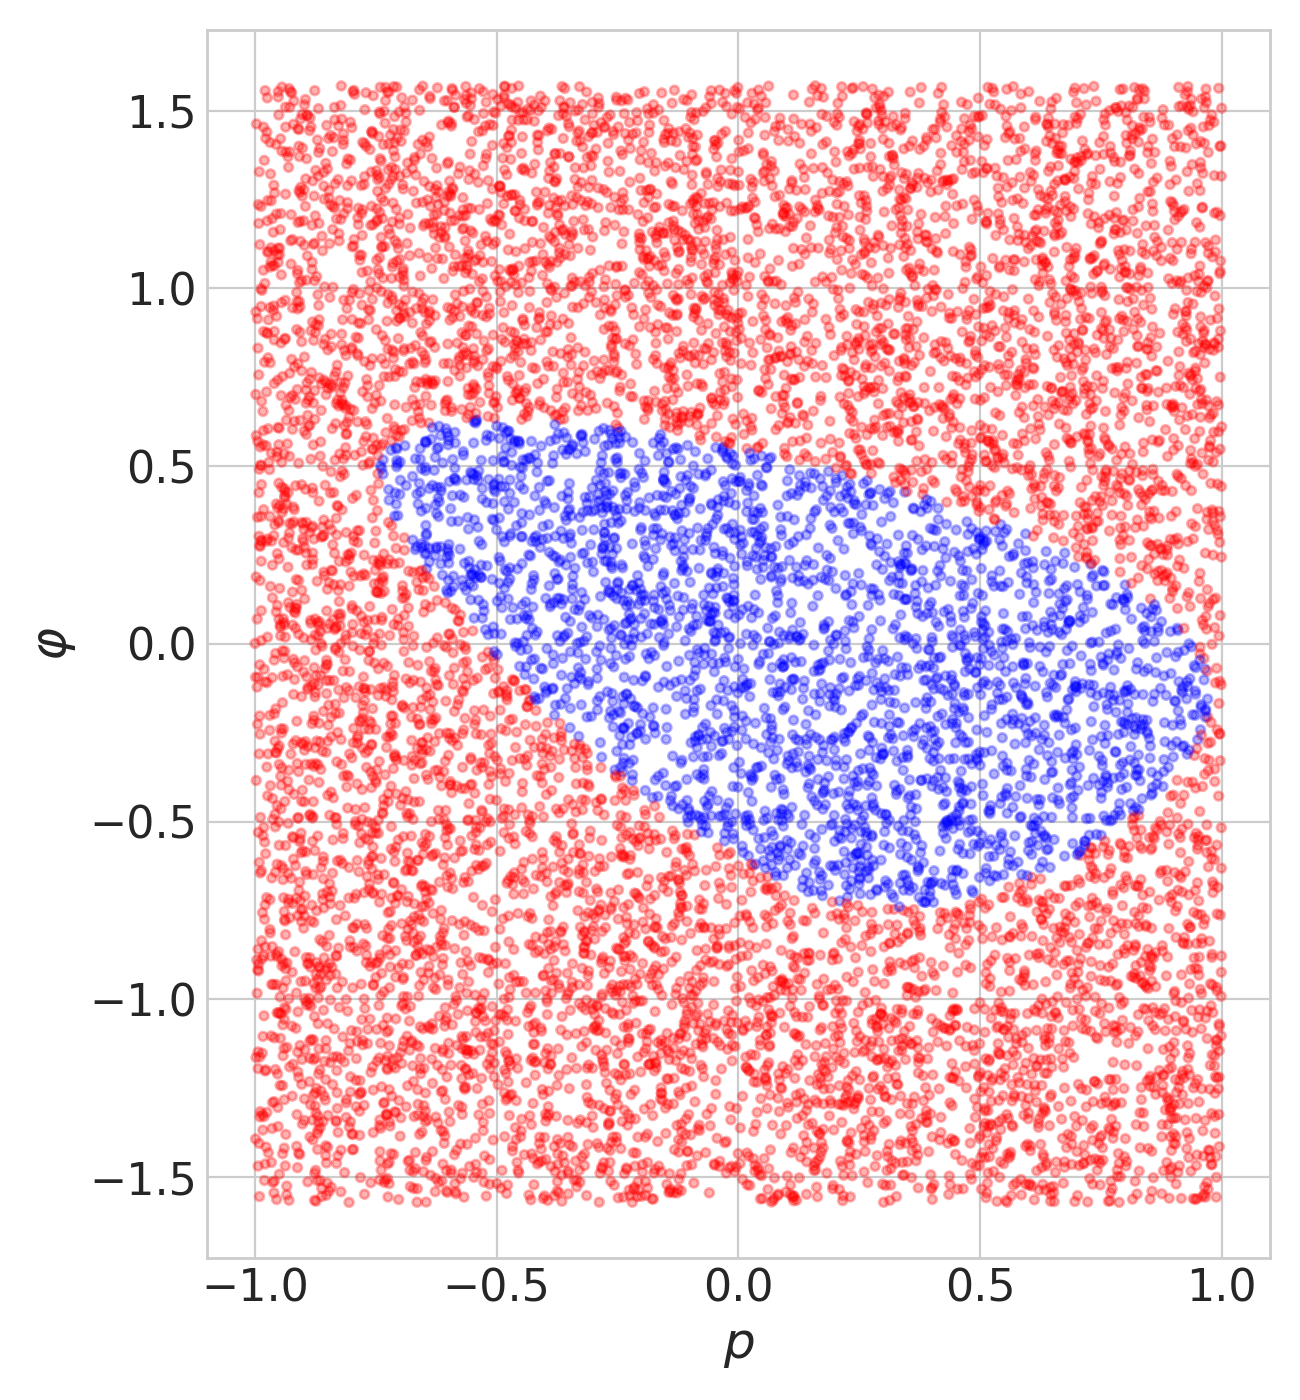
\includegraphics[width=.42\linewidth]{06_aplicacion_y_evaluacion_de_metodos_rl/stability_p-varphi_th-0_5_t--1_ord-inf_ex-uvxy.png}%
            \label{subfig:varphi}%
        }\\
        \subfloat[Conjunto de condiciones iniciales $\mathcal{X}_{q\theta}$]{%
            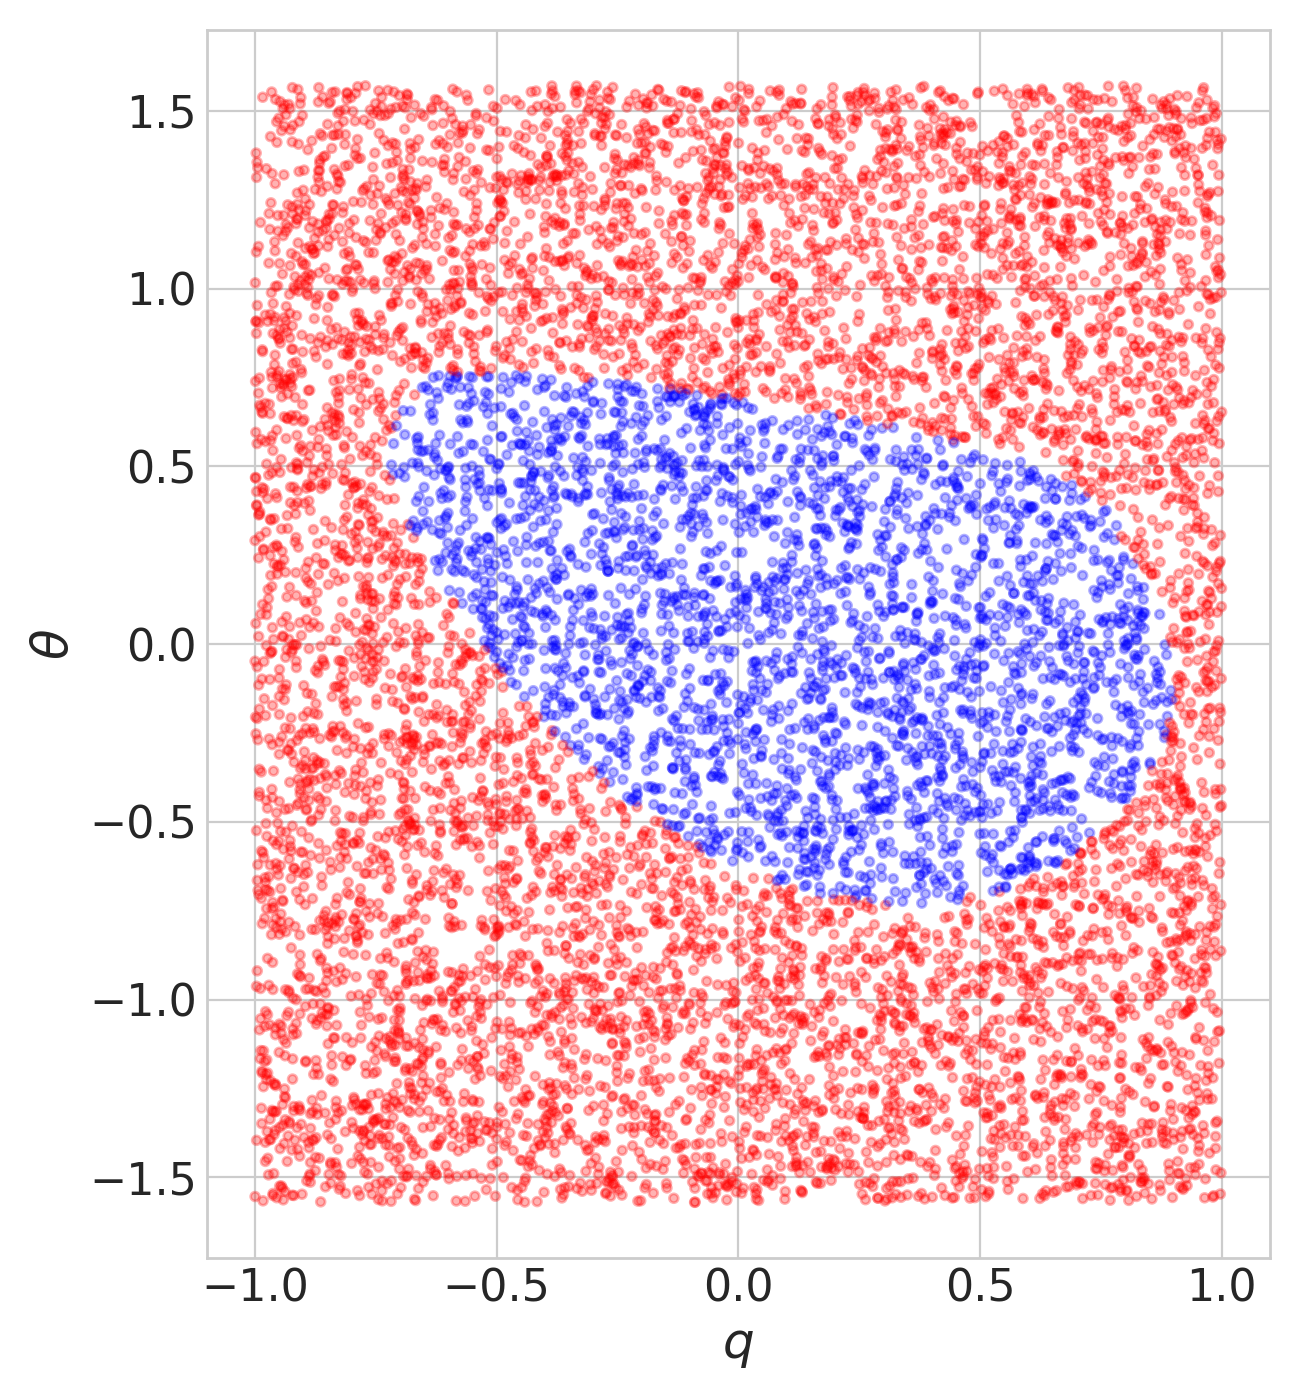
\includegraphics[width=.42\linewidth]{06_aplicacion_y_evaluacion_de_metodos_rl/stability_q-theta_th-0_5_t--1_ord-inf_ex-uvxy.png}%
            \label{subfig:theta}%
        }
        \subfloat[Conjunto de condiciones iniciales $\mathcal{X}_{r\psi}$]{%
            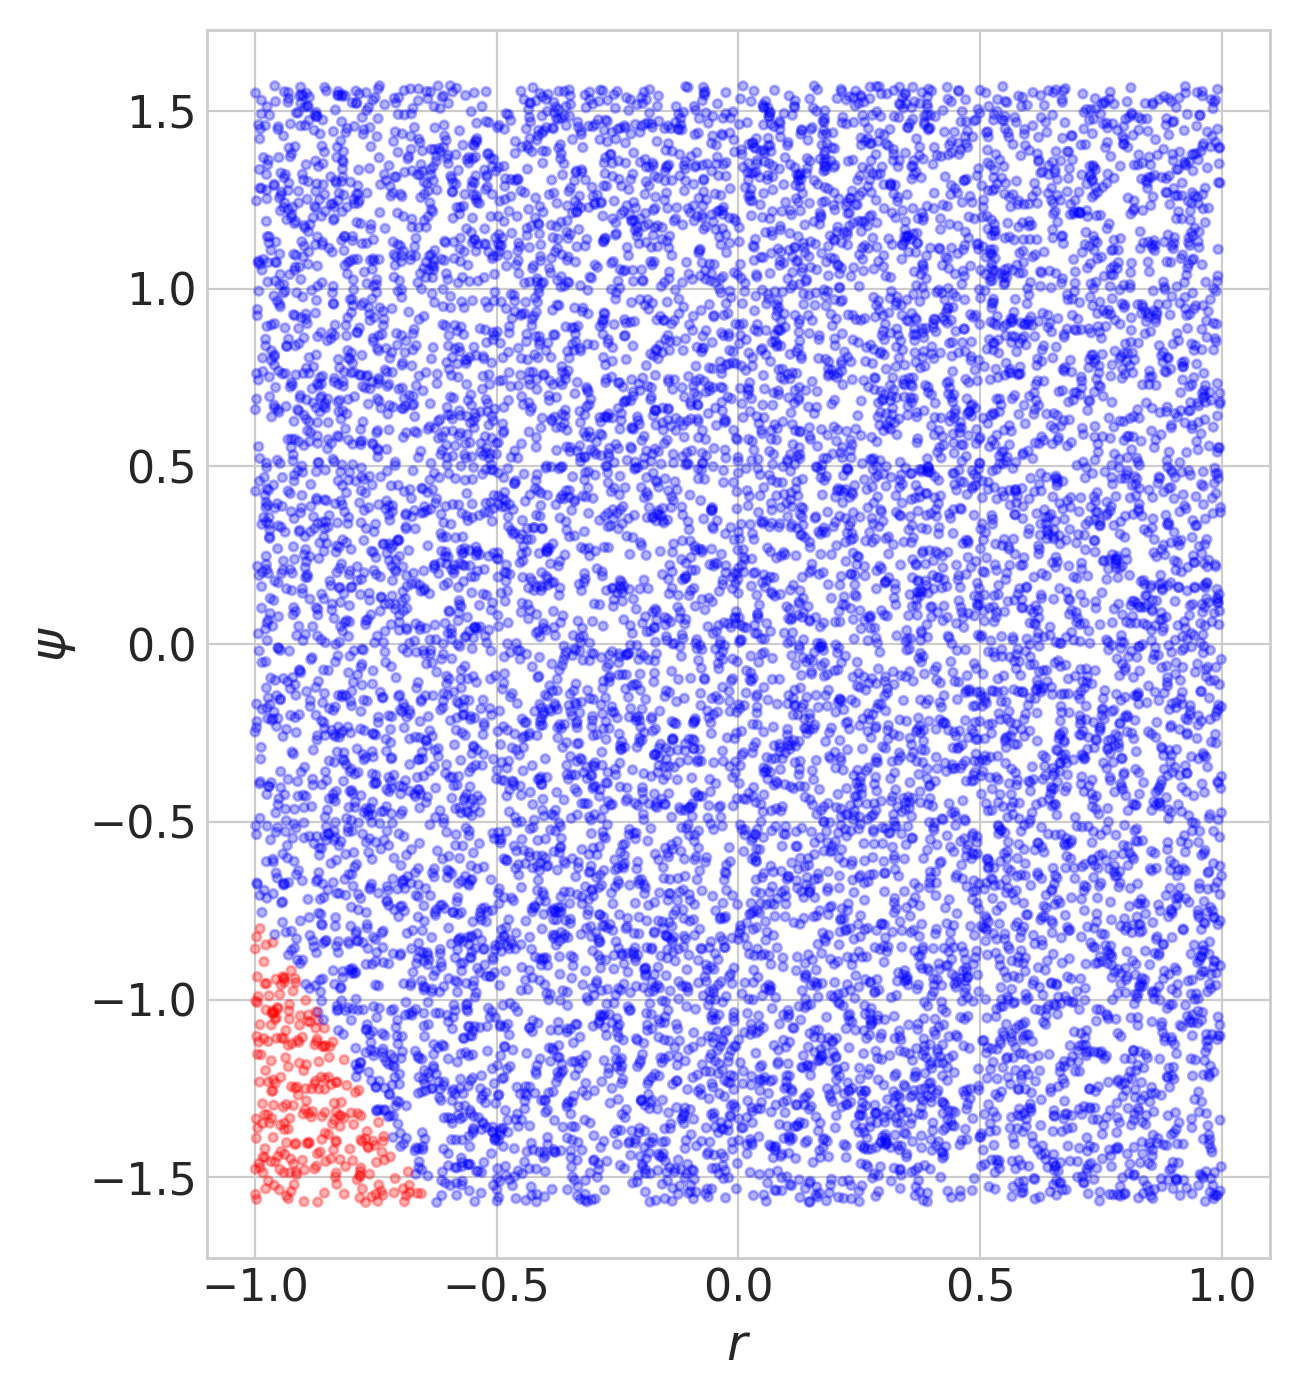
\includegraphics[width=.42\linewidth]{06_aplicacion_y_evaluacion_de_metodos_rl/stability_r-psi_th-0_5_t--1_ord-inf_ex-uvxy.png}%
            \label{subfig:psi}%
        }
        \caption{Cada gráfica de las \crefrange{subfig:z}{subfig:psi} representan las regiones de estabilidad encontradas a partir de $10,000$ simulaciones usando el controlador por retroalimentación de estados descrito en el algoritmo \ref{alg:Control_retro} en cada uno de los conjuntos mencionados. Cada coordenada marcada en azul representa una condición inicial a partir de las cuál su correspondiente trayectoria al tiempo $t=30$ cumplió el criterio de estabilidad \ref{eq:lin_creteria} con $\epsilon=0.5$. Las coordenadas rojas corresponden a trayectorias inestables.} 
        \label{fig:stability_region_linear}
\end{figure*}
    
\subsubsection{Regiones de estabilidad para \acrshort{ilqr}}
Este método tiene una capacidad de control sobre todas la coordenadas \ref{eq:quad_position} asociadas al sistema dinámico completo. Por lo que el criterio se aplicará sobre el estado completo del cuadricoptero, eso es equivalente a la siguiente expresión,
    \begin{align}
    \label{eq:ilqr_criteria}
        \|\mathbf{x}\|_{\infty} < \epsilon \qquad \epsilon > 0.
    \end{align}
En este caso se aplico el criterio sobre todos los conjuntos de condiciones iniciales. Los resultados se exhiben en el cuadro \ref{tab:stability_region_ilqr} 

\begin{table}[H]
\centering
\begin{tabular}{|c|c|c|c|c|}
\hline
\multirow{2}{*}{Conjunto} & \multirow{2}{*}{Rango} & \% trayectorias estables \\ 
                          &                          & $t=30$                        \\ \hline
$\chi_{ux}$ & $\pm\text{10.0},\quad\pm\text{20.0}$ & 52.0       \\
$\chi_{vy}$ & $\pm\text{10.0},\quad\pm\text{20.0}$ & 40.0       \\
$\chi_{wz}$ & $\pm\text{10.0},\quad\pm\text{20.0}$ & 95.0       \\
$\chi_{p\phi}$ & $\pm\text{1.0},\quad\pm\pi/2$ & 14.0 \\
$\chi_{q\theta}$ & $\pm\text{1.0},\quad\pm\pi/2$ & 22.0 \\
$\chi_{r\psi}$ & $\pm\text{1.0},\quad\pm\pi/2$ & 93.0 \\
total         & --            & 53.0 \\
\hline
\end{tabular}
\caption{Tasas de trayectorias estables generadas por el controlador ajustado por \acrshort{ilqr} hasta el segundo $30$ cuya región de estabilidad es mostrada en la figura \ref{fig:stability_region_ilqr}}
\label{tab:stability_region_ilqr}
\end{table}

\begin{figure}[h!]
\centering
\includegraphics[width=1.0\linewidth]{06_aplicacion_y_evaluacion_de_metodos_rl/stability_th-0_5_t--1_ord-inf.png}
\caption{Regiones de estabilidad sobre los conjuntos $\chi_{vy}$, $\chi_{wz}$, $\chi_{p\varphi}$, $\chi_{q\theta}$ y $\chi_{r\psi}$ del controlador \acrshort{ilqr} determinadas por el criterio \ref{eq:ilqr_criteria} en el tiempo $t=30$ con $\epsilon = 0.5$.}
\label{fig:stability_region_ilqr}
\end{figure}


\subsubsection{Regiones de estabilidad para \acrshort{gps}}
A pesar de que la estrategia de control de este método fue entrenada a partir de controladores \acrshort{ilqr}, como se mostró en el cuadro \ref{tab:percentiles_state_gps}, la política no parece tener un control efectivo sobre la coordenada $\psi$ a diferencia del resto de posiciones angulares. En consecuencia, el criterio que se usará excluye a las variables $\psi$ y $r$,
    \begin{align}
    \label{eq:gps_criteria}
        \|[u, v, w, x, y, z, p, q, \varphi, \theta]^{\top}\|_{\infty} < \epsilon \qquad \epsilon > 0.
    \end{align}
En este caso sí se tomaron en cuenta todos los conjuntos de prueba. Para validar la independencia con respecto al tiempo de la política \acrshort{gps} se consideraron distintos tiempos de corte para analizar, se usaron $15, 30$ y $60$ segundos. Los resultados se muestran en el cuadro \ref{tab:stability_region_gps}.

\begin{table}[H]
\centering
\begin{tabular}{|c|c|c|c|c|}
\hline
\multirow{2}{*}{Conjunto} & \multirow{2}{*}{Rango} & \multicolumn{3}{c|}{\% de trayectorias estables} \\ \cline{3-5}
                          &                          & $t=15$ & $t=30$ & $t=60$                       \\ \hline
$\chi_{ux}$ & $\pm\text{10.0},\quad\pm\text{20.0}$ & 20.0 & 24.0  & 25.0       \\
$\chi_{vy}$ & $\pm\text{10.0},\quad\pm\text{20.0}$ & 24.0 & 33.0  & 33.0       \\
$\chi_{wz}$ & $\pm\text{10.0},\quad\pm\text{20.0}$ & 42.0 & 43.0  & 43.0      \\
$\chi_{p\phi}$ & $\pm\text{1.0},\quad\pm\pi/2$ & 5.0 & 6.0  & 6.0\\
$\chi_{q\theta}$ & $\pm\text{1.0},\quad\pm\pi/2$ & 3.0 & 4.0  & 4.0\\
$\chi_{r\psi}$ & $\pm\text{1.0},\quad\pm\pi/2$ & 68.0 & 70.0  & 56.0\\
total         & --            & 27.0 & 30.0  & 28.0 \\
\hline
\end{tabular}
\caption{El porcentaje de trayectorias estables generadas por la política entrenada con el método \acrshort{gps} en los segundos $15$, $30$ y $60$ cuyas regiones son mostradas en las figuras \ref{fig:stability_region_15}, \ref{fig:stability_region_30} y \ref{fig:stability_region_60}, respectivamente.}
\label{tab:stability_region_gps}
\end{table}

\begin{figure}[h!]
\centering
\includegraphics[width=1.0\linewidth]{06_aplicacion_y_evaluacion_de_metodos_rl/stability_th-0_5_t-15_ord-inf_ex-rpsi.png}
\caption{Regiones de estabilidad sobre los conjuntos $\chi_{vy}$, $\chi_{wz}$, $\chi_{p\varphi}$, $\chi_{q\theta}$ y $\chi_{r\psi}$ del controlador \acrshort{gps} determinadas por el criterio \ref{eq:gps_criteria} en el tiempo $t=15$ con $\epsilon = 0.5$.}
\label{fig:stability_region_15}
\end{figure}

\newpage
\begin{figure}[h!]
\centering
\includegraphics[width=1.0\linewidth]{06_aplicacion_y_evaluacion_de_metodos_rl/stability_th-0_5_t-30_ord-inf_ex-rpsi.png}
\caption{Regiones de estabilidad sobre los conjuntos $\chi_{vy}$, $\chi_{wz}$, $\chi_{p\varphi}$, $\chi_{q\theta}$ y $\chi_{r\psi}$ del controlador \acrshort{gps} determinadas por el criterio \ref{eq:gps_criteria} en el tiempo $t=30$ con $\epsilon = 0.5$.}
\label{fig:stability_region_30}
\end{figure}
 
\begin{figure}[h!]
\centering
\includegraphics[width=1.0\linewidth]{06_aplicacion_y_evaluacion_de_metodos_rl/stability_th-0_5_t-60_ord-inf_ex-rpsi.png}
\caption{Regiones de estabilidad sobre los conjuntos $\chi_{vy}$, $\chi_{wz}$, $\chi_{p\varphi}$, $\chi_{q\theta}$ y $\chi_{r\psi}$ del controlador \acrshort{gps} determinadas por el criterio \ref{eq:gps_criteria} en el tiempo $t=60$ con $\epsilon = 0.5$.}
\label{fig:stability_region_60}
\end{figure}

\newpage
\subsubsection{Regiones de estabilidad para \acrshort{ddpg}}
Como se mostró en el cuadro \ref{tab:ddpg_coordinates_dispersion} la política entrenada \acrshort{ddpg} no mostró un control efectivo sobre las variables $w, x, y, z, r$ y $\psi$. Por lo que el criterio que se usó excluye estas variables, 
\begin{align}
    \|[u, v, p,q,\phi,\theta]^{\top}\|_{\infty} < 0.5. 
\end{align}
Al igual que para el criterio \acrshort{gps} se consideraron los conjuntos de condiciones iniciales $\mathcal{X}_{ux}, \mathcal{X}_{vy}, \mathcal{X}_{wz}, \mathcal{X}_{p\varphi}, \mathcal{X}_{q\theta}$ y $\mathcal{X}_{r\psi}$. También se validó la independencia de la política con respecto al tiempo al aplicar el criterio sobre los cortes de 15, 30 y 60 segundos. Los resultados se muestran en el cuadro \ref{tab:stability_region_ddpg}. 

\begin{table}[H]
\centering
\begin{tabular}{|c|c|c|c|c|}
\hline
\multirow{2}{*}{Conjunto} & \multirow{2}{*}{Rango} & \multicolumn{3}{c|}{\% de trayectorias estables} \\ \cline{3-5}
                          &                          & $t=15$ & $t=30$ & $t=60$                       \\ \hline
$\chi_{ux}$ & $\pm\text{10.0},\quad\pm\text{20.0}$ & 0.0 & 0.0015  & 0.0       \\
$\chi_{vy}$ & $\pm\text{10.0},\quad\pm\text{20.0}$ & 0.0008 & 0.0006  & 0.0004       \\
$\chi_{wz}$ & $\pm\text{10.0},\quad\pm\text{20.0}$ & 0.0 & 0.0  & 0.0      \\
$\chi_{p\phi}$ & $\pm\text{1.0},\quad\pm\pi/2$ & 0.0 & 0.0  & 0.0\\
$\chi_{q\theta}$ & $\pm\text{1.0},\quad\pm\pi/2$ & 0.0 & 0.0  & 0.0\\
$\chi_{r\psi}$ & $\pm\text{1.0},\quad\pm\pi/2$ & 0.0 & 0.0  & 0.0\\
total         & --            & 0.0 & 0.0  & 0.0 \\
\hline
\end{tabular}
\caption{El porcentaje de trayectorias estables generadas por la política entrenada con el método \acrshort{ddpg} en los segundos $15$, $30$ y $60$.}
\label{tab:stability_region_ddpg}
\end{table}



\chapter{Conclusión}

En este trabajo se utilizaron los métodos de \acrshort{rl}: \acrshort{gps} (\textit{model-based}) y \acrshort{ddpg} (\textit{model-free}) para optimizar diferentes \acrshort{ann} con el propósito de controlar un cuadricoptero, llevarlo al origen alineado con los ejes, con velocidades angulares y lineales iguales a cero, tal como lo hace un controlador \acrshort{ilqr}. De hecho, se uso el método \acrshort{ilqr} para conseguir una configuración subóptima del costo, que fue fundamental para los métodos de \acrshort{rl}. El primer entrenamiento se realizó con el método \acrshort{gps}, debido a que el uso de controladores locales \acrshort{ilqr} generaba mayor certeza en los resultados. Esto a su vez permitió definir una arquitectura de la \acrshort{ann} asociada a la política e hiperparametros que después serian retomados en el método \acrshort{ddpg}. 

Para el método \acrshort{ddpg} se utilizó una configuración mucho más flexible que el costo de \acrshort{gps} con la finalidad de recompensar un comportamiento deseado y penalizar uno no deseado. 

Una vez entrenadas las diferentes políticas con los métodos \acrshort{gps} y \acrshort{ddpg} se definieron conjuntos para probar la estabilidad y distintos al usado en el entrenamiento para determinar la confiabilidad de estos métodos. Esto dio lugar a una comparación no estricta de los métodos basados en redes neuronales con los métodos de control más convencionales: \acrshort{ilqr} y control linealizado por retroalimentación. Se observa en las figuras \ref{fig:stability_region_ilqr} y \ref{fig:stability_region_linear} que bajo sus respectivos criterios ambos controladores convencionales generan regiones conexas de posiciones iniciales cuyas trayectorias correspondientes terminaron cerca del objetivo. 

La política resultante de \acrshort{gps} imitó el comportamiento del controlador \acrshort{ilqr} todas las variables salvo en el ángulo $\psi$ y velocidad $r$ en muestras de la distribución $\mathcal{X}$, como se observa en \ref{fig:state_traj_gps}. Al excluir esas variables, la política genera una cantidad de trayectorias estables, incluso varias fuera de las regiones conexas de los métodos convencionales. Se destaca que en el eje $(r-\psi)$ se observa un alto porcentaje de estabilidad en los rangos de perturbación definidos, mientras que en los ejes angulares $(p-\varphi)$ y $(q-\theta)$ son mínimas las trayectorias estables. Sin embargo, en general no se encontraron regiones conexas que permitan determinar la confiabilidad de la política. 

El método \acrshort{ddpg} falla en la tarea fijada en este trabajo, esto puede deberse al mecanismo descrito en \textit{The problem with DDPG: understanding failures in deterministic environments with sparse rewards} \cite{Matheron2020}. El algoritmo parece entrar en punto fijo subóptimo. La región de acciones que estabilizan el cuadricoptero es muy estrecha y la recompensa, aunque formalmente es densa, es efectivamente escasa (debido a $\tanh^2$). Esto fomenta que el actor converja rápidamente a una política de acciones constantes antes de haber observado transiciones relevantes. Entonces el crítico converge a una función de valor plana. El sistema entra así en un \textit{deadlock} actor-crítico descrito en \cite{Matheron2020}. El actor no puede cambiar porque el gradiente es nulo, y el crítico no generaliza a mejores acciones, esto hace que \acrshort{ddpg} quede atrapado en un política incapaz de estabilizar el cuadricoptero. Esta caracterización se hace patente en las acciones mostradas en la figura \ref{fig:ddpg_actions}. Se observa que con $10$ \textit{epochs} el entrenamiento no es suficiente para obtener una política efectiva; sin embargo, con una mayor cantidad de epochs–como 200– la política sigue siendo inefectiva y es prácticamente constante. 

Este trabajo echibe que los métodos \acrshort{ddpg} y \acrshort{gps} son flexibles, fuertemente adaptativos a las nuevas experiencias, potencialmente útiles para aprender tareas complejas como se demuestra \cite{hwangbo2017control}, \cite{zhang2016}. Precisamente estos dos trabajos persiguen un enfoque híbrido entre \acrshort{rl}, el uso de redes neuronales y métodos más convencionales de control. Por si sólo \acrshort{gps} ya es un enfoque híbrido. Sin embargo, en el caso del control de un cuadricoptero, las políticas entrenadas no es suficiente para generar trayectorias estables en diferentes perturbaciones, esto puede deberse a la la complejidad de la dinámica. A pesar de ello este trabajo sirve preámbulo para adentrarse comprender el método \acrshort{mpc}-\acrshort{gps} \cite{zhang2016}, que resuelve el problema de generar trayectorias y evitar objetos por parte de un cuadricoptero. Esto sugiere que este método podría llevar acabo con mejor efectividad las pruebas de estabilidad presentadas aquí. También este trabajo muestra las limitaciones del método \acrshort{ddpg} para entrenar por si sólo una política que cumpla el objetivo planteado. Sin embargo, esto puede dar lugar a usar métodos más robustos y estables como \acrshort{td3} \cite{fujimoto2018} o \acrshort{sac} \cite{haarnoja2018}, así como explorar estrategias híbridas preservando el enfoque \textit{model-free}. 

\appendix



% -----------------------------------------------------------------------
% Appendices
% -----------------------------------------------------------------------
\appendix

\chapter{Hiperparámetros}
\section{Configuración de entorno}
\begin{table}[h]
\centering
\begin{tabular}{|l|l|l|}
\hline
\textbf{Símbolo} & \textbf{Significado} & \textbf{Valor} \\ \hline
$T$ & Número de pasos de tiempo de simulación & 750  \\ \hline
$\Delta t$ & Tamaño de paso de simulación & 0.04 \\ \hline
– & Tiempo de simulación en segundos & 30  \\ \hline
\end{tabular}
\end{table}

\section{Búsqueda de línea \& regularización (\acrshort{ilqr})}
\begin{table}[H]
\centering
\begin{tabular}{|l|l|l|}
\hline
\textbf{Símbolo} & \textbf{Significado} & \textbf{Valor} \\ \hline
– & Número de actualizaciones máximas & 100 \\ \hline
$\bm{\alpha}$ & Factores de búsqueda de línea & $\left\{\frac{1}{2}^{i}\right\}_{i=0}^{7}$ \\ \hline
$\lambda_0$ & Regularización inicial (Levenberg–Marquardt) & 20 \\ \hline
$\lambda_{\min}$ & Regularización mínima permitida & $10^{-3}$ \\ \hline
$\lambda_{\max}$ & Regularización máxima permitida & $10^{4}$ \\ \hline
$\Delta_{0}$ & Factor inicial de ajuste de regularización & 2 \\ \hline
$\epsilon_{tol}$ & Tolerancia de convergencia & 0.1 \\ \hline
\end{tabular}
\end{table}

\section{\acrshort{ddpg}}
\begin{table}[H]
\centering
\begin{tabular}{|l|l|l|}
\hline
\textbf{Símbolo} & \textbf{Significado} & \textbf{Valor} \\ \hline
– & Optimizador & \acrshort{adam}  \\ \hline
$K$ & Episodios & 10  \\ \hline
– & Pasos por episodio & 80  \\ \hline
– & Prueba por episodio & 1 \\ \hline
$\alpha_{\mu}$ & Tasa de aprendizaje de \textit{actor} & $10^{-4}$ \\ \hline
$\alpha_{Q}$ & Tasa de aprendizaje de \textit{critic} & $10^{-3}$ \\ \hline
$L$ & Número de capas ocultas & 2 \\ \hline
$n_{\ell}$ & Neuronas por capa oculta & 128 \\ \hline 
– & Función de activación ($\bm\theta_{\mu}$)& \acrshort{relu} \\ \hline
– & Función de salida ($\bm\theta_{\mu}$) & $\tanh$ \\ \hline 
– & Función de activación ($\bm\theta_{Q}$)& \acrshort{relu} \\ \hline
– & Función de salida ($\bm\theta_{Q}$) & lineal \\ \hline
$\gamma$ & Tasa de descuento & 0.99 \\ \hline
$N$ & Tamaño \textit{mini-batch} & 128 \\ \hline
$|\mathcal{D}|$ & Tamaño de \textit{buffer} & $10^{4}$ \\ \hline
$\tau$ & Coeficiente de actualización suave & $10^{-3}$ \\ \hline
\end{tabular}
\end{table}

\subsection{\acrshort{ou}}
\label{tab:ou_noise}
\begin{table}[H]
\centering
\begin{tabular}{|l|l|l|}
\hline
\textbf{Símbolo} & \textbf{Significado} & \textbf{Valor} \\\hline
$\mu$ & Media a largo plazo & 0.0 \\ \hline
$\theta$ & Tasa de reversión a la media & 0.15 \\ \hline
$\sigma_{\text{max}}$ & Volatilidad inicial (máxima) & 0.3 \\ \hline
$\sigma_{\text{min}}$ & Volatilidad final (mínima) & 0.01 \\ \hline
\end{tabular}
\end{table}

\section{\acrshort{gps}}
\begin{table}[h]
\centering
\begin{tabular}{|l|l|l|}
\hline
\textbf{Símbolo} & \textbf{Significado} & \textbf{Valor} \\ \hline
$K$ & Número de pasos de entrenamiento & 5 \\ \hline
$N$ & Número de controladores locales & 7 \\ \hline
$M$ & Número de trayectorias simuladas por controlador & 800 \\ \hline
$\epsilon$ & Cota de divergencia \acrshort{kl} entre política y controladores & 3000 \\ \hline
$\eta_{\min}$ & Valor mínimo de penalización de \acrshort{kl} & 1 \\ \hline
$\eta_{\max}$ & Valor máximo de penalización de \acrshort{kl} & $10^{4}$ \\ \hline
$\nu_t^{(\text{init})}$ & Factor de regularización inicial para la dinámica local & $10^{-3}$ \\ \hline
$\alpha_{\bm\lambda}$ & Tasa de aprendizaje del multiplicador de Lagrange & $10^{-2}$ \\ \hline
– & Optimizador& \acrshort{adam} \\ \hline
$\alpha$ & Tasa de aprendizaje de política& 0.001 \\ \hline
$L$ & Número de capas ocultas & 2 \\ \hline
$n_{\ell}$ & Neuronas por capa oculta & 128 \\ \hline 
– & Función de activación de política & \acrshort{relu} \\ \hline
– & Función de salida de política & $\tanh$ \\ \hline
\end{tabular}
\end{table}



\chapter{Redes neuronales artificiales}
\label{appendix:DL}

En gran medida el éxito de la inteligencia artificial se debe al desarrollo del \textbf{aprendizaje profundo}, mejor conocido como \textbf{\acrfull{dl}}. El aprendizaje profundo utiliza \textbf{redes neuronales artificiales} como modelo subyacente para la inteligencia artificial \cite{Roberts_2022}. Las redes neuronales artificiales son estructuras paramétricas adaptativas que procesan información. Se les denomina redes porque están compuestas por múltiples funciones y se les suele asociar con gráficas acíclicas \cite{Goodfellow-et-al-2016}. Aunque este modelo tuvo su inspiración en la neurociencia, hoy en día guarda poca relación con ese campo de estudio \footnote{El concepto de neurona artificial fue concebido por McCulloch y Pitts en 1943 como un modelo de una neurona biológica \cite{Roberts_2022}. Posteriormente, en 1958 Rosenblatt introdujo el modelo perceptrón, que incorpora el uso de parámetros ajustables \cite{Roberts_2022}. El modelo de perceptrón fue el primer cimiento del aprendizaje profundo.}. En la actualidad, las redes neuronales artificiales son máquinas de aproximación de funciones que están diseñadas para lograr generalización estadística \cite{Goodfellow-et-al-2016}. 

\section{Redes unidireccionales}
Para este trabajo sólo será necesario introducir una clase de red neuronal artificial, conocida como \textbf{perceptrón multicapa}, también denominado \acrfull{mlp}. Un \acrshort{mlp} es una función paramétrica adaptativa que tiene el fin de aproximar otra función. Este tipo de redes neuronales tiene la cualidad de que los valores de entrada sólo se propagan en una dirección y no generan ciclos internamente \cite{Roberts_2022}. Por esta razón también se les conoce como \textbf{redes unidireccionales} (\textit{feedforward}). En este trabajo se usa el término \acrfull{ann} para referirse a un \acrshort{mlp}.

En esta sección se definen los principales elementos de una \acrshort{ann} unidireccional, como  neuronas, funciones de activación, parámetros y capas (\textit{layers}). Todos estos elementos se agrupan en una estructura llamada arquitectura.


\subsection{Arquitectura}
\label{sec:ann_architecture}
La arquitectura se define como la topología, estructura u organización de la \acrshort{ann}. Dicha arquitectura se compone de neuronas o nodos, que son conectados por medio de un enlace. Este enlace es direccional y representa la trayectoria que debe seguir la información. Las neuronas se agrupan en unidades estructurales llamadas capas. \cite{Goodfellow-et-al-2016}

La siguiente definición está basada en lo mostrado en \cite{Roberts2022}.

\begin{definition}
\label{def:ANN}
Una \textbf{red neuronal unidireccional completamente conectada} está descrita por su arquitectura $a = \langle N, \phi \rangle$, donde $N \in \mathbb{N}^{L+1}$ es un arreglo que representa a la cantidad de nodos en cada capa, $L \in \mathbb{N}$ representa al número de capas y $\phi : \mathbb{R} \rightarrow \mathbb{R}$ se refiere a la función de activación. Sean $n_0$, $n_L$ y $n_{\ell} \in \mathbb{N}$ el número de neuronas en la capa de entrada, salida y $\ell$-ésima, respectivamente. Sea $f_a(\cdot ;\bm{\theta}): \mathbb{R}^{n_0} \rightarrow \mathbb{R}^{n_L}$ la función correspondiente a la \acrshort{ann}, que para todo valor $\mathbf{x} \in \mathbb{R}^{n_0}$ y parámetros
$$
\bm{\theta} = \left(\mathbf{W}^{[\ell]}, \mathbf{b}^{[\ell]}\right)_{\ell =1}^{L} \in \Theta,
$$
se expresa de la siguiente forma,
%Sea $L\in \mathbb{N}$ con $L \geq 2$ y sean $n_0$ y $n_L \in \mathbb{N}$. Sea $\mathcal{N}(\cdot | \theta):\mathbb{R}^{n_0} \rightarrow \mathbb{R}^{n_L}$ un \textbf{perceptrón multicapa unidireccional} con $L$ capas, parámetros $\theta$ y función de activación $\phi$, que se define de la siguiente manera: 
\begin{align}
f_a(\textbf{x}; \bm{\theta}) := \phi\circ(T_{L}(\phi\circ(T_{L-1}(\cdots \phi\circ(T_1(\mathbf{x})) \cdots)))).
\label{eq:ANN}
\end{align}
donde,
$$
\Theta := \prod_{\ell=1}^{L}
\left(
\mathbb{R}^{n_{\ell}\times n_{\ell-1}} \times \mathbb{R}^{n_{\ell}}
\right).
$$
 La expresión $T_{\ell}$ representa la transformación aplicada al valor de salida $\mathbf{z} \in \mathbb{R}^{n_{
 \ell -1}}$ de la capa anterior.
 Esta transformación está dada por la siguiente expresión,
$$T_{\ell}(\mathbf{z}) = \mathbf{W}^{[\ell]}\mathbf{z} + \mathbf{b}^{[\ell]} \qquad \mathbf{W}^{[\ell]} \in \mathbb{R}^{n_{\ell} \times n_{\ell -1}}, \mathbf{b}^{[\ell]} \in \mathbb{R}^{n_{\ell}} \qquad \forall \ell \in \{1, 2, \cdots, L\}.$$
La función de escalar $\phi: \mathbb{R} \rightarrow \mathbb{R}$ se denomina función de activación y el operador $\circ$ representa que la operación se realiza elemento por elemento.
%Sean $\textbf{x}\in \mathbb{R}^{1 \times n_x}$, $\textbf{y} \in \mathbb{R}^{1 \times n_y}$ y $W^{[\ell]} \in \mathbb{R}^{n_{\ell} \times n_{\ell - 1}}$ donde $\ell$ representa el índice de capa, $n_{\ell-1}$ y $n_{\ell}$ son las dimensiones de entrada y salida de la capa $\ell$, respectivamente.
\end{definition}
Una \acrshort{ann} está completamente caracterizada por su arquitectura $a = \langle N, \phi \rangle$ y sus parámetros $\bm\theta$, es decir, que basta con conocer la cantidad de capas, su dimensión y la función de activación que se aplica a cada neurona para saber la forma de la \acrshort{ann}. Cuando no sea necesario hacer énfasis sobre la arquitectura de la \acrshort{ann}, se omite en la notación de tal forma que $f_a(\mathbf{x}; \bm{\theta})=f(\mathbf{x}; \bm{\theta})$.

En este caso una neurona se refiere a la aplicación de la transformación $T_{\ell}$ y la subsecuente aplicación de su correspondiente función de activación $\phi$ sobre uno de los valores de salida $\mathbf{z}_j$ de la capa anterior. Esta interpretación de las neuronas como módulos unitarios se hace patente en la representación gráfica de una \acrshort{ann} como se muestra en la figura \ref{fig:multilayer-perceptron}.

\subsubsection{Función de activación}
Usualmente la función de activación se escoge como una función no lineal con el fin de incrementar la expresividad de una \acrshort{ann} \cite{Roberts_2022}. Sin una función de activación o con una función de activación lineal, el mapeo definido por una \acrshort{ann} de la forma en la \eqreftext{eq:ANN} se restringiría a ser lineal \cite{prince2023understanding}. A continuación se muestran las funciones de activación comúnmente empleadas. 

\begin{example}
Sea $\phi: \mathbb{R} \rightarrow [-1, 1]$ la función de activación dada por la siguiente expresión,
$$\phi(x) = \left(\frac{e^{x} -e^{-x}}{e^{x} + e^{-x}}\right).$$
Esta función es denominada como \textbf{tangente hiperbólica}.
\end{example}

\begin{example}
Sea $\phi: \mathbb{R} \rightarrow \mathbb{R}$ la función de activación llamada \textbf{\acrfull{relu}}. Está dada por la siguiente expresión,
$$\phi(x) = 
\begin{cases}
0 & \text{ si } x<0, \\
x & \text{e.o.c.}
\end{cases}
.
$$
\end{example}

%La concatenación de capas de $\mathcal{N}$ se puede desglosar de la siguiente manera:

\begin{figure}[t]
	\centering
	\begin{tikzpicture}[shorten >=1pt]
	    \tikzstyle{unit}=[draw,shape=circle,minimum size=1.15cm]
	    %\tikzstyle{hidden}=[draw,shape=circle,fill=black!25,minimum size=1.15cm]
	    \tikzstyle{hidden}=[draw,shape=circle,minimum size=1.15cm]
 
	    \node[unit](x0) at (0,3.5){$x_1$};
	    \node[unit](x1) at (0,2){$x_2$};
	    \node at (0,1){\vdots};
	    \node[unit](xd) at (0,0){$x_{n_0}$};
 
	    \node[hidden](h10) at (3,4){$h_1^{[1]}$};
	    \node[hidden](h11) at (3,2.5){$h_2^{[1]}$};
	    \node at (3,1.5){\vdots};
	    \node[hidden](h1m) at (3,-0.5){$h_{n_1}^{[1]}$};
 
	    \node(h22) at (5,0){};
	    \node(h21) at (5,2){};
	    \node(h20) at (5,4){};
	    
	    \node(d3) at (6,0){$\ldots$};
	    \node(d2) at (6,2){$\ldots$};
	    \node(d1) at (6,4){$\ldots$};
 
	    \node(hL12) at (7,0){};
	    \node(hL11) at (7,2){};
	    \node(hL10) at (7,4){};
	    
	    \node[hidden](hL0) at (9,4){$h_1^{[L]}$};
	    \node[hidden](hL1) at (9,2.5){$h_2^{[L]}$};
	    \node at (9,1.5){\vdots};
	    \node[hidden](hLm) at (9,-0.5){$h_{n_{L}}^{[L]}$};
 
	    \node[unit](y1) at (12,3.5){$y_1$};
	    \node[unit](y2) at (12,2){$y_2$};
	    \node at (12,1){\vdots};	
	    \node[unit](yc) at (12,0){$y_{n_{L+1}}$};
	    
        \draw[-] (x0) -- (h10);
	    \draw[-] (x0) -- (h11);
	    \draw[-] (x0) -- (h1m);
 
        \draw[-] (x1) -- (h10);
	    \draw[-] (x1) -- (h11);
	    \draw[-] (x1) -- (h1m);
        
        \draw[-] (xd) -- (h10);
	    \draw[-] (xd) -- (h11);
	    \draw[-] (xd) -- (h1m);
 
	    \draw[-] (hL0) -- (y1);
	    \draw[-] (hL0) -- (yc);
	    \draw[-] (hL0) -- (y2);
 
	    \draw[-] (hL1) -- (y1);
	    \draw[-] (hL1) -- (yc);
	    \draw[-] (hL1) -- (y2);
 
	    \draw[-] (hLm) -- (y1);
	    \draw[-] (hLm) -- (y2);
	    \draw[-] (hLm) -- (yc);
 
	    \draw[-,path fading=east] (h10) -- (h21);
	    \draw[-,path fading=east] (h10) -- (h22);
	    \draw[-,path fading=east] (h10) -- (h20);
	    
	    \draw[-,path fading=east] (h11) -- (h21);
	    \draw[-,path fading=east] (h11) -- (h22);
	    \draw[-,path fading=east] (h11) -- (h20);
	    
	    \draw[-,path fading=east] (h1m) -- (h21);
	    \draw[-,path fading=east] (h1m) -- (h22);
	    \draw[-,path fading=east] (h1m) -- (h20);
	    
	    \draw[-,path fading=west] (hL10) -- (hL1);
	    \draw[-,path fading=west] (hL11) -- (hL1);
	    \draw[-,path fading=west] (hL12) -- (hL1);
	    
	    \draw[-,path fading=west] (hL10) -- (hLm);
	    \draw[-,path fading=west] (hL11) -- (hLm);
	    \draw[-,path fading=west] (hL12) -- (hLm);
	    
	    \draw [decorate,decoration={brace,amplitude=10pt},xshift=-4pt,yshift=0pt] (-0.5,4) -- (0.75,4) node [black,midway,yshift=+0.6cm]{valores de entrada};
	    \draw [decorate,decoration={brace,amplitude=10pt},xshift=-4pt,yshift=0pt] (2.5,4.5) -- (3.75,4.5) node [black,midway,yshift=+0.6cm]{primera capa oculta};
	    \draw [decorate,decoration={brace,amplitude=10pt},xshift=-4pt,yshift=0pt] (8.5,4.5) -- (9.75,4.5) node [black,midway,yshift=+0.6cm]{$L$-esima capa oculta};
	    \draw [decorate,decoration={brace,amplitude=10pt},xshift=-4pt,yshift=0pt] (11.5,4) -- (12.75,4) node [black,midway,yshift=+0.6cm]{capa de salida};
	\end{tikzpicture}
	\caption{Red que representa un perceptrón multicapa de $L$ capas ocultas con $n_0$ valores de entrada y $n_{L+1}$ valores de salida. La $L$-esima capa oculta recibe $n_{L}$ valores de la capa anterior. En este caso $h_{n}^{[\ell]} = \phi\left(\mathbf{W}^{[\ell]}\mathbf{h}_{m}^{[\ell -1]} + \mathbf{b}^{[\ell]}\right) $ representa la $n$-ésima salida de la $\ell$-ésima capa de la \acrshort{ann}, donde $1 \leq \ell \leq L$.}	
 \label{fig:multilayer-perceptron}
\end{figure}

\section{Entrenamiento}
El entrenamiento de una \acrshort{ann} se refiere al proceso de encontrar los parámetros óptimos para la tarea que realiza. Este proceso también se suele denominar aprendizaje. Para encontrar estos valores, existen múltiples técnicas, la más común ha sido hacer uso de la optimización basada en gradientes. \cite{Goodfellow-et-al-2016}

Los algoritmos de aprendizaje basados en gradientes tienen la capacidad de eficientemente procesar datos de entrenamiento al optimizar una función objetivo o pérdida que directamente mide el desempeño de la \acrshort{ann} para una tarea específica. En particular, una función de pérdida puede comparar la salida del mapeo de la \acrshort{ann} con el valor deseado o etiqueta \cite{Roberts_2022}, este enfoque se denomina aprendizaje supervisado.

\subsection{Aprendizaje supervisado}
\label{sec:supervised_learning}
En términos generales los algoritmos que conforman el paradigma de aprendizaje supervisado tiene el objetivo de encontrar una relación verosímil entre los valores de una imagen y un dominio \cite{prince2023understanding}. Concretamente, dada una distribución de datos $(\textbf{x}, \textbf{y})$, el objetivo es enseñar a un modelo a asociar algún valor $\textbf{x}$ con una \textbf{etiqueta} $\textbf{y}$ \cite{Goodfellow-et-al-2016}. Al proceso de usar valores de la imagen para encontrar su correspondiente elemento en el dominio por medio de la ecuación se le conoce como \textbf{inferencia} \cite{prince2023understanding}. 

Antes de describir el proceso de entrenamiento, es necesario entender que significa que el modelo tiene un comportamiento adecuado. Esto quiere decir que dada una pareja $(\mathbf{x}, \mathbf{y})$ de la distribución de datos, la predicción del modelo $f(\mathbf{x}; \bm{\theta})$ se acerque lo más posible a la etiqueta $\mathbf{y}$ en promedio. Con el fin de medir esta cercanía se define la \textbf{función objetivo},
\begin{align}
\mathcal{L}\Big(f(\mathbf{x};\bm\theta), \mathbf{y}\Big),
\label{eq:loss_super}
\end{align}
tal que entre más cercano sea $f(\mathbf{x};\bm\theta)$ a $\mathbf{y}$, menor será el valor de la función objetivo. \cite{Roberts_2022}

La meta del entrenamiento es ajustar los parámetros del modelo de tal forma que permita reducir el valor en la \eqreftext{eq:loss_super} de tantas muestras como sea posible \cite{Roberts_2022}. Idealmente, se necesita reducir el valor esperado sobre toda la distribución de datos, 
\begin{align}
    \mathbb{E}[\mathcal{L}(\bm\theta)] = \int p(x, y)\mathcal{L}\Big(f(\mathbf{x};\bm\theta), \mathbf{y}\Big) dxdy .
    \label{eq:mean_loss}
\end{align}
Sin embargo, en la práctica no siempre se tiene acceso a una expresión analítica de la distribución de los datos \cite{Roberts_2022}. En lugar de ello, se usa una expresión \textbf{empírica} en la \eqreftext{eq:mean_loss}. Se muestrean un conjunto finito de datos $\mathcal{A}$ y se optimiza la siguiente función, 
\begin{align}
    \mathcal{L}_{\mathcal{A}}(\bm\theta) = \frac{1}{|\mathcal{A}|}\sum_{(\mathbf{x}, \mathbf{y}) \in \mathcal{A}} \mathcal{L}\Big(f(\mathbf{x};\bm\theta), \mathbf{y}\Big),
    \label{eq:train_loss}
\end{align}
el conjunto $\mathcal{A}$ se llama \textbf{conjunto de entrenamiento}.

Específicamente, entrenar una \acrshort{ann} consiste en encontrar una configuración de parámetros que minimice el valor de pérdida sobre todo el conjunto de entrenamiento, 
\begin{align}
    \bm\theta^{*} =\argmin_{\bm\theta}\mathcal{L}_{\mathcal{A}}(\bm\theta) = \argmin_{\bm\theta} 
    \left[
    \frac{1}{|\mathcal{A}|}
    \sum_{(\mathbf{x}, \mathbf{y}) \in \mathcal{A}} \mathcal{L}\Big(f(\mathbf{x};\bm\theta), \mathbf{y}\Big)
    \right].
    \label{eq:min_train_loss}
\end{align}
\subsection{Descenso por el gradiente}
\label{sec:gradient_decent}
Si la función objetivo en la \eqreftext{eq:train_loss} es diferenciable, revolver el problema de optimización planteado en la \eqreftext{eq:min_train_loss} es equivalente a encontrar el valor extremo $\bm\theta^{*}\in\Theta$ por medio de la siguiente ecuación,
$$\mathbf{0}=\nabla_{\bm\theta}\mathcal{L}_{\mathcal{A}}(\bm\theta).$$
Sin embargo, esta ecuación no puede resolverse directamente salvo en ciertos casos. En la práctica, en lugar de obtener una solución analítica se utilizan algoritmos iterativos que en cada paso reduzcan el error.

El método de \textbf{descenso por el gradiente} es un algoritmo de optimización de primer orden que comúnmente es utilizado para encontrar el mínimo de funciones utilizadas en aprendizaje automático como la \eqreftext{eq:train_loss} \cite{Roberts_2022}.
Para encontrar un mínimo de una función utilizando el descenso por el gradiente, se toman pasos actualización proporcionales al gradiente negativo de la misma función a partir del valor actual \cite{mml-book2020}.

En particular, en el aprendizaje profundo se utiliza una versión del método llamado \textbf{descenso por el gradiente estocástico}, cuya regla de actualización aplicado al problema en la \eqreftext{eq:min_train_loss} es,
\begin{align}
    \bm\theta^{(k+1)} = \bm\theta^{(k)} - \alpha \nabla_{\bm\theta}\mathcal{L}_{\mathcal{S}_{k}}(\bm\theta)\Big|_{\bm\theta = \bm\theta^{(k)}},
    \label{eq:SGD}
\end{align}
donde $k$ representa el número de actualizaciones anteriores. Cada $\mathcal{S}_{k}$ es llamado 
\textbf{\textit{batch}} o \textit{mini-batch} y representa una partición del conjunto de entrenamiento $\mathcal{A}$. En este caso el entrenamiento se divide en \textbf{épocas} (\textit{epochs}), una época consta de utilizar la regla en la \eqreftext{eq:SGD} sobre todos los \textit{mini-batches} que conforman el conjunto de entrenamiento. \cite{Roberts_2022} 






\chapter{Métodos Analíticos y Numéricos}
\label{appendix:metodos_numericos}

En este apéndice se presentan herramientas matemáticas complementarias utilizadas en el desarrollo de este trabajo. En particular, se incluye una introducción a la aproximación estocástica y un resultado sobre la divergencia de Kullback-Leibler para distribuciones normales multivariadas.

\section{Aproximación estocástica}
La aproximación estocástica se refiere a una amplia clase de métodos estocásticos iterativos que tienen el objetivo de encontrar raíces o resolver problemas de optimización. No obstante, la definición de estas tareas en muchas ocasiones implica estimar funciones desconocidas. \cite{Shiyu2022}

Para motivar el estudio de esta técnica y encontrar su relación con el aprendizaje por refuerzo, se retoma el ejemplo presentado en \cite{Shiyu2022}.

\subsection{Motivación}
Sea $Z$ una variable aleatoria. Se desea obtener una estimación del valor esperado $\mathbb{E}[Z]$. Con el fin de realizar la estimación, se considera un conjunto de muestras i.i.d $\{z_{i}\}$. Entonces, el valor esperado de $Z$ se aproxima por la siguiente expresión,
\begin{align}
    \mathbb{E}[Z] \approx \frac{1}{n}\sum_{i=1}^{n}z_{i}.
    \label{eq:MC_mean}
\end{align}
Esta aproximación corresponde a la estimación Monte Carlo. Por la ley de los grandes números, se sabe que conforme $n$ crece, la aproximación se asemeja al valor esperado real.

El cálculo de la \eqreftext{eq:MC_mean}, tiene una desventaja significativa, ya que antes de la hacer la estimación se requiere tener un número significativo de muestras. Esto representa un inconveniente si el tiempo de muestreo es tardado. Para resolver esta cuestión, se puede calcular la \eqreftext{eq:MC_mean} de forma incremental e iterativa. Esto se hace realizando el siguiente cálculo en cada iteración $k$,
\begin{align}
    w_{k} = \frac{1}{k}\sum_{i=1}^{k}
    z_i \quad \forall k \in \{2, 3, \cdots\}.
\end{align}
La aproximación $w_{k}$ se puede expresar en términos de $w_{k-1}$, como se muestra debajo,
\begin{equation}
    \begin{aligned}
        w_{k} &= \frac{1}{k}\left(z_{k} + \sum_{i=1}^{k-1}z_{i} \right)\\
        &= \frac{1}{k}(z_{k}+(k-1)w_{k-1}) \\
        &= w_{k-1}-\frac{1}{k}(w_{k-1} -z_{k})
    \end{aligned}
    \label{eq:SA_mean}
\end{equation}
La expresión \eqreftext{eq:SA_mean} permite obtener una estimación del promedio desde el primer momento en que se tenga una muestra. Por lo que puede ser utilizada para otra tarea mientras continua la estimación del promedio.

Adicionalmente, se puede considerar una modificación de la regla de optimización en la \eqreftext{eq:SA_mean}, dada por la siguiente expresión,
\begin{align}
    w_{k} &= w_{k-1}-\alpha_{k}(w_{k-1} -z_{k}),
    \label{eq:SA_mean2}
\end{align}
en este caso el término $\alpha_{k}$ remplaza a $1/k$. La sucesión dada por la \eqreftext{eq:SA_mean2} converge bajo condiciones especificas que debe satisfacer la sucesión $\{\alpha_{k}\}$. Este es un caso particular del algoritmo llamado Robbins-Monro.

\subsection{Método Robbins-Monro}
\label{sec:RM}
El algoritmo \acrfull{rm} es un método pionero en el campo de la aproximación estocástica. Tiene aplicaciones en varias áreas como optimización, aprendizaje automático, en particular, en el aprendizaje por refuerzo. Este método permite estimar un parámetro desconocido, mientras que lo actualiza de forma iterativa, utilizando observaciones ruidosas. \cite{Shiyu2022} 

En general, este método busca resolver problemas con la siguiente forma, 
\begin{align}
    g(w) =0,
    \label{eq:RM_problem}
\end{align}
donde $w\in \mathbb{R}$ es la variable para la que se resuelve el problema y $g:\mathbb{R}\rightarrow{\mathbb{R}}$ es una función. Concretamente, el método \acrshort{rm} se especializa en resolver el caso en que la función $g$ es desconocida y no puede ser observada con precisión. En lugar de ello, se asume que las observaciones disponibles tienen un ruido aditivo, como se muestra en la siguiente expresión,
\begin{align}
    \tilde{g}(w, \eta) = g(w) + \eta,
\end{align}
donde $\eta \in \mathbb{R}$ es un error de observación.

Bajo las consideraciones anteriores el método \acrshort{rm} resuelve \eqreftext{eq:RM_problem}, utilizando la siguiente regla de actualización,
\begin{align}
    w_{k+1} &= w_{k} -\alpha_k\tilde{g}(w_k, \eta_k),
    \label{eq:RM_rule}
\end{align}
donde $w_k$ es la k-ésima estimación de la raíz, $\tilde{g}(w_k, \eta_k)$ es su correspondiente observación y $\alpha_k$ es un coeficiente positivo.

El teorema de Robbins-Monro garantiza la convergencia de la sucesión $w_k$ dada por la \eqreftext{eq:RM_rule} bajo ciertas condiciones. En primer lugar establece que $g$ debe ser monótona creciente o no decreciente. En segundo lugar la sucesión $\{\alpha_k\}$ debe satisfacer las siguientes hipótesis,
\begin{align}
    1) \sum_{k=1}^{\infty}\alpha_{k}^2 < \infty \qquad 2)\sum_{k=1}^{\infty} \alpha_{k} \rightarrow \infty.
\end{align}
Según se expone en \cite{Shiyu2022}, la condición $1)$ garantiza que la diferencia $w_{k+1}-w_{k} \rightarrow 0$, es decir que haya convergencia. Mientras que la condición $2)$ asegura que la convergencia no sea tan rápida y lo haga a partir de cualquier valor inicial.

\subsubsection{Aplicación a la estimación del promedio}
Retomando la \eqreftext{eq:SA_mean2}, que es la aplicación del método \acrshort{rm} para la estimación del promedio. Se puede considerar que 
\begin{align}
    g(w) = w - \mathbb{E}[Z].
\end{align}
Al resolver la ecuación $g(w)=0$, se logra encontrar $\mathbb{E}[Z]$. En este caso la observación disponible está dada por 
\begin{align}
    \tilde{g}(w, z) = w-z.
\end{align}
Ya que $z$ es una muestra de $Z$, se obtiene que,
\begin{equation}
    \begin{aligned}
    \tilde{g}(w, \eta) &= w-z \\
    &= w - z + \mathbb{E}[Z] - \mathbb{E}[Z] \\
    &= \underbrace{(w - \mathbb{E}[Z])}_{g(w)} + \underbrace{(\mathbb{E}[Z]-z)}_{\eta}.
    \end{aligned}
\end{equation}



\section{Divergencia de Kullback-Leibler para distribuciones normales multivariadas}

El siguiente teorema y su correspondiente demostración están basados en el resultado presentado en \textit{Kullback-Leibler divergence for the multivariate normal distribution} \cite{soch2023}.

\begin{theorem}
    Sea $\mathbf{x} \in \mathbb{R}^{n}$ un vector aleatorio. Se asume que dos funciones de densidad de distribuciones normales multivariadas $p$ y $q$ describen la probabilidad de distribución de $\mathbf{x}$ de la siguiente manera,
    \begin{align}
        p: & \quad \mathbf{x} \sim \mathcal{N}(\bm{\mu}_1, \bm{\Sigma}_1), \\
        q: & \quad \mathbf{x} \sim \mathcal{N}(\bm{\mu}_2, \bm{\Sigma}_2).
    \end{align}
    Entonces la divergencia de Kullback-Leibler de $p$ con respecto a $q$ está dada por la siguiente expresión,
    \begin{align}
    D_{\text{KL}}(p||q) &= \frac{1}{2}\left[ 
    (\bm{\mu}_1 - \bm{\mu}_2)^{\top}\bm{\Sigma}_2^{-1}(\bm{\mu}_2-\bm{\mu}_1)
    +\text{tr} \left(\bm{\Sigma}_2^{-1}\bm{\Sigma}_1\right)
    - \log|\bm{\Sigma}_1 \bm{\Sigma}_2^{-1}|-n\right].
    \label{KL_normal}
    \end{align}
\end{theorem}

\begin{proof}
    La divergencia KL para dos variables aleatorias continuas
    está dada por,
    \begin{align}
        D_{\text{KL}}(p||q) = \int_{\mathbb{R}^{n}}p(\mathbf{x})\log \frac{p(\mathbf{x})}{q(\mathbf{x})}d\mathbf{x},
    \end{align}
    aplicando esta expresión a las funciones de densidad de las normales multivariables $p$ y $q$, se obtiene que,
\begin{equation} 
    \begin{aligned}
        D_{\text{KL}}(p||q) &= \int_{\mathbb{R}^{n}} 
        \mathcal{N}(\mathbf{x}; \bm{\mu}_1, \bm{\Sigma}_1)
        \log\frac{
        \mathcal{N}(\mathbf{x}; \bm{\mu}_1, \bm{\Sigma}_1)
        }{
        \mathcal{N}(\mathbf{x}; \bm{\mu}_2, \bm{\Sigma}_2)
        }d\mathbf{x} \\
        &= \left\langle 
        \log\frac{
        \mathcal{N}(\mathbf{x}; \bm{\mu}_1, \bm{\Sigma}_1)
        }{
        \mathcal{N}(\mathbf{x}; \bm{\mu}_2, \bm{\Sigma}_2)
        }
        \right\rangle_{p} \\
        &= \left\langle 
        \log \frac{
        \left((2\pi)^{n}|\bm{\Sigma}_1|\right)^{-\frac{1}{2}}
        \cdot 
        \exp\left[- \frac{1}{2}(\mathbf{x} -\bm{\mu}_1)^{\top}\bm{\Sigma}_1^{-1}(\mathbf{x} - \bm{\mu}_1)\right]
        }{
        \left((2\pi)^{n}|\bm{\Sigma}_2|\right)^{-\frac{1}{2}}
        \cdot 
        \exp\left[- \frac{1}{2}(\mathbf{x} -\bm{\mu}_2)^{\top}\bm{\Sigma}_2^{-1}(\mathbf{x} - \bm{\mu}_2)\right]
        }\right\rangle_{p} \\
        &= \frac{1}{2}\left\langle 
        \log\frac{|\bm{\Sigma}_2|}{|\bm{\Sigma}_1|}
        -(\mathbf{x}-\bm{\mu}_1)^{\top}\bm{\Sigma}_{1}^{-1}(\mathbf{x}- \bm{\mu}_1)
        + (\mathbf{x}-\bm{\mu}_2)^{\top}\bm{\Sigma}_{2}^{-1}(\mathbf{x}- \bm{\mu}_2)
        \right\rangle_p.
    \end{aligned}
\end{equation}
Usando el hecho de que para $a \in \mathbb{R}$, $a=\text{tr}(a)$ y aplicando la propiedad $\text{tr}(\mathbf{ABC})=\text{tr}(\mathbf{BCA})$, se tiene que,
\begin{equation}
    \begin{aligned}
        &= \frac{1}{2}\left\langle 
        \log|\bm{\Sigma}_2\bm{\Sigma}_1^{-1}| 
        - \text{tr}\left(\bm{\Sigma}_1^{-1}(\mathbf{x}-\bm{\mu}_1)(\mathbf{x}-\bm{\mu}_1)^{\top} \right)
        + \text{tr}\left(\bm{\Sigma}_2^{-1}(\mathbf{x}-\bm{\mu}_2)(\mathbf{x}-\bm{\mu}_2)^{\top}\right) 
        \right\rangle_p \\
        &= \frac{1}{2}\left\langle 
        \log|\bm{\Sigma}_2\bm{\Sigma}_1^{-1}| 
        - \text{tr}\left(\bm{\Sigma}_1^{-1}(\mathbf{x}-\bm{\mu}_1)(\mathbf{x}-\bm{\mu}_1)^{\top} \right)
        + \text{tr}\left(
        \bm{\Sigma}_2^{-1}(\mathbf{x}\mathbf{x}^{\top} -2 \bm{\mu}_2\mathbf{x}^{\top} + \bm{\mu}_2\bm{\mu}_2^{\top})
        \right)\right\rangle_p.
    \end{aligned}
\end{equation}
    Debido a que la función $\text{tr}$ y el operador $\langle\cdot\rangle_p$ son lineales, se puede realizar el siguiente cambio sobre el lado derecho de la igualdad, 
    \begin{align}
        &= \frac{1}{2}\left(\log|\bm{\Sigma}_2\bm{\Sigma}_1^{-1}|
        - \text{tr}\left(\bm{\Sigma}_{1}^{-1}\left\langle 
        (\mathbf{x}- \bm{\mu}_1)(\mathbf{x}-\bm{\mu}_1)^{\top}
        \right\rangle_{p}\right) 
        + \text{tr}\left(
        \bm{\Sigma}_2^{-1}\left[\left\langle \mathbf{x}\mathbf{x}^{\top}\right\rangle_p 
        - 2\left\langle \bm{\mu}_2\mathbf{x}^{\top}\right\rangle_p + 
        \left\langle \bm{\mu}_2\bm{\mu}_2^{\top}\right\rangle_p\right]
        \right)
        \right)
    \end{align}
    Usando el hecho de que al calcular valor esperado para $p$ de una forma lineal se obtiene la ecuación debajo, 
    \begin{equation}
    \langle \mathbf{A}\mathbf{x}\rangle_p= \mathbf{A}\bm{\mu}_1,
    \end{equation}
    y que el valor esperado para $p$ de una forma cuadrática da lo siguiente,
    \begin{equation}
    \langle \mathbf{x}^{\top}\mathbf{A}\mathbf{x} \rangle_p = \bm{\mu}^{\top}_1\mathbf{A}\bm{\mu}_1 + \text{tr}(\mathbf{A}\bm{\Sigma}_1),
    \end{equation}
    se obtiene la siguiente expresión,
    \begin{equation}
    \begin{aligned}
        2 \cdot D_{\text{KL}}(p||q) &= 
        \log |\bm{\Sigma}_2\bm{\Sigma}_1^{-1}| 
        - \text{tr}\left(\bm{\Sigma}_{1}^{-1}\bm{\Sigma}_1\right) + 
        \text{tr}\left(\bm{\Sigma}_2^{-1}\left[\bm{\Sigma}_1 
        + \bm{\mu}_1\bm{\mu}_1^{\top}
        -2 \bm{\mu}_2\bm{\mu}_1^{\top}
        +\bm{\mu}_2\bm{\mu}_2^{\top}\right]\right) \\
        &= \log |\bm{\Sigma}_2\bm{\Sigma}_1^{-1}|  - \text{tr}(\mathbf{I}_n) 
        + \text{tr}\left( \bm{\Sigma}_2^{-1}\bm{\Sigma}_1\right)  
        +\text{tr}\left(\bm{\Sigma}_2^{-1}\left[
        \bm{\mu}_1\bm{\mu}_1^{\top}
        -2\bm{\mu}_2\bm{\mu}_1^{\top}
        + \bm{\mu}_2\bm{\mu}_2^{\top}\right] \right)\\
        &= \log |\bm{\Sigma}_2\bm{\Sigma}_1^{-1}| - n + 
        \text{tr}\left( \bm{\Sigma}_2^{-1}\bm{\Sigma}_1\right) +
        \text{tr}\left(
        \bm{\mu}_1^{\top}\bm{\Sigma}_2^{-1}\bm{\mu}_1
        -2\bm{\mu}_1^{\top}\bm{\Sigma}_2^{-1}\bm{\mu}_2 
        + \bm{\mu}_2^{\top}\bm{\Sigma}_2^{-1}\bm{\mu}_2
        \right).
    \end{aligned}
    \end{equation}
    Finalmente, factorizando y ordenando los términos se obtiene,
    \begin{align}
    D_{\text{KL}}(p||q)= \frac{1}{2}\left[ 
    (\bm{\mu}_1 - \bm{\mu}_2)^{\top}\bm{\Sigma}_2^{-1}(\bm{\mu}_2-\bm{\mu}_1)
    +\text{tr}\left(\bm{\Sigma}_2^{-1}\bm{\Sigma}_1\right)
    - \log|\bm{\Sigma}_1 \bm{\Sigma}_2^{-1}|
    -n\right].
    \end{align}
\end{proof}



    %\item Differential entropy of the multivariate normal distribution:
%\url{https://statproofbook.github.io/P/mvn-dent.html}
%\item KL divergence between two multivariate Gaussians: 
%\url{https://stats.stackexchange.com/questions/60680/kl-divergence-between-two-multivariate-gaussians}
%\url{https://statproofbook.github.io/P/mvn-kl.html}
%\cite{brunton2019}





% -----------------------------------------------------------------------
% Back matter
% -----------------------------------------------------------------------
\bibliographystyle{ieeetr}
\bibliography{references.bib}

%\printbibliography

\end{document}
